\documentclass[twoside]{book}

% Packages required by doxygen
\usepackage{fixltx2e}
\usepackage{calc}
\usepackage{doxygen}
\usepackage[export]{adjustbox} % also loads graphicx
\usepackage{graphicx}
\usepackage[utf8]{inputenc}
\usepackage{makeidx}
\usepackage{multicol}
\usepackage{multirow}
\PassOptionsToPackage{warn}{textcomp}
\usepackage{textcomp}
\usepackage[nointegrals]{wasysym}
\usepackage[table]{xcolor}

% Font selection
\usepackage[T1]{fontenc}
\usepackage[scaled=.90]{helvet}
\usepackage{courier}
\usepackage{amssymb}
\usepackage{sectsty}
\renewcommand{\familydefault}{\sfdefault}
\allsectionsfont{%
  \fontseries{bc}\selectfont%
  \color{darkgray}%
}
\renewcommand{\DoxyLabelFont}{%
  \fontseries{bc}\selectfont%
  \color{darkgray}%
}
\newcommand{\+}{\discretionary{\mbox{\scriptsize$\hookleftarrow$}}{}{}}

% Page & text layout
\usepackage{geometry}
\geometry{%
  a4paper,%
  top=2.5cm,%
  bottom=2.5cm,%
  left=2.5cm,%
  right=2.5cm%
}
\tolerance=750
\hfuzz=15pt
\hbadness=750
\setlength{\emergencystretch}{15pt}
\setlength{\parindent}{0cm}
\setlength{\parskip}{3ex plus 2ex minus 2ex}
\makeatletter
\renewcommand{\paragraph}{%
  \@startsection{paragraph}{4}{0ex}{-1.0ex}{1.0ex}{%
    \normalfont\normalsize\bfseries\SS@parafont%
  }%
}
\renewcommand{\subparagraph}{%
  \@startsection{subparagraph}{5}{0ex}{-1.0ex}{1.0ex}{%
    \normalfont\normalsize\bfseries\SS@subparafont%
  }%
}
\makeatother

% Headers & footers
\usepackage{fancyhdr}
\pagestyle{fancyplain}
\fancyhead[LE]{\fancyplain{}{\bfseries\thepage}}
\fancyhead[CE]{\fancyplain{}{}}
\fancyhead[RE]{\fancyplain{}{\bfseries\leftmark}}
\fancyhead[LO]{\fancyplain{}{\bfseries\rightmark}}
\fancyhead[CO]{\fancyplain{}{}}
\fancyhead[RO]{\fancyplain{}{\bfseries\thepage}}
\fancyfoot[LE]{\fancyplain{}{}}
\fancyfoot[CE]{\fancyplain{}{}}
\fancyfoot[RE]{\fancyplain{}{\bfseries\scriptsize Generated by Doxygen }}
\fancyfoot[LO]{\fancyplain{}{\bfseries\scriptsize Generated by Doxygen }}
\fancyfoot[CO]{\fancyplain{}{}}
\fancyfoot[RO]{\fancyplain{}{}}
\renewcommand{\footrulewidth}{0.4pt}
\renewcommand{\chaptermark}[1]{%
  \markboth{#1}{}%
}
\renewcommand{\sectionmark}[1]{%
  \markright{\thesection\ #1}%
}

% Indices & bibliography
\usepackage{natbib}
\usepackage[titles]{tocloft}
\setcounter{tocdepth}{3}
\setcounter{secnumdepth}{5}
\makeindex

% Hyperlinks (required, but should be loaded last)
\usepackage{ifpdf}
\ifpdf
  \usepackage[pdftex,pagebackref=true]{hyperref}
\else
  \usepackage[ps2pdf,pagebackref=true]{hyperref}
\fi
\hypersetup{%
  colorlinks=true,%
  linkcolor=blue,%
  citecolor=blue,%
  unicode%
}

% Custom commands
\newcommand{\clearemptydoublepage}{%
  \newpage{\pagestyle{empty}\cleardoublepage}%
}

\usepackage{caption}
\captionsetup{labelsep=space,justification=centering,font={bf},singlelinecheck=off,skip=4pt,position=top}

%===== C O N T E N T S =====

\begin{document}

% Titlepage & ToC
\hypersetup{pageanchor=false,
             bookmarksnumbered=true,
             pdfencoding=unicode
            }
\pagenumbering{roman}
\begin{titlepage}
\vspace*{7cm}
\begin{center}%
{\Large Ensum }\\
\vspace*{1cm}
{\large Generated by Doxygen 1.8.11}\\
\end{center}
\end{titlepage}
\clearemptydoublepage
\tableofcontents
\clearemptydoublepage
\pagenumbering{arabic}
\hypersetup{pageanchor=true}

%--- Begin generated contents ---
\chapter{Hierarchical Index}
\section{Class Hierarchy}
This inheritance list is sorted roughly, but not completely, alphabetically\+:\begin{DoxyCompactList}
\item \contentsline{section}{Ensum\+:\+:Utils\+:\+:Console\+Log}{\pageref{class_ensum_1_1_utils_1_1_console_log}}{}
\item \contentsline{section}{Ensum\+:\+:Delegate$<$ T $>$}{\pageref{class_ensum_1_1_delegate}}{}
\item \contentsline{section}{Ensum\+:\+:Delegate$<$ Return\+Type(Param\+Types...)$>$}{\pageref{class_ensum_1_1_delegate_3_01_return_type_07_param_types_8_8_8_08_4}}{}
\item \contentsline{section}{Ensum\+:\+:Components\+:\+:Entity}{\pageref{struct_ensum_1_1_components_1_1_entity}}{}
\item \contentsline{section}{Ensum\+:\+:Components\+:\+:Entity\+Hasher}{\pageref{struct_ensum_1_1_components_1_1_entity_hasher}}{}
\item \contentsline{section}{Ensum\+:\+:Components\+:\+:Entity\+Manager}{\pageref{class_ensum_1_1_components_1_1_entity_manager}}{}
\item \contentsline{section}{Ensum\+:\+:Event$<$ T $>$}{\pageref{class_ensum_1_1_event}}{}
\item \contentsline{section}{Ensum\+:\+:Event$<$ const void()$>$}{\pageref{class_ensum_1_1_event}}{}
\item \contentsline{section}{Ensum\+:\+:Event$<$ Return\+Type(Arguments...)$>$}{\pageref{class_ensum_1_1_event_3_01_return_type_07_arguments_8_8_8_08_4}}{}
\item \contentsline{section}{Ensum\+:\+:Event$<$ void()$>$}{\pageref{class_ensum_1_1_event}}{}
\item \contentsline{section}{Ensum\+:\+:Utils\+:\+:Exce}{\pageref{class_ensum_1_1_utils_1_1_exce}}{}
\item \contentsline{section}{Ensum\+:\+:File\+Handler\+:\+:ini}{\pageref{class_ensum_1_1_file_handler_1_1ini}}{}
\item \contentsline{section}{Ensum\+:\+:Input\+:\+:Input}{\pageref{class_ensum_1_1_input_1_1_input}}{}
\item \contentsline{section}{Ensum\+:\+:File\+Handler\+:\+:ini\+:\+:Key}{\pageref{struct_ensum_1_1_file_handler_1_1ini_1_1_key}}{}
\item \contentsline{section}{Meta\+Data}{\pageref{struct_meta_data}}{}
\item \contentsline{section}{Ensum\+:\+:Utils\+:\+:Options}{\pageref{class_ensum_1_1_utils_1_1_options}}{}
\item \contentsline{section}{Ensum\+:\+:Components\+:\+:Scene}{\pageref{class_ensum_1_1_components_1_1_scene}}{}
\begin{DoxyCompactList}
\item \contentsline{section}{Ensum\+:\+:Components\+:\+:Null\+Scene}{\pageref{class_ensum_1_1_components_1_1_null_scene}}{}
\end{DoxyCompactList}
\item \contentsline{section}{Ensum\+:\+:Components\+:\+:Scene\+Manager\+:\+:Scene\+Data}{\pageref{struct_ensum_1_1_components_1_1_scene_manager_1_1_scene_data}}{}
\item \contentsline{section}{Ensum\+:\+:Components\+:\+:Scene\+Manager}{\pageref{class_ensum_1_1_components_1_1_scene_manager}}{}
\item \contentsline{section}{Ensum\+:\+:File\+Handler\+:\+:ini\+:\+:Section}{\pageref{struct_ensum_1_1_file_handler_1_1ini_1_1_section}}{}
\item \contentsline{section}{Ensum\+:\+:string}{\pageref{class_ensum_1_1string}}{}
\item \contentsline{section}{Ensum\+:\+:Core\+:\+:Timer}{\pageref{class_ensum_1_1_core_1_1_timer}}{}
\item \contentsline{section}{Ensum\+:\+:Core\+:\+:Window}{\pageref{class_ensum_1_1_core_1_1_window}}{}
\begin{DoxyCompactList}
\item \contentsline{section}{Ensum\+:\+:Core\+:\+:Win\+Window}{\pageref{class_ensum_1_1_core_1_1_win_window}}{}
\end{DoxyCompactList}
\end{DoxyCompactList}

\chapter{Class Index}
\section{Class List}
Here are the classes, structs, unions and interfaces with brief descriptions\+:\begin{DoxyCompactList}
\item\contentsline{section}{\hyperlink{class_ensum_1_1_utils_1_1_console_log}{Ensum\+::\+Utils\+::\+Console\+Log} \\*Debug console }{\pageref{class_ensum_1_1_utils_1_1_console_log}}{}
\item\contentsline{section}{\hyperlink{struct_ensum_1_1_components_1_1_data_manager_1_1_data}{Ensum\+::\+Components\+::\+Data\+Manager\+::\+Data} \\*A data struct used for indexing the strings and other growing datatypes in the value\+\_\+buffer }{\pageref{struct_ensum_1_1_components_1_1_data_manager_1_1_data}}{}
\item\contentsline{section}{\hyperlink{struct_ensum_1_1_components_1_1_data_manager_1_1_data_buffer}{Ensum\+::\+Components\+::\+Data\+Manager\+::\+Data\+Buffer} \\*Struct for keeping track of the data entries a entity has been given }{\pageref{struct_ensum_1_1_components_1_1_data_manager_1_1_data_buffer}}{}
\item\contentsline{section}{\hyperlink{class_ensum_1_1_components_1_1_data_manager}{Ensum\+::\+Components\+::\+Data\+Manager} }{\pageref{class_ensum_1_1_components_1_1_data_manager}}{}
\item\contentsline{section}{\hyperlink{class_ensum_1_1_delegate}{Ensum\+::\+Delegate$<$ T $>$} \\*What is this file? A delegate class that can be used to pass free functions or member functions to an event }{\pageref{class_ensum_1_1_delegate}}{}
\item\contentsline{section}{\hyperlink{class_ensum_1_1_delegate_3_01_return_type_07_param_types_8_8_8_08_4}{Ensum\+::\+Delegate$<$ Return\+Type(\+Param\+Types...)$>$} \\*What is this file? A delegate class that can be used to pass free functions or member functions to an event }{\pageref{class_ensum_1_1_delegate_3_01_return_type_07_param_types_8_8_8_08_4}}{}
\item\contentsline{section}{\hyperlink{struct_ensum_1_1_components_1_1_entity}{Ensum\+::\+Components\+::\+Entity} \\*\hyperlink{struct_ensum_1_1_components_1_1_entity}{Entity} is essentially an id, divided into generation and index }{\pageref{struct_ensum_1_1_components_1_1_entity}}{}
\item\contentsline{section}{\hyperlink{struct_ensum_1_1_components_1_1_data_manager_1_1_entity_data}{Ensum\+::\+Components\+::\+Data\+Manager\+::\+Entity\+Data} \\*The managers data struct }{\pageref{struct_ensum_1_1_components_1_1_data_manager_1_1_entity_data}}{}
\item\contentsline{section}{\hyperlink{struct_ensum_1_1_components_1_1_entity_hasher}{Ensum\+::\+Components\+::\+Entity\+Hasher} \\*Hasher for hashmaps }{\pageref{struct_ensum_1_1_components_1_1_entity_hasher}}{}
\item\contentsline{section}{\hyperlink{class_ensum_1_1_components_1_1_entity_manager}{Ensum\+::\+Components\+::\+Entity\+Manager} \\*Manages all entities in all scenes }{\pageref{class_ensum_1_1_components_1_1_entity_manager}}{}
\item\contentsline{section}{\hyperlink{struct_ensum_1_1_components_1_1_data_manager_1_1_entry_header}{Ensum\+::\+Components\+::\+Data\+Manager\+::\+Entry\+Header} \\*The header struct, used for keeping track of the data entries a entity has }{\pageref{struct_ensum_1_1_components_1_1_data_manager_1_1_entry_header}}{}
\item\contentsline{section}{\hyperlink{class_ensum_1_1_event}{Ensum\+::\+Event$<$ T $>$} \\*What is this file? A delegate class that can be used to pass free functions or member functions to an event }{\pageref{class_ensum_1_1_event}}{}
\item\contentsline{section}{\hyperlink{class_ensum_1_1_event_3_01_return_type_07_arguments_8_8_8_08_4}{Ensum\+::\+Event$<$ Return\+Type(\+Arguments...)$>$} \\*What is this file? A delegate class that can be used to pass free functions or member functions to an event }{\pageref{class_ensum_1_1_event_3_01_return_type_07_arguments_8_8_8_08_4}}{}
\item\contentsline{section}{\hyperlink{class_ensum_1_1_utils_1_1_exce}{Ensum\+::\+Utils\+::\+Exce} \\*Class used when throwing exceptions }{\pageref{class_ensum_1_1_utils_1_1_exce}}{}
\item\contentsline{section}{\hyperlink{class_ensum_1_1_file_handler_1_1ini}{Ensum\+::\+File\+Handler\+::ini} \\*A wrapper class for ini files }{\pageref{class_ensum_1_1_file_handler_1_1ini}}{}
\item\contentsline{section}{\hyperlink{class_ensum_1_1_input_1_1_input}{Ensum\+::\+Input\+::\+Input} \\*Stores the states of the mouse and keyboard }{\pageref{class_ensum_1_1_input_1_1_input}}{}
\item\contentsline{section}{\hyperlink{struct_ensum_1_1_file_handler_1_1ini_1_1_key}{Ensum\+::\+File\+Handler\+::ini\+::\+Key} }{\pageref{struct_ensum_1_1_file_handler_1_1ini_1_1_key}}{}
\item\contentsline{section}{\hyperlink{class_ensum_1_1_components_1_1_manager}{Ensum\+::\+Components\+::\+Manager} \\*Fully virtual base manager class }{\pageref{class_ensum_1_1_components_1_1_manager}}{}
\item\contentsline{section}{\hyperlink{struct_ensum_1_1_components_1_1_manager_1_1_manager_meta_data}{Ensum\+::\+Components\+::\+Manager\+::\+Manager\+Meta\+Data} \\*The minimum data that all managers has to keep }{\pageref{struct_ensum_1_1_components_1_1_manager_1_1_manager_meta_data}}{}
\item\contentsline{section}{\hyperlink{struct_meta_data}{Meta\+Data} }{\pageref{struct_meta_data}}{}
\item\contentsline{section}{\hyperlink{class_ensum_1_1_components_1_1_null_scene}{Ensum\+::\+Components\+::\+Null\+Scene} \\*A scene that does nothing }{\pageref{class_ensum_1_1_components_1_1_null_scene}}{}
\item\contentsline{section}{\hyperlink{class_ensum_1_1_utils_1_1_options}{Ensum\+::\+Utils\+::\+Options} \\*A singleton class for reading and writing to config file }{\pageref{class_ensum_1_1_utils_1_1_options}}{}
\item\contentsline{section}{\hyperlink{class_ensum_1_1_components_1_1_scene}{Ensum\+::\+Components\+::\+Scene} \\*The abstract scene class }{\pageref{class_ensum_1_1_components_1_1_scene}}{}
\item\contentsline{section}{\hyperlink{struct_ensum_1_1_components_1_1_scene_manager_1_1_scene_data}{Ensum\+::\+Components\+::\+Scene\+Manager\+::\+Scene\+Data} }{\pageref{struct_ensum_1_1_components_1_1_scene_manager_1_1_scene_data}}{}
\item\contentsline{section}{\hyperlink{class_ensum_1_1_components_1_1_scene_manager}{Ensum\+::\+Components\+::\+Scene\+Manager} \\*Manages all the scenes }{\pageref{class_ensum_1_1_components_1_1_scene_manager}}{}
\item\contentsline{section}{\hyperlink{struct_ensum_1_1_file_handler_1_1ini_1_1_section}{Ensum\+::\+File\+Handler\+::ini\+::\+Section} }{\pageref{struct_ensum_1_1_file_handler_1_1ini_1_1_section}}{}
\item\contentsline{section}{\hyperlink{class_ensum_1_1string}{Ensum\+::string} \\*A wrapper class for std\+::string }{\pageref{class_ensum_1_1string}}{}
\item\contentsline{section}{\hyperlink{class_ensum_1_1_core_1_1_timer}{Ensum\+::\+Core\+::\+Timer} \\*Keeps track of time }{\pageref{class_ensum_1_1_core_1_1_timer}}{}
\item\contentsline{section}{\hyperlink{struct_ensum_1_1_components_1_1_data_manager_1_1_value}{Ensum\+::\+Components\+::\+Data\+Manager\+::\+Value} \\*The value struct, this is where the data is stored }{\pageref{struct_ensum_1_1_components_1_1_data_manager_1_1_value}}{}
\item\contentsline{section}{\hyperlink{struct_ensum_1_1_components_1_1_data_manager_1_1_value___buffer}{Ensum\+::\+Components\+::\+Data\+Manager\+::\+Value\+\_\+\+Buffer} \\*Points to the next free spot in the value\+\_\+buffer }{\pageref{struct_ensum_1_1_components_1_1_data_manager_1_1_value___buffer}}{}
\item\contentsline{section}{\hyperlink{class_ensum_1_1_core_1_1_window}{Ensum\+::\+Core\+::\+Window} \\*Fully abstract class for interfacting with the actual window }{\pageref{class_ensum_1_1_core_1_1_window}}{}
\item\contentsline{section}{\hyperlink{class_ensum_1_1_core_1_1_win_window}{Ensum\+::\+Core\+::\+Win\+Window} \\*Windows specific window }{\pageref{class_ensum_1_1_core_1_1_win_window}}{}
\end{DoxyCompactList}

\chapter{Class Documentation}
\hypertarget{struct_ensum_1_1_graphics_1_1_blend_state}{}\section{Ensum\+:\+:Graphics\+:\+:Blend\+State Struct Reference}
\label{struct_ensum_1_1_graphics_1_1_blend_state}\index{Ensum\+::\+Graphics\+::\+Blend\+State@{Ensum\+::\+Graphics\+::\+Blend\+State}}
\subsection*{Public Attributes}
\begin{DoxyCompactItemize}
\item 
I\+D3\+D11\+Blend\+State $\ast$ {\bfseries BS} = nullptr\hypertarget{struct_ensum_1_1_graphics_1_1_blend_state_a0ce686fcc0b0c38b058a1c1977ad7be6}{}\label{struct_ensum_1_1_graphics_1_1_blend_state_a0ce686fcc0b0c38b058a1c1977ad7be6}

\item 
bool {\bfseries blend\+Enable}\hypertarget{struct_ensum_1_1_graphics_1_1_blend_state_a1e940827058e22a9c21955d62a6103bf}{}\label{struct_ensum_1_1_graphics_1_1_blend_state_a1e940827058e22a9c21955d62a6103bf}

\item 
U\+I\+N\+T8 {\bfseries render\+Target\+Write\+Mask}\hypertarget{struct_ensum_1_1_graphics_1_1_blend_state_a4861251852e483bfb81d94d49ee8f432}{}\label{struct_ensum_1_1_graphics_1_1_blend_state_a4861251852e483bfb81d94d49ee8f432}

\end{DoxyCompactItemize}


The documentation for this struct was generated from the following file\+:\begin{DoxyCompactItemize}
\item 
C\+:/\+Users/peter/\+Source/\+Repos/\+E\+N\+S\+U\+M/\+Ensum/\+Includes/\+Ensum\+\_\+graphics/Direct3\+D11.\+h\end{DoxyCompactItemize}

\hypertarget{struct_ensum_1_1_graphics_1_1_d3_d12_1_1_buffer_data}{}\section{Ensum\+:\+:Graphics\+:\+:D3\+D12\+:\+:Buffer\+Data Struct Reference}
\label{struct_ensum_1_1_graphics_1_1_d3_d12_1_1_buffer_data}\index{Ensum\+::\+Graphics\+::\+D3\+D12\+::\+Buffer\+Data@{Ensum\+::\+Graphics\+::\+D3\+D12\+::\+Buffer\+Data}}
\subsection*{Public Attributes}
\begin{DoxyCompactItemize}
\item 
\hyperlink{struct_ensum_1_1_graphics_1_1_direct3_d12_1_1_vertex_buffer}{Direct3\+D12\+::\+Vertex\+Buffer} {\bfseries vertex\+Buffer}\hypertarget{struct_ensum_1_1_graphics_1_1_d3_d12_1_1_buffer_data_a9787a0e725740ef75ca11ab061d9f220}{}\label{struct_ensum_1_1_graphics_1_1_d3_d12_1_1_buffer_data_a9787a0e725740ef75ca11ab061d9f220}

\item 
\hyperlink{struct_ensum_1_1_graphics_1_1_direct3_d12_1_1_index_buffer}{Direct3\+D12\+::\+Index\+Buffer} {\bfseries index\+Buffer}\hypertarget{struct_ensum_1_1_graphics_1_1_d3_d12_1_1_buffer_data_acd5aa18485b646c9ef4f23239512fa80}{}\label{struct_ensum_1_1_graphics_1_1_d3_d12_1_1_buffer_data_acd5aa18485b646c9ef4f23239512fa80}

\end{DoxyCompactItemize}


The documentation for this struct was generated from the following file\+:\begin{DoxyCompactItemize}
\item 
C\+:/\+Users/peter/\+Source/\+Repos/\+E\+N\+S\+U\+M/\+Ensum/\+Includes/\+Ensum\+\_\+graphics/D3\+D12.\+h\end{DoxyCompactItemize}

\hypertarget{struct_ensum_1_1_components_1_1_camera_manager_1_1_camera_data}{}\section{Ensum\+:\+:Components\+:\+:Camera\+Manager\+:\+:Camera\+Data Struct Reference}
\label{struct_ensum_1_1_components_1_1_camera_manager_1_1_camera_data}\index{Ensum\+::\+Components\+::\+Camera\+Manager\+::\+Camera\+Data@{Ensum\+::\+Components\+::\+Camera\+Manager\+::\+Camera\+Data}}


The managers data struct.  


Inheritance diagram for Ensum\+:\+:Components\+:\+:Camera\+Manager\+:\+:Camera\+Data\+:\begin{figure}[H]
\begin{center}
\leavevmode
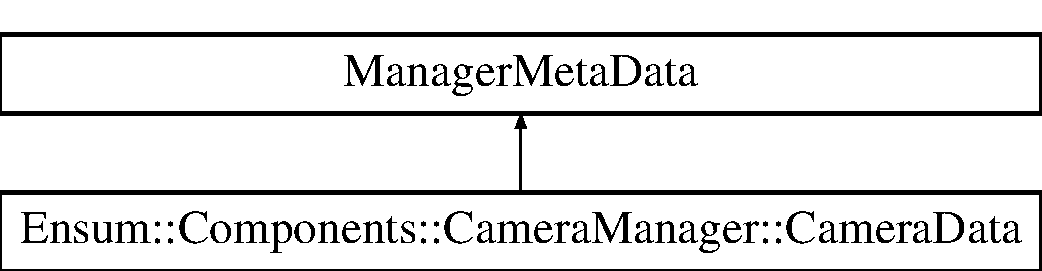
\includegraphics[height=2.000000cm]{struct_ensum_1_1_components_1_1_camera_manager_1_1_camera_data}
\end{center}
\end{figure}
\subsection*{Public Attributes}
\begin{DoxyCompactItemize}
\item 
float $\ast$ {\bfseries fov}\hypertarget{struct_ensum_1_1_components_1_1_camera_manager_1_1_camera_data_a08a315ffdf37477ee4eb888fe4fe8595}{}\label{struct_ensum_1_1_components_1_1_camera_manager_1_1_camera_data_a08a315ffdf37477ee4eb888fe4fe8595}

\item 
float $\ast$ {\bfseries aspect}\hypertarget{struct_ensum_1_1_components_1_1_camera_manager_1_1_camera_data_a8afac1fd6c81b74a571d93eecd782800}{}\label{struct_ensum_1_1_components_1_1_camera_manager_1_1_camera_data_a8afac1fd6c81b74a571d93eecd782800}

\item 
float $\ast$ {\bfseries nearp}\hypertarget{struct_ensum_1_1_components_1_1_camera_manager_1_1_camera_data_a4aaaab410e439c1668cacf65983b2946}{}\label{struct_ensum_1_1_components_1_1_camera_manager_1_1_camera_data_a4aaaab410e439c1668cacf65983b2946}

\item 
float $\ast$ {\bfseries view\+Distance}\hypertarget{struct_ensum_1_1_components_1_1_camera_manager_1_1_camera_data_a11195cfa295086337c39280d26da15d6}{}\label{struct_ensum_1_1_components_1_1_camera_manager_1_1_camera_data_a11195cfa295086337c39280d26da15d6}

\item 
bool $\ast$ {\bfseries controllable}\hypertarget{struct_ensum_1_1_components_1_1_camera_manager_1_1_camera_data_aebb098f455a07deae4bdc729c412d287}{}\label{struct_ensum_1_1_components_1_1_camera_manager_1_1_camera_data_aebb098f455a07deae4bdc729c412d287}

\item 
Direct\+X\+::\+X\+M\+F\+L\+O\+A\+T4\+X4 $\ast$ {\bfseries view\+Matrix}\hypertarget{struct_ensum_1_1_components_1_1_camera_manager_1_1_camera_data_a085caffdc6d908e9843302b5db9214ff}{}\label{struct_ensum_1_1_components_1_1_camera_manager_1_1_camera_data_a085caffdc6d908e9843302b5db9214ff}

\item 
Direct\+X\+::\+X\+M\+F\+L\+O\+A\+T4\+X4 $\ast$ {\bfseries projection\+Matrix}\hypertarget{struct_ensum_1_1_components_1_1_camera_manager_1_1_camera_data_ae92083a9c6434f43a725c3ba73d49c3a}{}\label{struct_ensum_1_1_components_1_1_camera_manager_1_1_camera_data_ae92083a9c6434f43a725c3ba73d49c3a}

\item 
Direct\+X\+::\+X\+M\+F\+L\+O\+A\+T4\+X4 $\ast$ {\bfseries view\+Projection\+Matrix}\hypertarget{struct_ensum_1_1_components_1_1_camera_manager_1_1_camera_data_a855082c74369f99dc413d34869c4fd21}{}\label{struct_ensum_1_1_components_1_1_camera_manager_1_1_camera_data_a855082c74369f99dc413d34869c4fd21}

\end{DoxyCompactItemize}


\subsection{Detailed Description}
The managers data struct. 

The documentation for this struct was generated from the following file\+:\begin{DoxyCompactItemize}
\item 
C\+:/\+Users/peter/\+Source/\+Repos/\+E\+N\+S\+U\+M/\+Ensum/\+Includes/\+Ensum\+\_\+components/Camera\+Manager.\+h\end{DoxyCompactItemize}

\hypertarget{class_ensum_1_1_components_1_1_camera_manager}{}\section{Ensum\+:\+:Components\+:\+:Camera\+Manager Class Reference}
\label{class_ensum_1_1_components_1_1_camera_manager}\index{Ensum\+::\+Components\+::\+Camera\+Manager@{Ensum\+::\+Components\+::\+Camera\+Manager}}


Camera component, holds the view, projection, etc.  




{\ttfamily \#include $<$Camera\+Manager.\+h$>$}

Inheritance diagram for Ensum\+:\+:Components\+:\+:Camera\+Manager\+:\begin{figure}[H]
\begin{center}
\leavevmode
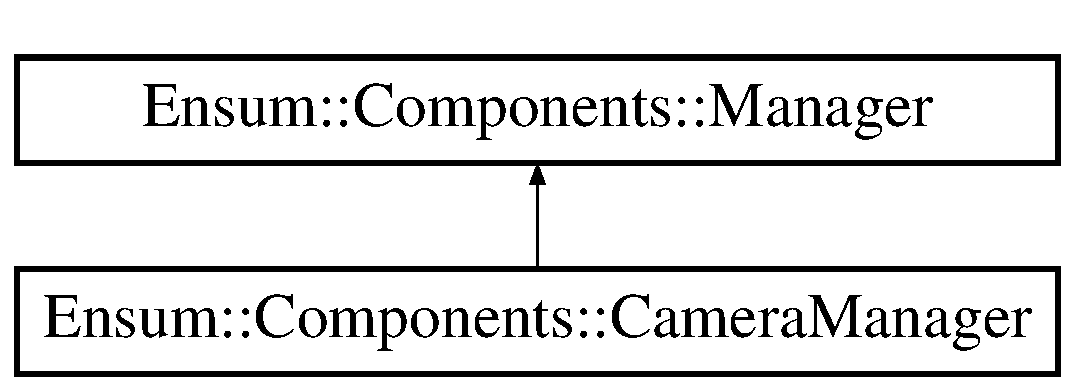
\includegraphics[height=2.000000cm]{class_ensum_1_1_components_1_1_camera_manager}
\end{center}
\end{figure}
\subsection*{Classes}
\begin{DoxyCompactItemize}
\item 
struct \hyperlink{struct_ensum_1_1_components_1_1_camera_manager_1_1_camera_data}{Camera\+Data}
\begin{DoxyCompactList}\small\item\em The managers data struct. \end{DoxyCompactList}\end{DoxyCompactItemize}
\subsection*{Public Member Functions}
\begin{DoxyCompactItemize}
\item 
{\bfseries Camera\+Manager} (\hyperlink{class_ensum_1_1_components_1_1_entity_manager}{Entity\+Manager} \&ent\+Manager, \hyperlink{class_ensum_1_1_components_1_1_transform_manager}{Transform\+Manager} \&transform\+Manager, \hyperlink{class_ensum_1_1_input_1_1_input}{Input\+::\+Input} \&input)\hypertarget{class_ensum_1_1_components_1_1_camera_manager_ac7b03cc416c4cd3eb033356c2c49d4c1}{}\label{class_ensum_1_1_components_1_1_camera_manager_ac7b03cc416c4cd3eb033356c2c49d4c1}

\item 
const void \hyperlink{class_ensum_1_1_components_1_1_camera_manager_a47e425d0c9ec790f6e54f813c601d28b}{Create\+Controllable\+Camera} (const \hyperlink{struct_ensum_1_1_components_1_1_entity}{Entity} \&entity)
\begin{DoxyCompactList}\small\item\em Create a camera which accepts player input. \end{DoxyCompactList}\item 
const void \hyperlink{class_ensum_1_1_components_1_1_camera_manager_a7e18a054f3dff83b2766df1d79093026}{Create\+Un\+Controllable\+Camera} (const \hyperlink{struct_ensum_1_1_components_1_1_entity}{Entity} \&entity)
\begin{DoxyCompactList}\small\item\em Create a camera that only get its orientation from the translation. \end{DoxyCompactList}\end{DoxyCompactItemize}
\subsection*{Private Member Functions}
\begin{DoxyCompactItemize}
\item 
const void \hyperlink{class_ensum_1_1_components_1_1_camera_manager_a1ccb090150e77084806fa903bc5006e5}{\+\_\+\+Allocate} (uint32\+\_\+t size)\hypertarget{class_ensum_1_1_components_1_1_camera_manager_a1ccb090150e77084806fa903bc5006e5}{}\label{class_ensum_1_1_components_1_1_camera_manager_a1ccb090150e77084806fa903bc5006e5}

\begin{DoxyCompactList}\small\item\em Allocate more memory. \end{DoxyCompactList}\item 
const void \hyperlink{class_ensum_1_1_components_1_1_camera_manager_a7a4aff38cf9e0fa2d504e0836d06efe7}{\+\_\+\+Destroy} (uint32\+\_\+t index)
\begin{DoxyCompactList}\small\item\em Delete an entry in the memory block. \end{DoxyCompactList}\item 
const void \hyperlink{class_ensum_1_1_components_1_1_camera_manager_af3d4e192ed57eccef18ae37bbb6377e2}{Frame} ()
\begin{DoxyCompactList}\small\item\em Takes input for player controlled camera. \end{DoxyCompactList}\item 
const void \hyperlink{class_ensum_1_1_components_1_1_camera_manager_a59015c858649a55264cb89f0338d5b96}{\+\_\+\+On\+Options\+Change} ()\hypertarget{class_ensum_1_1_components_1_1_camera_manager_a59015c858649a55264cb89f0338d5b96}{}\label{class_ensum_1_1_components_1_1_camera_manager_a59015c858649a55264cb89f0338d5b96}

\begin{DoxyCompactList}\small\item\em Called when options have changed. \end{DoxyCompactList}\end{DoxyCompactItemize}
\subsection*{Private Attributes}
\begin{DoxyCompactItemize}
\item 
\hyperlink{struct_ensum_1_1_components_1_1_camera_manager_1_1_camera_data}{Camera\+Data} $\ast$ \hyperlink{class_ensum_1_1_components_1_1_camera_manager_a370c6e1c497262287af591821ac42d09}{\+\_\+datap}
\item 
\hyperlink{class_ensum_1_1_components_1_1_transform_manager}{Transform\+Manager} \& {\bfseries \+\_\+transform\+Manager}\hypertarget{class_ensum_1_1_components_1_1_camera_manager_a2664fa2e0c57e893408fd1d98b594055}{}\label{class_ensum_1_1_components_1_1_camera_manager_a2664fa2e0c57e893408fd1d98b594055}

\item 
\hyperlink{class_ensum_1_1_input_1_1_input}{Input\+::\+Input} \& {\bfseries \+\_\+input}\hypertarget{class_ensum_1_1_components_1_1_camera_manager_a43ae22b81db7c864e876b1f108f7d5bf}{}\label{class_ensum_1_1_components_1_1_camera_manager_a43ae22b81db7c864e876b1f108f7d5bf}

\end{DoxyCompactItemize}
\subsection*{Additional Inherited Members}


\subsection{Detailed Description}
Camera component, holds the view, projection, etc. 

For rendering. 

\subsection{Member Function Documentation}
\index{Ensum\+::\+Components\+::\+Camera\+Manager@{Ensum\+::\+Components\+::\+Camera\+Manager}!\+\_\+\+Destroy@{\+\_\+\+Destroy}}
\index{\+\_\+\+Destroy@{\+\_\+\+Destroy}!Ensum\+::\+Components\+::\+Camera\+Manager@{Ensum\+::\+Components\+::\+Camera\+Manager}}
\subsubsection[{\texorpdfstring{\+\_\+\+Destroy(uint32\+\_\+t index)}{_Destroy(uint32_t index)}}]{\setlength{\rightskip}{0pt plus 5cm}const void Ensum\+::\+Components\+::\+Camera\+Manager\+::\+\_\+\+Destroy (
\begin{DoxyParamCaption}
\item[{uint32\+\_\+t}]{index}
\end{DoxyParamCaption}
)\hspace{0.3cm}{\ttfamily [private]}, {\ttfamily [virtual]}}\hypertarget{class_ensum_1_1_components_1_1_camera_manager_a7a4aff38cf9e0fa2d504e0836d06efe7}{}\label{class_ensum_1_1_components_1_1_camera_manager_a7a4aff38cf9e0fa2d504e0836d06efe7}


Delete an entry in the memory block. 

The deleted entry is replaced by the last in the block. 

Implements \hyperlink{class_ensum_1_1_components_1_1_manager_a5ba85395802e942ed8904ca18951e6b0}{Ensum\+::\+Components\+::\+Manager}.

\index{Ensum\+::\+Components\+::\+Camera\+Manager@{Ensum\+::\+Components\+::\+Camera\+Manager}!Create\+Controllable\+Camera@{Create\+Controllable\+Camera}}
\index{Create\+Controllable\+Camera@{Create\+Controllable\+Camera}!Ensum\+::\+Components\+::\+Camera\+Manager@{Ensum\+::\+Components\+::\+Camera\+Manager}}
\subsubsection[{\texorpdfstring{Create\+Controllable\+Camera(const Entity \&entity)}{CreateControllableCamera(const Entity &entity)}}]{\setlength{\rightskip}{0pt plus 5cm}const void Ensum\+::\+Components\+::\+Camera\+Manager\+::\+Create\+Controllable\+Camera (
\begin{DoxyParamCaption}
\item[{const {\bf Entity} \&}]{entity}
\end{DoxyParamCaption}
)}\hypertarget{class_ensum_1_1_components_1_1_camera_manager_a47e425d0c9ec790f6e54f813c601d28b}{}\label{class_ensum_1_1_components_1_1_camera_manager_a47e425d0c9ec790f6e54f813c601d28b}


Create a camera which accepts player input. 

(Player camera,etc.) \index{Ensum\+::\+Components\+::\+Camera\+Manager@{Ensum\+::\+Components\+::\+Camera\+Manager}!Create\+Un\+Controllable\+Camera@{Create\+Un\+Controllable\+Camera}}
\index{Create\+Un\+Controllable\+Camera@{Create\+Un\+Controllable\+Camera}!Ensum\+::\+Components\+::\+Camera\+Manager@{Ensum\+::\+Components\+::\+Camera\+Manager}}
\subsubsection[{\texorpdfstring{Create\+Un\+Controllable\+Camera(const Entity \&entity)}{CreateUnControllableCamera(const Entity &entity)}}]{\setlength{\rightskip}{0pt plus 5cm}const void Ensum\+::\+Components\+::\+Camera\+Manager\+::\+Create\+Un\+Controllable\+Camera (
\begin{DoxyParamCaption}
\item[{const {\bf Entity} \&}]{entity}
\end{DoxyParamCaption}
)}\hypertarget{class_ensum_1_1_components_1_1_camera_manager_a7e18a054f3dff83b2766df1d79093026}{}\label{class_ensum_1_1_components_1_1_camera_manager_a7e18a054f3dff83b2766df1d79093026}


Create a camera that only get its orientation from the translation. 

(Security camera,etc.) \index{Ensum\+::\+Components\+::\+Camera\+Manager@{Ensum\+::\+Components\+::\+Camera\+Manager}!Frame@{Frame}}
\index{Frame@{Frame}!Ensum\+::\+Components\+::\+Camera\+Manager@{Ensum\+::\+Components\+::\+Camera\+Manager}}
\subsubsection[{\texorpdfstring{Frame()}{Frame()}}]{\setlength{\rightskip}{0pt plus 5cm}const void Ensum\+::\+Components\+::\+Camera\+Manager\+::\+Frame (
\begin{DoxyParamCaption}
{}
\end{DoxyParamCaption}
)\hspace{0.3cm}{\ttfamily [private]}, {\ttfamily [virtual]}}\hypertarget{class_ensum_1_1_components_1_1_camera_manager_af3d4e192ed57eccef18ae37bbb6377e2}{}\label{class_ensum_1_1_components_1_1_camera_manager_af3d4e192ed57eccef18ae37bbb6377e2}


Takes input for player controlled camera. 

Also calls the garbadge collection func. 

Reimplemented from \hyperlink{class_ensum_1_1_components_1_1_manager_a7327f9a28abf0011498ced0c86692a73}{Ensum\+::\+Components\+::\+Manager}.



\subsection{Member Data Documentation}
\index{Ensum\+::\+Components\+::\+Camera\+Manager@{Ensum\+::\+Components\+::\+Camera\+Manager}!\+\_\+datap@{\+\_\+datap}}
\index{\+\_\+datap@{\+\_\+datap}!Ensum\+::\+Components\+::\+Camera\+Manager@{Ensum\+::\+Components\+::\+Camera\+Manager}}
\subsubsection[{\texorpdfstring{\+\_\+datap}{_datap}}]{\setlength{\rightskip}{0pt plus 5cm}{\bf Camera\+Data}$\ast$ Ensum\+::\+Components\+::\+Camera\+Manager\+::\+\_\+datap\hspace{0.3cm}{\ttfamily [private]}}\hypertarget{class_ensum_1_1_components_1_1_camera_manager_a370c6e1c497262287af591821ac42d09}{}\label{class_ensum_1_1_components_1_1_camera_manager_a370c6e1c497262287af591821ac42d09}
A reference pointer to avoid having to cast the basic datapointer all the time. 

The documentation for this class was generated from the following file\+:\begin{DoxyCompactItemize}
\item 
C\+:/\+Users/peter/\+Source/\+Repos/\+E\+N\+S\+U\+M/\+Ensum/\+Includes/\+Ensum\+\_\+components/Camera\+Manager.\+h\end{DoxyCompactItemize}

\hypertarget{struct_ensum_1_1_graphics_1_1_direct3_d12_1_1_c_d3_d12___c_p_u___d_e_s_c_r_i_p_t_o_r___h_a_n_d_l_e}{}\section{Ensum\+:\+:Graphics\+:\+:Direct3\+D12\+:\+:C\+D3\+D12\+\_\+\+C\+P\+U\+\_\+\+D\+E\+S\+C\+R\+I\+P\+T\+O\+R\+\_\+\+H\+A\+N\+D\+LE Struct Reference}
\label{struct_ensum_1_1_graphics_1_1_direct3_d12_1_1_c_d3_d12___c_p_u___d_e_s_c_r_i_p_t_o_r___h_a_n_d_l_e}\index{Ensum\+::\+Graphics\+::\+Direct3\+D12\+::\+C\+D3\+D12\+\_\+\+C\+P\+U\+\_\+\+D\+E\+S\+C\+R\+I\+P\+T\+O\+R\+\_\+\+H\+A\+N\+D\+LE@{Ensum\+::\+Graphics\+::\+Direct3\+D12\+::\+C\+D3\+D12\+\_\+\+C\+P\+U\+\_\+\+D\+E\+S\+C\+R\+I\+P\+T\+O\+R\+\_\+\+H\+A\+N\+D\+LE}}
\subsection*{Public Member Functions}
\begin{DoxyCompactItemize}
\item 
{\bfseries C\+D3\+D12\+\_\+\+C\+P\+U\+\_\+\+D\+E\+S\+C\+R\+I\+P\+T\+O\+R\+\_\+\+H\+A\+N\+D\+LE} (D3\+D12\+\_\+\+C\+P\+U\+\_\+\+D\+E\+S\+C\+R\+I\+P\+T\+O\+R\+\_\+\+H\+A\+N\+D\+LE h)\hypertarget{struct_ensum_1_1_graphics_1_1_direct3_d12_1_1_c_d3_d12___c_p_u___d_e_s_c_r_i_p_t_o_r___h_a_n_d_l_e_a01bd224f75bf7842350de95121f4dfcf}{}\label{struct_ensum_1_1_graphics_1_1_direct3_d12_1_1_c_d3_d12___c_p_u___d_e_s_c_r_i_p_t_o_r___h_a_n_d_l_e_a01bd224f75bf7842350de95121f4dfcf}

\item 
{\bfseries C\+D3\+D12\+\_\+\+C\+P\+U\+\_\+\+D\+E\+S\+C\+R\+I\+P\+T\+O\+R\+\_\+\+H\+A\+N\+D\+LE} (D3\+D12\+\_\+\+C\+P\+U\+\_\+\+D\+E\+S\+C\+R\+I\+P\+T\+O\+R\+\_\+\+H\+A\+N\+D\+LE h, size\+\_\+t curr, size\+\_\+t size)\hypertarget{struct_ensum_1_1_graphics_1_1_direct3_d12_1_1_c_d3_d12___c_p_u___d_e_s_c_r_i_p_t_o_r___h_a_n_d_l_e_ab90bca624384c3162583a000044d2dce}{}\label{struct_ensum_1_1_graphics_1_1_direct3_d12_1_1_c_d3_d12___c_p_u___d_e_s_c_r_i_p_t_o_r___h_a_n_d_l_e_ab90bca624384c3162583a000044d2dce}

\item 
const void {\bfseries Offset} (size\+\_\+t curr, size\+\_\+t size)\hypertarget{struct_ensum_1_1_graphics_1_1_direct3_d12_1_1_c_d3_d12___c_p_u___d_e_s_c_r_i_p_t_o_r___h_a_n_d_l_e_a8ca593a4b65c813941433d3a7f36f940}{}\label{struct_ensum_1_1_graphics_1_1_direct3_d12_1_1_c_d3_d12___c_p_u___d_e_s_c_r_i_p_t_o_r___h_a_n_d_l_e_a8ca593a4b65c813941433d3a7f36f940}

\item 
{\bfseries operator D3\+D12\+\_\+\+C\+P\+U\+\_\+\+D\+E\+S\+C\+R\+I\+P\+T\+O\+R\+\_\+\+H\+A\+N\+D\+LE} ()\hypertarget{struct_ensum_1_1_graphics_1_1_direct3_d12_1_1_c_d3_d12___c_p_u___d_e_s_c_r_i_p_t_o_r___h_a_n_d_l_e_a2672d9462146a5ad1b923131a794354b}{}\label{struct_ensum_1_1_graphics_1_1_direct3_d12_1_1_c_d3_d12___c_p_u___d_e_s_c_r_i_p_t_o_r___h_a_n_d_l_e_a2672d9462146a5ad1b923131a794354b}

\end{DoxyCompactItemize}
\subsection*{Public Attributes}
\begin{DoxyCompactItemize}
\item 
D3\+D12\+\_\+\+C\+P\+U\+\_\+\+D\+E\+S\+C\+R\+I\+P\+T\+O\+R\+\_\+\+H\+A\+N\+D\+LE {\bfseries handle}\hypertarget{struct_ensum_1_1_graphics_1_1_direct3_d12_1_1_c_d3_d12___c_p_u___d_e_s_c_r_i_p_t_o_r___h_a_n_d_l_e_a74a4a3247d83196478b6d7615d1aa036}{}\label{struct_ensum_1_1_graphics_1_1_direct3_d12_1_1_c_d3_d12___c_p_u___d_e_s_c_r_i_p_t_o_r___h_a_n_d_l_e_a74a4a3247d83196478b6d7615d1aa036}

\end{DoxyCompactItemize}


The documentation for this struct was generated from the following file\+:\begin{DoxyCompactItemize}
\item 
C\+:/\+Users/peter/\+Source/\+Repos/\+E\+N\+S\+U\+M/\+Ensum/\+Includes/\+Ensum\+\_\+graphics/Direct3\+D12.\+h\end{DoxyCompactItemize}

\hypertarget{class_ensum_1_1_utils_1_1_console_log}{}\section{Ensum\+:\+:Utils\+:\+:Console\+Log Class Reference}
\label{class_ensum_1_1_utils_1_1_console_log}\index{Ensum\+::\+Utils\+::\+Console\+Log@{Ensum\+::\+Utils\+::\+Console\+Log}}


Debug console.  




{\ttfamily \#include $<$Console\+Log.\+h$>$}

\subsection*{Public Member Functions}
\begin{DoxyCompactItemize}
\item 
const void \hyperlink{class_ensum_1_1_utils_1_1_console_log_af018fe2d5f702995ce18d4e2f2dde55c}{Add\+To\+Que} (const \hyperlink{class_ensum_1_1string}{string} \&data)\hypertarget{class_ensum_1_1_utils_1_1_console_log_af018fe2d5f702995ce18d4e2f2dde55c}{}\label{class_ensum_1_1_utils_1_1_console_log_af018fe2d5f702995ce18d4e2f2dde55c}

\begin{DoxyCompactList}\small\item\em Adds the string data to the que. \end{DoxyCompactList}\item 
const void \hyperlink{class_ensum_1_1_utils_1_1_console_log_a6d0cb31da153393c122cd5f9514eb6c9}{Write} ()
\begin{DoxyCompactList}\small\item\em Writes the first items in the que to the console, then deletes it. \end{DoxyCompactList}\end{DoxyCompactItemize}
\subsection*{Static Public Member Functions}
\begin{DoxyCompactItemize}
\item 
static const void \hyperlink{class_ensum_1_1_utils_1_1_console_log_a2081398f0762150043b92047fa97810a}{Create\+Instance} ()\hypertarget{class_ensum_1_1_utils_1_1_console_log_a2081398f0762150043b92047fa97810a}{}\label{class_ensum_1_1_utils_1_1_console_log_a2081398f0762150043b92047fa97810a}

\begin{DoxyCompactList}\small\item\em Creates the console. \end{DoxyCompactList}\item 
static const void \hyperlink{class_ensum_1_1_utils_1_1_console_log_a5510d37e7c7038a022e9ff23f097263d}{Delete\+Instance} ()\hypertarget{class_ensum_1_1_utils_1_1_console_log_a5510d37e7c7038a022e9ff23f097263d}{}\label{class_ensum_1_1_utils_1_1_console_log_a5510d37e7c7038a022e9ff23f097263d}

\begin{DoxyCompactList}\small\item\em Deletes the console. \end{DoxyCompactList}\item 
static const void \hyperlink{class_ensum_1_1_utils_1_1_console_log_a3cb3fc27bd5a6a1a04831e6eb8d79b42}{Dump\+To\+Console} (const char $\ast$message,...)
\begin{DoxyCompactList}\small\item\em Adds the message and optional args to the que. \end{DoxyCompactList}\item 
static const void \hyperlink{class_ensum_1_1_utils_1_1_console_log_ae4cb4119e99b9cdfd71878b5c666523f}{Dump\+To\+Console} (const W\+C\+H\+AR $\ast$message,...)
\begin{DoxyCompactList}\small\item\em Adds the message and optional args to the que. \end{DoxyCompactList}\end{DoxyCompactItemize}
\subsection*{Private Attributes}
\begin{DoxyCompactItemize}
\item 
std\+::deque$<$ \hyperlink{class_ensum_1_1string}{string} $>$ $\ast$ {\bfseries \+\_\+to\+Print}\hypertarget{class_ensum_1_1_utils_1_1_console_log_a8be721f764eb1f8330d4a2646a840a5d}{}\label{class_ensum_1_1_utils_1_1_console_log_a8be721f764eb1f8330d4a2646a840a5d}

\item 
H\+A\+N\+D\+LE {\bfseries \+\_\+thread\+Handle}\hypertarget{class_ensum_1_1_utils_1_1_console_log_aa93afd55081441f111fc804da614913e}{}\label{class_ensum_1_1_utils_1_1_console_log_aa93afd55081441f111fc804da614913e}

\item 
H\+A\+N\+D\+LE {\bfseries \+\_\+write\+Mutex}\hypertarget{class_ensum_1_1_utils_1_1_console_log_a1b8a903c69d744529d98d29f728cafcf}{}\label{class_ensum_1_1_utils_1_1_console_log_a1b8a903c69d744529d98d29f728cafcf}

\item 
D\+W\+O\+RD {\bfseries \+\_\+thread\+Address}\hypertarget{class_ensum_1_1_utils_1_1_console_log_a5258e193fd534462a6f5ff3a3a0a9072}{}\label{class_ensum_1_1_utils_1_1_console_log_a5258e193fd534462a6f5ff3a3a0a9072}

\item 
bool {\bfseries \+\_\+shutdown}\hypertarget{class_ensum_1_1_utils_1_1_console_log_abfe63ce28323a8554b5515ef684e582e}{}\label{class_ensum_1_1_utils_1_1_console_log_abfe63ce28323a8554b5515ef684e582e}

\end{DoxyCompactItemize}
\subsection*{Static Private Attributes}
\begin{DoxyCompactItemize}
\item 
static \hyperlink{class_ensum_1_1_utils_1_1_console_log}{Console\+Log} $\ast$ {\bfseries \+\_\+instance}\hypertarget{class_ensum_1_1_utils_1_1_console_log_ace276a80cd230798d08539f05816cdcb}{}\label{class_ensum_1_1_utils_1_1_console_log_ace276a80cd230798d08539f05816cdcb}

\end{DoxyCompactItemize}


\subsection{Detailed Description}
Debug console. 

\subsection{Member Function Documentation}
\index{Ensum\+::\+Utils\+::\+Console\+Log@{Ensum\+::\+Utils\+::\+Console\+Log}!Dump\+To\+Console@{Dump\+To\+Console}}
\index{Dump\+To\+Console@{Dump\+To\+Console}!Ensum\+::\+Utils\+::\+Console\+Log@{Ensum\+::\+Utils\+::\+Console\+Log}}
\subsubsection[{\texorpdfstring{Dump\+To\+Console(const char $\ast$message,...)}{DumpToConsole(const char *message,...)}}]{\setlength{\rightskip}{0pt plus 5cm}static const void Ensum\+::\+Utils\+::\+Console\+Log\+::\+Dump\+To\+Console (
\begin{DoxyParamCaption}
\item[{const char $\ast$}]{message, }
\item[{}]{...}
\end{DoxyParamCaption}
)\hspace{0.3cm}{\ttfamily [static]}}\hypertarget{class_ensum_1_1_utils_1_1_console_log_a3cb3fc27bd5a6a1a04831e6eb8d79b42}{}\label{class_ensum_1_1_utils_1_1_console_log_a3cb3fc27bd5a6a1a04831e6eb8d79b42}


Adds the message and optional args to the que. 

Use this static function when writing to the console. This is a formated string. (See documentation for printf). \index{Ensum\+::\+Utils\+::\+Console\+Log@{Ensum\+::\+Utils\+::\+Console\+Log}!Dump\+To\+Console@{Dump\+To\+Console}}
\index{Dump\+To\+Console@{Dump\+To\+Console}!Ensum\+::\+Utils\+::\+Console\+Log@{Ensum\+::\+Utils\+::\+Console\+Log}}
\subsubsection[{\texorpdfstring{Dump\+To\+Console(const W\+C\+H\+A\+R $\ast$message,...)}{DumpToConsole(const WCHAR *message,...)}}]{\setlength{\rightskip}{0pt plus 5cm}static const void Ensum\+::\+Utils\+::\+Console\+Log\+::\+Dump\+To\+Console (
\begin{DoxyParamCaption}
\item[{const W\+C\+H\+AR $\ast$}]{message, }
\item[{}]{...}
\end{DoxyParamCaption}
)\hspace{0.3cm}{\ttfamily [static]}}\hypertarget{class_ensum_1_1_utils_1_1_console_log_ae4cb4119e99b9cdfd71878b5c666523f}{}\label{class_ensum_1_1_utils_1_1_console_log_ae4cb4119e99b9cdfd71878b5c666523f}


Adds the message and optional args to the que. 

Use this static function when writing to the console. This is a formated string. (See documentation for printf). \index{Ensum\+::\+Utils\+::\+Console\+Log@{Ensum\+::\+Utils\+::\+Console\+Log}!Write@{Write}}
\index{Write@{Write}!Ensum\+::\+Utils\+::\+Console\+Log@{Ensum\+::\+Utils\+::\+Console\+Log}}
\subsubsection[{\texorpdfstring{Write()}{Write()}}]{\setlength{\rightskip}{0pt plus 5cm}const void Ensum\+::\+Utils\+::\+Console\+Log\+::\+Write (
\begin{DoxyParamCaption}
{}
\end{DoxyParamCaption}
)}\hypertarget{class_ensum_1_1_utils_1_1_console_log_a6d0cb31da153393c122cd5f9514eb6c9}{}\label{class_ensum_1_1_utils_1_1_console_log_a6d0cb31da153393c122cd5f9514eb6c9}


Writes the first items in the que to the console, then deletes it. 

This is used in the thread. 

The documentation for this class was generated from the following file\+:\begin{DoxyCompactItemize}
\item 
C\+:/\+Users/peter/\+Source/\+Repos/\+E\+N\+S\+U\+M/\+Ensum/\+Includes/\+Ensum\+\_\+utils/Console\+Log.\+h\end{DoxyCompactItemize}

\hypertarget{class_ensum_1_1_graphics_1_1_d3_d11}{}\section{Ensum\+:\+:Graphics\+:\+:D3\+D11 Class Reference}
\label{class_ensum_1_1_graphics_1_1_d3_d11}\index{Ensum\+::\+Graphics\+::\+D3\+D11@{Ensum\+::\+Graphics\+::\+D3\+D11}}
Inheritance diagram for Ensum\+:\+:Graphics\+:\+:D3\+D11\+:\begin{figure}[H]
\begin{center}
\leavevmode
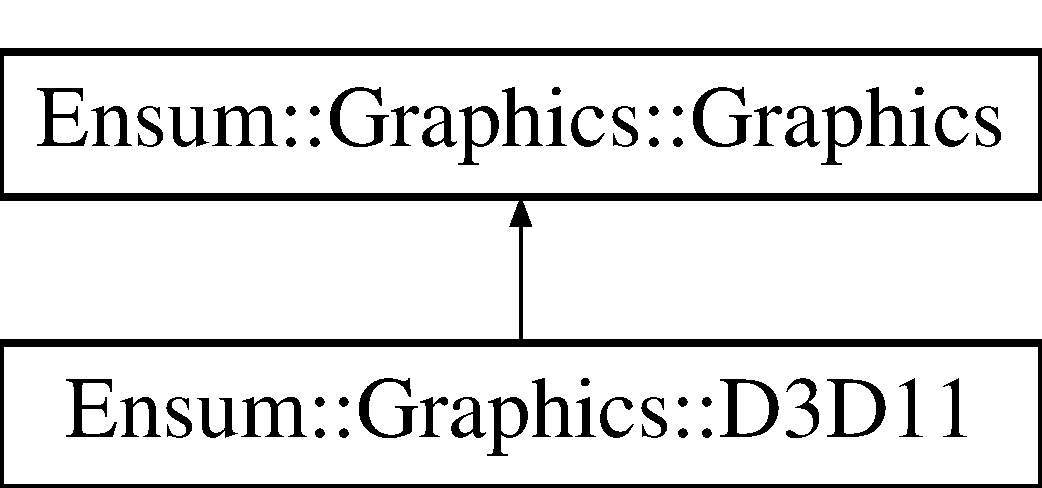
\includegraphics[height=2.000000cm]{class_ensum_1_1_graphics_1_1_d3_d11}
\end{center}
\end{figure}
\subsection*{Public Member Functions}
\begin{DoxyCompactItemize}
\item 
virtual const void \hyperlink{class_ensum_1_1_graphics_1_1_d3_d11_acd6cd3569d5c0dfc50398b3828578990}{On\+Create\+Device} ()\hypertarget{class_ensum_1_1_graphics_1_1_d3_d11_acd6cd3569d5c0dfc50398b3828578990}{}\label{class_ensum_1_1_graphics_1_1_d3_d11_acd6cd3569d5c0dfc50398b3828578990}

\begin{DoxyCompactList}\small\item\em Create all the graphics stuff. \end{DoxyCompactList}\item 
virtual const void \hyperlink{class_ensum_1_1_graphics_1_1_d3_d11_a302b7c773ae06b4344324d4a94ea7aa1}{On\+Destroy\+Device} ()\hypertarget{class_ensum_1_1_graphics_1_1_d3_d11_a302b7c773ae06b4344324d4a94ea7aa1}{}\label{class_ensum_1_1_graphics_1_1_d3_d11_a302b7c773ae06b4344324d4a94ea7aa1}

\begin{DoxyCompactList}\small\item\em Destroy all the graphics stuff. \end{DoxyCompactList}\end{DoxyCompactItemize}
\subsection*{Protected Member Functions}
\begin{DoxyCompactItemize}
\item 
virtual const void \hyperlink{class_ensum_1_1_graphics_1_1_d3_d11_aaa1f9118226ed14729d1d1ad450ec10d}{\+\_\+\+On\+Options\+Change} ()\hypertarget{class_ensum_1_1_graphics_1_1_d3_d11_aaa1f9118226ed14729d1d1ad450ec10d}{}\label{class_ensum_1_1_graphics_1_1_d3_d11_aaa1f9118226ed14729d1d1ad450ec10d}

\begin{DoxyCompactList}\small\item\em Options change func. \end{DoxyCompactList}\item 
virtual const void \hyperlink{class_ensum_1_1_graphics_1_1_d3_d11_afea086dc974d70437a9c415473233c38}{\+\_\+\+Begin\+Frame} (void)\hypertarget{class_ensum_1_1_graphics_1_1_d3_d11_afea086dc974d70437a9c415473233c38}{}\label{class_ensum_1_1_graphics_1_1_d3_d11_afea086dc974d70437a9c415473233c38}

\begin{DoxyCompactList}\small\item\em Begin the frame. \end{DoxyCompactList}\item 
virtual const void \hyperlink{class_ensum_1_1_graphics_1_1_d3_d11_a5a64baccb2481676a72de24548f03728}{\+\_\+\+End\+Frame} (void)\hypertarget{class_ensum_1_1_graphics_1_1_d3_d11_a5a64baccb2481676a72de24548f03728}{}\label{class_ensum_1_1_graphics_1_1_d3_d11_a5a64baccb2481676a72de24548f03728}

\begin{DoxyCompactList}\small\item\em End the frame. \end{DoxyCompactList}\item 
virtual const void \hyperlink{class_ensum_1_1_graphics_1_1_d3_d11_a234588ad9a96acd36260f766e5b7f839}{\+\_\+\+Frame} ()\hypertarget{class_ensum_1_1_graphics_1_1_d3_d11_a234588ad9a96acd36260f766e5b7f839}{}\label{class_ensum_1_1_graphics_1_1_d3_d11_a234588ad9a96acd36260f766e5b7f839}

\begin{DoxyCompactList}\small\item\em Render everything. \end{DoxyCompactList}\end{DoxyCompactItemize}
\subsection*{Protected Attributes}
\begin{DoxyCompactItemize}
\item 
\hyperlink{class_ensum_1_1_graphics_1_1_direct3_d11}{Direct3\+D11} {\bfseries \+\_\+\+D3\+D11}\hypertarget{class_ensum_1_1_graphics_1_1_d3_d11_a4b546673d48ed239e6704743e901be3e}{}\label{class_ensum_1_1_graphics_1_1_d3_d11_a4b546673d48ed239e6704743e901be3e}

\end{DoxyCompactItemize}
\subsection*{Additional Inherited Members}


The documentation for this class was generated from the following file\+:\begin{DoxyCompactItemize}
\item 
C\+:/\+Users/peter/\+Source/\+Repos/\+E\+N\+S\+U\+M/\+Ensum/\+Includes/\+Ensum\+\_\+graphics/D3\+D11.\+h\end{DoxyCompactItemize}

\hypertarget{class_ensum_1_1_graphics_1_1_d3_d12}{}\section{Ensum\+:\+:Graphics\+:\+:D3\+D12 Class Reference}
\label{class_ensum_1_1_graphics_1_1_d3_d12}\index{Ensum\+::\+Graphics\+::\+D3\+D12@{Ensum\+::\+Graphics\+::\+D3\+D12}}
Inheritance diagram for Ensum\+:\+:Graphics\+:\+:D3\+D12\+:\begin{figure}[H]
\begin{center}
\leavevmode
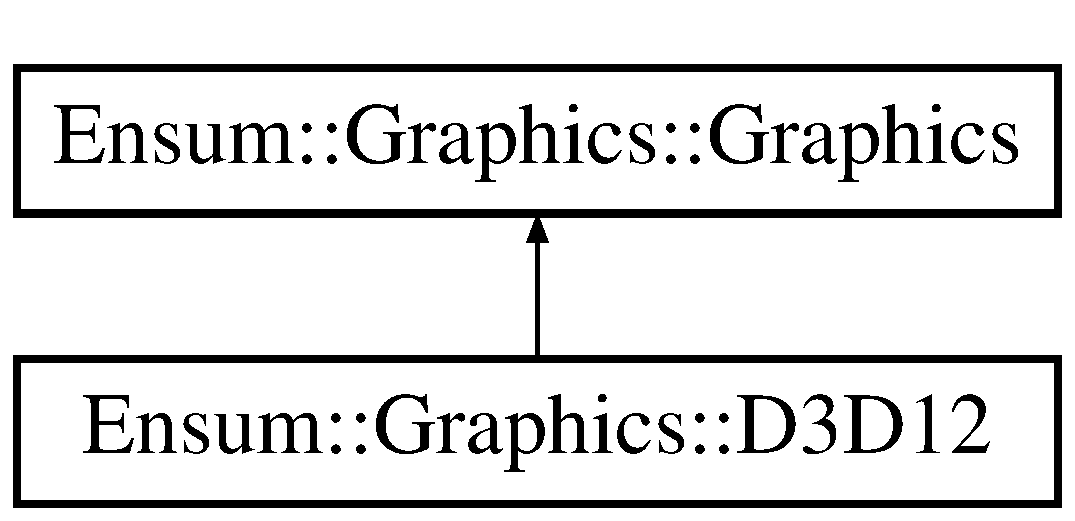
\includegraphics[height=2.000000cm]{class_ensum_1_1_graphics_1_1_d3_d12}
\end{center}
\end{figure}
\subsection*{Classes}
\begin{DoxyCompactItemize}
\item 
struct \hyperlink{struct_ensum_1_1_graphics_1_1_d3_d12_1_1_buffer_data}{Buffer\+Data}
\item 
struct \hyperlink{struct_ensum_1_1_graphics_1_1_d3_d12_1_1_vertex}{Vertex}
\end{DoxyCompactItemize}
\subsection*{Public Member Functions}
\begin{DoxyCompactItemize}
\item 
virtual const void \hyperlink{class_ensum_1_1_graphics_1_1_d3_d12_a566fc5ea52ee31cb32eebf8e65364460}{On\+Create\+Device} ()\hypertarget{class_ensum_1_1_graphics_1_1_d3_d12_a566fc5ea52ee31cb32eebf8e65364460}{}\label{class_ensum_1_1_graphics_1_1_d3_d12_a566fc5ea52ee31cb32eebf8e65364460}

\begin{DoxyCompactList}\small\item\em Create all the graphics stuff. \end{DoxyCompactList}\item 
virtual const void \hyperlink{class_ensum_1_1_graphics_1_1_d3_d12_a240e7a2dce61323726a41b557ee26a59}{On\+Destroy\+Device} ()\hypertarget{class_ensum_1_1_graphics_1_1_d3_d12_a240e7a2dce61323726a41b557ee26a59}{}\label{class_ensum_1_1_graphics_1_1_d3_d12_a240e7a2dce61323726a41b557ee26a59}

\begin{DoxyCompactList}\small\item\em Destroy all the graphics stuff. \end{DoxyCompactList}\end{DoxyCompactItemize}
\subsection*{Protected Member Functions}
\begin{DoxyCompactItemize}
\item 
virtual const void \hyperlink{class_ensum_1_1_graphics_1_1_d3_d12_ad276cdc2f03df54cbbb7d05ac8785df4}{\+\_\+\+On\+Options\+Change} ()
\begin{DoxyCompactList}\small\item\em Loads a mesh and creates a vertex and indexbuffer ID of mesh is returned. \end{DoxyCompactList}\item 
virtual const void \hyperlink{class_ensum_1_1_graphics_1_1_d3_d12_ae258edd552c4bf071a59a140e8f62298}{\+\_\+\+Begin\+Frame} (void)\hypertarget{class_ensum_1_1_graphics_1_1_d3_d12_ae258edd552c4bf071a59a140e8f62298}{}\label{class_ensum_1_1_graphics_1_1_d3_d12_ae258edd552c4bf071a59a140e8f62298}

\begin{DoxyCompactList}\small\item\em Begin the frame. \end{DoxyCompactList}\item 
virtual const void \hyperlink{class_ensum_1_1_graphics_1_1_d3_d12_a102d8e89d1424e4ecefd5750843fa4db}{\+\_\+\+End\+Frame} (void)\hypertarget{class_ensum_1_1_graphics_1_1_d3_d12_a102d8e89d1424e4ecefd5750843fa4db}{}\label{class_ensum_1_1_graphics_1_1_d3_d12_a102d8e89d1424e4ecefd5750843fa4db}

\begin{DoxyCompactList}\small\item\em End the frame. \end{DoxyCompactList}\item 
virtual const void \hyperlink{class_ensum_1_1_graphics_1_1_d3_d12_adcd65422dfc151bd913168c876c11f29}{\+\_\+\+Frame} ()\hypertarget{class_ensum_1_1_graphics_1_1_d3_d12_adcd65422dfc151bd913168c876c11f29}{}\label{class_ensum_1_1_graphics_1_1_d3_d12_adcd65422dfc151bd913168c876c11f29}

\begin{DoxyCompactList}\small\item\em Render everything. \end{DoxyCompactList}\end{DoxyCompactItemize}
\subsection*{Protected Attributes}
\begin{DoxyCompactItemize}
\item 
\hyperlink{class_ensum_1_1_graphics_1_1_direct3_d12}{Direct3\+D12} {\bfseries \+\_\+\+D3\+D12}\hypertarget{class_ensum_1_1_graphics_1_1_d3_d12_ad50a4d9dc6db3ce447fb6740ccfb3cf1}{}\label{class_ensum_1_1_graphics_1_1_d3_d12_ad50a4d9dc6db3ce447fb6740ccfb3cf1}

\item 
D3\+D12\+\_\+\+V\+I\+E\+W\+P\+O\+RT {\bfseries \+\_\+view\+Port}\hypertarget{class_ensum_1_1_graphics_1_1_d3_d12_a02b9cf7e0456b1fafbe39ba21f2babbd}{}\label{class_ensum_1_1_graphics_1_1_d3_d12_a02b9cf7e0456b1fafbe39ba21f2babbd}

\end{DoxyCompactItemize}
\subsection*{Additional Inherited Members}


\subsection{Member Function Documentation}
\index{Ensum\+::\+Graphics\+::\+D3\+D12@{Ensum\+::\+Graphics\+::\+D3\+D12}!\+\_\+\+On\+Options\+Change@{\+\_\+\+On\+Options\+Change}}
\index{\+\_\+\+On\+Options\+Change@{\+\_\+\+On\+Options\+Change}!Ensum\+::\+Graphics\+::\+D3\+D12@{Ensum\+::\+Graphics\+::\+D3\+D12}}
\subsubsection[{\texorpdfstring{\+\_\+\+On\+Options\+Change()}{_OnOptionsChange()}}]{\setlength{\rightskip}{0pt plus 5cm}virtual const void Ensum\+::\+Graphics\+::\+D3\+D12\+::\+\_\+\+On\+Options\+Change (
\begin{DoxyParamCaption}
{}
\end{DoxyParamCaption}
)\hspace{0.3cm}{\ttfamily [protected]}, {\ttfamily [virtual]}}\hypertarget{class_ensum_1_1_graphics_1_1_d3_d12_ad276cdc2f03df54cbbb7d05ac8785df4}{}\label{class_ensum_1_1_graphics_1_1_d3_d12_ad276cdc2f03df54cbbb7d05ac8785df4}


Loads a mesh and creates a vertex and indexbuffer ID of mesh is returned. 

Use flag to indicate loading and unloading for mesh.\+Interleave the vertex data\+Options change func. 

Implements \hyperlink{class_ensum_1_1_graphics_1_1_graphics_a530a469dbfc96e4224c916f2253b8764}{Ensum\+::\+Graphics\+::\+Graphics}.



The documentation for this class was generated from the following file\+:\begin{DoxyCompactItemize}
\item 
C\+:/\+Users/peter/\+Source/\+Repos/\+E\+N\+S\+U\+M/\+Ensum/\+Includes/\+Ensum\+\_\+graphics/D3\+D12.\+h\end{DoxyCompactItemize}

\hypertarget{struct_ensum_1_1_file_handler_1_1_data}{}\section{Ensum\+:\+:File\+Handler\+:\+:Data Struct Reference}
\label{struct_ensum_1_1_file_handler_1_1_data}\index{Ensum\+::\+File\+Handler\+::\+Data@{Ensum\+::\+File\+Handler\+::\+Data}}
\subsection*{Public Attributes}
\begin{DoxyCompactItemize}
\item 
void $\ast$ {\bfseries buffer} = nullptr\hypertarget{struct_ensum_1_1_file_handler_1_1_data_a9452d399909851b8319ee43803c74657}{}\label{struct_ensum_1_1_file_handler_1_1_data_a9452d399909851b8319ee43803c74657}

\item 
size\+\_\+t {\bfseries allocated} = 0\hypertarget{struct_ensum_1_1_file_handler_1_1_data_aea6b1588f9c075b6c43b06deaed222d5}{}\label{struct_ensum_1_1_file_handler_1_1_data_aea6b1588f9c075b6c43b06deaed222d5}

\item 
size\+\_\+t {\bfseries Pos\+Start} = 0\hypertarget{struct_ensum_1_1_file_handler_1_1_data_a6f9e2ec301034bb6d9e2aed3415040f5}{}\label{struct_ensum_1_1_file_handler_1_1_data_a6f9e2ec301034bb6d9e2aed3415040f5}

\item 
uint64\+\_\+t {\bfseries Num\+Pos} = 0\hypertarget{struct_ensum_1_1_file_handler_1_1_data_a91e218f10b41b2a21c28c7766bc018af}{}\label{struct_ensum_1_1_file_handler_1_1_data_a91e218f10b41b2a21c28c7766bc018af}

\item 
uint64\+\_\+t {\bfseries Pos\+Cap} = 0\hypertarget{struct_ensum_1_1_file_handler_1_1_data_a99bd2c21fe0c278a1b82ed8d0e173ca5}{}\label{struct_ensum_1_1_file_handler_1_1_data_a99bd2c21fe0c278a1b82ed8d0e173ca5}

\item 
size\+\_\+t {\bfseries Tex\+Start} = 0\hypertarget{struct_ensum_1_1_file_handler_1_1_data_a864496650fb281a7c91858ceda67d5f8}{}\label{struct_ensum_1_1_file_handler_1_1_data_a864496650fb281a7c91858ceda67d5f8}

\item 
uint64\+\_\+t {\bfseries Num\+Tex} = 0\hypertarget{struct_ensum_1_1_file_handler_1_1_data_ac60a94b1d3b849abb64f510965494e3b}{}\label{struct_ensum_1_1_file_handler_1_1_data_ac60a94b1d3b849abb64f510965494e3b}

\item 
uint64\+\_\+t {\bfseries Tex\+Cap} = 0\hypertarget{struct_ensum_1_1_file_handler_1_1_data_af059fdca4c5e605469d24a352457836b}{}\label{struct_ensum_1_1_file_handler_1_1_data_af059fdca4c5e605469d24a352457836b}

\item 
size\+\_\+t {\bfseries Norm\+Start} = 0\hypertarget{struct_ensum_1_1_file_handler_1_1_data_a21e21a6140afcd63a863e1bba14af522}{}\label{struct_ensum_1_1_file_handler_1_1_data_a21e21a6140afcd63a863e1bba14af522}

\item 
uint64\+\_\+t {\bfseries Num\+Norm} = 0\hypertarget{struct_ensum_1_1_file_handler_1_1_data_ae77b523ff54c96e5629333055448d3f1}{}\label{struct_ensum_1_1_file_handler_1_1_data_ae77b523ff54c96e5629333055448d3f1}

\item 
uint64\+\_\+t {\bfseries Norm\+Cap} = 0\hypertarget{struct_ensum_1_1_file_handler_1_1_data_aa96045841a19dbd3ac8736a5e880cf5a}{}\label{struct_ensum_1_1_file_handler_1_1_data_aa96045841a19dbd3ac8736a5e880cf5a}

\item 
size\+\_\+t {\bfseries Face\+Start} = 0\hypertarget{struct_ensum_1_1_file_handler_1_1_data_a45d3e0eaf6fd5ad49af3fdbd6657b833}{}\label{struct_ensum_1_1_file_handler_1_1_data_a45d3e0eaf6fd5ad49af3fdbd6657b833}

\item 
uint64\+\_\+t {\bfseries Num\+Face} = 0\hypertarget{struct_ensum_1_1_file_handler_1_1_data_a3632d1f001f1fc2b5ecf5292cd8718c2}{}\label{struct_ensum_1_1_file_handler_1_1_data_a3632d1f001f1fc2b5ecf5292cd8718c2}

\item 
uint64\+\_\+t {\bfseries Face\+Cap} = 0\hypertarget{struct_ensum_1_1_file_handler_1_1_data_a87c890385fe815e43118ec0d1ab24b42}{}\label{struct_ensum_1_1_file_handler_1_1_data_a87c890385fe815e43118ec0d1ab24b42}

\item 
size\+\_\+t {\bfseries Sub\+Mesh\+Start} = 0\hypertarget{struct_ensum_1_1_file_handler_1_1_data_aa6fdc83dbb873fdf3b74bc8c4b34ece5}{}\label{struct_ensum_1_1_file_handler_1_1_data_aa6fdc83dbb873fdf3b74bc8c4b34ece5}

\item 
uint32\+\_\+t {\bfseries Num\+Sub\+Mesh} = 0\hypertarget{struct_ensum_1_1_file_handler_1_1_data_a9fda99de4f97623374cb5f4a79cedcc6}{}\label{struct_ensum_1_1_file_handler_1_1_data_a9fda99de4f97623374cb5f4a79cedcc6}

\item 
uint32\+\_\+t {\bfseries Sub\+Mesh\+Cap} = 0\hypertarget{struct_ensum_1_1_file_handler_1_1_data_a5fb1c6b9abce4ac3453a77d1558db839}{}\label{struct_ensum_1_1_file_handler_1_1_data_a5fb1c6b9abce4ac3453a77d1558db839}

\end{DoxyCompactItemize}


The documentation for this struct was generated from the following file\+:\begin{DoxyCompactItemize}
\item 
C\+:/\+Users/peter/\+Source/\+Repos/\+E\+N\+S\+U\+M/\+Ensum/\+Includes/\+Ensum\+\_\+filehandler/Mesh.\+h\end{DoxyCompactItemize}

\hypertarget{struct_ensum_1_1_components_1_1_data_manager_1_1_data}{}\section{Ensum\+:\+:Components\+:\+:Data\+Manager\+:\+:Data Struct Reference}
\label{struct_ensum_1_1_components_1_1_data_manager_1_1_data}\index{Ensum\+::\+Components\+::\+Data\+Manager\+::\+Data@{Ensum\+::\+Components\+::\+Data\+Manager\+::\+Data}}


A data struct used for indexing the strings and other growing datatypes in the value\+\_\+buffer.  


\subsection*{Public Attributes}
\begin{DoxyCompactItemize}
\item 
uint16\+\_\+t {\bfseries offset}\hypertarget{struct_ensum_1_1_components_1_1_data_manager_1_1_data_a3d8c75f03b155ea6f50119251bc2eed4}{}\label{struct_ensum_1_1_components_1_1_data_manager_1_1_data_a3d8c75f03b155ea6f50119251bc2eed4}

\item 
uint16\+\_\+t {\bfseries size}\hypertarget{struct_ensum_1_1_components_1_1_data_manager_1_1_data_aaa33fb8a50b46948fc1c9c8473a45e29}{}\label{struct_ensum_1_1_components_1_1_data_manager_1_1_data_aaa33fb8a50b46948fc1c9c8473a45e29}

\end{DoxyCompactItemize}


\subsection{Detailed Description}
A data struct used for indexing the strings and other growing datatypes in the value\+\_\+buffer. 

The documentation for this struct was generated from the following file\+:\begin{DoxyCompactItemize}
\item 
C\+:/\+Users/peter/\+Source/\+Repos/\+E\+N\+S\+U\+M/\+Ensum/\+Includes/\+Ensum\+\_\+components/Data\+Manager.\+h\end{DoxyCompactItemize}

\hypertarget{struct_ensum_1_1_components_1_1_data_manager_1_1_data_buffer}{}\section{Ensum\+:\+:Components\+:\+:Data\+Manager\+:\+:Data\+Buffer Struct Reference}
\label{struct_ensum_1_1_components_1_1_data_manager_1_1_data_buffer}\index{Ensum\+::\+Components\+::\+Data\+Manager\+::\+Data\+Buffer@{Ensum\+::\+Components\+::\+Data\+Manager\+::\+Data\+Buffer}}


Struct for keeping track of the data entries a entity has been given.  


\subsection*{Public Member Functions}
\begin{DoxyCompactItemize}
\item 
{\bfseries Data\+Buffer} (const \hyperlink{struct_ensum_1_1_components_1_1_entity}{Entity} \&ent)\hypertarget{struct_ensum_1_1_components_1_1_data_manager_1_1_data_buffer_a1dcb14cba81346865107759292b46d2c}{}\label{struct_ensum_1_1_components_1_1_data_manager_1_1_data_buffer_a1dcb14cba81346865107759292b46d2c}

\item 
const void \hyperlink{struct_ensum_1_1_components_1_1_data_manager_1_1_data_buffer_abbdb72eacb423808f312810d5ce4556f}{Allocate} (uint32\+\_\+t size)\hypertarget{struct_ensum_1_1_components_1_1_data_manager_1_1_data_buffer_abbdb72eacb423808f312810d5ce4556f}{}\label{struct_ensum_1_1_components_1_1_data_manager_1_1_data_buffer_abbdb72eacb423808f312810d5ce4556f}

\begin{DoxyCompactList}\small\item\em Grow the entry buffer. \end{DoxyCompactList}\item 
const void \hyperlink{struct_ensum_1_1_components_1_1_data_manager_1_1_data_buffer_a0a35fa29a95fa628d4323d130c636da8}{Allocate\+And\+Resize\+Header} (uint32\+\_\+t size)\hypertarget{struct_ensum_1_1_components_1_1_data_manager_1_1_data_buffer_a0a35fa29a95fa628d4323d130c636da8}{}\label{struct_ensum_1_1_components_1_1_data_manager_1_1_data_buffer_a0a35fa29a95fa628d4323d130c636da8}

\begin{DoxyCompactList}\small\item\em Grow the entry buffer and copy the header immediately. \end{DoxyCompactList}\item 
const void \hyperlink{struct_ensum_1_1_components_1_1_data_manager_1_1_data_buffer_a1ec69ae3f18745283e3190ea663a17a2}{Header\+Resize} ()\hypertarget{struct_ensum_1_1_components_1_1_data_manager_1_1_data_buffer_a1ec69ae3f18745283e3190ea663a17a2}{}\label{struct_ensum_1_1_components_1_1_data_manager_1_1_data_buffer_a1ec69ae3f18745283e3190ea663a17a2}

\begin{DoxyCompactList}\small\item\em Grow the header. \end{DoxyCompactList}\end{DoxyCompactItemize}
\subsection*{Public Attributes}
\begin{DoxyCompactItemize}
\item 
void $\ast$ {\bfseries data}\hypertarget{struct_ensum_1_1_components_1_1_data_manager_1_1_data_buffer_a9297555e082ec773d4e49060df1c6a91}{}\label{struct_ensum_1_1_components_1_1_data_manager_1_1_data_buffer_a9297555e082ec773d4e49060df1c6a91}

\item 
uint32\+\_\+t {\bfseries capacity}\hypertarget{struct_ensum_1_1_components_1_1_data_manager_1_1_data_buffer_a11b7c9123c55ad06806011412b6617f4}{}\label{struct_ensum_1_1_components_1_1_data_manager_1_1_data_buffer_a11b7c9123c55ad06806011412b6617f4}

\item 
\hyperlink{struct_ensum_1_1_components_1_1_data_manager_1_1_entry_header}{Entry\+Header} {\bfseries header}\hypertarget{struct_ensum_1_1_components_1_1_data_manager_1_1_data_buffer_a49547b879ac0083ade12a7488c1b74d9}{}\label{struct_ensum_1_1_components_1_1_data_manager_1_1_data_buffer_a49547b879ac0083ade12a7488c1b74d9}

\item 
\hyperlink{struct_ensum_1_1_components_1_1_data_manager_1_1_value___buffer}{Value\+\_\+\+Buffer} {\bfseries v\+\_\+buffer}\hypertarget{struct_ensum_1_1_components_1_1_data_manager_1_1_data_buffer_a08464c56ea3a4a5fc34b3cb87534fbe0}{}\label{struct_ensum_1_1_components_1_1_data_manager_1_1_data_buffer_a08464c56ea3a4a5fc34b3cb87534fbe0}

\end{DoxyCompactItemize}


\subsection{Detailed Description}
Struct for keeping track of the data entries a entity has been given. 

The databuffer stores the header on the left side and the value\+\_\+buffer on the right side. When the buffers meet the size is increased. 

The documentation for this struct was generated from the following file\+:\begin{DoxyCompactItemize}
\item 
Includes/\+Ensum\+\_\+components/Data\+Manager.\+h\end{DoxyCompactItemize}

\hypertarget{class_ensum_1_1_components_1_1_data_manager}{}\section{Ensum\+:\+:Components\+:\+:Data\+Manager Class Reference}
\label{class_ensum_1_1_components_1_1_data_manager}\index{Ensum\+::\+Components\+::\+Data\+Manager@{Ensum\+::\+Components\+::\+Data\+Manager}}
Inheritance diagram for Ensum\+:\+:Components\+:\+:Data\+Manager\+:\begin{figure}[H]
\begin{center}
\leavevmode
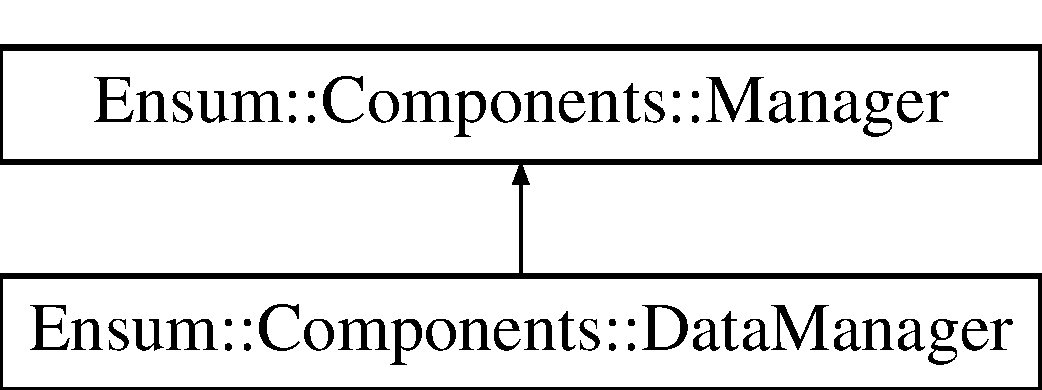
\includegraphics[height=2.000000cm]{class_ensum_1_1_components_1_1_data_manager}
\end{center}
\end{figure}
\subsection*{Classes}
\begin{DoxyCompactItemize}
\item 
struct \hyperlink{struct_ensum_1_1_components_1_1_data_manager_1_1_data}{Data}
\begin{DoxyCompactList}\small\item\em A data struct used for indexing the strings and other growing datatypes in the value\+\_\+buffer. \end{DoxyCompactList}\item 
struct \hyperlink{struct_ensum_1_1_components_1_1_data_manager_1_1_data_buffer}{Data\+Buffer}
\begin{DoxyCompactList}\small\item\em Struct for keeping track of the data entries a entity has been given. \end{DoxyCompactList}\item 
struct \hyperlink{struct_ensum_1_1_components_1_1_data_manager_1_1_entity_data}{Entity\+Data}
\begin{DoxyCompactList}\small\item\em The managers data struct. \end{DoxyCompactList}\item 
struct \hyperlink{struct_ensum_1_1_components_1_1_data_manager_1_1_entry_header}{Entry\+Header}
\begin{DoxyCompactList}\small\item\em The header struct, used for keeping track of the data entries a entity has. \end{DoxyCompactList}\item 
struct \hyperlink{struct_ensum_1_1_components_1_1_data_manager_1_1_value}{Value}
\begin{DoxyCompactList}\small\item\em The value struct, this is where the data is stored. \end{DoxyCompactList}\item 
struct \hyperlink{struct_ensum_1_1_components_1_1_data_manager_1_1_value___buffer}{Value\+\_\+\+Buffer}
\begin{DoxyCompactList}\small\item\em Points to the next free spot in the value\+\_\+buffer. \end{DoxyCompactList}\end{DoxyCompactItemize}
\subsection*{Public Member Functions}
\begin{DoxyCompactItemize}
\item 
{\bfseries Data\+Manager} (\hyperlink{class_ensum_1_1_components_1_1_entity_manager}{Entity\+Manager} \&ent\+Manager)\hypertarget{class_ensum_1_1_components_1_1_data_manager_ad388bb6d19c8eaca2d7c1fbfc3c2a889}{}\label{class_ensum_1_1_components_1_1_data_manager_ad388bb6d19c8eaca2d7c1fbfc3c2a889}

\item 
const void \hyperlink{class_ensum_1_1_components_1_1_data_manager_ade29bf76080dd342aba5e559fdba012e}{Create\+Data} (const \hyperlink{struct_ensum_1_1_components_1_1_entity}{Entity} \&entity)\hypertarget{class_ensum_1_1_components_1_1_data_manager_ade29bf76080dd342aba5e559fdba012e}{}\label{class_ensum_1_1_components_1_1_data_manager_ade29bf76080dd342aba5e559fdba012e}

\begin{DoxyCompactList}\small\item\em Create the data component for the entity. \end{DoxyCompactList}\item 
const void \hyperlink{class_ensum_1_1_components_1_1_data_manager_a9564b3867e85330db4e6b7b78d81645a}{Add\+Bool\+Value} (const \hyperlink{struct_ensum_1_1_components_1_1_entity}{Entity} \&entity, const \hyperlink{class_ensum_1_1string}{string} \&key, const bool val)\hypertarget{class_ensum_1_1_components_1_1_data_manager_a9564b3867e85330db4e6b7b78d81645a}{}\label{class_ensum_1_1_components_1_1_data_manager_a9564b3867e85330db4e6b7b78d81645a}

\begin{DoxyCompactList}\small\item\em Add the bool value to the given entity and key. \end{DoxyCompactList}\item 
const void \hyperlink{class_ensum_1_1_components_1_1_data_manager_afba14ae03a656e9aa5918fac195d479c}{Add\+Float\+Value} (const \hyperlink{struct_ensum_1_1_components_1_1_entity}{Entity} \&entity, const \hyperlink{class_ensum_1_1string}{string} \&key, const float val)\hypertarget{class_ensum_1_1_components_1_1_data_manager_afba14ae03a656e9aa5918fac195d479c}{}\label{class_ensum_1_1_components_1_1_data_manager_afba14ae03a656e9aa5918fac195d479c}

\begin{DoxyCompactList}\small\item\em Add the float value to the given entity and key. \end{DoxyCompactList}\item 
const void \hyperlink{class_ensum_1_1_components_1_1_data_manager_a0916658dd49bbf814965bfce50767906}{Add\+String\+Value} (const \hyperlink{struct_ensum_1_1_components_1_1_entity}{Entity} \&entity, const \hyperlink{class_ensum_1_1string}{string} \&key, const \hyperlink{class_ensum_1_1string}{string} \&val)\hypertarget{class_ensum_1_1_components_1_1_data_manager_a0916658dd49bbf814965bfce50767906}{}\label{class_ensum_1_1_components_1_1_data_manager_a0916658dd49bbf814965bfce50767906}

\begin{DoxyCompactList}\small\item\em Add the string value to the given entity and key. \end{DoxyCompactList}\item 
const void \hyperlink{class_ensum_1_1_components_1_1_data_manager_a2ef6ead291f631e756b19971e1391acf}{Set\+Bool\+Value} (const \hyperlink{struct_ensum_1_1_components_1_1_entity}{Entity} \&entity, const \hyperlink{class_ensum_1_1string}{string} \&key, const bool val)\hypertarget{class_ensum_1_1_components_1_1_data_manager_a2ef6ead291f631e756b19971e1391acf}{}\label{class_ensum_1_1_components_1_1_data_manager_a2ef6ead291f631e756b19971e1391acf}

\begin{DoxyCompactList}\small\item\em Set the bool value to the given entity and key. \end{DoxyCompactList}\item 
const void \hyperlink{class_ensum_1_1_components_1_1_data_manager_aecdd69439279eb2f1fb68250085ffc3a}{Set\+Float\+Value} (const \hyperlink{struct_ensum_1_1_components_1_1_entity}{Entity} \&entity, const \hyperlink{class_ensum_1_1string}{string} \&key, const float val)\hypertarget{class_ensum_1_1_components_1_1_data_manager_aecdd69439279eb2f1fb68250085ffc3a}{}\label{class_ensum_1_1_components_1_1_data_manager_aecdd69439279eb2f1fb68250085ffc3a}

\begin{DoxyCompactList}\small\item\em Set the float value to the given entity and key. \end{DoxyCompactList}\item 
const void \hyperlink{class_ensum_1_1_components_1_1_data_manager_a97f2560a6bfd6da8c7708737680f8607}{Set\+String\+Value} (const \hyperlink{struct_ensum_1_1_components_1_1_entity}{Entity} \&entity, const \hyperlink{class_ensum_1_1string}{string} \&key, const \hyperlink{class_ensum_1_1string}{string} \&val)\hypertarget{class_ensum_1_1_components_1_1_data_manager_a97f2560a6bfd6da8c7708737680f8607}{}\label{class_ensum_1_1_components_1_1_data_manager_a97f2560a6bfd6da8c7708737680f8607}

\begin{DoxyCompactList}\small\item\em Set the string value to the given entity and key. \end{DoxyCompactList}\item 
bool \hyperlink{class_ensum_1_1_components_1_1_data_manager_a1746cbced0b28fc0f4d09097f91e7959}{Get\+Bool\+Value} (const \hyperlink{struct_ensum_1_1_components_1_1_entity}{Entity} \&entity, const \hyperlink{class_ensum_1_1string}{string} \&key)\hypertarget{class_ensum_1_1_components_1_1_data_manager_a1746cbced0b28fc0f4d09097f91e7959}{}\label{class_ensum_1_1_components_1_1_data_manager_a1746cbced0b28fc0f4d09097f91e7959}

\begin{DoxyCompactList}\small\item\em Get the bool value to the given entity and key. \end{DoxyCompactList}\item 
float \hyperlink{class_ensum_1_1_components_1_1_data_manager_a47c2d9326214b16167d455f03a3473de}{Get\+Float\+Value} (const \hyperlink{struct_ensum_1_1_components_1_1_entity}{Entity} \&entity, const \hyperlink{class_ensum_1_1string}{string} \&key)\hypertarget{class_ensum_1_1_components_1_1_data_manager_a47c2d9326214b16167d455f03a3473de}{}\label{class_ensum_1_1_components_1_1_data_manager_a47c2d9326214b16167d455f03a3473de}

\begin{DoxyCompactList}\small\item\em Get the float value to the given entity and key. \end{DoxyCompactList}\item 
\hyperlink{class_ensum_1_1string}{string} \hyperlink{class_ensum_1_1_components_1_1_data_manager_ac7cd482c2e9aa4f1f88cc64301fa5b6b}{Get\+String\+Value} (const \hyperlink{struct_ensum_1_1_components_1_1_entity}{Entity} \&entity, const \hyperlink{class_ensum_1_1string}{string} \&key)\hypertarget{class_ensum_1_1_components_1_1_data_manager_ac7cd482c2e9aa4f1f88cc64301fa5b6b}{}\label{class_ensum_1_1_components_1_1_data_manager_ac7cd482c2e9aa4f1f88cc64301fa5b6b}

\begin{DoxyCompactList}\small\item\em Get the string value to the given entity and key. \end{DoxyCompactList}\end{DoxyCompactItemize}
\subsection*{Private Types}
\begin{DoxyCompactItemize}
\item 
enum \hyperlink{class_ensum_1_1_components_1_1_data_manager_abf17780149860893e39b561e1d98e1e2}{Data\+Type} \+: uint32\+\_\+t \{ {\bfseries B\+O\+OL}, 
{\bfseries F\+L\+O\+AT}, 
{\bfseries S\+T\+R\+I\+NG}
 \}\hypertarget{class_ensum_1_1_components_1_1_data_manager_abf17780149860893e39b561e1d98e1e2}{}\label{class_ensum_1_1_components_1_1_data_manager_abf17780149860893e39b561e1d98e1e2}
\begin{DoxyCompactList}\small\item\em enum class for the kinds of data that can be stored as an entry. \end{DoxyCompactList}
\end{DoxyCompactItemize}
\subsection*{Private Member Functions}
\begin{DoxyCompactItemize}
\item 
const void \hyperlink{class_ensum_1_1_components_1_1_data_manager_aa9f344da59b7fda790b79a9e453ba7c4}{\+\_\+\+Allocate} (uint32\+\_\+t size)
\begin{DoxyCompactList}\small\item\em Allocate more memory. \end{DoxyCompactList}\item 
const void \hyperlink{class_ensum_1_1_components_1_1_data_manager_a6f5c2ed92eba2cb4d5c15c451cbf089c}{\+\_\+\+Destroy} (uint32\+\_\+t index)
\begin{DoxyCompactList}\small\item\em Delete an entry in the memory block. \end{DoxyCompactList}\end{DoxyCompactItemize}
\subsection*{Private Attributes}
\begin{DoxyCompactItemize}
\item 
\hyperlink{struct_ensum_1_1_components_1_1_data_manager_1_1_entity_data}{Entity\+Data} $\ast$ \hyperlink{class_ensum_1_1_components_1_1_data_manager_a03fb52e21fcfdf08e9dd11a71da74385}{\+\_\+datap}
\end{DoxyCompactItemize}
\subsection*{Additional Inherited Members}


\subsection{Member Function Documentation}
\index{Ensum\+::\+Components\+::\+Data\+Manager@{Ensum\+::\+Components\+::\+Data\+Manager}!\+\_\+\+Allocate@{\+\_\+\+Allocate}}
\index{\+\_\+\+Allocate@{\+\_\+\+Allocate}!Ensum\+::\+Components\+::\+Data\+Manager@{Ensum\+::\+Components\+::\+Data\+Manager}}
\subsubsection[{\texorpdfstring{\+\_\+\+Allocate(uint32\+\_\+t size)}{_Allocate(uint32_t size)}}]{\setlength{\rightskip}{0pt plus 5cm}const void Ensum\+::\+Components\+::\+Data\+Manager\+::\+\_\+\+Allocate (
\begin{DoxyParamCaption}
\item[{uint32\+\_\+t}]{size}
\end{DoxyParamCaption}
)\hspace{0.3cm}{\ttfamily [private]}, {\ttfamily [virtual]}}\hypertarget{class_ensum_1_1_components_1_1_data_manager_aa9f344da59b7fda790b79a9e453ba7c4}{}\label{class_ensum_1_1_components_1_1_data_manager_aa9f344da59b7fda790b79a9e453ba7c4}


Allocate more memory. 



Implements \hyperlink{class_ensum_1_1_components_1_1_manager_a1b593059210d09632c910a6abaae49c0}{Ensum\+::\+Components\+::\+Manager}.

\index{Ensum\+::\+Components\+::\+Data\+Manager@{Ensum\+::\+Components\+::\+Data\+Manager}!\+\_\+\+Destroy@{\+\_\+\+Destroy}}
\index{\+\_\+\+Destroy@{\+\_\+\+Destroy}!Ensum\+::\+Components\+::\+Data\+Manager@{Ensum\+::\+Components\+::\+Data\+Manager}}
\subsubsection[{\texorpdfstring{\+\_\+\+Destroy(uint32\+\_\+t index)}{_Destroy(uint32_t index)}}]{\setlength{\rightskip}{0pt plus 5cm}const void Ensum\+::\+Components\+::\+Data\+Manager\+::\+\_\+\+Destroy (
\begin{DoxyParamCaption}
\item[{uint32\+\_\+t}]{index}
\end{DoxyParamCaption}
)\hspace{0.3cm}{\ttfamily [private]}, {\ttfamily [virtual]}}\hypertarget{class_ensum_1_1_components_1_1_data_manager_a6f5c2ed92eba2cb4d5c15c451cbf089c}{}\label{class_ensum_1_1_components_1_1_data_manager_a6f5c2ed92eba2cb4d5c15c451cbf089c}


Delete an entry in the memory block. 

The deleted entry is replaced by the last in the block. 

Implements \hyperlink{class_ensum_1_1_components_1_1_manager_a5ba85395802e942ed8904ca18951e6b0}{Ensum\+::\+Components\+::\+Manager}.



\subsection{Member Data Documentation}
\index{Ensum\+::\+Components\+::\+Data\+Manager@{Ensum\+::\+Components\+::\+Data\+Manager}!\+\_\+datap@{\+\_\+datap}}
\index{\+\_\+datap@{\+\_\+datap}!Ensum\+::\+Components\+::\+Data\+Manager@{Ensum\+::\+Components\+::\+Data\+Manager}}
\subsubsection[{\texorpdfstring{\+\_\+datap}{_datap}}]{\setlength{\rightskip}{0pt plus 5cm}{\bf Entity\+Data}$\ast$ Ensum\+::\+Components\+::\+Data\+Manager\+::\+\_\+datap\hspace{0.3cm}{\ttfamily [private]}}\hypertarget{class_ensum_1_1_components_1_1_data_manager_a03fb52e21fcfdf08e9dd11a71da74385}{}\label{class_ensum_1_1_components_1_1_data_manager_a03fb52e21fcfdf08e9dd11a71da74385}
A reference pointer to avoid having to cast the basic datapointer all the time. 

The documentation for this class was generated from the following file\+:\begin{DoxyCompactItemize}
\item 
Includes/\+Ensum\+\_\+components/Data\+Manager.\+h\end{DoxyCompactItemize}

\hypertarget{class_ensum_1_1_delegate}{}\section{Ensum\+:\+:Delegate$<$ T $>$ Class Template Reference}
\label{class_ensum_1_1_delegate}\index{Ensum\+::\+Delegate$<$ T $>$@{Ensum\+::\+Delegate$<$ T $>$}}


What is this file? A delegate class that can be used to pass free functions or member functions to an event.  




{\ttfamily \#include $<$Event.\+h$>$}



\subsection{Detailed Description}
\subsubsection*{template$<$typename T$>$\\*
class Ensum\+::\+Delegate$<$ T $>$}

What is this file? A delegate class that can be used to pass free functions or member functions to an event. 

See more at \href{http://www.codeproject.com/Articles/11015/The-Impossibly-Fast-C-Delegates}{\tt http\+://www.\+codeproject.\+com/\+Articles/11015/\+The-\/\+Impossibly-\/\+Fast-\/\+C-\/\+Delegates} There doesn\textquotesingle{}t seem to exist a much simpler way. std\+::function was considered, but due to lack of an equality operator they cannot be compared, ergo they also cannot be unsubscribed. Game Coding Complete says that C\#-\/style events would be nice, but C++ doesn\textquotesingle{}t support them out of the box. They do note however that it can be done using alot of template magic, with emphasis on alot. This solution works, but the syntax is horrible.

The event itself is just a collection of delegates that should be called when the event occurs. Triggering the event is done by the one owning the event. 

The documentation for this class was generated from the following file\+:\begin{DoxyCompactItemize}
\item 
C\+:/\+Users/peter/\+Source/\+Repos/\+E\+N\+S\+U\+M/\+Ensum/\+Includes/Event.\+h\end{DoxyCompactItemize}

\hypertarget{class_ensum_1_1_delegate_3_01_return_type_07_param_types_8_8_8_08_4}{}\section{Ensum\+:\+:Delegate$<$ Return\+Type(Param\+Types...)$>$ Class Template Reference}
\label{class_ensum_1_1_delegate_3_01_return_type_07_param_types_8_8_8_08_4}\index{Ensum\+::\+Delegate$<$ Return\+Type(\+Param\+Types...)$>$@{Ensum\+::\+Delegate$<$ Return\+Type(\+Param\+Types...)$>$}}


What is this file? A delegate class that can be used to pass free functions or member functions to an event.  




{\ttfamily \#include $<$Event.\+h$>$}

\subsection*{Public Member Functions}
\begin{DoxyCompactItemize}
\item 
{\bfseries Delegate} (void $\ast$callee, Type function)\hypertarget{class_ensum_1_1_delegate_3_01_return_type_07_param_types_8_8_8_08_4_a14209a13cac7a23f8c2a1aec5fff1534}{}\label{class_ensum_1_1_delegate_3_01_return_type_07_param_types_8_8_8_08_4_a14209a13cac7a23f8c2a1aec5fff1534}

\item 
Return\+Type {\bfseries operator()} (Param\+Types...\+x) const \hypertarget{class_ensum_1_1_delegate_3_01_return_type_07_param_types_8_8_8_08_4_ab92a4899a8fa0166e3c5d6888ebd2413}{}\label{class_ensum_1_1_delegate_3_01_return_type_07_param_types_8_8_8_08_4_ab92a4899a8fa0166e3c5d6888ebd2413}

\item 
bool {\bfseries operator==} (const \hyperlink{class_ensum_1_1_delegate}{Delegate} \&other) const \hypertarget{class_ensum_1_1_delegate_3_01_return_type_07_param_types_8_8_8_08_4_a164df402bddec2eea14b2fb47c121de9}{}\label{class_ensum_1_1_delegate_3_01_return_type_07_param_types_8_8_8_08_4_a164df402bddec2eea14b2fb47c121de9}

\end{DoxyCompactItemize}
\subsection*{Static Public Member Functions}
\begin{DoxyCompactItemize}
\item 
{\footnotesize template$<$class T , Return\+Type(\+T\+::$\ast$)(\+Param\+Types...) T\+Method$>$ }\\static \hyperlink{class_ensum_1_1_delegate}{Delegate} {\bfseries Make} (T $\ast$callee)\hypertarget{class_ensum_1_1_delegate_3_01_return_type_07_param_types_8_8_8_08_4_a33d5bd259c40a08b2ac401a0552162e1}{}\label{class_ensum_1_1_delegate_3_01_return_type_07_param_types_8_8_8_08_4_a33d5bd259c40a08b2ac401a0552162e1}

\item 
{\footnotesize template$<$Return\+Type($\ast$)(\+Param\+Types...) func\+Ptr$>$ }\\static \hyperlink{class_ensum_1_1_delegate}{Delegate} {\bfseries Make} ()\hypertarget{class_ensum_1_1_delegate_3_01_return_type_07_param_types_8_8_8_08_4_afc8561e5caf8588aedcfc954aa1eea89}{}\label{class_ensum_1_1_delegate_3_01_return_type_07_param_types_8_8_8_08_4_afc8561e5caf8588aedcfc954aa1eea89}

\end{DoxyCompactItemize}
\subsection*{Private Types}
\begin{DoxyCompactItemize}
\item 
typedef Return\+Type($\ast$ {\bfseries Type}) (void $\ast$callee, Param\+Types...)\hypertarget{class_ensum_1_1_delegate_3_01_return_type_07_param_types_8_8_8_08_4_a5503bf2523d8be839ac47fdb49946f37}{}\label{class_ensum_1_1_delegate_3_01_return_type_07_param_types_8_8_8_08_4_a5503bf2523d8be839ac47fdb49946f37}

\end{DoxyCompactItemize}
\subsection*{Static Private Member Functions}
\begin{DoxyCompactItemize}
\item 
{\footnotesize template$<$class T , Return\+Type(\+T\+::$\ast$)(\+Param\+Types...) T\+Method$>$ }\\static Return\+Type {\bfseries method\+Caller} (void $\ast$callee, Param\+Types...\+x)\hypertarget{class_ensum_1_1_delegate_3_01_return_type_07_param_types_8_8_8_08_4_ad80559b29464429d6c5b154dafc8a55f}{}\label{class_ensum_1_1_delegate_3_01_return_type_07_param_types_8_8_8_08_4_ad80559b29464429d6c5b154dafc8a55f}

\item 
{\footnotesize template$<$Return\+Type($\ast$)(\+Param\+Types...) func$>$ }\\static Return\+Type {\bfseries function\+Caller} (void $\ast$unused, Param\+Types...\+x)\hypertarget{class_ensum_1_1_delegate_3_01_return_type_07_param_types_8_8_8_08_4_a5f7d20d29a86b79fa56179802df350c3}{}\label{class_ensum_1_1_delegate_3_01_return_type_07_param_types_8_8_8_08_4_a5f7d20d29a86b79fa56179802df350c3}

\end{DoxyCompactItemize}
\subsection*{Private Attributes}
\begin{DoxyCompactItemize}
\item 
void $\ast$ {\bfseries \+\_\+callee}\hypertarget{class_ensum_1_1_delegate_3_01_return_type_07_param_types_8_8_8_08_4_a544eff1d37dad61b5d62520a967f9685}{}\label{class_ensum_1_1_delegate_3_01_return_type_07_param_types_8_8_8_08_4_a544eff1d37dad61b5d62520a967f9685}

\item 
Type {\bfseries \+\_\+callback\+Function}\hypertarget{class_ensum_1_1_delegate_3_01_return_type_07_param_types_8_8_8_08_4_a24614e76a613f902e377ddacaa4d74a7}{}\label{class_ensum_1_1_delegate_3_01_return_type_07_param_types_8_8_8_08_4_a24614e76a613f902e377ddacaa4d74a7}

\end{DoxyCompactItemize}


\subsection{Detailed Description}
\subsubsection*{template$<$typename Return\+Type, typename... Param\+Types$>$\\*
class Ensum\+::\+Delegate$<$ Return\+Type(\+Param\+Types...)$>$}

What is this file? A delegate class that can be used to pass free functions or member functions to an event. 

See more at \href{http://www.codeproject.com/Articles/11015/The-Impossibly-Fast-C-Delegates}{\tt http\+://www.\+codeproject.\+com/\+Articles/11015/\+The-\/\+Impossibly-\/\+Fast-\/\+C-\/\+Delegates} There doesn\textquotesingle{}t seem to exist a much simpler way. std\+::function was considered, but due to lack of an equality operator they cannot be compared, ergo they also cannot be unsubscribed. Game Coding Complete says that C\#-\/style events would be nice, but C++ doesn\textquotesingle{}t support them out of the box. They do note however that it can be done using alot of template magic, with emphasis on alot. This solution works, but the syntax is horrible.

The event itself is just a collection of delegates that should be called when the event occurs. Triggering the event is done by the one owning the event. 

The documentation for this class was generated from the following file\+:\begin{DoxyCompactItemize}
\item 
Includes/Event.\+h\end{DoxyCompactItemize}

\hypertarget{struct_ensum_1_1_graphics_1_1_depth_buffer}{}\section{Ensum\+:\+:Graphics\+:\+:Depth\+Buffer Struct Reference}
\label{struct_ensum_1_1_graphics_1_1_depth_buffer}\index{Ensum\+::\+Graphics\+::\+Depth\+Buffer@{Ensum\+::\+Graphics\+::\+Depth\+Buffer}}
\subsection*{Public Attributes}
\begin{DoxyCompactItemize}
\item 
I\+D3\+D11\+Resource $\ast$ {\bfseries Texture} = nullptr\hypertarget{struct_ensum_1_1_graphics_1_1_depth_buffer_a5cdab429ed3f314664397b7c22ad9cb0}{}\label{struct_ensum_1_1_graphics_1_1_depth_buffer_a5cdab429ed3f314664397b7c22ad9cb0}

\item 
I\+D3\+D11\+Depth\+Stencil\+View $\ast$ {\bfseries D\+SV} = nullptr\hypertarget{struct_ensum_1_1_graphics_1_1_depth_buffer_a814cdc40ae92b5c3eeeb357891409570}{}\label{struct_ensum_1_1_graphics_1_1_depth_buffer_a814cdc40ae92b5c3eeeb357891409570}

\item 
I\+D3\+D11\+Depth\+Stencil\+View $\ast$ {\bfseries D\+S\+V\+Read\+Only} = nullptr\hypertarget{struct_ensum_1_1_graphics_1_1_depth_buffer_af0725e42b872cf226376dd95a40d5be4}{}\label{struct_ensum_1_1_graphics_1_1_depth_buffer_af0725e42b872cf226376dd95a40d5be4}

\item 
I\+D3\+D11\+Shader\+Resource\+View $\ast$ {\bfseries S\+RV} = nullptr\hypertarget{struct_ensum_1_1_graphics_1_1_depth_buffer_a3b850a6be4b660aeb516db7d4dd766ba}{}\label{struct_ensum_1_1_graphics_1_1_depth_buffer_a3b850a6be4b660aeb516db7d4dd766ba}

\item 
I\+D3\+D11\+Depth\+Stencil\+View $\ast$$\ast$ {\bfseries D\+S\+V\+Slices} = nullptr\hypertarget{struct_ensum_1_1_graphics_1_1_depth_buffer_a77e80fa29a60d70965b88c856b7168e2}{}\label{struct_ensum_1_1_graphics_1_1_depth_buffer_a77e80fa29a60d70965b88c856b7168e2}

\item 
I\+D3\+D11\+Depth\+Stencil\+View $\ast$$\ast$ {\bfseries D\+S\+V\+Read\+Only\+Slices} = nullptr\hypertarget{struct_ensum_1_1_graphics_1_1_depth_buffer_a1fc14b666064c66af03b00166212c12a}{}\label{struct_ensum_1_1_graphics_1_1_depth_buffer_a1fc14b666064c66af03b00166212c12a}

\item 
I\+D3\+D11\+Shader\+Resource\+View $\ast$$\ast$ {\bfseries S\+R\+V\+Slices} = nullptr\hypertarget{struct_ensum_1_1_graphics_1_1_depth_buffer_a58d957a868984e88f907295381c8a765}{}\label{struct_ensum_1_1_graphics_1_1_depth_buffer_a58d957a868984e88f907295381c8a765}

\item 
unsigned {\bfseries Slice\+Count} = 1\hypertarget{struct_ensum_1_1_graphics_1_1_depth_buffer_a01031a04589167914241edce0ff6b789}{}\label{struct_ensum_1_1_graphics_1_1_depth_buffer_a01031a04589167914241edce0ff6b789}

\item 
D\+X\+G\+I\+\_\+\+F\+O\+R\+M\+AT {\bfseries Format\+Tex} = D\+X\+G\+I\+\_\+\+F\+O\+R\+M\+A\+T\+\_\+\+U\+N\+K\+N\+O\+WN\hypertarget{struct_ensum_1_1_graphics_1_1_depth_buffer_a9a6f1b6a7b51a76d5337a66c3a47d35f}{}\label{struct_ensum_1_1_graphics_1_1_depth_buffer_a9a6f1b6a7b51a76d5337a66c3a47d35f}

\item 
D\+X\+G\+I\+\_\+\+F\+O\+R\+M\+AT {\bfseries Format\+D\+SV} = D\+X\+G\+I\+\_\+\+F\+O\+R\+M\+A\+T\+\_\+\+U\+N\+K\+N\+O\+WN\hypertarget{struct_ensum_1_1_graphics_1_1_depth_buffer_ac5d3bfd41369491752b31837fdd35f5d}{}\label{struct_ensum_1_1_graphics_1_1_depth_buffer_ac5d3bfd41369491752b31837fdd35f5d}

\item 
D\+X\+G\+I\+\_\+\+F\+O\+R\+M\+AT {\bfseries Format\+S\+RV} = D\+X\+G\+I\+\_\+\+F\+O\+R\+M\+A\+T\+\_\+\+U\+N\+K\+N\+O\+WN\hypertarget{struct_ensum_1_1_graphics_1_1_depth_buffer_a1aa719dc13932e0369bac8d9d173378b}{}\label{struct_ensum_1_1_graphics_1_1_depth_buffer_a1aa719dc13932e0369bac8d9d173378b}

\item 
unsigned {\bfseries Width} = 0\hypertarget{struct_ensum_1_1_graphics_1_1_depth_buffer_ad14c64afb64df36540822bc7a433df94}{}\label{struct_ensum_1_1_graphics_1_1_depth_buffer_ad14c64afb64df36540822bc7a433df94}

\item 
unsigned {\bfseries Height} = 0\hypertarget{struct_ensum_1_1_graphics_1_1_depth_buffer_af2a5169f76b3d27442051d34d69212db}{}\label{struct_ensum_1_1_graphics_1_1_depth_buffer_af2a5169f76b3d27442051d34d69212db}

\item 
unsigned {\bfseries Array\+Size} = 1\hypertarget{struct_ensum_1_1_graphics_1_1_depth_buffer_a3e39d22a9b572cf5156b06fbdc439c93}{}\label{struct_ensum_1_1_graphics_1_1_depth_buffer_a3e39d22a9b572cf5156b06fbdc439c93}

\item 
unsigned {\bfseries Mip\+Levels} = 1\hypertarget{struct_ensum_1_1_graphics_1_1_depth_buffer_ad19eb78fd05249659dbbc5b980ca65a6}{}\label{struct_ensum_1_1_graphics_1_1_depth_buffer_ad19eb78fd05249659dbbc5b980ca65a6}

\item 
unsigned {\bfseries Sample\+Count} = 1\hypertarget{struct_ensum_1_1_graphics_1_1_depth_buffer_a790fb691f3e42bc0fdf1daeea85227ea}{}\label{struct_ensum_1_1_graphics_1_1_depth_buffer_a790fb691f3e42bc0fdf1daeea85227ea}

\end{DoxyCompactItemize}


The documentation for this struct was generated from the following file\+:\begin{DoxyCompactItemize}
\item 
C\+:/\+Users/peter/\+Source/\+Repos/\+E\+N\+S\+U\+M/\+Ensum/\+Includes/\+Ensum\+\_\+graphics/Direct3\+D11.\+h\end{DoxyCompactItemize}

\hypertarget{struct_ensum_1_1_graphics_1_1_depth_stencil_state}{}\section{Ensum\+:\+:Graphics\+:\+:Depth\+Stencil\+State Struct Reference}
\label{struct_ensum_1_1_graphics_1_1_depth_stencil_state}\index{Ensum\+::\+Graphics\+::\+Depth\+Stencil\+State@{Ensum\+::\+Graphics\+::\+Depth\+Stencil\+State}}
\subsection*{Public Attributes}
\begin{DoxyCompactItemize}
\item 
I\+D3\+D11\+Depth\+Stencil\+State $\ast$ {\bfseries D\+SS} = nullptr\hypertarget{struct_ensum_1_1_graphics_1_1_depth_stencil_state_a0eda3ff24b49370c55ebac4e4005e9e3}{}\label{struct_ensum_1_1_graphics_1_1_depth_stencil_state_a0eda3ff24b49370c55ebac4e4005e9e3}

\item 
bool {\bfseries depth\+Enable} = true\hypertarget{struct_ensum_1_1_graphics_1_1_depth_stencil_state_afe7a1623a3c1bf7c4843d7e0d911b109}{}\label{struct_ensum_1_1_graphics_1_1_depth_stencil_state_afe7a1623a3c1bf7c4843d7e0d911b109}

\item 
D3\+D11\+\_\+\+D\+E\+P\+T\+H\+\_\+\+W\+R\+I\+T\+E\+\_\+\+M\+A\+SK {\bfseries depth\+Write\+Mask} = D3\+D11\+\_\+\+D\+E\+P\+T\+H\+\_\+\+W\+R\+I\+T\+E\+\_\+\+M\+A\+S\+K\+\_\+\+A\+LL\hypertarget{struct_ensum_1_1_graphics_1_1_depth_stencil_state_a688b85ba9c0577fe39aac432d9d78b16}{}\label{struct_ensum_1_1_graphics_1_1_depth_stencil_state_a688b85ba9c0577fe39aac432d9d78b16}

\item 
D3\+D11\+\_\+\+C\+O\+M\+P\+A\+R\+I\+S\+O\+N\+\_\+\+F\+U\+NC {\bfseries depth\+Comparison} = D3\+D11\+\_\+\+C\+O\+M\+P\+A\+R\+I\+S\+O\+N\+\_\+\+L\+E\+SS\hypertarget{struct_ensum_1_1_graphics_1_1_depth_stencil_state_a1a550c0d390f87b4571a2dd0f807d5bb}{}\label{struct_ensum_1_1_graphics_1_1_depth_stencil_state_a1a550c0d390f87b4571a2dd0f807d5bb}

\item 
bool {\bfseries stencil\+Enable} = false\hypertarget{struct_ensum_1_1_graphics_1_1_depth_stencil_state_a4130e5ac3b4651eeb059c39805eff89e}{}\label{struct_ensum_1_1_graphics_1_1_depth_stencil_state_a4130e5ac3b4651eeb059c39805eff89e}

\item 
U\+I\+N\+T8 {\bfseries stencil\+Read\+Mask} = 0x\+FF\hypertarget{struct_ensum_1_1_graphics_1_1_depth_stencil_state_aecd3bef478e6e09e8fb922bfa7da6b6c}{}\label{struct_ensum_1_1_graphics_1_1_depth_stencil_state_aecd3bef478e6e09e8fb922bfa7da6b6c}

\item 
U\+I\+N\+T8 {\bfseries stencil\+Write\+Mask} = 0x\+FF\hypertarget{struct_ensum_1_1_graphics_1_1_depth_stencil_state_a0627f6674b5c6fc32d0e0d0ffb8551f1}{}\label{struct_ensum_1_1_graphics_1_1_depth_stencil_state_a0627f6674b5c6fc32d0e0d0ffb8551f1}

\end{DoxyCompactItemize}


The documentation for this struct was generated from the following file\+:\begin{DoxyCompactItemize}
\item 
C\+:/\+Users/peter/\+Source/\+Repos/\+E\+N\+S\+U\+M/\+Ensum/\+Includes/\+Ensum\+\_\+graphics/Direct3\+D11.\+h\end{DoxyCompactItemize}

\hypertarget{class_ensum_1_1_graphics_1_1_direct3_d11}{}\section{Ensum\+:\+:Graphics\+:\+:Direct3\+D11 Class Reference}
\label{class_ensum_1_1_graphics_1_1_direct3_d11}\index{Ensum\+::\+Graphics\+::\+Direct3\+D11@{Ensum\+::\+Graphics\+::\+Direct3\+D11}}
\subsection*{Public Member Functions}
\begin{DoxyCompactItemize}
\item 
const void {\bfseries Start} ()\hypertarget{class_ensum_1_1_graphics_1_1_direct3_d11_a12b3a76ee7552796aef3385222a79c7b}{}\label{class_ensum_1_1_graphics_1_1_direct3_d11_a12b3a76ee7552796aef3385222a79c7b}

\item 
const void {\bfseries Shutdown} (void)\hypertarget{class_ensum_1_1_graphics_1_1_direct3_d11_ab8fab874dc6263d67ec4e9bfa0e2991e}{}\label{class_ensum_1_1_graphics_1_1_direct3_d11_ab8fab874dc6263d67ec4e9bfa0e2991e}

\item 
const void {\bfseries Resize} ()\hypertarget{class_ensum_1_1_graphics_1_1_direct3_d11_ac1d1ae70143ca8c795526dad0bf03fe6}{}\label{class_ensum_1_1_graphics_1_1_direct3_d11_ac1d1ae70143ca8c795526dad0bf03fe6}

\item 
I\+D3\+D11\+Device $\ast$ {\bfseries Get\+Device} ()\hypertarget{class_ensum_1_1_graphics_1_1_direct3_d11_a4ba00335d046107496f7bf9decc7f729}{}\label{class_ensum_1_1_graphics_1_1_direct3_d11_a4ba00335d046107496f7bf9decc7f729}

\item 
I\+D3\+D11\+Device\+Context $\ast$ {\bfseries Get\+Device\+Context} ()\hypertarget{class_ensum_1_1_graphics_1_1_direct3_d11_a5be4ad19e4d80399289e89eba6bdeb99}{}\label{class_ensum_1_1_graphics_1_1_direct3_d11_a5be4ad19e4d80399289e89eba6bdeb99}

\item 
I\+D\+X\+G\+I\+Swap\+Chain $\ast$ {\bfseries Get\+Swap\+Chain} ()\hypertarget{class_ensum_1_1_graphics_1_1_direct3_d11_ac022c45da3e0456366b2c99e533fb964}{}\label{class_ensum_1_1_graphics_1_1_direct3_d11_ac022c45da3e0456366b2c99e533fb964}

\item 
I\+D3\+D11\+Render\+Target\+View $\ast$ {\bfseries Get\+Back\+Buffer\+R\+TV} ()\hypertarget{class_ensum_1_1_graphics_1_1_direct3_d11_a03b866538c72558c4e43a7b76a2b1c2e}{}\label{class_ensum_1_1_graphics_1_1_direct3_d11_a03b866538c72558c4e43a7b76a2b1c2e}

\item 
\hyperlink{struct_ensum_1_1_graphics_1_1_render_target}{Render\+Target} {\bfseries Create\+Render\+Target} (D\+X\+G\+I\+\_\+\+F\+O\+R\+M\+AT format, unsigned width, unsigned height, unsigned depth, unsigned flags=0, unsigned array\+Size=1, unsigned mip\+Levels=1, unsigned sample\+Count=1) const \hypertarget{class_ensum_1_1_graphics_1_1_direct3_d11_a1f485443b98ca65ad7cf3a4e7fe8ab01}{}\label{class_ensum_1_1_graphics_1_1_direct3_d11_a1f485443b98ca65ad7cf3a4e7fe8ab01}

\item 
const void {\bfseries Delete\+Render\+Target} (\hyperlink{struct_ensum_1_1_graphics_1_1_render_target}{Render\+Target} \&rt) const \hypertarget{class_ensum_1_1_graphics_1_1_direct3_d11_ae92708638a582ef8f9c1b3365cb13c15}{}\label{class_ensum_1_1_graphics_1_1_direct3_d11_ae92708638a582ef8f9c1b3365cb13c15}

\item 
\hyperlink{struct_ensum_1_1_graphics_1_1_depth_buffer}{Depth\+Buffer} {\bfseries Create\+Depth\+Buffer} (D\+X\+G\+I\+\_\+\+F\+O\+R\+M\+AT format, unsigned width, unsigned height, bool sample\+In\+Shader=false, unsigned flags=0, unsigned array\+Size=1, unsigned mip\+Levels=1, unsigned sample\+Count=1) const \hypertarget{class_ensum_1_1_graphics_1_1_direct3_d11_a92b2f778d29d893b02d2340b5f5fd601}{}\label{class_ensum_1_1_graphics_1_1_direct3_d11_a92b2f778d29d893b02d2340b5f5fd601}

\item 
const void {\bfseries Delete\+Depth\+Buffer} (\hyperlink{struct_ensum_1_1_graphics_1_1_depth_buffer}{Depth\+Buffer} \&db) const \hypertarget{class_ensum_1_1_graphics_1_1_direct3_d11_a59404f3cb164d6f4090fb08ed807a8ba}{}\label{class_ensum_1_1_graphics_1_1_direct3_d11_a59404f3cb164d6f4090fb08ed807a8ba}

\item 
\hyperlink{struct_ensum_1_1_graphics_1_1_structured_buffer}{Structured\+Buffer} {\bfseries Create\+Structured\+Buffer} (unsigned stride, unsigned element\+Count, bool C\+P\+U\+Write=true, bool G\+P\+U\+Write=false, const void $\ast$initial\+Data=nullptr, bool add\+Structure\+Counter=false) const \hypertarget{class_ensum_1_1_graphics_1_1_direct3_d11_a817c74a8413dc1786d08c1d9ed8a214d}{}\label{class_ensum_1_1_graphics_1_1_direct3_d11_a817c74a8413dc1786d08c1d9ed8a214d}

\item 
\hyperlink{struct_ensum_1_1_graphics_1_1_structured_buffer}{Structured\+Buffer} {\bfseries Create\+Append\+Consume\+Buffer} (unsigned stride, unsigned element\+Count, const void $\ast$initial\+Data=nullptr) const \hypertarget{class_ensum_1_1_graphics_1_1_direct3_d11_a56d338dff88648277a5f49882b6af286}{}\label{class_ensum_1_1_graphics_1_1_direct3_d11_a56d338dff88648277a5f49882b6af286}

\item 
const void {\bfseries Delete\+Structured\+Buffer} (\hyperlink{struct_ensum_1_1_graphics_1_1_structured_buffer}{Structured\+Buffer} \&sb) const \hypertarget{class_ensum_1_1_graphics_1_1_direct3_d11_a7a6698ae37a063a0ca9bbe6d649fe90f}{}\label{class_ensum_1_1_graphics_1_1_direct3_d11_a7a6698ae37a063a0ca9bbe6d649fe90f}

\item 
\hyperlink{struct_ensum_1_1_graphics_1_1_indirect_args_buffer}{Indirect\+Args\+Buffer} {\bfseries Create\+Indirect\+Args\+Buffer} (unsigned size, void $\ast$initial\+Data=nullptr) const \hypertarget{class_ensum_1_1_graphics_1_1_direct3_d11_aff12bd4ad62cfed85481cabd1f1424e4}{}\label{class_ensum_1_1_graphics_1_1_direct3_d11_aff12bd4ad62cfed85481cabd1f1424e4}

\item 
const void {\bfseries Delete\+Indirect\+Args\+Buffer} (\hyperlink{struct_ensum_1_1_graphics_1_1_indirect_args_buffer}{Indirect\+Args\+Buffer} \&iab) const \hypertarget{class_ensum_1_1_graphics_1_1_direct3_d11_a4daa1cbb069d7380a31080b7fce25d7e}{}\label{class_ensum_1_1_graphics_1_1_direct3_d11_a4daa1cbb069d7380a31080b7fce25d7e}

\item 
\hyperlink{struct_ensum_1_1_graphics_1_1_depth_stencil_state}{Depth\+Stencil\+State} {\bfseries Create\+Depth\+Stencil\+State} (bool depth\+Enable=true, D3\+D11\+\_\+\+D\+E\+P\+T\+H\+\_\+\+W\+R\+I\+T\+E\+\_\+\+M\+A\+SK depth\+Write\+Mask=D3\+D11\+\_\+\+D\+E\+P\+T\+H\+\_\+\+W\+R\+I\+T\+E\+\_\+\+M\+A\+S\+K\+\_\+\+A\+LL, D3\+D11\+\_\+\+C\+O\+M\+P\+A\+R\+I\+S\+O\+N\+\_\+\+F\+U\+NC depth\+Comparison=D3\+D11\+\_\+\+C\+O\+M\+P\+A\+R\+I\+S\+O\+N\+\_\+\+L\+E\+SS, bool stencil\+Enable=false, U\+I\+N\+T8 stencil\+Read\+Mask=0x\+F\+F, U\+I\+N\+T8 stencil\+Write\+Mask=0x\+F\+F) const \hypertarget{class_ensum_1_1_graphics_1_1_direct3_d11_a3202ea5e7bd4ca7b77fc0918e90bc373}{}\label{class_ensum_1_1_graphics_1_1_direct3_d11_a3202ea5e7bd4ca7b77fc0918e90bc373}

\item 
const void {\bfseries Delete\+Depth\+Stencil\+State} (\hyperlink{struct_ensum_1_1_graphics_1_1_depth_stencil_state}{Depth\+Stencil\+State} \&dss) const \hypertarget{class_ensum_1_1_graphics_1_1_direct3_d11_ab90c58cbc32683636eb2657c8787ca57}{}\label{class_ensum_1_1_graphics_1_1_direct3_d11_ab90c58cbc32683636eb2657c8787ca57}

\item 
\hyperlink{struct_ensum_1_1_graphics_1_1_rasterizer_state}{Rasterizer\+State} {\bfseries Create\+Rasterizer\+State} (D3\+D11\+\_\+\+F\+I\+L\+L\+\_\+\+M\+O\+DE fill\+Mode=D3\+D11\+\_\+\+F\+I\+L\+L\+\_\+\+S\+O\+L\+ID, D3\+D11\+\_\+\+C\+U\+L\+L\+\_\+\+M\+O\+DE cull\+Mode=D3\+D11\+\_\+\+C\+U\+L\+L\+\_\+\+B\+A\+CK, bool front\+Counter\+Clockwise=true, bool depth\+Bias=false, float depth\+Bias\+Clamp=0.\+0f, float slope\+Scaled\+Depth\+Bias=0.\+0f, bool depth\+Clip\+Enable=true, bool scissor\+Enable=false, bool multi\+Sample\+Enable=false, bool antialiased\+Line\+Enable=false) const \hypertarget{class_ensum_1_1_graphics_1_1_direct3_d11_a06450d57a4aaf75d607573e202db8558}{}\label{class_ensum_1_1_graphics_1_1_direct3_d11_a06450d57a4aaf75d607573e202db8558}

\item 
const void {\bfseries Delete\+Rasterizer\+State} (\hyperlink{struct_ensum_1_1_graphics_1_1_rasterizer_state}{Rasterizer\+State} \&rs) const \hypertarget{class_ensum_1_1_graphics_1_1_direct3_d11_a51740626ccbd753381c2a2d0120a9b72}{}\label{class_ensum_1_1_graphics_1_1_direct3_d11_a51740626ccbd753381c2a2d0120a9b72}

\item 
\hyperlink{struct_ensum_1_1_graphics_1_1_blend_state}{Blend\+State} {\bfseries Create\+Blend\+State} (bool blend\+Enabled=false, U\+I\+N\+T8 render\+Target\+Write\+Mask=D3\+D11\+\_\+\+C\+O\+L\+O\+R\+\_\+\+W\+R\+I\+T\+E\+\_\+\+E\+N\+A\+B\+L\+E\+\_\+\+A\+LL) const \hypertarget{class_ensum_1_1_graphics_1_1_direct3_d11_ad84a4a23abd2e3c05cdd87955fdbba3d}{}\label{class_ensum_1_1_graphics_1_1_direct3_d11_ad84a4a23abd2e3c05cdd87955fdbba3d}

\item 
\hyperlink{struct_ensum_1_1_graphics_1_1_blend_state}{Blend\+State} {\bfseries Create\+Blend\+State} (D3\+D11\+\_\+\+B\+L\+E\+N\+D\+\_\+\+D\+E\+SC $\ast$blend\+Desc) const \hypertarget{class_ensum_1_1_graphics_1_1_direct3_d11_a60305dc183f6c5994e6d14db88999f94}{}\label{class_ensum_1_1_graphics_1_1_direct3_d11_a60305dc183f6c5994e6d14db88999f94}

\item 
const void {\bfseries Delete\+Blend\+State} (\hyperlink{struct_ensum_1_1_graphics_1_1_blend_state}{Blend\+State} \&bs) const \hypertarget{class_ensum_1_1_graphics_1_1_direct3_d11_a0274aa6937f2da786cdac2f039771f15}{}\label{class_ensum_1_1_graphics_1_1_direct3_d11_a0274aa6937f2da786cdac2f039771f15}

\end{DoxyCompactItemize}
\subsection*{Private Member Functions}
\begin{DoxyCompactItemize}
\item 
{\bfseries Direct3\+D11} (const \hyperlink{class_ensum_1_1_graphics_1_1_direct3_d11}{Direct3\+D11} \&other)\hypertarget{class_ensum_1_1_graphics_1_1_direct3_d11_a7d568c79f32741212046af961492aa68}{}\label{class_ensum_1_1_graphics_1_1_direct3_d11_a7d568c79f32741212046af961492aa68}

\item 
\hyperlink{class_ensum_1_1_graphics_1_1_direct3_d11}{Direct3\+D11} \& {\bfseries operator=} (const \hyperlink{class_ensum_1_1_graphics_1_1_direct3_d11}{Direct3\+D11} \&rhs)\hypertarget{class_ensum_1_1_graphics_1_1_direct3_d11_a557bc6af306005cf46de9d5d0174aec6}{}\label{class_ensum_1_1_graphics_1_1_direct3_d11_a557bc6af306005cf46de9d5d0174aec6}

\item 
I\+D3\+D11\+Render\+Target\+View $\ast$ {\bfseries \+\_\+\+Create\+R\+TV} (I\+D3\+D11\+Resource $\ast$resource, D\+X\+G\+I\+\_\+\+F\+O\+R\+M\+AT format=D\+X\+G\+I\+\_\+\+F\+O\+R\+M\+A\+T\+\_\+\+U\+N\+K\+N\+O\+WN, int first\+Slice=-\/1, unsigned num\+Slices=1) const \hypertarget{class_ensum_1_1_graphics_1_1_direct3_d11_a360fa1814a2e6087c2ba3d0a6018fbcd}{}\label{class_ensum_1_1_graphics_1_1_direct3_d11_a360fa1814a2e6087c2ba3d0a6018fbcd}

\item 
I\+D3\+D11\+Shader\+Resource\+View $\ast$ {\bfseries \+\_\+\+Create\+S\+RV} (I\+D3\+D11\+Resource $\ast$resource, D\+X\+G\+I\+\_\+\+F\+O\+R\+M\+AT format=D\+X\+G\+I\+\_\+\+F\+O\+R\+M\+A\+T\+\_\+\+U\+N\+K\+N\+O\+WN, int first\+Slice=-\/1, unsigned num\+Slices=1) const \hypertarget{class_ensum_1_1_graphics_1_1_direct3_d11_a3b64ff06a76530eaac835d91ca78ceca}{}\label{class_ensum_1_1_graphics_1_1_direct3_d11_a3b64ff06a76530eaac835d91ca78ceca}

\item 
I\+D3\+D11\+Unordered\+Access\+View $\ast$ {\bfseries \+\_\+\+Create\+U\+AV} (I\+D3\+D11\+Resource $\ast$resource, D\+X\+G\+I\+\_\+\+F\+O\+R\+M\+AT format=D\+X\+G\+I\+\_\+\+F\+O\+R\+M\+A\+T\+\_\+\+U\+N\+K\+N\+O\+WN, int first\+Slice=-\/1, unsigned num\+Slices=1) const \hypertarget{class_ensum_1_1_graphics_1_1_direct3_d11_a52387272106b9ef4e7b9be0d0b4fcbc3}{}\label{class_ensum_1_1_graphics_1_1_direct3_d11_a52387272106b9ef4e7b9be0d0b4fcbc3}

\item 
I\+D3\+D11\+Depth\+Stencil\+View $\ast$ {\bfseries \+\_\+\+Create\+D\+SV} (I\+D3\+D11\+Resource $\ast$resource, D\+X\+G\+I\+\_\+\+F\+O\+R\+M\+AT format=D\+X\+G\+I\+\_\+\+F\+O\+R\+M\+A\+T\+\_\+\+U\+N\+K\+N\+O\+WN, bool read\+Only=false, int first\+Slice=-\/1, unsigned num\+Slices=1) const \hypertarget{class_ensum_1_1_graphics_1_1_direct3_d11_a2309142b6f9de0233a05156e0f282eaa}{}\label{class_ensum_1_1_graphics_1_1_direct3_d11_a2309142b6f9de0233a05156e0f282eaa}

\item 
I\+D3\+D11\+Depth\+Stencil\+State $\ast$ {\bfseries \+\_\+\+Create\+D\+SS} (bool depth\+Enable=true, D3\+D11\+\_\+\+D\+E\+P\+T\+H\+\_\+\+W\+R\+I\+T\+E\+\_\+\+M\+A\+SK depth\+Write\+Mask=D3\+D11\+\_\+\+D\+E\+P\+T\+H\+\_\+\+W\+R\+I\+T\+E\+\_\+\+M\+A\+S\+K\+\_\+\+A\+LL, D3\+D11\+\_\+\+C\+O\+M\+P\+A\+R\+I\+S\+O\+N\+\_\+\+F\+U\+NC depth\+Comparison=D3\+D11\+\_\+\+C\+O\+M\+P\+A\+R\+I\+S\+O\+N\+\_\+\+L\+E\+SS, bool stencil\+Enable=false, U\+I\+N\+T8 stencil\+Read\+Mask=0x\+F\+F, U\+I\+N\+T8 stencil\+Write\+Mask=0x\+F\+F) const \hypertarget{class_ensum_1_1_graphics_1_1_direct3_d11_aa6c5d4175898eb21915b1402719d44ee}{}\label{class_ensum_1_1_graphics_1_1_direct3_d11_aa6c5d4175898eb21915b1402719d44ee}

\item 
I\+D3\+D11\+Rasterizer\+State $\ast$ {\bfseries \+\_\+\+Create\+RS} (D3\+D11\+\_\+\+F\+I\+L\+L\+\_\+\+M\+O\+DE fill\+Mode=D3\+D11\+\_\+\+F\+I\+L\+L\+\_\+\+S\+O\+L\+ID, D3\+D11\+\_\+\+C\+U\+L\+L\+\_\+\+M\+O\+DE cull\+Mode=D3\+D11\+\_\+\+C\+U\+L\+L\+\_\+\+B\+A\+CK, bool front\+Counter\+Clockwise=true, bool depth\+Bias=false, float depth\+Bias\+Clamp=0.\+0f, float slope\+Scaled\+Depth\+Bias=0.\+0f, bool depth\+Clip\+Enable=true, bool scissor\+Enable=false, bool multi\+Sample\+Enable=false, bool antialiased\+Line\+Enable=false) const \hypertarget{class_ensum_1_1_graphics_1_1_direct3_d11_a1e93657992eb91b0aa9eaa8d9f96a03e}{}\label{class_ensum_1_1_graphics_1_1_direct3_d11_a1e93657992eb91b0aa9eaa8d9f96a03e}

\item 
I\+D3\+D11\+Blend\+State $\ast$ {\bfseries \+\_\+\+Create\+BS} (bool blend\+Enabled=false, U\+I\+N\+T8 render\+Target\+Write\+Mask=D3\+D11\+\_\+\+C\+O\+L\+O\+R\+\_\+\+W\+R\+I\+T\+E\+\_\+\+E\+N\+A\+B\+L\+E\+\_\+\+A\+LL) const \hypertarget{class_ensum_1_1_graphics_1_1_direct3_d11_a88e514dd663ddcc229a6b61fe6adf19e}{}\label{class_ensum_1_1_graphics_1_1_direct3_d11_a88e514dd663ddcc229a6b61fe6adf19e}

\item 
I\+D3\+D11\+Blend\+State $\ast$ {\bfseries \+\_\+\+Create\+BS} (D3\+D11\+\_\+\+B\+L\+E\+N\+D\+\_\+\+D\+E\+SC $\ast$blend\+Desc) const \hypertarget{class_ensum_1_1_graphics_1_1_direct3_d11_a54184d338e4dd0753ee177eadb726da8}{}\label{class_ensum_1_1_graphics_1_1_direct3_d11_a54184d338e4dd0753ee177eadb726da8}

\end{DoxyCompactItemize}
\subsection*{Private Attributes}
\begin{DoxyCompactItemize}
\item 
H\+W\+ND {\bfseries \+\_\+h\+Wnd}\hypertarget{class_ensum_1_1_graphics_1_1_direct3_d11_ad3fb134a667bf1b31aa6335311c6c874}{}\label{class_ensum_1_1_graphics_1_1_direct3_d11_ad3fb134a667bf1b31aa6335311c6c874}

\item 
I\+D3\+D11\+Device $\ast$ {\bfseries \+\_\+d3d\+Device} = nullptr\hypertarget{class_ensum_1_1_graphics_1_1_direct3_d11_aa6a1333e30d315bd6b2136dd6e23018c}{}\label{class_ensum_1_1_graphics_1_1_direct3_d11_aa6a1333e30d315bd6b2136dd6e23018c}

\item 
I\+D3\+D11\+Device\+Context $\ast$ {\bfseries \+\_\+d3d\+Device\+Context} = nullptr\hypertarget{class_ensum_1_1_graphics_1_1_direct3_d11_ade2ce6e90bff8d33867c4af788702741}{}\label{class_ensum_1_1_graphics_1_1_direct3_d11_ade2ce6e90bff8d33867c4af788702741}

\item 
D3\+D\+\_\+\+F\+E\+A\+T\+U\+R\+E\+\_\+\+L\+E\+V\+EL {\bfseries \+\_\+\+Feature\+Level}\hypertarget{class_ensum_1_1_graphics_1_1_direct3_d11_a82861081b0fedc420c16f0f6c10a201d}{}\label{class_ensum_1_1_graphics_1_1_direct3_d11_a82861081b0fedc420c16f0f6c10a201d}

\item 
I\+D\+X\+G\+I\+Swap\+Chain $\ast$ {\bfseries \+\_\+\+Swap\+Chain} = nullptr\hypertarget{class_ensum_1_1_graphics_1_1_direct3_d11_a0253d19ec8e600ce61c09be8507b40be}{}\label{class_ensum_1_1_graphics_1_1_direct3_d11_a0253d19ec8e600ce61c09be8507b40be}

\item 
I\+D\+X\+G\+I\+Output $\ast$ {\bfseries \+\_\+\+D\+X\+G\+I\+Output} = nullptr\hypertarget{class_ensum_1_1_graphics_1_1_direct3_d11_afd6c2e521b0144834f1ebf76029125eb}{}\label{class_ensum_1_1_graphics_1_1_direct3_d11_afd6c2e521b0144834f1ebf76029125eb}

\item 
I\+D3\+D11\+Render\+Target\+View $\ast$ {\bfseries \+\_\+\+Back\+Buffer\+R\+TV} = nullptr\hypertarget{class_ensum_1_1_graphics_1_1_direct3_d11_ad9086848e620026c6861dc245db02edc}{}\label{class_ensum_1_1_graphics_1_1_direct3_d11_ad9086848e620026c6861dc245db02edc}

\end{DoxyCompactItemize}


The documentation for this class was generated from the following file\+:\begin{DoxyCompactItemize}
\item 
C\+:/\+Users/peter/\+Source/\+Repos/\+E\+N\+S\+U\+M/\+Ensum/\+Includes/\+Ensum\+\_\+graphics/Direct3\+D11.\+h\end{DoxyCompactItemize}

\hypertarget{class_ensum_1_1_graphics_1_1_direct3_d12}{}\section{Ensum\+:\+:Graphics\+:\+:Direct3\+D12 Class Reference}
\label{class_ensum_1_1_graphics_1_1_direct3_d12}\index{Ensum\+::\+Graphics\+::\+Direct3\+D12@{Ensum\+::\+Graphics\+::\+Direct3\+D12}}
\subsection*{Classes}
\begin{DoxyCompactItemize}
\item 
struct \hyperlink{struct_ensum_1_1_graphics_1_1_direct3_d12_1_1_c_d3_d12___c_p_u___d_e_s_c_r_i_p_t_o_r___h_a_n_d_l_e}{C\+D3\+D12\+\_\+\+C\+P\+U\+\_\+\+D\+E\+S\+C\+R\+I\+P\+T\+O\+R\+\_\+\+H\+A\+N\+D\+LE}
\item 
struct \hyperlink{struct_ensum_1_1_graphics_1_1_direct3_d12_1_1_index_buffer}{Index\+Buffer}
\item 
struct \hyperlink{struct_ensum_1_1_graphics_1_1_direct3_d12_1_1_vertex_buffer}{Vertex\+Buffer}
\end{DoxyCompactItemize}
\subsection*{Public Member Functions}
\begin{DoxyCompactItemize}
\item 
const void \hyperlink{class_ensum_1_1_graphics_1_1_direct3_d12_ab7149b342ff2557e9e4662856b773156}{Start} ()\hypertarget{class_ensum_1_1_graphics_1_1_direct3_d12_ab7149b342ff2557e9e4662856b773156}{}\label{class_ensum_1_1_graphics_1_1_direct3_d12_ab7149b342ff2557e9e4662856b773156}

\begin{DoxyCompactList}\small\item\em Init Direct\+X12. \end{DoxyCompactList}\item 
const void \hyperlink{class_ensum_1_1_graphics_1_1_direct3_d12_a08122d8124d9abfe0394f11811889698}{Shutdown} ()\hypertarget{class_ensum_1_1_graphics_1_1_direct3_d12_a08122d8124d9abfe0394f11811889698}{}\label{class_ensum_1_1_graphics_1_1_direct3_d12_a08122d8124d9abfe0394f11811889698}

\begin{DoxyCompactList}\small\item\em Shutdown everything. \end{DoxyCompactList}\item 
const void \hyperlink{class_ensum_1_1_graphics_1_1_direct3_d12_a6f548cfdf2179dd205e8f342f4a787c3}{Reset\+Command\+Lists} ()
\begin{DoxyCompactList}\small\item\em Reset command lists. \end{DoxyCompactList}\item 
const void \hyperlink{class_ensum_1_1_graphics_1_1_direct3_d12_a1ec3165b83d7d334911618e5399ba463}{Close\+Command\+Lists} ()
\begin{DoxyCompactList}\small\item\em Closes the commandlist from more commands. \end{DoxyCompactList}\item 
const void \hyperlink{class_ensum_1_1_graphics_1_1_direct3_d12_a860474f86765106018b843df44ee2705}{Swap\+Back\+Buffer} (uint32\+\_\+t sync\+Interval=0, uint32\+\_\+t flags=0)\hypertarget{class_ensum_1_1_graphics_1_1_direct3_d12_a860474f86765106018b843df44ee2705}{}\label{class_ensum_1_1_graphics_1_1_direct3_d12_a860474f86765106018b843df44ee2705}

\begin{DoxyCompactList}\small\item\em Swap the back and front buffer. \end{DoxyCompactList}\item 
const void \hyperlink{class_ensum_1_1_graphics_1_1_direct3_d12_a32270d77585e93f05b15e1769e37434a}{Flush\+Command\+Queue} ()\hypertarget{class_ensum_1_1_graphics_1_1_direct3_d12_a32270d77585e93f05b15e1769e37434a}{}\label{class_ensum_1_1_graphics_1_1_direct3_d12_a32270d77585e93f05b15e1769e37434a}

\begin{DoxyCompactList}\small\item\em Waits for all commands to finsih. \end{DoxyCompactList}\item 
const void \hyperlink{class_ensum_1_1_graphics_1_1_direct3_d12_a1a27e56f7876cfbda9053c541723e2af}{Transition\+Back\+Buffer\+To\+Render\+Target} ()\hypertarget{class_ensum_1_1_graphics_1_1_direct3_d12_a1a27e56f7876cfbda9053c541723e2af}{}\label{class_ensum_1_1_graphics_1_1_direct3_d12_a1a27e56f7876cfbda9053c541723e2af}

\begin{DoxyCompactList}\small\item\em Indicates a state transition from present to render target on the backbuffer resource. \end{DoxyCompactList}\item 
const void \hyperlink{class_ensum_1_1_graphics_1_1_direct3_d12_a878c89936a686764b71ffa51d3b3ed3b}{Transition\+Back\+Buffer\+To\+Present} ()\hypertarget{class_ensum_1_1_graphics_1_1_direct3_d12_a878c89936a686764b71ffa51d3b3ed3b}{}\label{class_ensum_1_1_graphics_1_1_direct3_d12_a878c89936a686764b71ffa51d3b3ed3b}

\begin{DoxyCompactList}\small\item\em Indicates a state transition from render target to present on the backbuffer resource. \end{DoxyCompactList}\item 
const void \hyperlink{class_ensum_1_1_graphics_1_1_direct3_d12_a6d3a67e0619d6ac1938aa228783772cd}{Set\+View\+Port} (const D3\+D12\+\_\+\+V\+I\+E\+W\+P\+O\+RT $\ast$vp, uint8\+\_\+t num\+View\+Ports=1)\hypertarget{class_ensum_1_1_graphics_1_1_direct3_d12_a6d3a67e0619d6ac1938aa228783772cd}{}\label{class_ensum_1_1_graphics_1_1_direct3_d12_a6d3a67e0619d6ac1938aa228783772cd}

\begin{DoxyCompactList}\small\item\em Sets the given view port. \end{DoxyCompactList}\item 
const void \hyperlink{class_ensum_1_1_graphics_1_1_direct3_d12_af49d60fc2f5d8febbab527fb98d238e0}{Clear\+Back\+Buffer} (const float color\+R\+G\+BA\mbox{[}4\mbox{]}, uint32\+\_\+t num\+Rects=0, const D3\+D12\+\_\+\+R\+E\+CT $\ast$p\+Rects=nullptr)
\begin{DoxyCompactList}\small\item\em Clears the current backbuffer. \end{DoxyCompactList}\item 
const void \hyperlink{class_ensum_1_1_graphics_1_1_direct3_d12_aad4daa8244f4db18cec290d009988df8}{Clear\+Depth\+Stencil\+View} (const D3\+D12\+\_\+\+C\+L\+E\+A\+R\+\_\+\+F\+L\+A\+GS flags=D3\+D12\+\_\+\+C\+L\+E\+A\+R\+\_\+\+F\+L\+A\+G\+\_\+\+D\+E\+P\+TH$\vert$D3\+D12\+\_\+\+C\+L\+E\+A\+R\+\_\+\+F\+L\+A\+G\+\_\+\+S\+T\+E\+N\+C\+IL, float depth=1.\+0f, uint8\+\_\+t stencil=0, uint32\+\_\+t num\+Rects=0, const D3\+D12\+\_\+\+R\+E\+C\+T $\ast$p\+Rects=nullptr)
\begin{DoxyCompactList}\small\item\em Clears the current backbuffer. \end{DoxyCompactList}\item 
const void \hyperlink{class_ensum_1_1_graphics_1_1_direct3_d12_ab7487166c3eda609467275b33a32e4b0}{Set\+Back\+Buffer\+As\+Render\+Target} (bool spec\+Depth\+Stencil\+View=false, const D3\+D12\+\_\+\+C\+P\+U\+\_\+\+D\+E\+S\+C\+R\+I\+P\+T\+O\+R\+\_\+\+H\+A\+N\+D\+LE sdsv=D3\+D12\+\_\+\+C\+P\+U\+\_\+\+D\+E\+S\+C\+R\+I\+P\+T\+O\+R\+\_\+\+H\+A\+N\+D\+LE())
\begin{DoxyCompactList}\small\item\em Set the rendertarget to the current backbuffer. \end{DoxyCompactList}\item 
Com\+Ptr$<$ I\+D3\+D12\+Resource $>$ \hyperlink{class_ensum_1_1_graphics_1_1_direct3_d12_ad0bea02aef7160843feb2e88c1d977ad}{Create\+Default\+Buffer} (const void $\ast$init\+Data, uint64\+\_\+t byte\+Size, Com\+Ptr$<$ I\+D3\+D12\+Resource $>$ \&upload\+Buffer)
\begin{DoxyCompactList}\small\item\em Create a buffer. \end{DoxyCompactList}\end{DoxyCompactItemize}
\subsection*{Private Member Functions}
\begin{DoxyCompactItemize}
\item 
D3\+D12\+\_\+\+C\+P\+U\+\_\+\+D\+E\+S\+C\+R\+I\+P\+T\+O\+R\+\_\+\+H\+A\+N\+D\+LE {\bfseries \+\_\+\+Current\+Back\+Buffer\+View} () const \hypertarget{class_ensum_1_1_graphics_1_1_direct3_d12_a901935b6b5ff44e8ae0e640e15aa6eeb}{}\label{class_ensum_1_1_graphics_1_1_direct3_d12_a901935b6b5ff44e8ae0e640e15aa6eeb}

\item 
D3\+D12\+\_\+\+C\+P\+U\+\_\+\+D\+E\+S\+C\+R\+I\+P\+T\+O\+R\+\_\+\+H\+A\+N\+D\+LE {\bfseries \+\_\+\+Depth\+Stencil\+View} () const \hypertarget{class_ensum_1_1_graphics_1_1_direct3_d12_aacc8548cb29544da36fd7f630f1b2432}{}\label{class_ensum_1_1_graphics_1_1_direct3_d12_aacc8548cb29544da36fd7f630f1b2432}

\item 
I\+D3\+D12\+Resource $\ast$ {\bfseries \+\_\+\+Current\+Back\+Buffer} () const \hypertarget{class_ensum_1_1_graphics_1_1_direct3_d12_a4713894e9e589355456707eca90b1491}{}\label{class_ensum_1_1_graphics_1_1_direct3_d12_a4713894e9e589355456707eca90b1491}

\item 
const void \hyperlink{class_ensum_1_1_graphics_1_1_direct3_d12_a07a634e382d491a818b86f247750211f}{Create\+Command\+Objects} ()
\begin{DoxyCompactList}\small\item\em Create the commands objects. \end{DoxyCompactList}\item 
const void \hyperlink{class_ensum_1_1_graphics_1_1_direct3_d12_a70deb180be1a0be106627007f965bb8e}{Create\+Swap\+Chain} ()
\begin{DoxyCompactList}\small\item\em Create the swapchain. \end{DoxyCompactList}\item 
const void \hyperlink{class_ensum_1_1_graphics_1_1_direct3_d12_a8d46f8eb874ef368b441f46772661567}{Create\+Rtv\+And\+Dsv\+Descriptor\+Heaps} ()\hypertarget{class_ensum_1_1_graphics_1_1_direct3_d12_a8d46f8eb874ef368b441f46772661567}{}\label{class_ensum_1_1_graphics_1_1_direct3_d12_a8d46f8eb874ef368b441f46772661567}

\begin{DoxyCompactList}\small\item\em Create Desciptor\+Heaps for R\+TV and D\+SV. \end{DoxyCompactList}\item 
const void \hyperlink{class_ensum_1_1_graphics_1_1_direct3_d12_a9401f92eff74f48b9d3a9249de6c4764}{Create\+Render\+Target\+Views} ()\hypertarget{class_ensum_1_1_graphics_1_1_direct3_d12_a9401f92eff74f48b9d3a9249de6c4764}{}\label{class_ensum_1_1_graphics_1_1_direct3_d12_a9401f92eff74f48b9d3a9249de6c4764}

\begin{DoxyCompactList}\small\item\em Create Render target views for swapchain. \end{DoxyCompactList}\item 
const void \hyperlink{class_ensum_1_1_graphics_1_1_direct3_d12_a87b31766c3f9641ecdd4ff9ffe84f30d}{Create\+Depth\+Stencil\+Buffer\+View} ()\hypertarget{class_ensum_1_1_graphics_1_1_direct3_d12_a87b31766c3f9641ecdd4ff9ffe84f30d}{}\label{class_ensum_1_1_graphics_1_1_direct3_d12_a87b31766c3f9641ecdd4ff9ffe84f30d}

\begin{DoxyCompactList}\small\item\em Create the Depth stencil buffer/view. \end{DoxyCompactList}\end{DoxyCompactItemize}
\subsection*{Private Attributes}
\begin{DoxyCompactItemize}
\item 
Com\+Ptr$<$ I\+D\+X\+G\+I\+Factory4 $>$ {\bfseries \+\_\+dxgi\+Factory}\hypertarget{class_ensum_1_1_graphics_1_1_direct3_d12_a8805759c5176e916d4879643c03493f4}{}\label{class_ensum_1_1_graphics_1_1_direct3_d12_a8805759c5176e916d4879643c03493f4}

\item 
Com\+Ptr$<$ I\+D3\+D12\+Device $>$ {\bfseries \+\_\+device}\hypertarget{class_ensum_1_1_graphics_1_1_direct3_d12_a8e10faf109b0db839652413b7a826899}{}\label{class_ensum_1_1_graphics_1_1_direct3_d12_a8e10faf109b0db839652413b7a826899}

\item 
Com\+Ptr$<$ I\+D3\+D12\+Fence $>$ {\bfseries \+\_\+fence}\hypertarget{class_ensum_1_1_graphics_1_1_direct3_d12_aa0662a390b2af9df9a59123843931180}{}\label{class_ensum_1_1_graphics_1_1_direct3_d12_aa0662a390b2af9df9a59123843931180}

\item 
Com\+Ptr$<$ I\+D3\+D12\+Command\+Queue $>$ {\bfseries \+\_\+cmd\+Queue}\hypertarget{class_ensum_1_1_graphics_1_1_direct3_d12_a264668465ad97536e0989d1aea398194}{}\label{class_ensum_1_1_graphics_1_1_direct3_d12_a264668465ad97536e0989d1aea398194}

\item 
Com\+Ptr$<$ I\+D3\+D12\+Command\+Allocator $>$ {\bfseries \+\_\+cmd\+List\+Alloc}\hypertarget{class_ensum_1_1_graphics_1_1_direct3_d12_a5bdf8937ebc2f6db81372ad6d599463c}{}\label{class_ensum_1_1_graphics_1_1_direct3_d12_a5bdf8937ebc2f6db81372ad6d599463c}

\item 
Com\+Ptr$<$ I\+D3\+D12\+Graphics\+Command\+List $>$ {\bfseries \+\_\+cmd\+List}\hypertarget{class_ensum_1_1_graphics_1_1_direct3_d12_a6cabb16a09e3766e12199b526abf0c10}{}\label{class_ensum_1_1_graphics_1_1_direct3_d12_a6cabb16a09e3766e12199b526abf0c10}

\item 
Com\+Ptr$<$ I\+D\+X\+G\+I\+Swap\+Chain $>$ {\bfseries \+\_\+swap\+Chain}\hypertarget{class_ensum_1_1_graphics_1_1_direct3_d12_a7fc633c1ac1cfbde4d3f2e7b11daf64e}{}\label{class_ensum_1_1_graphics_1_1_direct3_d12_a7fc633c1ac1cfbde4d3f2e7b11daf64e}

\item 
Com\+Ptr$<$ I\+D3\+D12\+Descriptor\+Heap $>$ {\bfseries \+\_\+rtv\+Heap}\hypertarget{class_ensum_1_1_graphics_1_1_direct3_d12_ab05041546dfce3f0e895a1a14c021116}{}\label{class_ensum_1_1_graphics_1_1_direct3_d12_ab05041546dfce3f0e895a1a14c021116}

\item 
Com\+Ptr$<$ I\+D3\+D12\+Descriptor\+Heap $>$ {\bfseries \+\_\+dsv\+Heap}\hypertarget{class_ensum_1_1_graphics_1_1_direct3_d12_a65c2626929173beef0d62601db0b82b9}{}\label{class_ensum_1_1_graphics_1_1_direct3_d12_a65c2626929173beef0d62601db0b82b9}

\item 
Com\+Ptr$<$ I\+D3\+D12\+Resource $>$ $\ast$ {\bfseries \+\_\+swap\+Chain\+Buffer}\hypertarget{class_ensum_1_1_graphics_1_1_direct3_d12_afa1eb2b3a095f2d556a709d0a65707ec}{}\label{class_ensum_1_1_graphics_1_1_direct3_d12_afa1eb2b3a095f2d556a709d0a65707ec}

\item 
Com\+Ptr$<$ I\+D3\+D12\+Resource $>$ {\bfseries \+\_\+depth\+Stencil\+Buffer}\hypertarget{class_ensum_1_1_graphics_1_1_direct3_d12_a386d13fbf418115b4d07d1c058731058}{}\label{class_ensum_1_1_graphics_1_1_direct3_d12_a386d13fbf418115b4d07d1c058731058}

\item 
D\+X\+G\+I\+\_\+\+F\+O\+R\+M\+AT {\bfseries \+\_\+back\+Buffer\+Format}\hypertarget{class_ensum_1_1_graphics_1_1_direct3_d12_a7e8d898236addb07219f01e9077852a5}{}\label{class_ensum_1_1_graphics_1_1_direct3_d12_a7e8d898236addb07219f01e9077852a5}

\item 
D\+X\+G\+I\+\_\+\+F\+O\+R\+M\+AT {\bfseries \+\_\+depth\+Stencil\+Format}\hypertarget{class_ensum_1_1_graphics_1_1_direct3_d12_aff551eeb2976060b9ddfa9cadf0b1b2f}{}\label{class_ensum_1_1_graphics_1_1_direct3_d12_aff551eeb2976060b9ddfa9cadf0b1b2f}

\item 
uint8\+\_\+t {\bfseries \+\_\+curr\+Back\+Buffer}\hypertarget{class_ensum_1_1_graphics_1_1_direct3_d12_ac84539a8513c9e48ddb30bc5c2f78df2}{}\label{class_ensum_1_1_graphics_1_1_direct3_d12_ac84539a8513c9e48ddb30bc5c2f78df2}

\item 
uint8\+\_\+t {\bfseries \+\_\+swap\+Chain\+Buffer\+Count}\hypertarget{class_ensum_1_1_graphics_1_1_direct3_d12_a9690485845ab9cd4b948bf4880a18745}{}\label{class_ensum_1_1_graphics_1_1_direct3_d12_a9690485845ab9cd4b948bf4880a18745}

\item 
uint64\+\_\+t {\bfseries \+\_\+current\+Fence}\hypertarget{class_ensum_1_1_graphics_1_1_direct3_d12_a903f85029c462a7c7c6309bcb1571f33}{}\label{class_ensum_1_1_graphics_1_1_direct3_d12_a903f85029c462a7c7c6309bcb1571f33}

\item 
uint32\+\_\+t {\bfseries \+\_\+rtv\+Descriptor\+Size}\hypertarget{class_ensum_1_1_graphics_1_1_direct3_d12_a470bf2946815486a0771a163eaac207a}{}\label{class_ensum_1_1_graphics_1_1_direct3_d12_a470bf2946815486a0771a163eaac207a}

\item 
uint32\+\_\+t {\bfseries \+\_\+dsv\+Descriptor\+Size}\hypertarget{class_ensum_1_1_graphics_1_1_direct3_d12_a05c8971888185026c5de5d743b5b8a29}{}\label{class_ensum_1_1_graphics_1_1_direct3_d12_a05c8971888185026c5de5d743b5b8a29}

\item 
uint32\+\_\+t {\bfseries \+\_\+cbv\+Descriptor\+Size}\hypertarget{class_ensum_1_1_graphics_1_1_direct3_d12_a1f02c1d3ba4c7c8747e3c21d13f2922b}{}\label{class_ensum_1_1_graphics_1_1_direct3_d12_a1f02c1d3ba4c7c8747e3c21d13f2922b}

\item 
uint32\+\_\+t {\bfseries \+\_\+4x\+Msaa\+Quality}\hypertarget{class_ensum_1_1_graphics_1_1_direct3_d12_a85664c4db41623196d27697b26f43c53}{}\label{class_ensum_1_1_graphics_1_1_direct3_d12_a85664c4db41623196d27697b26f43c53}

\end{DoxyCompactItemize}


\subsection{Member Function Documentation}
\index{Ensum\+::\+Graphics\+::\+Direct3\+D12@{Ensum\+::\+Graphics\+::\+Direct3\+D12}!Clear\+Back\+Buffer@{Clear\+Back\+Buffer}}
\index{Clear\+Back\+Buffer@{Clear\+Back\+Buffer}!Ensum\+::\+Graphics\+::\+Direct3\+D12@{Ensum\+::\+Graphics\+::\+Direct3\+D12}}
\subsubsection[{\texorpdfstring{Clear\+Back\+Buffer(const float color\+R\+G\+BA[4], uint32\+\_\+t num\+Rects=0, const D3\+D12\+\_\+\+R\+E\+C\+T $\ast$p\+Rects=nullptr)}{ClearBackBuffer(const float colorRGBA[4], uint32_t numRects=0, const D3D12_RECT *pRects=nullptr)}}]{\setlength{\rightskip}{0pt plus 5cm}const void Ensum\+::\+Graphics\+::\+Direct3\+D12\+::\+Clear\+Back\+Buffer (
\begin{DoxyParamCaption}
\item[{const float}]{color\+R\+G\+BA\mbox{[}4\mbox{]}, }
\item[{uint32\+\_\+t}]{num\+Rects = {\ttfamily 0}, }
\item[{const D3\+D12\+\_\+\+R\+E\+CT $\ast$}]{p\+Rects = {\ttfamily nullptr}}
\end{DoxyParamCaption}
)}\hypertarget{class_ensum_1_1_graphics_1_1_direct3_d12_af49d60fc2f5d8febbab527fb98d238e0}{}\label{class_ensum_1_1_graphics_1_1_direct3_d12_af49d60fc2f5d8febbab527fb98d238e0}


Clears the current backbuffer. 

p\+Rects specifices the areas to clear. \index{Ensum\+::\+Graphics\+::\+Direct3\+D12@{Ensum\+::\+Graphics\+::\+Direct3\+D12}!Clear\+Depth\+Stencil\+View@{Clear\+Depth\+Stencil\+View}}
\index{Clear\+Depth\+Stencil\+View@{Clear\+Depth\+Stencil\+View}!Ensum\+::\+Graphics\+::\+Direct3\+D12@{Ensum\+::\+Graphics\+::\+Direct3\+D12}}
\subsubsection[{\texorpdfstring{Clear\+Depth\+Stencil\+View(const D3\+D12\+\_\+\+C\+L\+E\+A\+R\+\_\+\+F\+L\+A\+G\+S flags=\+D3\+D12\+\_\+\+C\+L\+E\+A\+R\+\_\+\+F\+L\+A\+G\+\_\+\+D\+E\+P\+TH\texttt{"|}D3\+D12\+\_\+\+C\+L\+E\+A\+R\+\_\+\+F\+L\+A\+G\+\_\+\+S\+T\+E\+N\+C\+I\+L, float depth=1.\+0f, uint8\+\_\+t stencil=0, uint32\+\_\+t num\+Rects=0, const D3\+D12\+\_\+\+R\+E\+C\+T $\ast$p\+Rects=nullptr)}{ClearDepthStencilView(const D3D12_CLEAR_FLAGS flags=D3D12_CLEAR_FLAG_DEPTH|D3D12_CLEAR_FLAG_STENCIL, float depth=1.0f, uint8_t stencil=0, uint32_t numRects=0, const D3D12_RECT *pRects=nullptr)}}]{\setlength{\rightskip}{0pt plus 5cm}const void Ensum\+::\+Graphics\+::\+Direct3\+D12\+::\+Clear\+Depth\+Stencil\+View (
\begin{DoxyParamCaption}
\item[{const D3\+D12\+\_\+\+C\+L\+E\+A\+R\+\_\+\+F\+L\+A\+GS}]{flags = {\ttfamily D3D12\+\_\+CLEAR\+\_\+FLAG\+\_\+DEPTH$\vert$D3D12\+\_\+CLEAR\+\_\+FLAG\+\_\+STENCIL}, }
\item[{float}]{depth = {\ttfamily 1.0f}, }
\item[{uint8\+\_\+t}]{stencil = {\ttfamily 0}, }
\item[{uint32\+\_\+t}]{num\+Rects = {\ttfamily 0}, }
\item[{const D3\+D12\+\_\+\+R\+E\+CT $\ast$}]{p\+Rects = {\ttfamily nullptr}}
\end{DoxyParamCaption}
)}\hypertarget{class_ensum_1_1_graphics_1_1_direct3_d12_aad4daa8244f4db18cec290d009988df8}{}\label{class_ensum_1_1_graphics_1_1_direct3_d12_aad4daa8244f4db18cec290d009988df8}


Clears the current backbuffer. 

p\+Rects specifices the areas to clear. \index{Ensum\+::\+Graphics\+::\+Direct3\+D12@{Ensum\+::\+Graphics\+::\+Direct3\+D12}!Close\+Command\+Lists@{Close\+Command\+Lists}}
\index{Close\+Command\+Lists@{Close\+Command\+Lists}!Ensum\+::\+Graphics\+::\+Direct3\+D12@{Ensum\+::\+Graphics\+::\+Direct3\+D12}}
\subsubsection[{\texorpdfstring{Close\+Command\+Lists()}{CloseCommandLists()}}]{\setlength{\rightskip}{0pt plus 5cm}const void Ensum\+::\+Graphics\+::\+Direct3\+D12\+::\+Close\+Command\+Lists (
\begin{DoxyParamCaption}
{}
\end{DoxyParamCaption}
)}\hypertarget{class_ensum_1_1_graphics_1_1_direct3_d12_a1ec3165b83d7d334911618e5399ba463}{}\label{class_ensum_1_1_graphics_1_1_direct3_d12_a1ec3165b83d7d334911618e5399ba463}


Closes the commandlist from more commands. 

This also executes the commands. \index{Ensum\+::\+Graphics\+::\+Direct3\+D12@{Ensum\+::\+Graphics\+::\+Direct3\+D12}!Create\+Command\+Objects@{Create\+Command\+Objects}}
\index{Create\+Command\+Objects@{Create\+Command\+Objects}!Ensum\+::\+Graphics\+::\+Direct3\+D12@{Ensum\+::\+Graphics\+::\+Direct3\+D12}}
\subsubsection[{\texorpdfstring{Create\+Command\+Objects()}{CreateCommandObjects()}}]{\setlength{\rightskip}{0pt plus 5cm}const void Ensum\+::\+Graphics\+::\+Direct3\+D12\+::\+Create\+Command\+Objects (
\begin{DoxyParamCaption}
{}
\end{DoxyParamCaption}
)\hspace{0.3cm}{\ttfamily [private]}}\hypertarget{class_ensum_1_1_graphics_1_1_direct3_d12_a07a634e382d491a818b86f247750211f}{}\label{class_ensum_1_1_graphics_1_1_direct3_d12_a07a634e382d491a818b86f247750211f}


Create the commands objects. 

This includes the Command\+Queue, Command\+List\+Allocator and Command\+List. \index{Ensum\+::\+Graphics\+::\+Direct3\+D12@{Ensum\+::\+Graphics\+::\+Direct3\+D12}!Create\+Default\+Buffer@{Create\+Default\+Buffer}}
\index{Create\+Default\+Buffer@{Create\+Default\+Buffer}!Ensum\+::\+Graphics\+::\+Direct3\+D12@{Ensum\+::\+Graphics\+::\+Direct3\+D12}}
\subsubsection[{\texorpdfstring{Create\+Default\+Buffer(const void $\ast$init\+Data, uint64\+\_\+t byte\+Size, Com\+Ptr$<$ I\+D3\+D12\+Resource $>$ \&upload\+Buffer)}{CreateDefaultBuffer(const void *initData, uint64_t byteSize, ComPtr< ID3D12Resource > &uploadBuffer)}}]{\setlength{\rightskip}{0pt plus 5cm}Com\+Ptr$<$I\+D3\+D12\+Resource$>$ Ensum\+::\+Graphics\+::\+Direct3\+D12\+::\+Create\+Default\+Buffer (
\begin{DoxyParamCaption}
\item[{const void $\ast$}]{init\+Data, }
\item[{uint64\+\_\+t}]{byte\+Size, }
\item[{Com\+Ptr$<$ I\+D3\+D12\+Resource $>$ \&}]{upload\+Buffer}
\end{DoxyParamCaption}
)}\hypertarget{class_ensum_1_1_graphics_1_1_direct3_d12_ad0bea02aef7160843feb2e88c1d977ad}{}\label{class_ensum_1_1_graphics_1_1_direct3_d12_ad0bea02aef7160843feb2e88c1d977ad}


Create a buffer. 

\index{Ensum\+::\+Graphics\+::\+Direct3\+D12@{Ensum\+::\+Graphics\+::\+Direct3\+D12}!Create\+Swap\+Chain@{Create\+Swap\+Chain}}
\index{Create\+Swap\+Chain@{Create\+Swap\+Chain}!Ensum\+::\+Graphics\+::\+Direct3\+D12@{Ensum\+::\+Graphics\+::\+Direct3\+D12}}
\subsubsection[{\texorpdfstring{Create\+Swap\+Chain()}{CreateSwapChain()}}]{\setlength{\rightskip}{0pt plus 5cm}const void Ensum\+::\+Graphics\+::\+Direct3\+D12\+::\+Create\+Swap\+Chain (
\begin{DoxyParamCaption}
{}
\end{DoxyParamCaption}
)\hspace{0.3cm}{\ttfamily [private]}}\hypertarget{class_ensum_1_1_graphics_1_1_direct3_d12_a70deb180be1a0be106627007f965bb8e}{}\label{class_ensum_1_1_graphics_1_1_direct3_d12_a70deb180be1a0be106627007f965bb8e}


Create the swapchain. 

\index{Ensum\+::\+Graphics\+::\+Direct3\+D12@{Ensum\+::\+Graphics\+::\+Direct3\+D12}!Reset\+Command\+Lists@{Reset\+Command\+Lists}}
\index{Reset\+Command\+Lists@{Reset\+Command\+Lists}!Ensum\+::\+Graphics\+::\+Direct3\+D12@{Ensum\+::\+Graphics\+::\+Direct3\+D12}}
\subsubsection[{\texorpdfstring{Reset\+Command\+Lists()}{ResetCommandLists()}}]{\setlength{\rightskip}{0pt plus 5cm}const void Ensum\+::\+Graphics\+::\+Direct3\+D12\+::\+Reset\+Command\+Lists (
\begin{DoxyParamCaption}
{}
\end{DoxyParamCaption}
)}\hypertarget{class_ensum_1_1_graphics_1_1_direct3_d12_a6f548cfdf2179dd205e8f342f4a787c3}{}\label{class_ensum_1_1_graphics_1_1_direct3_d12_a6f548cfdf2179dd205e8f342f4a787c3}


Reset command lists. 

Reset the commandlistallocator and commandlist. \index{Ensum\+::\+Graphics\+::\+Direct3\+D12@{Ensum\+::\+Graphics\+::\+Direct3\+D12}!Set\+Back\+Buffer\+As\+Render\+Target@{Set\+Back\+Buffer\+As\+Render\+Target}}
\index{Set\+Back\+Buffer\+As\+Render\+Target@{Set\+Back\+Buffer\+As\+Render\+Target}!Ensum\+::\+Graphics\+::\+Direct3\+D12@{Ensum\+::\+Graphics\+::\+Direct3\+D12}}
\subsubsection[{\texorpdfstring{Set\+Back\+Buffer\+As\+Render\+Target(bool spec\+Depth\+Stencil\+View=false, const D3\+D12\+\_\+\+C\+P\+U\+\_\+\+D\+E\+S\+C\+R\+I\+P\+T\+O\+R\+\_\+\+H\+A\+N\+D\+L\+E sdsv=\+D3\+D12\+\_\+\+C\+P\+U\+\_\+\+D\+E\+S\+C\+R\+I\+P\+T\+O\+R\+\_\+\+H\+A\+N\+D\+L\+E())}{SetBackBufferAsRenderTarget(bool specDepthStencilView=false, const D3D12_CPU_DESCRIPTOR_HANDLE sdsv=D3D12_CPU_DESCRIPTOR_HANDLE())}}]{\setlength{\rightskip}{0pt plus 5cm}const void Ensum\+::\+Graphics\+::\+Direct3\+D12\+::\+Set\+Back\+Buffer\+As\+Render\+Target (
\begin{DoxyParamCaption}
\item[{bool}]{spec\+Depth\+Stencil\+View = {\ttfamily false}, }
\item[{const D3\+D12\+\_\+\+C\+P\+U\+\_\+\+D\+E\+S\+C\+R\+I\+P\+T\+O\+R\+\_\+\+H\+A\+N\+D\+LE}]{sdsv = {\ttfamily D3D12\+\_\+CPU\+\_\+DESCRIPTOR\+\_\+HANDLE()}}
\end{DoxyParamCaption}
)}\hypertarget{class_ensum_1_1_graphics_1_1_direct3_d12_ab7487166c3eda609467275b33a32e4b0}{}\label{class_ensum_1_1_graphics_1_1_direct3_d12_ab7487166c3eda609467275b33a32e4b0}


Set the rendertarget to the current backbuffer. 

If spec\+Depth\+Stencil\+View is true then depthstencilview in sdsv will be used instead of default. 

The documentation for this class was generated from the following file\+:\begin{DoxyCompactItemize}
\item 
C\+:/\+Users/peter/\+Source/\+Repos/\+E\+N\+S\+U\+M/\+Ensum/\+Includes/\+Ensum\+\_\+graphics/Direct3\+D12.\+h\end{DoxyCompactItemize}

\hypertarget{struct_ensum_1_1_components_1_1_entity}{}\section{Ensum\+:\+:Components\+:\+:Entity Struct Reference}
\label{struct_ensum_1_1_components_1_1_entity}\index{Ensum\+::\+Components\+::\+Entity@{Ensum\+::\+Components\+::\+Entity}}


\hyperlink{struct_ensum_1_1_components_1_1_entity}{Entity} is essentially an id, divided into generation and index.  




{\ttfamily \#include $<$Entity.\+h$>$}

\subsection*{Public Member Functions}
\begin{DoxyCompactItemize}
\item 
{\bfseries Entity} (const uint32\+\_\+t id)\hypertarget{struct_ensum_1_1_components_1_1_entity_a4eacdb9354583a1b2a946c4b18ec32af}{}\label{struct_ensum_1_1_components_1_1_entity_a4eacdb9354583a1b2a946c4b18ec32af}

\item 
const uint32\+\_\+t \hyperlink{struct_ensum_1_1_components_1_1_entity_a166ed226733f98a44407dea8d00d3293}{Index} () const \hypertarget{struct_ensum_1_1_components_1_1_entity_a166ed226733f98a44407dea8d00d3293}{}\label{struct_ensum_1_1_components_1_1_entity_a166ed226733f98a44407dea8d00d3293}

\begin{DoxyCompactList}\small\item\em Returns the index part of the entity ID. \end{DoxyCompactList}\item 
const uint8\+\_\+t \hyperlink{struct_ensum_1_1_components_1_1_entity_addbbcdac8d8fc445292ec8da5f72715e}{Generation} () const \hypertarget{struct_ensum_1_1_components_1_1_entity_addbbcdac8d8fc445292ec8da5f72715e}{}\label{struct_ensum_1_1_components_1_1_entity_addbbcdac8d8fc445292ec8da5f72715e}

\begin{DoxyCompactList}\small\item\em Returns the genration part of the entity ID. \end{DoxyCompactList}\item 
const \hyperlink{struct_ensum_1_1_components_1_1_entity}{Entity} \& {\bfseries operator=} (const \hyperlink{struct_ensum_1_1_components_1_1_entity}{Entity} \&other)\hypertarget{struct_ensum_1_1_components_1_1_entity_a671dfaa0d8f92f61b3203104770cbc5e}{}\label{struct_ensum_1_1_components_1_1_entity_a671dfaa0d8f92f61b3203104770cbc5e}

\item 
const bool {\bfseries operator==} (const \hyperlink{struct_ensum_1_1_components_1_1_entity}{Entity} \&other) const \hypertarget{struct_ensum_1_1_components_1_1_entity_af839a9836c7ae43b1a1d5216119cea2d}{}\label{struct_ensum_1_1_components_1_1_entity_af839a9836c7ae43b1a1d5216119cea2d}

\end{DoxyCompactItemize}
\subsection*{Public Attributes}
\begin{DoxyCompactItemize}
\item 
uint32\+\_\+t \hyperlink{struct_ensum_1_1_components_1_1_entity_a89fe2a4a8002457a754b7ba63804bf2a}{ID}
\end{DoxyCompactItemize}


\subsection{Detailed Description}
\hyperlink{struct_ensum_1_1_components_1_1_entity}{Entity} is essentially an id, divided into generation and index. 

\subsection{Member Data Documentation}
\index{Ensum\+::\+Components\+::\+Entity@{Ensum\+::\+Components\+::\+Entity}!ID@{ID}}
\index{ID@{ID}!Ensum\+::\+Components\+::\+Entity@{Ensum\+::\+Components\+::\+Entity}}
\subsubsection[{\texorpdfstring{ID}{ID}}]{\setlength{\rightskip}{0pt plus 5cm}uint32\+\_\+t Ensum\+::\+Components\+::\+Entity\+::\+ID}\hypertarget{struct_ensum_1_1_components_1_1_entity_a89fe2a4a8002457a754b7ba63804bf2a}{}\label{struct_ensum_1_1_components_1_1_entity_a89fe2a4a8002457a754b7ba63804bf2a}
The actual id of the entity, the last 8 bits are the current generation of the entity, and the first 24 are the index. 

The documentation for this struct was generated from the following file\+:\begin{DoxyCompactItemize}
\item 
Includes/\+Ensum\+\_\+components/Entity.\+h\end{DoxyCompactItemize}

\hypertarget{struct_ensum_1_1_components_1_1_data_manager_1_1_entity_data}{}\section{Ensum\+:\+:Components\+:\+:Data\+Manager\+:\+:Entity\+Data Struct Reference}
\label{struct_ensum_1_1_components_1_1_data_manager_1_1_entity_data}\index{Ensum\+::\+Components\+::\+Data\+Manager\+::\+Entity\+Data@{Ensum\+::\+Components\+::\+Data\+Manager\+::\+Entity\+Data}}


The managers data struct.  


Inheritance diagram for Ensum\+:\+:Components\+:\+:Data\+Manager\+:\+:Entity\+Data\+:\begin{figure}[H]
\begin{center}
\leavevmode
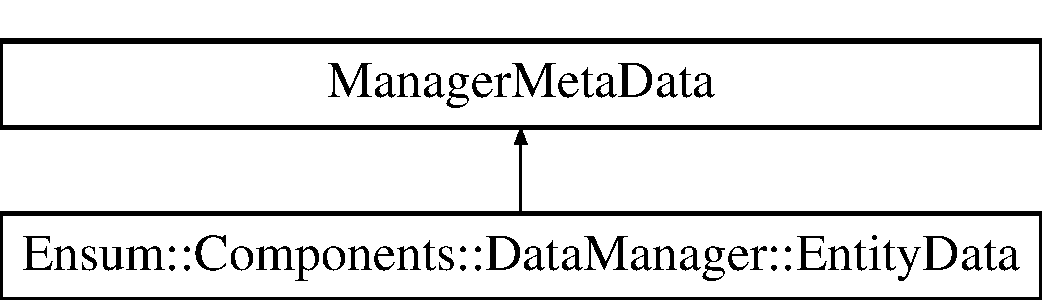
\includegraphics[height=2.000000cm]{struct_ensum_1_1_components_1_1_data_manager_1_1_entity_data}
\end{center}
\end{figure}
\subsection*{Public Attributes}
\begin{DoxyCompactItemize}
\item 
\hyperlink{struct_ensum_1_1_components_1_1_data_manager_1_1_data_buffer}{Data\+Buffer} $\ast$$\ast$ {\bfseries data\+Buff}\hypertarget{struct_ensum_1_1_components_1_1_data_manager_1_1_entity_data_aaab508d0e5ef00b27e1ec6f58b397657}{}\label{struct_ensum_1_1_components_1_1_data_manager_1_1_entity_data_aaab508d0e5ef00b27e1ec6f58b397657}

\end{DoxyCompactItemize}


\subsection{Detailed Description}
The managers data struct. 

The documentation for this struct was generated from the following file\+:\begin{DoxyCompactItemize}
\item 
Includes/\+Ensum\+\_\+components/Data\+Manager.\+h\end{DoxyCompactItemize}

\hypertarget{struct_ensum_1_1_components_1_1_entity_hasher}{}\section{Ensum\+:\+:Components\+:\+:Entity\+Hasher Struct Reference}
\label{struct_ensum_1_1_components_1_1_entity_hasher}\index{Ensum\+::\+Components\+::\+Entity\+Hasher@{Ensum\+::\+Components\+::\+Entity\+Hasher}}


Hasher for hashmaps.  




{\ttfamily \#include $<$Entity.\+h$>$}

\subsection*{Public Member Functions}
\begin{DoxyCompactItemize}
\item 
std\+::size\+\_\+t {\bfseries operator()} (const \hyperlink{struct_ensum_1_1_components_1_1_entity}{Entity} \&key) const \hypertarget{struct_ensum_1_1_components_1_1_entity_hasher_a9d4b4eb8467c10ad0df24bb12f683c5b}{}\label{struct_ensum_1_1_components_1_1_entity_hasher_a9d4b4eb8467c10ad0df24bb12f683c5b}

\end{DoxyCompactItemize}


\subsection{Detailed Description}
Hasher for hashmaps. 

The documentation for this struct was generated from the following file\+:\begin{DoxyCompactItemize}
\item 
C\+:/\+Users/peter/\+Source/\+Repos/\+E\+N\+S\+U\+M/\+Ensum/\+Includes/\+Ensum\+\_\+components/Entity.\+h\end{DoxyCompactItemize}

\hypertarget{class_ensum_1_1_components_1_1_entity_manager}{}\section{Ensum\+:\+:Components\+:\+:Entity\+Manager Class Reference}
\label{class_ensum_1_1_components_1_1_entity_manager}\index{Ensum\+::\+Components\+::\+Entity\+Manager@{Ensum\+::\+Components\+::\+Entity\+Manager}}


Manages all entities in all scenes.  




{\ttfamily \#include $<$Entity\+Manager.\+h$>$}

\subsection*{Public Member Functions}
\begin{DoxyCompactItemize}
\item 
\hyperlink{struct_ensum_1_1_components_1_1_entity}{Entity} \hyperlink{class_ensum_1_1_components_1_1_entity_manager_a15c2795c73d625bcc2399bf59cea64b5}{Create} ()\hypertarget{class_ensum_1_1_components_1_1_entity_manager_a15c2795c73d625bcc2399bf59cea64b5}{}\label{class_ensum_1_1_components_1_1_entity_manager_a15c2795c73d625bcc2399bf59cea64b5}

\begin{DoxyCompactList}\small\item\em Creates an entity, and returns it. \end{DoxyCompactList}\item 
const void \hyperlink{class_ensum_1_1_components_1_1_entity_manager_a87651038fca34e5dac4641c3d257c486}{Add\+Delete\+Callback} (const \hyperlink{struct_ensum_1_1_components_1_1_entity}{Entity} \&entity, \hyperlink{class_ensum_1_1_delegate}{Delegate}$<$ const void(const \hyperlink{struct_ensum_1_1_components_1_1_entity}{Entity} \&entity)$>$ \&callback)\hypertarget{class_ensum_1_1_components_1_1_entity_manager_a87651038fca34e5dac4641c3d257c486}{}\label{class_ensum_1_1_components_1_1_entity_manager_a87651038fca34e5dac4641c3d257c486}

\begin{DoxyCompactList}\small\item\em Add the callback for the entity. \end{DoxyCompactList}\item 
const bool \hyperlink{class_ensum_1_1_components_1_1_entity_manager_aa30d3768a9f92b138a52b7ac7c6045cc}{Alive} (const \hyperlink{struct_ensum_1_1_components_1_1_entity}{Entity} \&entity) const \hypertarget{class_ensum_1_1_components_1_1_entity_manager_aa30d3768a9f92b138a52b7ac7c6045cc}{}\label{class_ensum_1_1_components_1_1_entity_manager_aa30d3768a9f92b138a52b7ac7c6045cc}

\begin{DoxyCompactList}\small\item\em Determines whether or not the entity is alive. \end{DoxyCompactList}\item 
const void \hyperlink{class_ensum_1_1_components_1_1_entity_manager_aaa8e8f7e613b8b8d8b707dd80a43aec5}{Delete} (const \hyperlink{struct_ensum_1_1_components_1_1_entity}{Entity} \&entity)\hypertarget{class_ensum_1_1_components_1_1_entity_manager_aaa8e8f7e613b8b8d8b707dd80a43aec5}{}\label{class_ensum_1_1_components_1_1_entity_manager_aaa8e8f7e613b8b8d8b707dd80a43aec5}

\begin{DoxyCompactList}\small\item\em Deletes an alive entity. \end{DoxyCompactList}\end{DoxyCompactItemize}
\subsection*{Private Attributes}
\begin{DoxyCompactItemize}
\item 
std\+::vector$<$ uint8\+\_\+t $>$ $\ast$ {\bfseries \+\_\+generation}\hypertarget{class_ensum_1_1_components_1_1_entity_manager_a4eb470bc60cab8633f8a9811cb9a139f}{}\label{class_ensum_1_1_components_1_1_entity_manager_a4eb470bc60cab8633f8a9811cb9a139f}

\item 
std\+::deque$<$ uint32\+\_\+t $>$ $\ast$ {\bfseries \+\_\+free\+Indices}\hypertarget{class_ensum_1_1_components_1_1_entity_manager_aa90213c24c2e4f8f8c09f9cf1c21a613}{}\label{class_ensum_1_1_components_1_1_entity_manager_aa90213c24c2e4f8f8c09f9cf1c21a613}

\item 
std\+::vector$<$ \hyperlink{class_ensum_1_1_event}{Event}$<$ const void(const \hyperlink{struct_ensum_1_1_components_1_1_entity}{Entity} \&entity)$>$ $>$ $\ast$ {\bfseries \+\_\+destroy\+Callback}\hypertarget{class_ensum_1_1_components_1_1_entity_manager_a1f9c14dc1c320228130200a49fa08b9b}{}\label{class_ensum_1_1_components_1_1_entity_manager_a1f9c14dc1c320228130200a49fa08b9b}

\end{DoxyCompactItemize}
\subsection*{Static Private Attributes}
\begin{DoxyCompactItemize}
\item 
static const uint16\+\_\+t {\bfseries M\+I\+N\+I\+M\+U\+M\+\_\+\+F\+R\+E\+E\+\_\+\+I\+N\+D\+I\+C\+ES} = 1024U\hypertarget{class_ensum_1_1_components_1_1_entity_manager_a6d7bbd2c0c226a051f49382015c24962}{}\label{class_ensum_1_1_components_1_1_entity_manager_a6d7bbd2c0c226a051f49382015c24962}

\end{DoxyCompactItemize}


\subsection{Detailed Description}
Manages all entities in all scenes. 

The documentation for this class was generated from the following file\+:\begin{DoxyCompactItemize}
\item 
C\+:/\+Users/peter/\+Source/\+Repos/\+E\+N\+S\+U\+M/\+Ensum/\+Includes/\+Ensum\+\_\+components/Entity\+Manager.\+h\end{DoxyCompactItemize}

\hypertarget{struct_ensum_1_1_components_1_1_data_manager_1_1_entry_header}{}\section{Ensum\+:\+:Components\+:\+:Data\+Manager\+:\+:Entry\+Header Struct Reference}
\label{struct_ensum_1_1_components_1_1_data_manager_1_1_entry_header}\index{Ensum\+::\+Components\+::\+Data\+Manager\+::\+Entry\+Header@{Ensum\+::\+Components\+::\+Data\+Manager\+::\+Entry\+Header}}


The header struct, used for keeping track of the data entries a entity has.  


\subsection*{Public Attributes}
\begin{DoxyCompactItemize}
\item 
uint8\+\_\+t {\bfseries capacity} = 0\hypertarget{struct_ensum_1_1_components_1_1_data_manager_1_1_entry_header_a654a83e048907493d3547112ce0caf6a}{}\label{struct_ensum_1_1_components_1_1_data_manager_1_1_entry_header_a654a83e048907493d3547112ce0caf6a}

\item 
uint8\+\_\+t {\bfseries entry\+Count} = 0\hypertarget{struct_ensum_1_1_components_1_1_data_manager_1_1_entry_header_aad8d696cdacd86dd94f72f8ddd906090}{}\label{struct_ensum_1_1_components_1_1_data_manager_1_1_entry_header_aad8d696cdacd86dd94f72f8ddd906090}

\item 
uint8\+\_\+t {\bfseries entry\+Size} = sizeof(uint32\+\_\+t) + sizeof(\hyperlink{class_ensum_1_1_components_1_1_data_manager_aad73f648c4aee3f0530463eb787a7d7c}{Data\+Type}) + sizeof(\hyperlink{struct_ensum_1_1_components_1_1_data_manager_1_1_value}{Value})\hypertarget{struct_ensum_1_1_components_1_1_data_manager_1_1_entry_header_ad853eb6deff5a8991708b4de7e002e3e}{}\label{struct_ensum_1_1_components_1_1_data_manager_1_1_entry_header_ad853eb6deff5a8991708b4de7e002e3e}

\item 
uint32\+\_\+t $\ast$ {\bfseries keys}\hypertarget{struct_ensum_1_1_components_1_1_data_manager_1_1_entry_header_a925affe1ceff27a218fc851a73c5a0dc}{}\label{struct_ensum_1_1_components_1_1_data_manager_1_1_entry_header_a925affe1ceff27a218fc851a73c5a0dc}

\item 
\hyperlink{class_ensum_1_1_components_1_1_data_manager_aad73f648c4aee3f0530463eb787a7d7c}{Data\+Type} $\ast$ {\bfseries type}\hypertarget{struct_ensum_1_1_components_1_1_data_manager_1_1_entry_header_ae0b45453ca2df2abc12c0600448a4de5}{}\label{struct_ensum_1_1_components_1_1_data_manager_1_1_entry_header_ae0b45453ca2df2abc12c0600448a4de5}

\item 
\hyperlink{struct_ensum_1_1_components_1_1_data_manager_1_1_value}{Value} $\ast$ {\bfseries value}\hypertarget{struct_ensum_1_1_components_1_1_data_manager_1_1_entry_header_a92f14dfc77b6ca30285d37fa95d1fb5d}{}\label{struct_ensum_1_1_components_1_1_data_manager_1_1_entry_header_a92f14dfc77b6ca30285d37fa95d1fb5d}

\end{DoxyCompactItemize}


\subsection{Detailed Description}
The header struct, used for keeping track of the data entries a entity has. 

The documentation for this struct was generated from the following file\+:\begin{DoxyCompactItemize}
\item 
C\+:/\+Users/peter/\+Source/\+Repos/\+E\+N\+S\+U\+M/\+Ensum/\+Includes/\+Ensum\+\_\+components/Data\+Manager.\+h\end{DoxyCompactItemize}

\hypertarget{class_ensum_1_1_event}{}\section{Ensum\+:\+:Event$<$ T $>$ Class Template Reference}
\label{class_ensum_1_1_event}\index{Ensum\+::\+Event$<$ T $>$@{Ensum\+::\+Event$<$ T $>$}}


What is this file? A delegate class that can be used to pass free functions or member functions to an event.  




{\ttfamily \#include $<$Event.\+h$>$}



\subsection{Detailed Description}
\subsubsection*{template$<$typename T$>$\\*
class Ensum\+::\+Event$<$ T $>$}

What is this file? A delegate class that can be used to pass free functions or member functions to an event. 

See more at \href{http://www.codeproject.com/Articles/11015/The-Impossibly-Fast-C-Delegates}{\tt http\+://www.\+codeproject.\+com/\+Articles/11015/\+The-\/\+Impossibly-\/\+Fast-\/\+C-\/\+Delegates} There doesn\textquotesingle{}t seem to exist a much simpler way. std\+::function was considered, but due to lack of an equality operator they cannot be compared, ergo they also cannot be unsubscribed. Game Coding Complete says that C\#-\/style events would be nice, but C++ doesn\textquotesingle{}t support them out of the box. They do note however that it can be done using alot of template magic, with emphasis on alot. This solution works, but the syntax is horrible.

The event itself is just a collection of delegates that should be called when the event occurs. Triggering the event is done by the one owning the event. 

The documentation for this class was generated from the following file\+:\begin{DoxyCompactItemize}
\item 
C\+:/\+Users/peter/\+Source/\+Repos/\+E\+N\+S\+U\+M/\+Ensum/\+Includes/Event.\+h\end{DoxyCompactItemize}

\hypertarget{class_ensum_1_1_event_3_01_return_type_07_arguments_8_8_8_08_4}{}\section{Ensum\+:\+:Event$<$ Return\+Type(Arguments...)$>$ Class Template Reference}
\label{class_ensum_1_1_event_3_01_return_type_07_arguments_8_8_8_08_4}\index{Ensum\+::\+Event$<$ Return\+Type(\+Arguments...)$>$@{Ensum\+::\+Event$<$ Return\+Type(\+Arguments...)$>$}}


What is this file? A delegate class that can be used to pass free functions or member functions to an event.  




{\ttfamily \#include $<$Event.\+h$>$}

\subsection*{Public Member Functions}
\begin{DoxyCompactItemize}
\item 
void {\bfseries operator()} (Arguments...\+params)\hypertarget{class_ensum_1_1_event_3_01_return_type_07_arguments_8_8_8_08_4_add7c448f8cc9a82ee4f3a533f549f092}{}\label{class_ensum_1_1_event_3_01_return_type_07_arguments_8_8_8_08_4_add7c448f8cc9a82ee4f3a533f549f092}

\item 
void {\bfseries operator+=} (const \hyperlink{class_ensum_1_1_delegate}{Delegate}$<$ Return\+Type(Arguments...)$>$ \&func)\hypertarget{class_ensum_1_1_event_3_01_return_type_07_arguments_8_8_8_08_4_a9d0c7cffb5c1b1340f312a88fd3f06ce}{}\label{class_ensum_1_1_event_3_01_return_type_07_arguments_8_8_8_08_4_a9d0c7cffb5c1b1340f312a88fd3f06ce}

\item 
void {\bfseries operator-\/=} (const \hyperlink{class_ensum_1_1_delegate}{Delegate}$<$ Return\+Type(Arguments...)$>$ \&func)\hypertarget{class_ensum_1_1_event_3_01_return_type_07_arguments_8_8_8_08_4_a17b8e30ebf66d670d9afc31568b64c01}{}\label{class_ensum_1_1_event_3_01_return_type_07_arguments_8_8_8_08_4_a17b8e30ebf66d670d9afc31568b64c01}

\item 
void {\bfseries Clear} ()\hypertarget{class_ensum_1_1_event_3_01_return_type_07_arguments_8_8_8_08_4_ac2079482906c55a1d66ec3c19502804d}{}\label{class_ensum_1_1_event_3_01_return_type_07_arguments_8_8_8_08_4_ac2079482906c55a1d66ec3c19502804d}

\end{DoxyCompactItemize}
\subsection*{Private Member Functions}
\begin{DoxyCompactItemize}
\item 
\hyperlink{class_ensum_1_1_event}{Event} \& {\bfseries operator=} (const \hyperlink{class_ensum_1_1_event}{Event} \&rhs)\hypertarget{class_ensum_1_1_event_3_01_return_type_07_arguments_8_8_8_08_4_ae4e35cd8a4fef4f6532cc4d25a852d01}{}\label{class_ensum_1_1_event_3_01_return_type_07_arguments_8_8_8_08_4_ae4e35cd8a4fef4f6532cc4d25a852d01}

\item 
{\bfseries Event} (const \hyperlink{class_ensum_1_1_event}{Event} \&other)\hypertarget{class_ensum_1_1_event_3_01_return_type_07_arguments_8_8_8_08_4_aa65f84516d6dda8f6a5036a0f0a114f3}{}\label{class_ensum_1_1_event_3_01_return_type_07_arguments_8_8_8_08_4_aa65f84516d6dda8f6a5036a0f0a114f3}

\end{DoxyCompactItemize}
\subsection*{Private Attributes}
\begin{DoxyCompactItemize}
\item 
std\+::list$<$ \hyperlink{class_ensum_1_1_delegate}{Delegate}$<$ Return\+Type(Arguments...)$>$ $>$ $\ast$ {\bfseries \+\_\+callbacks}\hypertarget{class_ensum_1_1_event_3_01_return_type_07_arguments_8_8_8_08_4_a9d2ecb32fbc73454985d470c673336a9}{}\label{class_ensum_1_1_event_3_01_return_type_07_arguments_8_8_8_08_4_a9d2ecb32fbc73454985d470c673336a9}

\end{DoxyCompactItemize}


\subsection{Detailed Description}
\subsubsection*{template$<$typename Return\+Type, typename... Arguments$>$\\*
class Ensum\+::\+Event$<$ Return\+Type(\+Arguments...)$>$}

What is this file? A delegate class that can be used to pass free functions or member functions to an event. 

See more at \href{http://www.codeproject.com/Articles/11015/The-Impossibly-Fast-C-Delegates}{\tt http\+://www.\+codeproject.\+com/\+Articles/11015/\+The-\/\+Impossibly-\/\+Fast-\/\+C-\/\+Delegates} There doesn\textquotesingle{}t seem to exist a much simpler way. std\+::function was considered, but due to lack of an equality operator they cannot be compared, ergo they also cannot be unsubscribed. Game Coding Complete says that C\#-\/style events would be nice, but C++ doesn\textquotesingle{}t support them out of the box. They do note however that it can be done using alot of template magic, with emphasis on alot. This solution works, but the syntax is horrible.

The event itself is just a collection of delegates that should be called when the event occurs. Triggering the event is done by the one owning the event. 

The documentation for this class was generated from the following file\+:\begin{DoxyCompactItemize}
\item 
C\+:/\+Users/peter/\+Source/\+Repos/\+E\+N\+S\+U\+M/\+Ensum/\+Includes/Event.\+h\end{DoxyCompactItemize}

\hypertarget{class_ensum_1_1_exce}{}\section{Ensum\+:\+:Exce Class Reference}
\label{class_ensum_1_1_exce}\index{Ensum\+::\+Exce@{Ensum\+::\+Exce}}


Class used when throwing exceptions.  




{\ttfamily \#include $<$Exception.\+h$>$}

\subsection*{Public Member Functions}
\begin{DoxyCompactItemize}
\item 
{\bfseries Exce} (const std\+::exception \&e)\hypertarget{class_ensum_1_1_exce_aac9da3566349e2b459a0180dd30dc678}{}\label{class_ensum_1_1_exce_aac9da3566349e2b459a0180dd30dc678}

\item 
{\bfseries Exce} (const char $\ast$msg,...)\hypertarget{class_ensum_1_1_exce_a041cfe2bc0b98817568d9defb37bd98a}{}\label{class_ensum_1_1_exce_a041cfe2bc0b98817568d9defb37bd98a}

\item 
const void \hyperlink{class_ensum_1_1_exce_a0ae40fb8875bbc48afeedac6ba8a8804}{Print} () const \hypertarget{class_ensum_1_1_exce_a0ae40fb8875bbc48afeedac6ba8a8804}{}\label{class_ensum_1_1_exce_a0ae40fb8875bbc48afeedac6ba8a8804}

\begin{DoxyCompactList}\small\item\em Displayes a promt window of the exception. \end{DoxyCompactList}\end{DoxyCompactItemize}
\subsection*{Private Attributes}
\begin{DoxyCompactItemize}
\item 
\hyperlink{class_ensum_1_1string}{string} {\bfseries \+\_\+msg}\hypertarget{class_ensum_1_1_exce_accefd5af2666c691ad2b4a682ff59057}{}\label{class_ensum_1_1_exce_accefd5af2666c691ad2b4a682ff59057}

\item 
\hyperlink{class_ensum_1_1string}{string} {\bfseries \+\_\+cap}\hypertarget{class_ensum_1_1_exce_a9af3c82ac2580a4f72d342e7d359dadd}{}\label{class_ensum_1_1_exce_a9af3c82ac2580a4f72d342e7d359dadd}

\end{DoxyCompactItemize}


\subsection{Detailed Description}
Class used when throwing exceptions. 

The documentation for this class was generated from the following file\+:\begin{DoxyCompactItemize}
\item 
C\+:/\+Users/peter/\+Source/\+Repos/\+E\+N\+S\+U\+M/\+Ensum/\+Includes/Exception.\+h\end{DoxyCompactItemize}

\hypertarget{struct_ensum_1_1_file_handler_1_1_face}{}\section{Ensum\+:\+:File\+Handler\+:\+:Face Struct Reference}
\label{struct_ensum_1_1_file_handler_1_1_face}\index{Ensum\+::\+File\+Handler\+::\+Face@{Ensum\+::\+File\+Handler\+::\+Face}}
\subsection*{Public Member Functions}
\begin{DoxyCompactItemize}
\item 
{\bfseries Face} (vector$<$ vector$<$ uint64\+\_\+t $>$$>$ \&face)\hypertarget{struct_ensum_1_1_file_handler_1_1_face_ac35968c5cc028647f3a0ab65b87ca7ce}{}\label{struct_ensum_1_1_file_handler_1_1_face_ac35968c5cc028647f3a0ab65b87ca7ce}

\end{DoxyCompactItemize}
\subsection*{Public Attributes}
\begin{DoxyCompactItemize}
\item 
uint8\+\_\+t {\bfseries index\+Count}\hypertarget{struct_ensum_1_1_file_handler_1_1_face_a2f54ed62b9413df72a60011724ed1ce6}{}\label{struct_ensum_1_1_file_handler_1_1_face_a2f54ed62b9413df72a60011724ed1ce6}

\item 
\hyperlink{struct_ensum_1_1_file_handler_1_1_indices}{Indices} {\bfseries indices} \mbox{[}4\mbox{]}\hypertarget{struct_ensum_1_1_file_handler_1_1_face_a50b3ad717679c1ff96f06192a191a48a}{}\label{struct_ensum_1_1_file_handler_1_1_face_a50b3ad717679c1ff96f06192a191a48a}

\end{DoxyCompactItemize}


The documentation for this struct was generated from the following file\+:\begin{DoxyCompactItemize}
\item 
C\+:/\+Users/peter/\+Source/\+Repos/\+E\+N\+S\+U\+M/\+Ensum/\+Includes/\+Ensum\+\_\+filehandler/Mesh.\+h\end{DoxyCompactItemize}

\hypertarget{class_ensum_1_1_graphics_1_1_graphics}{}\section{Ensum\+:\+:Graphics\+:\+:Graphics Class Reference}
\label{class_ensum_1_1_graphics_1_1_graphics}\index{Ensum\+::\+Graphics\+::\+Graphics@{Ensum\+::\+Graphics\+::\+Graphics}}


The graphics interface.  




{\ttfamily \#include $<$Graphics.\+h$>$}

Inheritance diagram for Ensum\+:\+:Graphics\+:\+:Graphics\+:\begin{figure}[H]
\begin{center}
\leavevmode
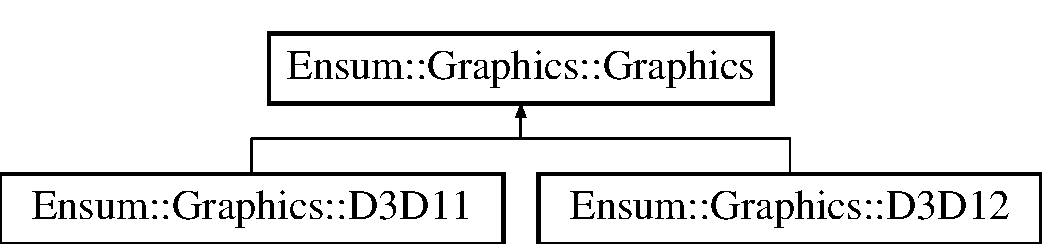
\includegraphics[height=2.000000cm]{class_ensum_1_1_graphics_1_1_graphics}
\end{center}
\end{figure}
\subsection*{Public Member Functions}
\begin{DoxyCompactItemize}
\item 
virtual const void \hyperlink{class_ensum_1_1_graphics_1_1_graphics_a79cd1971eb83f2b53707a1f71c764c9b}{Start} ()
\begin{DoxyCompactList}\small\item\em Enters the render loop. \end{DoxyCompactList}\item 
virtual const void \hyperlink{class_ensum_1_1_graphics_1_1_graphics_a22a9971757d8c9f56e4006ac50219995}{On\+Create\+Device} ()=0\hypertarget{class_ensum_1_1_graphics_1_1_graphics_a22a9971757d8c9f56e4006ac50219995}{}\label{class_ensum_1_1_graphics_1_1_graphics_a22a9971757d8c9f56e4006ac50219995}

\begin{DoxyCompactList}\small\item\em Implements the device creation. \end{DoxyCompactList}\item 
virtual const void \hyperlink{class_ensum_1_1_graphics_1_1_graphics_af26be2e7d907fc3ebaa587d12be9870c}{On\+Destroy\+Device} ()=0\hypertarget{class_ensum_1_1_graphics_1_1_graphics_af26be2e7d907fc3ebaa587d12be9870c}{}\label{class_ensum_1_1_graphics_1_1_graphics_af26be2e7d907fc3ebaa587d12be9870c}

\begin{DoxyCompactList}\small\item\em Implements the device destruction. \end{DoxyCompactList}\item 
virtual const \hyperlink{class_ensum_1_1string}{string} \& \hyperlink{class_ensum_1_1_graphics_1_1_graphics_ab336b7193886a85365b831eb34ecdc96}{Get\+Graphics\+Type} ()\hypertarget{class_ensum_1_1_graphics_1_1_graphics_ab336b7193886a85365b831eb34ecdc96}{}\label{class_ensum_1_1_graphics_1_1_graphics_ab336b7193886a85365b831eb34ecdc96}

\begin{DoxyCompactList}\small\item\em Returns what graphics type the current instance is. \end{DoxyCompactList}\item 
virtual const void \hyperlink{class_ensum_1_1_graphics_1_1_graphics_af653ac5e04559d540521f297c1b45109}{Start\+Thread} ()\hypertarget{class_ensum_1_1_graphics_1_1_graphics_af653ac5e04559d540521f297c1b45109}{}\label{class_ensum_1_1_graphics_1_1_graphics_af653ac5e04559d540521f297c1b45109}

\begin{DoxyCompactList}\small\item\em Creates the thread and executes it. \end{DoxyCompactList}\item 
virtual const void \hyperlink{class_ensum_1_1_graphics_1_1_graphics_a42ab0b6aa0d00eb926de5afef3ce1f9c}{Stop\+Thread} ()\hypertarget{class_ensum_1_1_graphics_1_1_graphics_a42ab0b6aa0d00eb926de5afef3ce1f9c}{}\label{class_ensum_1_1_graphics_1_1_graphics_a42ab0b6aa0d00eb926de5afef3ce1f9c}

\begin{DoxyCompactList}\small\item\em Stops the thread. \end{DoxyCompactList}\end{DoxyCompactItemize}
\subsection*{Static Public Member Functions}
\begin{DoxyCompactItemize}
\item 
static const void \hyperlink{class_ensum_1_1_graphics_1_1_graphics_a752ebdfc026c69ecc90f565e196ce726}{Create\+Instance} (\hyperlink{class_ensum_1_1_graphics_1_1_graphics}{Graphics} $\ast$g)
\begin{DoxyCompactList}\small\item\em Takes the pointer and initializes the graphics. \end{DoxyCompactList}\item 
static const void \hyperlink{class_ensum_1_1_graphics_1_1_graphics_a266c9b4cab940ccc392889be05d17d17}{Delete\+Instance} ()\hypertarget{class_ensum_1_1_graphics_1_1_graphics_a266c9b4cab940ccc392889be05d17d17}{}\label{class_ensum_1_1_graphics_1_1_graphics_a266c9b4cab940ccc392889be05d17d17}

\begin{DoxyCompactList}\small\item\em Deletes the graphics instance. \end{DoxyCompactList}\item 
static \hyperlink{struct_ensum_1_1_file_handler_1_1_mesh_data}{File\+Handler\+::\+Mesh\+Data} \hyperlink{class_ensum_1_1_graphics_1_1_graphics_acea2ccecffb6f21bd9d5ddb250879e07}{Create\+Mesh\+Data} (\hyperlink{class_ensum_1_1_file_handler_1_1_mesh}{File\+Handler\+::\+Mesh} \&mesh)\hypertarget{class_ensum_1_1_graphics_1_1_graphics_acea2ccecffb6f21bd9d5ddb250879e07}{}\label{class_ensum_1_1_graphics_1_1_graphics_acea2ccecffb6f21bd9d5ddb250879e07}

\begin{DoxyCompactList}\small\item\em Interleaves the meshdata and orders the creation of buffers for the mesh. \end{DoxyCompactList}\end{DoxyCompactItemize}
\subsection*{Protected Member Functions}
\begin{DoxyCompactItemize}
\item 
{\bfseries Graphics} (const \hyperlink{class_ensum_1_1string}{string} \&type)\hypertarget{class_ensum_1_1_graphics_1_1_graphics_ad8b5c80d5999b74320aa9bf13dead117}{}\label{class_ensum_1_1_graphics_1_1_graphics_ad8b5c80d5999b74320aa9bf13dead117}

\item 
virtual const void \hyperlink{class_ensum_1_1_graphics_1_1_graphics_a530a469dbfc96e4224c916f2253b8764}{\+\_\+\+On\+Options\+Change} ()=0
\begin{DoxyCompactList}\small\item\em Loads a mesh and creates a vertex and indexbuffer ID of mesh is returned. \end{DoxyCompactList}\item 
virtual const void \hyperlink{class_ensum_1_1_graphics_1_1_graphics_a79847436ca7588f8e3af99342461206c}{\+\_\+\+Begin\+Frame} (void)=0\hypertarget{class_ensum_1_1_graphics_1_1_graphics_a79847436ca7588f8e3af99342461206c}{}\label{class_ensum_1_1_graphics_1_1_graphics_a79847436ca7588f8e3af99342461206c}

\begin{DoxyCompactList}\small\item\em Begin the rendering frame. \end{DoxyCompactList}\item 
virtual const void \hyperlink{class_ensum_1_1_graphics_1_1_graphics_a0bdc9c86d0b314d6243e25c22eaecff9}{\+\_\+\+End\+Frame} (void)=0\hypertarget{class_ensum_1_1_graphics_1_1_graphics_a0bdc9c86d0b314d6243e25c22eaecff9}{}\label{class_ensum_1_1_graphics_1_1_graphics_a0bdc9c86d0b314d6243e25c22eaecff9}

\begin{DoxyCompactList}\small\item\em End the rendering frame. \end{DoxyCompactList}\item 
virtual const void \hyperlink{class_ensum_1_1_graphics_1_1_graphics_a0bf982fe118c7cbb23ad900509222e35}{\+\_\+\+Frame} ()=0\hypertarget{class_ensum_1_1_graphics_1_1_graphics_a0bf982fe118c7cbb23ad900509222e35}{}\label{class_ensum_1_1_graphics_1_1_graphics_a0bf982fe118c7cbb23ad900509222e35}

\begin{DoxyCompactList}\small\item\em What happens between Begin\+Frame and End\+Frame. \end{DoxyCompactList}\end{DoxyCompactItemize}
\subsection*{Protected Attributes}
\begin{DoxyCompactItemize}
\item 
H\+A\+N\+D\+LE {\bfseries \+\_\+options\+Change\+Mutex}\hypertarget{class_ensum_1_1_graphics_1_1_graphics_a486430a6a88ac0c0d6b96cefcab105c3}{}\label{class_ensum_1_1_graphics_1_1_graphics_a486430a6a88ac0c0d6b96cefcab105c3}

\item 
H\+A\+N\+D\+LE {\bfseries \+\_\+thread\+Handle}\hypertarget{class_ensum_1_1_graphics_1_1_graphics_aa876c80ddab2979f0f981579fcad4a5e}{}\label{class_ensum_1_1_graphics_1_1_graphics_aa876c80ddab2979f0f981579fcad4a5e}

\item 
D\+W\+O\+RD {\bfseries \+\_\+thread\+Address}\hypertarget{class_ensum_1_1_graphics_1_1_graphics_a35a7545f0e91b48c4fc356d47cb902e4}{}\label{class_ensum_1_1_graphics_1_1_graphics_a35a7545f0e91b48c4fc356d47cb902e4}

\item 
bool {\bfseries \+\_\+shutdown}\hypertarget{class_ensum_1_1_graphics_1_1_graphics_aeb14afd8bd18405619070141bee75db6}{}\label{class_ensum_1_1_graphics_1_1_graphics_aeb14afd8bd18405619070141bee75db6}

\item 
bool {\bfseries \+\_\+fullscreen}\hypertarget{class_ensum_1_1_graphics_1_1_graphics_af9417ebb67c1d375ca922bb4dcb0d761}{}\label{class_ensum_1_1_graphics_1_1_graphics_af9417ebb67c1d375ca922bb4dcb0d761}

\item 
unsigned {\bfseries \+\_\+width}\hypertarget{class_ensum_1_1_graphics_1_1_graphics_aca92665104053a5d47daa843e89cace6}{}\label{class_ensum_1_1_graphics_1_1_graphics_aca92665104053a5d47daa843e89cace6}

\item 
unsigned {\bfseries \+\_\+height}\hypertarget{class_ensum_1_1_graphics_1_1_graphics_a062bb53f418490d51cddb757421dccf1}{}\label{class_ensum_1_1_graphics_1_1_graphics_a062bb53f418490d51cddb757421dccf1}

\item 
bool {\bfseries \+\_\+vsync}\hypertarget{class_ensum_1_1_graphics_1_1_graphics_ab72c0acc92e99f35b05f3f18be3a4ca8}{}\label{class_ensum_1_1_graphics_1_1_graphics_ab72c0acc92e99f35b05f3f18be3a4ca8}

\item 
\hyperlink{class_ensum_1_1string}{string} {\bfseries \+\_\+type}\hypertarget{class_ensum_1_1_graphics_1_1_graphics_a1712f52c5d4a3d9af81f9a0b53806d84}{}\label{class_ensum_1_1_graphics_1_1_graphics_a1712f52c5d4a3d9af81f9a0b53806d84}

\end{DoxyCompactItemize}
\subsection*{Static Protected Attributes}
\begin{DoxyCompactItemize}
\item 
static \hyperlink{class_ensum_1_1_graphics_1_1_graphics}{Graphics} $\ast$ {\bfseries \+\_\+instance}\hypertarget{class_ensum_1_1_graphics_1_1_graphics_a42490e399a8dbe1b5516033938522b84}{}\label{class_ensum_1_1_graphics_1_1_graphics_a42490e399a8dbe1b5516033938522b84}

\end{DoxyCompactItemize}


\subsection{Detailed Description}
The graphics interface. 

When an instance of the graphics is created it will connect with a sceneprovider which in turn provides the graphics with render jobs. The graphics is runs on its own thread and will only interact with the rest when gathering jobs. 

\subsection{Member Function Documentation}
\index{Ensum\+::\+Graphics\+::\+Graphics@{Ensum\+::\+Graphics\+::\+Graphics}!\+\_\+\+On\+Options\+Change@{\+\_\+\+On\+Options\+Change}}
\index{\+\_\+\+On\+Options\+Change@{\+\_\+\+On\+Options\+Change}!Ensum\+::\+Graphics\+::\+Graphics@{Ensum\+::\+Graphics\+::\+Graphics}}
\subsubsection[{\texorpdfstring{\+\_\+\+On\+Options\+Change()=0}{_OnOptionsChange()=0}}]{\setlength{\rightskip}{0pt plus 5cm}virtual const void Ensum\+::\+Graphics\+::\+Graphics\+::\+\_\+\+On\+Options\+Change (
\begin{DoxyParamCaption}
{}
\end{DoxyParamCaption}
)\hspace{0.3cm}{\ttfamily [protected]}, {\ttfamily [pure virtual]}}\hypertarget{class_ensum_1_1_graphics_1_1_graphics_a530a469dbfc96e4224c916f2253b8764}{}\label{class_ensum_1_1_graphics_1_1_graphics_a530a469dbfc96e4224c916f2253b8764}


Loads a mesh and creates a vertex and indexbuffer ID of mesh is returned. 

Use flag to indicate loading and unloading for mesh.\+Called when the options have changed. 

Implemented in \hyperlink{class_ensum_1_1_graphics_1_1_d3_d12_ad276cdc2f03df54cbbb7d05ac8785df4}{Ensum\+::\+Graphics\+::\+D3\+D12}, and \hyperlink{class_ensum_1_1_graphics_1_1_d3_d11_aaa1f9118226ed14729d1d1ad450ec10d}{Ensum\+::\+Graphics\+::\+D3\+D11}.

\index{Ensum\+::\+Graphics\+::\+Graphics@{Ensum\+::\+Graphics\+::\+Graphics}!Create\+Instance@{Create\+Instance}}
\index{Create\+Instance@{Create\+Instance}!Ensum\+::\+Graphics\+::\+Graphics@{Ensum\+::\+Graphics\+::\+Graphics}}
\subsubsection[{\texorpdfstring{Create\+Instance(\+Graphics $\ast$g)}{CreateInstance(Graphics *g)}}]{\setlength{\rightskip}{0pt plus 5cm}static const void Ensum\+::\+Graphics\+::\+Graphics\+::\+Create\+Instance (
\begin{DoxyParamCaption}
\item[{{\bf Graphics} $\ast$}]{g}
\end{DoxyParamCaption}
)\hspace{0.3cm}{\ttfamily [static]}}\hypertarget{class_ensum_1_1_graphics_1_1_graphics_a752ebdfc026c69ecc90f565e196ce726}{}\label{class_ensum_1_1_graphics_1_1_graphics_a752ebdfc026c69ecc90f565e196ce726}


Takes the pointer and initializes the graphics. 

This function calls the On\+Create\+Device then the Start\+Thread function. \index{Ensum\+::\+Graphics\+::\+Graphics@{Ensum\+::\+Graphics\+::\+Graphics}!Start@{Start}}
\index{Start@{Start}!Ensum\+::\+Graphics\+::\+Graphics@{Ensum\+::\+Graphics\+::\+Graphics}}
\subsubsection[{\texorpdfstring{Start()}{Start()}}]{\setlength{\rightskip}{0pt plus 5cm}virtual const void Ensum\+::\+Graphics\+::\+Graphics\+::\+Start (
\begin{DoxyParamCaption}
{}
\end{DoxyParamCaption}
)\hspace{0.3cm}{\ttfamily [virtual]}}\hypertarget{class_ensum_1_1_graphics_1_1_graphics_a79cd1971eb83f2b53707a1f71c764c9b}{}\label{class_ensum_1_1_graphics_1_1_graphics_a79cd1971eb83f2b53707a1f71c764c9b}


Enters the render loop. 

This should only be called inside the thread. 

The documentation for this class was generated from the following file\+:\begin{DoxyCompactItemize}
\item 
C\+:/\+Users/peter/\+Source/\+Repos/\+E\+N\+S\+U\+M/\+Ensum/\+Includes/\+Ensum\+\_\+graphics/Graphics.\+h\end{DoxyCompactItemize}

\hypertarget{struct_ensum_1_1_graphics_1_1_direct3_d12_1_1_index_buffer}{}\section{Ensum\+:\+:Graphics\+:\+:Direct3\+D12\+:\+:Index\+Buffer Struct Reference}
\label{struct_ensum_1_1_graphics_1_1_direct3_d12_1_1_index_buffer}\index{Ensum\+::\+Graphics\+::\+Direct3\+D12\+::\+Index\+Buffer@{Ensum\+::\+Graphics\+::\+Direct3\+D12\+::\+Index\+Buffer}}
\subsection*{Public Attributes}
\begin{DoxyCompactItemize}
\item 
Com\+Ptr$<$ I\+D3\+D12\+Resource $>$ {\bfseries buffer}\hypertarget{struct_ensum_1_1_graphics_1_1_direct3_d12_1_1_index_buffer_a139d2959ce47f53d17ab0bad080869a8}{}\label{struct_ensum_1_1_graphics_1_1_direct3_d12_1_1_index_buffer_a139d2959ce47f53d17ab0bad080869a8}

\item 
D3\+D12\+\_\+\+I\+N\+D\+E\+X\+\_\+\+B\+U\+F\+F\+E\+R\+\_\+\+V\+I\+EW {\bfseries view}\hypertarget{struct_ensum_1_1_graphics_1_1_direct3_d12_1_1_index_buffer_a87dacc5eeee5257e978c0b49fde4b514}{}\label{struct_ensum_1_1_graphics_1_1_direct3_d12_1_1_index_buffer_a87dacc5eeee5257e978c0b49fde4b514}

\end{DoxyCompactItemize}


The documentation for this struct was generated from the following file\+:\begin{DoxyCompactItemize}
\item 
C\+:/\+Users/peter/\+Source/\+Repos/\+E\+N\+S\+U\+M/\+Ensum/\+Includes/\+Ensum\+\_\+graphics/Direct3\+D12.\+h\end{DoxyCompactItemize}

\hypertarget{struct_ensum_1_1_file_handler_1_1_indices}{}\section{Ensum\+:\+:File\+Handler\+:\+:Indices Struct Reference}
\label{struct_ensum_1_1_file_handler_1_1_indices}\index{Ensum\+::\+File\+Handler\+::\+Indices@{Ensum\+::\+File\+Handler\+::\+Indices}}
\subsection*{Public Attributes}
\begin{DoxyCompactItemize}
\item 
uint8\+\_\+t {\bfseries index\+Count}\hypertarget{struct_ensum_1_1_file_handler_1_1_indices_afe85a0ec09149ff55b89c06fe097486d}{}\label{struct_ensum_1_1_file_handler_1_1_indices_afe85a0ec09149ff55b89c06fe097486d}

\item 
uint64\+\_\+t {\bfseries index} \mbox{[}4\mbox{]}\hypertarget{struct_ensum_1_1_file_handler_1_1_indices_a912cc220a04acf4ba42c1fa576a41e44}{}\label{struct_ensum_1_1_file_handler_1_1_indices_a912cc220a04acf4ba42c1fa576a41e44}

\end{DoxyCompactItemize}


The documentation for this struct was generated from the following file\+:\begin{DoxyCompactItemize}
\item 
C\+:/\+Users/peter/\+Source/\+Repos/\+E\+N\+S\+U\+M/\+Ensum/\+Includes/\+Ensum\+\_\+filehandler/Mesh.\+h\end{DoxyCompactItemize}

\hypertarget{struct_ensum_1_1_graphics_1_1_indirect_args_buffer}{}\section{Ensum\+:\+:Graphics\+:\+:Indirect\+Args\+Buffer Struct Reference}
\label{struct_ensum_1_1_graphics_1_1_indirect_args_buffer}\index{Ensum\+::\+Graphics\+::\+Indirect\+Args\+Buffer@{Ensum\+::\+Graphics\+::\+Indirect\+Args\+Buffer}}
\subsection*{Public Attributes}
\begin{DoxyCompactItemize}
\item 
I\+D3\+D11\+Buffer $\ast$ {\bfseries Buffer} = nullptr\hypertarget{struct_ensum_1_1_graphics_1_1_indirect_args_buffer_a3538f8910f284103d53c74ab46a7e6c7}{}\label{struct_ensum_1_1_graphics_1_1_indirect_args_buffer_a3538f8910f284103d53c74ab46a7e6c7}

\item 
unsigned {\bfseries Size} = 0\hypertarget{struct_ensum_1_1_graphics_1_1_indirect_args_buffer_ae69b1b5c792347d5dae6b060109ff8b6}{}\label{struct_ensum_1_1_graphics_1_1_indirect_args_buffer_ae69b1b5c792347d5dae6b060109ff8b6}

\end{DoxyCompactItemize}


The documentation for this struct was generated from the following file\+:\begin{DoxyCompactItemize}
\item 
C\+:/\+Users/peter/\+Source/\+Repos/\+E\+N\+S\+U\+M/\+Ensum/\+Includes/\+Ensum\+\_\+graphics/Direct3\+D11.\+h\end{DoxyCompactItemize}

\hypertarget{class_ensum_1_1_file_handler_1_1ini}{}\section{Ensum\+:\+:File\+Handler\+:\+:ini Class Reference}
\label{class_ensum_1_1_file_handler_1_1ini}\index{Ensum\+::\+File\+Handler\+::ini@{Ensum\+::\+File\+Handler\+::ini}}


A wrapper class for ini files.  




{\ttfamily \#include $<$Ini.\+h$>$}

\subsection*{Classes}
\begin{DoxyCompactItemize}
\item 
struct \hyperlink{struct_ensum_1_1_file_handler_1_1ini_1_1_key}{Key}
\item 
struct \hyperlink{struct_ensum_1_1_file_handler_1_1ini_1_1_section}{Section}
\end{DoxyCompactItemize}
\subsection*{Public Member Functions}
\begin{DoxyCompactItemize}
\item 
{\bfseries ini} (const \hyperlink{class_ensum_1_1string}{string} \&path)\hypertarget{class_ensum_1_1_file_handler_1_1ini_a966aac9f2602195dd3f9c8353061c191}{}\label{class_ensum_1_1_file_handler_1_1ini_a966aac9f2602195dd3f9c8353061c191}

\item 
\hyperlink{class_ensum_1_1string}{string} \hyperlink{class_ensum_1_1_file_handler_1_1ini_a794d0729d8ac92954dc6adcfdc10888c}{Get} (const \hyperlink{class_ensum_1_1string}{string} \&section, const \hyperlink{class_ensum_1_1string}{string} \&name, const \hyperlink{class_ensum_1_1string}{string} \&default\+\_\+value) const 
\begin{DoxyCompactList}\small\item\em Looks up the value of the given name and section and returns it as a string. \end{DoxyCompactList}\item 
long \hyperlink{class_ensum_1_1_file_handler_1_1ini_a53a1834bf3a13d38c166e417ac1d2973}{Get\+Integer} (const \hyperlink{class_ensum_1_1string}{string} \&section, const \hyperlink{class_ensum_1_1string}{string} \&name, long default\+\_\+value) const 
\begin{DoxyCompactList}\small\item\em Looks up the value of the given name and section and returns it as a integer. \end{DoxyCompactList}\item 
double \hyperlink{class_ensum_1_1_file_handler_1_1ini_af0f24b8866a8c16c6b09d6f707a676b7}{Get\+Real} (const \hyperlink{class_ensum_1_1string}{string} \&section, const \hyperlink{class_ensum_1_1string}{string} \&name, double default\+\_\+value) const 
\begin{DoxyCompactList}\small\item\em Looks up the value of the given name and section and returns it as a real. \end{DoxyCompactList}\item 
bool \hyperlink{class_ensum_1_1_file_handler_1_1ini_a8a2d73e88459187df0c5b9d2880a08eb}{Get\+Boolean} (const \hyperlink{class_ensum_1_1string}{string} \&section, const \hyperlink{class_ensum_1_1string}{string} \&name, bool default\+\_\+value) const 
\begin{DoxyCompactList}\small\item\em Looks up the value of the given name and section and returns it as a boolean. \end{DoxyCompactList}\item 
const void \hyperlink{class_ensum_1_1_file_handler_1_1ini_a7981581cf337fa3829dc95bc3def5a72}{Set} (const \hyperlink{class_ensum_1_1string}{string} \&section, const \hyperlink{class_ensum_1_1string}{string} \&name, const \hyperlink{class_ensum_1_1string}{string} \&value)
\begin{DoxyCompactList}\small\item\em Set the string value of given name in given section. \end{DoxyCompactList}\item 
const void \hyperlink{class_ensum_1_1_file_handler_1_1ini_a1ed4f9fa3abb4a1ce94fafd64d348af6}{Set\+Integer} (const \hyperlink{class_ensum_1_1string}{string} \&section, const \hyperlink{class_ensum_1_1string}{string} \&name, long value)
\begin{DoxyCompactList}\small\item\em Set the integer value of given name in given section. \end{DoxyCompactList}\item 
const void \hyperlink{class_ensum_1_1_file_handler_1_1ini_ae628d6053f8e94a6acc8499961741317}{Set\+Real} (const \hyperlink{class_ensum_1_1string}{string} \&section, const \hyperlink{class_ensum_1_1string}{string} \&name, double value)
\begin{DoxyCompactList}\small\item\em Set the real value of given name in given section. \end{DoxyCompactList}\item 
const void \hyperlink{class_ensum_1_1_file_handler_1_1ini_ac31a3463aeec3b6c378e2b5a8f73de8f}{Set\+Boolean} (const \hyperlink{class_ensum_1_1string}{string} \&section, const \hyperlink{class_ensum_1_1string}{string} \&name, bool value)
\begin{DoxyCompactList}\small\item\em Set the boolean value of given name in given section. \end{DoxyCompactList}\end{DoxyCompactItemize}
\subsection*{Private Member Functions}
\begin{DoxyCompactItemize}
\item 
const void \hyperlink{class_ensum_1_1_file_handler_1_1ini_a413fd1029742025232f53d3020280245}{\+\_\+\+Parse\+Data} (std\+::ifstream \&file)
\begin{DoxyCompactList}\small\item\em Reads the ini file to buffer. \end{DoxyCompactList}\item 
const void \hyperlink{class_ensum_1_1_file_handler_1_1ini_ace94f563974a671c5249548934688c88}{\+\_\+\+Write\+Data} (std\+::ofstream \&file)\hypertarget{class_ensum_1_1_file_handler_1_1ini_ace94f563974a671c5249548934688c88}{}\label{class_ensum_1_1_file_handler_1_1ini_ace94f563974a671c5249548934688c88}

\begin{DoxyCompactList}\small\item\em Writes the buffer to file. \end{DoxyCompactList}\end{DoxyCompactItemize}
\subsection*{Private Attributes}
\begin{DoxyCompactItemize}
\item 
std\+::vector$<$ \hyperlink{struct_ensum_1_1_file_handler_1_1ini_1_1_section}{Section} $>$ $\ast$ {\bfseries \+\_\+sections}\hypertarget{class_ensum_1_1_file_handler_1_1ini_a3088b323acff5e13750fb5d9242b2f91}{}\label{class_ensum_1_1_file_handler_1_1ini_a3088b323acff5e13750fb5d9242b2f91}

\item 
\hyperlink{class_ensum_1_1string}{string} {\bfseries \+\_\+path}\hypertarget{class_ensum_1_1_file_handler_1_1ini_a3d544c876f6837be6ca027db706cbba6}{}\label{class_ensum_1_1_file_handler_1_1ini_a3d544c876f6837be6ca027db706cbba6}

\end{DoxyCompactItemize}


\subsection{Detailed Description}
A wrapper class for ini files. 

This class stores the values in given ini file and saves any new values on delete. 

\subsection{Member Function Documentation}
\index{Ensum\+::\+File\+Handler\+::ini@{Ensum\+::\+File\+Handler\+::ini}!\+\_\+\+Parse\+Data@{\+\_\+\+Parse\+Data}}
\index{\+\_\+\+Parse\+Data@{\+\_\+\+Parse\+Data}!Ensum\+::\+File\+Handler\+::ini@{Ensum\+::\+File\+Handler\+::ini}}
\subsubsection[{\texorpdfstring{\+\_\+\+Parse\+Data(std\+::ifstream \&file)}{_ParseData(std::ifstream &file)}}]{\setlength{\rightskip}{0pt plus 5cm}const void Ensum\+::\+File\+Handler\+::ini\+::\+\_\+\+Parse\+Data (
\begin{DoxyParamCaption}
\item[{std\+::ifstream \&}]{file}
\end{DoxyParamCaption}
)\hspace{0.3cm}{\ttfamily [private]}}\hypertarget{class_ensum_1_1_file_handler_1_1ini_a413fd1029742025232f53d3020280245}{}\label{class_ensum_1_1_file_handler_1_1ini_a413fd1029742025232f53d3020280245}


Reads the ini file to buffer. 

You can\textquotesingle{}t really call this parsing, but hey it works. \index{Ensum\+::\+File\+Handler\+::ini@{Ensum\+::\+File\+Handler\+::ini}!Get@{Get}}
\index{Get@{Get}!Ensum\+::\+File\+Handler\+::ini@{Ensum\+::\+File\+Handler\+::ini}}
\subsubsection[{\texorpdfstring{Get(const string \&section, const string \&name, const string \&default\+\_\+value) const }{Get(const string &section, const string &name, const string &default_value) const }}]{\setlength{\rightskip}{0pt plus 5cm}{\bf string} Ensum\+::\+File\+Handler\+::ini\+::\+Get (
\begin{DoxyParamCaption}
\item[{const {\bf string} \&}]{section, }
\item[{const {\bf string} \&}]{name, }
\item[{const {\bf string} \&}]{default\+\_\+value}
\end{DoxyParamCaption}
) const}\hypertarget{class_ensum_1_1_file_handler_1_1ini_a794d0729d8ac92954dc6adcfdc10888c}{}\label{class_ensum_1_1_file_handler_1_1ini_a794d0729d8ac92954dc6adcfdc10888c}


Looks up the value of the given name and section and returns it as a string. 

If the sectino/name was not found, the default\+\_\+value will be returned. \index{Ensum\+::\+File\+Handler\+::ini@{Ensum\+::\+File\+Handler\+::ini}!Get\+Boolean@{Get\+Boolean}}
\index{Get\+Boolean@{Get\+Boolean}!Ensum\+::\+File\+Handler\+::ini@{Ensum\+::\+File\+Handler\+::ini}}
\subsubsection[{\texorpdfstring{Get\+Boolean(const string \&section, const string \&name, bool default\+\_\+value) const }{GetBoolean(const string &section, const string &name, bool default_value) const }}]{\setlength{\rightskip}{0pt plus 5cm}bool Ensum\+::\+File\+Handler\+::ini\+::\+Get\+Boolean (
\begin{DoxyParamCaption}
\item[{const {\bf string} \&}]{section, }
\item[{const {\bf string} \&}]{name, }
\item[{bool}]{default\+\_\+value}
\end{DoxyParamCaption}
) const}\hypertarget{class_ensum_1_1_file_handler_1_1ini_a8a2d73e88459187df0c5b9d2880a08eb}{}\label{class_ensum_1_1_file_handler_1_1ini_a8a2d73e88459187df0c5b9d2880a08eb}


Looks up the value of the given name and section and returns it as a boolean. 

If the sectino/name was not found, the default\+\_\+value will be returned. \index{Ensum\+::\+File\+Handler\+::ini@{Ensum\+::\+File\+Handler\+::ini}!Get\+Integer@{Get\+Integer}}
\index{Get\+Integer@{Get\+Integer}!Ensum\+::\+File\+Handler\+::ini@{Ensum\+::\+File\+Handler\+::ini}}
\subsubsection[{\texorpdfstring{Get\+Integer(const string \&section, const string \&name, long default\+\_\+value) const }{GetInteger(const string &section, const string &name, long default_value) const }}]{\setlength{\rightskip}{0pt plus 5cm}long Ensum\+::\+File\+Handler\+::ini\+::\+Get\+Integer (
\begin{DoxyParamCaption}
\item[{const {\bf string} \&}]{section, }
\item[{const {\bf string} \&}]{name, }
\item[{long}]{default\+\_\+value}
\end{DoxyParamCaption}
) const}\hypertarget{class_ensum_1_1_file_handler_1_1ini_a53a1834bf3a13d38c166e417ac1d2973}{}\label{class_ensum_1_1_file_handler_1_1ini_a53a1834bf3a13d38c166e417ac1d2973}


Looks up the value of the given name and section and returns it as a integer. 

If the sectino/name was not found, the default\+\_\+value will be returned. \index{Ensum\+::\+File\+Handler\+::ini@{Ensum\+::\+File\+Handler\+::ini}!Get\+Real@{Get\+Real}}
\index{Get\+Real@{Get\+Real}!Ensum\+::\+File\+Handler\+::ini@{Ensum\+::\+File\+Handler\+::ini}}
\subsubsection[{\texorpdfstring{Get\+Real(const string \&section, const string \&name, double default\+\_\+value) const }{GetReal(const string &section, const string &name, double default_value) const }}]{\setlength{\rightskip}{0pt plus 5cm}double Ensum\+::\+File\+Handler\+::ini\+::\+Get\+Real (
\begin{DoxyParamCaption}
\item[{const {\bf string} \&}]{section, }
\item[{const {\bf string} \&}]{name, }
\item[{double}]{default\+\_\+value}
\end{DoxyParamCaption}
) const}\hypertarget{class_ensum_1_1_file_handler_1_1ini_af0f24b8866a8c16c6b09d6f707a676b7}{}\label{class_ensum_1_1_file_handler_1_1ini_af0f24b8866a8c16c6b09d6f707a676b7}


Looks up the value of the given name and section and returns it as a real. 

If the sectino/name was not found, the default\+\_\+value will be returned. \index{Ensum\+::\+File\+Handler\+::ini@{Ensum\+::\+File\+Handler\+::ini}!Set@{Set}}
\index{Set@{Set}!Ensum\+::\+File\+Handler\+::ini@{Ensum\+::\+File\+Handler\+::ini}}
\subsubsection[{\texorpdfstring{Set(const string \&section, const string \&name, const string \&value)}{Set(const string &section, const string &name, const string &value)}}]{\setlength{\rightskip}{0pt plus 5cm}const void Ensum\+::\+File\+Handler\+::ini\+::\+Set (
\begin{DoxyParamCaption}
\item[{const {\bf string} \&}]{section, }
\item[{const {\bf string} \&}]{name, }
\item[{const {\bf string} \&}]{value}
\end{DoxyParamCaption}
)}\hypertarget{class_ensum_1_1_file_handler_1_1ini_a7981581cf337fa3829dc95bc3def5a72}{}\label{class_ensum_1_1_file_handler_1_1ini_a7981581cf337fa3829dc95bc3def5a72}


Set the string value of given name in given section. 

If the sectino/name was not found they are added. \index{Ensum\+::\+File\+Handler\+::ini@{Ensum\+::\+File\+Handler\+::ini}!Set\+Boolean@{Set\+Boolean}}
\index{Set\+Boolean@{Set\+Boolean}!Ensum\+::\+File\+Handler\+::ini@{Ensum\+::\+File\+Handler\+::ini}}
\subsubsection[{\texorpdfstring{Set\+Boolean(const string \&section, const string \&name, bool value)}{SetBoolean(const string &section, const string &name, bool value)}}]{\setlength{\rightskip}{0pt plus 5cm}const void Ensum\+::\+File\+Handler\+::ini\+::\+Set\+Boolean (
\begin{DoxyParamCaption}
\item[{const {\bf string} \&}]{section, }
\item[{const {\bf string} \&}]{name, }
\item[{bool}]{value}
\end{DoxyParamCaption}
)}\hypertarget{class_ensum_1_1_file_handler_1_1ini_ac31a3463aeec3b6c378e2b5a8f73de8f}{}\label{class_ensum_1_1_file_handler_1_1ini_ac31a3463aeec3b6c378e2b5a8f73de8f}


Set the boolean value of given name in given section. 

If the sectino/name was not found they are added. \index{Ensum\+::\+File\+Handler\+::ini@{Ensum\+::\+File\+Handler\+::ini}!Set\+Integer@{Set\+Integer}}
\index{Set\+Integer@{Set\+Integer}!Ensum\+::\+File\+Handler\+::ini@{Ensum\+::\+File\+Handler\+::ini}}
\subsubsection[{\texorpdfstring{Set\+Integer(const string \&section, const string \&name, long value)}{SetInteger(const string &section, const string &name, long value)}}]{\setlength{\rightskip}{0pt plus 5cm}const void Ensum\+::\+File\+Handler\+::ini\+::\+Set\+Integer (
\begin{DoxyParamCaption}
\item[{const {\bf string} \&}]{section, }
\item[{const {\bf string} \&}]{name, }
\item[{long}]{value}
\end{DoxyParamCaption}
)}\hypertarget{class_ensum_1_1_file_handler_1_1ini_a1ed4f9fa3abb4a1ce94fafd64d348af6}{}\label{class_ensum_1_1_file_handler_1_1ini_a1ed4f9fa3abb4a1ce94fafd64d348af6}


Set the integer value of given name in given section. 

If the sectino/name was not found they are added. \index{Ensum\+::\+File\+Handler\+::ini@{Ensum\+::\+File\+Handler\+::ini}!Set\+Real@{Set\+Real}}
\index{Set\+Real@{Set\+Real}!Ensum\+::\+File\+Handler\+::ini@{Ensum\+::\+File\+Handler\+::ini}}
\subsubsection[{\texorpdfstring{Set\+Real(const string \&section, const string \&name, double value)}{SetReal(const string &section, const string &name, double value)}}]{\setlength{\rightskip}{0pt plus 5cm}const void Ensum\+::\+File\+Handler\+::ini\+::\+Set\+Real (
\begin{DoxyParamCaption}
\item[{const {\bf string} \&}]{section, }
\item[{const {\bf string} \&}]{name, }
\item[{double}]{value}
\end{DoxyParamCaption}
)}\hypertarget{class_ensum_1_1_file_handler_1_1ini_ae628d6053f8e94a6acc8499961741317}{}\label{class_ensum_1_1_file_handler_1_1ini_ae628d6053f8e94a6acc8499961741317}


Set the real value of given name in given section. 

If the sectino/name was not found they are added. 

The documentation for this class was generated from the following file\+:\begin{DoxyCompactItemize}
\item 
Includes/\+Ensum\+\_\+filehandler/Ini.\+h\end{DoxyCompactItemize}

\hypertarget{class_ensum_1_1_input_1_1_input}{}\section{Ensum\+:\+:Input\+:\+:Input Class Reference}
\label{class_ensum_1_1_input_1_1_input}\index{Ensum\+::\+Input\+::\+Input@{Ensum\+::\+Input\+::\+Input}}


Stores the states of the mouse and keyboard.  




{\ttfamily \#include $<$Input.\+h$>$}

\subsection*{Public Member Functions}
\begin{DoxyCompactItemize}
\item 
const void \hyperlink{class_ensum_1_1_input_1_1_input_aade076509ba0a3b50a5f60b0fbeedf3b}{Frame} ()
\begin{DoxyCompactList}\small\item\em Does frame updates. \end{DoxyCompactList}\item 
const bool \hyperlink{class_ensum_1_1_input_1_1_input_a5770ec02144e58c2cc56df1ff3c97815}{Is\+Key\+Down} (Keys key\+Code) const \hypertarget{class_ensum_1_1_input_1_1_input_a5770ec02144e58c2cc56df1ff3c97815}{}\label{class_ensum_1_1_input_1_1_input_a5770ec02144e58c2cc56df1ff3c97815}

\begin{DoxyCompactList}\small\item\em Returns whether specified key is down. \end{DoxyCompactList}\item 
const bool \hyperlink{class_ensum_1_1_input_1_1_input_a5606f37cdd00048e85f71f5b2ab7324e}{Is\+Key\+Pushed} (Keys key\+Code)\hypertarget{class_ensum_1_1_input_1_1_input_a5606f37cdd00048e85f71f5b2ab7324e}{}\label{class_ensum_1_1_input_1_1_input_a5606f37cdd00048e85f71f5b2ab7324e}

\begin{DoxyCompactList}\small\item\em Returns whether specified was pushed. \end{DoxyCompactList}\item 
const bool \hyperlink{class_ensum_1_1_input_1_1_input_a33b4028b427092473507a6c704259456}{Is\+Scroll\+Down} (int32\+\_\+t \&delta)\hypertarget{class_ensum_1_1_input_1_1_input_a33b4028b427092473507a6c704259456}{}\label{class_ensum_1_1_input_1_1_input_a33b4028b427092473507a6c704259456}

\begin{DoxyCompactList}\small\item\em Returns whether the scrollwheel was scrolled down this frame. \end{DoxyCompactList}\item 
const bool \hyperlink{class_ensum_1_1_input_1_1_input_aedaa40538942e4b96a28545dbacafaf3}{Is\+Scroll\+Up} (int32\+\_\+t \&delta)
\begin{DoxyCompactList}\small\item\em Returns whether the scrollwheel was scrolled up this frame. \end{DoxyCompactList}\item 
const bool \hyperlink{class_ensum_1_1_input_1_1_input_aa8dd5973b6b459dc39fed330e10b3df5}{Is\+Mouse\+Key\+Down} (Mouse\+Keys key\+Code) const 
\begin{DoxyCompactList}\small\item\em Returns whether specified mousekey is down. \end{DoxyCompactList}\item 
const bool \hyperlink{class_ensum_1_1_input_1_1_input_af42a6b381d675c41daa6e36078bbaef5}{Is\+Mouse\+Key\+Pushed} (Mouse\+Keys key\+Code)\hypertarget{class_ensum_1_1_input_1_1_input_af42a6b381d675c41daa6e36078bbaef5}{}\label{class_ensum_1_1_input_1_1_input_af42a6b381d675c41daa6e36078bbaef5}

\begin{DoxyCompactList}\small\item\em Returns whether specified mousekey is pushed. \end{DoxyCompactList}\item 
const void \hyperlink{class_ensum_1_1_input_1_1_input_acb4d3ba082c4fd53984768eab378baba}{Get\+Mouse\+Pos} (int32\+\_\+t \&rX, int32\+\_\+t \&rY) const 
\begin{DoxyCompactList}\small\item\em Returns the posisiton of the mouse, relative to the draw area of the window. \end{DoxyCompactList}\item 
const void \hyperlink{class_ensum_1_1_input_1_1_input_aff8bcbdd6fc2c885259b4739d2102a36}{Get\+Mouse\+Diff} (int32\+\_\+t \&rX, int32\+\_\+t \&rY) const \hypertarget{class_ensum_1_1_input_1_1_input_aff8bcbdd6fc2c885259b4739d2102a36}{}\label{class_ensum_1_1_input_1_1_input_aff8bcbdd6fc2c885259b4739d2102a36}

\begin{DoxyCompactList}\small\item\em Returns the delta of the current mousepos and previous mousepos. \end{DoxyCompactList}\item 
const void \hyperlink{class_ensum_1_1_input_1_1_input_aeccd4757b81fa91776006f3193cf1899}{Lock\+Mouse\+To\+Center} (bool lock)\hypertarget{class_ensum_1_1_input_1_1_input_aeccd4757b81fa91776006f3193cf1899}{}\label{class_ensum_1_1_input_1_1_input_aeccd4757b81fa91776006f3193cf1899}

\begin{DoxyCompactList}\small\item\em Locks/unlocks the mouse to the center. \end{DoxyCompactList}\item 
const void \hyperlink{class_ensum_1_1_input_1_1_input_a99e2d54f15ba9449057d0850e8c9c752}{Lock\+Mouse\+To\+Window} (bool lock)\hypertarget{class_ensum_1_1_input_1_1_input_a99e2d54f15ba9449057d0850e8c9c752}{}\label{class_ensum_1_1_input_1_1_input_a99e2d54f15ba9449057d0850e8c9c752}

\begin{DoxyCompactList}\small\item\em Lock/unlocks the mouse to the window. \end{DoxyCompactList}\item 
const void \hyperlink{class_ensum_1_1_input_1_1_input_a7474a1ff2d8dd75cc7b594514dd762ed}{Hide\+Cursor} (bool show) const \hypertarget{class_ensum_1_1_input_1_1_input_a7474a1ff2d8dd75cc7b594514dd762ed}{}\label{class_ensum_1_1_input_1_1_input_a7474a1ff2d8dd75cc7b594514dd762ed}

\begin{DoxyCompactList}\small\item\em Hides/shows the mouse cursor. \end{DoxyCompactList}\item 
const void \hyperlink{class_ensum_1_1_input_1_1_input_a44634caec75e410c5652cdb041a33d55}{Rebind} (Keys org, Keys to)\hypertarget{class_ensum_1_1_input_1_1_input_a44634caec75e410c5652cdb041a33d55}{}\label{class_ensum_1_1_input_1_1_input_a44634caec75e410c5652cdb041a33d55}

\begin{DoxyCompactList}\small\item\em Rebinds the key org to the key to. \end{DoxyCompactList}\item 
const void \hyperlink{class_ensum_1_1_input_1_1_input_a368908dcc45e31fed3cd6c7da59033d0}{Rebind} (Mouse\+Keys org, Mouse\+Keys to)\hypertarget{class_ensum_1_1_input_1_1_input_a368908dcc45e31fed3cd6c7da59033d0}{}\label{class_ensum_1_1_input_1_1_input_a368908dcc45e31fed3cd6c7da59033d0}

\begin{DoxyCompactList}\small\item\em Rebind the mousekey org to the mousekey to. \end{DoxyCompactList}\item 
const void \hyperlink{class_ensum_1_1_input_1_1_input_a4bb72a770bc738add5e108851e6f5467}{Init} (H\+W\+ND hwnd)\hypertarget{class_ensum_1_1_input_1_1_input_a4bb72a770bc738add5e108851e6f5467}{}\label{class_ensum_1_1_input_1_1_input_a4bb72a770bc738add5e108851e6f5467}

\begin{DoxyCompactList}\small\item\em Windows specific init. \end{DoxyCompactList}\item 
L\+R\+E\+S\+U\+LT C\+A\+L\+L\+B\+A\+CK \hyperlink{class_ensum_1_1_input_1_1_input_aae4be7b638bbfbb75afd3bb8d782cbae}{Message\+Handler} (H\+W\+ND hwnd, U\+I\+NT umsg, W\+P\+A\+R\+AM w\+Param, L\+P\+A\+R\+AM l\+Param)\hypertarget{class_ensum_1_1_input_1_1_input_aae4be7b638bbfbb75afd3bb8d782cbae}{}\label{class_ensum_1_1_input_1_1_input_aae4be7b638bbfbb75afd3bb8d782cbae}

\begin{DoxyCompactList}\small\item\em Windows specific message handler. \end{DoxyCompactList}\end{DoxyCompactItemize}
\subsection*{Private Member Functions}
\begin{DoxyCompactItemize}
\item 
const void \hyperlink{class_ensum_1_1_input_1_1_input_ad8eda827bc3b8f09c907daabd5514c22}{\+\_\+\+Key\+Down} (Keys key\+Code)\hypertarget{class_ensum_1_1_input_1_1_input_ad8eda827bc3b8f09c907daabd5514c22}{}\label{class_ensum_1_1_input_1_1_input_ad8eda827bc3b8f09c907daabd5514c22}

\begin{DoxyCompactList}\small\item\em Records the state of the key to down. \end{DoxyCompactList}\item 
const void \hyperlink{class_ensum_1_1_input_1_1_input_a5918ced1e19d0a221e8ca01a672c93d7}{\+\_\+\+Key\+Up} (Keys key\+Code)\hypertarget{class_ensum_1_1_input_1_1_input_a5918ced1e19d0a221e8ca01a672c93d7}{}\label{class_ensum_1_1_input_1_1_input_a5918ced1e19d0a221e8ca01a672c93d7}

\begin{DoxyCompactList}\small\item\em Records the state of the key to up. \end{DoxyCompactList}\item 
const void \hyperlink{class_ensum_1_1_input_1_1_input_acaed245a2c82297fc861c2c78ccb14c8}{\+\_\+\+Mouse\+Down} (Mouse\+Keys key\+Code)\hypertarget{class_ensum_1_1_input_1_1_input_acaed245a2c82297fc861c2c78ccb14c8}{}\label{class_ensum_1_1_input_1_1_input_acaed245a2c82297fc861c2c78ccb14c8}

\begin{DoxyCompactList}\small\item\em Records the state of the mousekey to down. \end{DoxyCompactList}\item 
const void \hyperlink{class_ensum_1_1_input_1_1_input_a471b38d0c16fa0250334beb664456d3b}{\+\_\+\+Mouse\+Up} (Mouse\+Keys key\+Code)\hypertarget{class_ensum_1_1_input_1_1_input_a471b38d0c16fa0250334beb664456d3b}{}\label{class_ensum_1_1_input_1_1_input_a471b38d0c16fa0250334beb664456d3b}

\begin{DoxyCompactList}\small\item\em Records the state of the mousekey to up. \end{DoxyCompactList}\item 
const void \hyperlink{class_ensum_1_1_input_1_1_input_a75f307dacc5078275fdd6851b7d32bbd}{\+\_\+\+On\+Mouse\+Move} (uint32\+\_\+t x, uint32\+\_\+t y)\hypertarget{class_ensum_1_1_input_1_1_input_a75f307dacc5078275fdd6851b7d32bbd}{}\label{class_ensum_1_1_input_1_1_input_a75f307dacc5078275fdd6851b7d32bbd}

\begin{DoxyCompactList}\small\item\em Records the posistion of the mouse. \end{DoxyCompactList}\item 
const void \hyperlink{class_ensum_1_1_input_1_1_input_a4d32c8a55126504bea66acf1a7622e85}{\+\_\+\+On\+Mouse\+Scroll} (int32\+\_\+t delta)\hypertarget{class_ensum_1_1_input_1_1_input_a4d32c8a55126504bea66acf1a7622e85}{}\label{class_ensum_1_1_input_1_1_input_a4d32c8a55126504bea66acf1a7622e85}

\begin{DoxyCompactList}\small\item\em Records the scrollwheel delta. \end{DoxyCompactList}\end{DoxyCompactItemize}
\subsection*{Private Attributes}
\begin{DoxyCompactItemize}
\item 
H\+W\+ND {\bfseries \+\_\+hwnd}\hypertarget{class_ensum_1_1_input_1_1_input_a421ea6f6d448240f791aa2aa60ff4eaa}{}\label{class_ensum_1_1_input_1_1_input_a421ea6f6d448240f791aa2aa60ff4eaa}

\item 
bool {\bfseries \+\_\+keys} \mbox{[}N\+U\+M\+\_\+\+K\+E\+YS\mbox{]}\hypertarget{class_ensum_1_1_input_1_1_input_aa5dccbdacd7232a7533fe2f0956f4c36}{}\label{class_ensum_1_1_input_1_1_input_aa5dccbdacd7232a7533fe2f0956f4c36}

\item 
bool {\bfseries \+\_\+key\+Pressed} \mbox{[}N\+U\+M\+\_\+\+K\+E\+YS\mbox{]}\hypertarget{class_ensum_1_1_input_1_1_input_ac6ff4ef027802d64d495dd4aa5784b42}{}\label{class_ensum_1_1_input_1_1_input_ac6ff4ef027802d64d495dd4aa5784b42}

\item 
bool {\bfseries \+\_\+mouse\+Keys} \mbox{[}N\+U\+M\+\_\+\+M\+O\+U\+S\+E\+K\+E\+YS\mbox{]}\hypertarget{class_ensum_1_1_input_1_1_input_adf25b8364f04bbf7c35826513f814a38}{}\label{class_ensum_1_1_input_1_1_input_adf25b8364f04bbf7c35826513f814a38}

\item 
bool {\bfseries \+\_\+mouse\+Key\+Pressed} \mbox{[}N\+U\+M\+\_\+\+M\+O\+U\+S\+E\+K\+E\+YS\mbox{]}\hypertarget{class_ensum_1_1_input_1_1_input_a2677f823acfc50ba3ee0a8c18053898c}{}\label{class_ensum_1_1_input_1_1_input_a2677f823acfc50ba3ee0a8c18053898c}

\item 
int32\+\_\+t {\bfseries \+\_\+mouse\+PosX}\hypertarget{class_ensum_1_1_input_1_1_input_acfba9714a086127a683db73a112c8c56}{}\label{class_ensum_1_1_input_1_1_input_acfba9714a086127a683db73a112c8c56}

\item 
int32\+\_\+t {\bfseries \+\_\+mouse\+PosY}\hypertarget{class_ensum_1_1_input_1_1_input_a3e1cf5aeeb0333e25df6149292be04d8}{}\label{class_ensum_1_1_input_1_1_input_a3e1cf5aeeb0333e25df6149292be04d8}

\item 
int32\+\_\+t {\bfseries \+\_\+last\+Mouse\+PosX}\hypertarget{class_ensum_1_1_input_1_1_input_a40128893063305dd3f879a3d43e302d4}{}\label{class_ensum_1_1_input_1_1_input_a40128893063305dd3f879a3d43e302d4}

\item 
int32\+\_\+t {\bfseries \+\_\+last\+Mouse\+PosY}\hypertarget{class_ensum_1_1_input_1_1_input_ab200b39064859018de01ca5b2268ead0}{}\label{class_ensum_1_1_input_1_1_input_ab200b39064859018de01ca5b2268ead0}

\item 
int32\+\_\+t {\bfseries \+\_\+x\+Diff}\hypertarget{class_ensum_1_1_input_1_1_input_a66b1bd677e8eb78accfecb848e499920}{}\label{class_ensum_1_1_input_1_1_input_a66b1bd677e8eb78accfecb848e499920}

\item 
int32\+\_\+t {\bfseries \+\_\+y\+Diff}\hypertarget{class_ensum_1_1_input_1_1_input_a10bedefb4e3e85f0cb1d42f125e349f6}{}\label{class_ensum_1_1_input_1_1_input_a10bedefb4e3e85f0cb1d42f125e349f6}

\item 
bool {\bfseries \+\_\+mouse\+Locked\+To\+Screen}\hypertarget{class_ensum_1_1_input_1_1_input_ab48463bb35239ca17a85812d170b80eb}{}\label{class_ensum_1_1_input_1_1_input_ab48463bb35239ca17a85812d170b80eb}

\item 
bool {\bfseries \+\_\+mouse\+Locked\+To\+Center}\hypertarget{class_ensum_1_1_input_1_1_input_a0aa9fd5f126984184a8393ef4356c243}{}\label{class_ensum_1_1_input_1_1_input_a0aa9fd5f126984184a8393ef4356c243}

\item 
int32\+\_\+t {\bfseries \+\_\+scroll\+Delta}\hypertarget{class_ensum_1_1_input_1_1_input_a86b2566b93f5ddbf30c3eaf738e2d3d2}{}\label{class_ensum_1_1_input_1_1_input_a86b2566b93f5ddbf30c3eaf738e2d3d2}

\item 
std\+::unordered\+\_\+map$<$ Keys, Keys $>$ $\ast$ \hyperlink{class_ensum_1_1_input_1_1_input_a230c41d8d2b8a4df41d432036310c1ab}{\+\_\+key\+To\+Key}
\item 
std\+::unordered\+\_\+map$<$ Mouse\+Keys, Mouse\+Keys $>$ $\ast$ \hyperlink{class_ensum_1_1_input_1_1_input_a254dcd129224a0604bd0a5e4cb45b7e6}{\+\_\+mousekey\+To\+Mousekey}
\end{DoxyCompactItemize}


\subsection{Detailed Description}
Stores the states of the mouse and keyboard. 

\subsection{Member Function Documentation}
\index{Ensum\+::\+Input\+::\+Input@{Ensum\+::\+Input\+::\+Input}!Frame@{Frame}}
\index{Frame@{Frame}!Ensum\+::\+Input\+::\+Input@{Ensum\+::\+Input\+::\+Input}}
\subsubsection[{\texorpdfstring{Frame()}{Frame()}}]{\setlength{\rightskip}{0pt plus 5cm}const void Ensum\+::\+Input\+::\+Input\+::\+Frame (
\begin{DoxyParamCaption}
{}
\end{DoxyParamCaption}
)}\hypertarget{class_ensum_1_1_input_1_1_input_aade076509ba0a3b50a5f60b0fbeedf3b}{}\label{class_ensum_1_1_input_1_1_input_aade076509ba0a3b50a5f60b0fbeedf3b}


Does frame updates. 

This is used for locking the mouse to the center and keeping track of button presses. \index{Ensum\+::\+Input\+::\+Input@{Ensum\+::\+Input\+::\+Input}!Get\+Mouse\+Pos@{Get\+Mouse\+Pos}}
\index{Get\+Mouse\+Pos@{Get\+Mouse\+Pos}!Ensum\+::\+Input\+::\+Input@{Ensum\+::\+Input\+::\+Input}}
\subsubsection[{\texorpdfstring{Get\+Mouse\+Pos(int32\+\_\+t \&r\+X, int32\+\_\+t \&r\+Y) const }{GetMousePos(int32_t &rX, int32_t &rY) const }}]{\setlength{\rightskip}{0pt plus 5cm}const void Ensum\+::\+Input\+::\+Input\+::\+Get\+Mouse\+Pos (
\begin{DoxyParamCaption}
\item[{int32\+\_\+t \&}]{rX, }
\item[{int32\+\_\+t \&}]{rY}
\end{DoxyParamCaption}
) const}\hypertarget{class_ensum_1_1_input_1_1_input_acb4d3ba082c4fd53984768eab378baba}{}\label{class_ensum_1_1_input_1_1_input_acb4d3ba082c4fd53984768eab378baba}


Returns the posisiton of the mouse, relative to the draw area of the window. 

0,0 is the upper left corner. \index{Ensum\+::\+Input\+::\+Input@{Ensum\+::\+Input\+::\+Input}!Is\+Mouse\+Key\+Down@{Is\+Mouse\+Key\+Down}}
\index{Is\+Mouse\+Key\+Down@{Is\+Mouse\+Key\+Down}!Ensum\+::\+Input\+::\+Input@{Ensum\+::\+Input\+::\+Input}}
\subsubsection[{\texorpdfstring{Is\+Mouse\+Key\+Down(\+Mouse\+Keys key\+Code) const }{IsMouseKeyDown(MouseKeys keyCode) const }}]{\setlength{\rightskip}{0pt plus 5cm}const bool Ensum\+::\+Input\+::\+Input\+::\+Is\+Mouse\+Key\+Down (
\begin{DoxyParamCaption}
\item[{Mouse\+Keys}]{key\+Code}
\end{DoxyParamCaption}
) const}\hypertarget{class_ensum_1_1_input_1_1_input_aa8dd5973b6b459dc39fed330e10b3df5}{}\label{class_ensum_1_1_input_1_1_input_aa8dd5973b6b459dc39fed330e10b3df5}


Returns whether specified mousekey is down. 

If returned true delta is the amount scrolled. Positive up. \index{Ensum\+::\+Input\+::\+Input@{Ensum\+::\+Input\+::\+Input}!Is\+Scroll\+Up@{Is\+Scroll\+Up}}
\index{Is\+Scroll\+Up@{Is\+Scroll\+Up}!Ensum\+::\+Input\+::\+Input@{Ensum\+::\+Input\+::\+Input}}
\subsubsection[{\texorpdfstring{Is\+Scroll\+Up(int32\+\_\+t \&delta)}{IsScrollUp(int32_t &delta)}}]{\setlength{\rightskip}{0pt plus 5cm}const bool Ensum\+::\+Input\+::\+Input\+::\+Is\+Scroll\+Up (
\begin{DoxyParamCaption}
\item[{int32\+\_\+t \&}]{delta}
\end{DoxyParamCaption}
)}\hypertarget{class_ensum_1_1_input_1_1_input_aedaa40538942e4b96a28545dbacafaf3}{}\label{class_ensum_1_1_input_1_1_input_aedaa40538942e4b96a28545dbacafaf3}


Returns whether the scrollwheel was scrolled up this frame. 

If returned true delta is the amount scrolled. Negative down. 

\subsection{Member Data Documentation}
\index{Ensum\+::\+Input\+::\+Input@{Ensum\+::\+Input\+::\+Input}!\+\_\+key\+To\+Key@{\+\_\+key\+To\+Key}}
\index{\+\_\+key\+To\+Key@{\+\_\+key\+To\+Key}!Ensum\+::\+Input\+::\+Input@{Ensum\+::\+Input\+::\+Input}}
\subsubsection[{\texorpdfstring{\+\_\+key\+To\+Key}{_keyToKey}}]{\setlength{\rightskip}{0pt plus 5cm}std\+::unordered\+\_\+map$<$Keys, Keys$>$$\ast$ Ensum\+::\+Input\+::\+Input\+::\+\_\+key\+To\+Key\hspace{0.3cm}{\ttfamily [private]}}\hypertarget{class_ensum_1_1_input_1_1_input_a230c41d8d2b8a4df41d432036310c1ab}{}\label{class_ensum_1_1_input_1_1_input_a230c41d8d2b8a4df41d432036310c1ab}
Key rebinding map \index{Ensum\+::\+Input\+::\+Input@{Ensum\+::\+Input\+::\+Input}!\+\_\+mousekey\+To\+Mousekey@{\+\_\+mousekey\+To\+Mousekey}}
\index{\+\_\+mousekey\+To\+Mousekey@{\+\_\+mousekey\+To\+Mousekey}!Ensum\+::\+Input\+::\+Input@{Ensum\+::\+Input\+::\+Input}}
\subsubsection[{\texorpdfstring{\+\_\+mousekey\+To\+Mousekey}{_mousekeyToMousekey}}]{\setlength{\rightskip}{0pt plus 5cm}std\+::unordered\+\_\+map$<$Mouse\+Keys, Mouse\+Keys$>$$\ast$ Ensum\+::\+Input\+::\+Input\+::\+\_\+mousekey\+To\+Mousekey\hspace{0.3cm}{\ttfamily [private]}}\hypertarget{class_ensum_1_1_input_1_1_input_a254dcd129224a0604bd0a5e4cb45b7e6}{}\label{class_ensum_1_1_input_1_1_input_a254dcd129224a0604bd0a5e4cb45b7e6}
Mousekey rebinding map 

The documentation for this class was generated from the following file\+:\begin{DoxyCompactItemize}
\item 
Includes/\+Ensum\+\_\+input/Input.\+h\end{DoxyCompactItemize}

\hypertarget{struct_ensum_1_1_file_handler_1_1ini_1_1_key}{}\section{Ensum\+:\+:File\+Handler\+:\+:ini\+:\+:Key Struct Reference}
\label{struct_ensum_1_1_file_handler_1_1ini_1_1_key}\index{Ensum\+::\+File\+Handler\+::ini\+::\+Key@{Ensum\+::\+File\+Handler\+::ini\+::\+Key}}
\subsection*{Public Member Functions}
\begin{DoxyCompactItemize}
\item 
{\bfseries Key} (const \hyperlink{class_ensum_1_1string}{string} \&sname)\hypertarget{struct_ensum_1_1_file_handler_1_1ini_1_1_key_a10016f664c9ccb85aa8d382efac16794}{}\label{struct_ensum_1_1_file_handler_1_1ini_1_1_key_a10016f664c9ccb85aa8d382efac16794}

\item 
{\bfseries Key} (const \hyperlink{class_ensum_1_1string}{string} \&sname, const \hyperlink{class_ensum_1_1string}{string} \&svalue)\hypertarget{struct_ensum_1_1_file_handler_1_1ini_1_1_key_a8485c52051e07255bdc2f9ddb68ada91}{}\label{struct_ensum_1_1_file_handler_1_1ini_1_1_key_a8485c52051e07255bdc2f9ddb68ada91}

\end{DoxyCompactItemize}
\subsection*{Public Attributes}
\begin{DoxyCompactItemize}
\item 
\hyperlink{class_ensum_1_1string}{string} {\bfseries name}\hypertarget{struct_ensum_1_1_file_handler_1_1ini_1_1_key_a9307efc046f4e0d2dde327ae9c33221b}{}\label{struct_ensum_1_1_file_handler_1_1ini_1_1_key_a9307efc046f4e0d2dde327ae9c33221b}

\item 
\hyperlink{class_ensum_1_1string}{string} {\bfseries value}\hypertarget{struct_ensum_1_1_file_handler_1_1ini_1_1_key_ae9d1f184f0deb44980c2f73196d3f75e}{}\label{struct_ensum_1_1_file_handler_1_1ini_1_1_key_ae9d1f184f0deb44980c2f73196d3f75e}

\end{DoxyCompactItemize}


The documentation for this struct was generated from the following file\+:\begin{DoxyCompactItemize}
\item 
C\+:/\+Users/peter/\+Source/\+Repos/\+E\+N\+S\+U\+M/\+Ensum/\+Includes/\+Ensum\+\_\+filehandler/Ini.\+h\end{DoxyCompactItemize}

\hypertarget{class_ensum_1_1_components_1_1_manager}{}\section{Ensum\+:\+:Components\+:\+:Manager Class Reference}
\label{class_ensum_1_1_components_1_1_manager}\index{Ensum\+::\+Components\+::\+Manager@{Ensum\+::\+Components\+::\+Manager}}


Fully virtual base manager class.  




{\ttfamily \#include $<$Manager.\+h$>$}

Inheritance diagram for Ensum\+:\+:Components\+:\+:Manager\+:\begin{figure}[H]
\begin{center}
\leavevmode
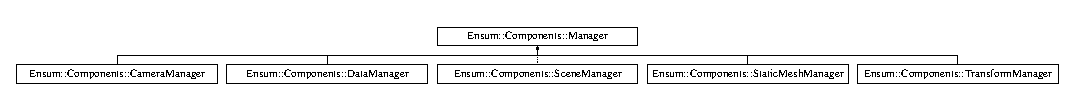
\includegraphics[height=0.892430cm]{class_ensum_1_1_components_1_1_manager}
\end{center}
\end{figure}
\subsection*{Classes}
\begin{DoxyCompactItemize}
\item 
struct \hyperlink{struct_ensum_1_1_components_1_1_manager_1_1_manager_meta_data}{Manager\+Meta\+Data}
\begin{DoxyCompactList}\small\item\em The minimum data that all managers has to keep. \end{DoxyCompactList}\end{DoxyCompactItemize}
\subsection*{Public Member Functions}
\begin{DoxyCompactItemize}
\item 
virtual const void \hyperlink{class_ensum_1_1_components_1_1_manager_a7327f9a28abf0011498ced0c86692a73}{Frame} ()\hypertarget{class_ensum_1_1_components_1_1_manager_a7327f9a28abf0011498ced0c86692a73}{}\label{class_ensum_1_1_components_1_1_manager_a7327f9a28abf0011498ced0c86692a73}

\begin{DoxyCompactList}\small\item\em Do the framework for all active scenes. \end{DoxyCompactList}\item 
virtual const void \hyperlink{class_ensum_1_1_components_1_1_manager_a3be559f70a5fc91769be008493948d61}{Destroy} (const \hyperlink{struct_ensum_1_1_components_1_1_entity}{Entity} \&entity)\hypertarget{class_ensum_1_1_components_1_1_manager_a3be559f70a5fc91769be008493948d61}{}\label{class_ensum_1_1_components_1_1_manager_a3be559f70a5fc91769be008493948d61}

\begin{DoxyCompactList}\small\item\em Public destroy function. \end{DoxyCompactList}\end{DoxyCompactItemize}
\subsection*{Protected Member Functions}
\begin{DoxyCompactItemize}
\item 
\hyperlink{class_ensum_1_1_components_1_1_manager_ab75b75d4c5936733c4af3840a4fc7f5c}{Manager} (\hyperlink{struct_ensum_1_1_components_1_1_manager_1_1_manager_meta_data}{Manager\+Meta\+Data} $\ast$data, \hyperlink{class_ensum_1_1_components_1_1_entity_manager}{Entity\+Manager} \&ent\+Manager)
\begin{DoxyCompactList}\small\item\em The constructor. \end{DoxyCompactList}\item 
virtual const void \hyperlink{class_ensum_1_1_components_1_1_manager_a1b593059210d09632c910a6abaae49c0}{\+\_\+\+Allocate} (uint32\+\_\+t size)=0
\begin{DoxyCompactList}\small\item\em Allocate more memory for scenedata. \end{DoxyCompactList}\item 
virtual const void \hyperlink{class_ensum_1_1_components_1_1_manager_a5ba85395802e942ed8904ca18951e6b0}{\+\_\+\+Destroy} (uint32\+\_\+t index)=0
\begin{DoxyCompactList}\small\item\em Delete an entry in the memory block. \end{DoxyCompactList}\item 
virtual const void \hyperlink{class_ensum_1_1_components_1_1_manager_a646aca9437267a1da465862ba7cc77a3}{\+\_\+\+GC} ()\hypertarget{class_ensum_1_1_components_1_1_manager_a646aca9437267a1da465862ba7cc77a3}{}\label{class_ensum_1_1_components_1_1_manager_a646aca9437267a1da465862ba7cc77a3}

\begin{DoxyCompactList}\small\item\em Looks for destroyed entities and deletes them from the data block. \end{DoxyCompactList}\end{DoxyCompactItemize}
\subsection*{Protected Attributes}
\begin{DoxyCompactItemize}
\item 
std\+::default\+\_\+random\+\_\+engine {\bfseries \+\_\+generator}\hypertarget{class_ensum_1_1_components_1_1_manager_aea13da4e297ed8c902ec32ef074e3e70}{}\label{class_ensum_1_1_components_1_1_manager_aea13da4e297ed8c902ec32ef074e3e70}

\item 
std\+::unordered\+\_\+map$<$ \hyperlink{struct_ensum_1_1_components_1_1_entity}{Entity}, uint32\+\_\+t, \hyperlink{struct_ensum_1_1_components_1_1_entity_hasher}{Entity\+Hasher} $>$ $\ast$ {\bfseries \+\_\+entity\+To\+Index}\hypertarget{class_ensum_1_1_components_1_1_manager_a60e97a2c011d3fae42b2a7e36bd0ffb8}{}\label{class_ensum_1_1_components_1_1_manager_a60e97a2c011d3fae42b2a7e36bd0ffb8}

\item 
\hyperlink{struct_ensum_1_1_components_1_1_manager_1_1_manager_meta_data}{Manager\+Meta\+Data} $\ast$ {\bfseries \+\_\+data}\hypertarget{class_ensum_1_1_components_1_1_manager_a6ff9f92350f25612b092e0330941a8e4}{}\label{class_ensum_1_1_components_1_1_manager_a6ff9f92350f25612b092e0330941a8e4}

\item 
\hyperlink{class_ensum_1_1_components_1_1_entity_manager}{Entity\+Manager} \& {\bfseries \+\_\+entity\+Manager}\hypertarget{class_ensum_1_1_components_1_1_manager_a24f14f5ffe72655f9183283a98e3a0a3}{}\label{class_ensum_1_1_components_1_1_manager_a24f14f5ffe72655f9183283a98e3a0a3}

\end{DoxyCompactItemize}


\subsection{Detailed Description}
Fully virtual base manager class. 

This is to enforce the structure of the managers. 

\subsection{Constructor \& Destructor Documentation}
\index{Ensum\+::\+Components\+::\+Manager@{Ensum\+::\+Components\+::\+Manager}!Manager@{Manager}}
\index{Manager@{Manager}!Ensum\+::\+Components\+::\+Manager@{Ensum\+::\+Components\+::\+Manager}}
\subsubsection[{\texorpdfstring{Manager(\+Manager\+Meta\+Data $\ast$data, Entity\+Manager \&ent\+Manager)}{Manager(ManagerMetaData *data, EntityManager &entManager)}}]{\setlength{\rightskip}{0pt plus 5cm}Ensum\+::\+Components\+::\+Manager\+::\+Manager (
\begin{DoxyParamCaption}
\item[{{\bf Manager\+Meta\+Data} $\ast$}]{data, }
\item[{{\bf Entity\+Manager} \&}]{ent\+Manager}
\end{DoxyParamCaption}
)\hspace{0.3cm}{\ttfamily [inline]}, {\ttfamily [protected]}}\hypertarget{class_ensum_1_1_components_1_1_manager_ab75b75d4c5936733c4af3840a4fc7f5c}{}\label{class_ensum_1_1_components_1_1_manager_ab75b75d4c5936733c4af3840a4fc7f5c}


The constructor. 

The data pointer is the specific managers own struct. (Created with new). 

\subsection{Member Function Documentation}
\index{Ensum\+::\+Components\+::\+Manager@{Ensum\+::\+Components\+::\+Manager}!\+\_\+\+Allocate@{\+\_\+\+Allocate}}
\index{\+\_\+\+Allocate@{\+\_\+\+Allocate}!Ensum\+::\+Components\+::\+Manager@{Ensum\+::\+Components\+::\+Manager}}
\subsubsection[{\texorpdfstring{\+\_\+\+Allocate(uint32\+\_\+t size)=0}{_Allocate(uint32_t size)=0}}]{\setlength{\rightskip}{0pt plus 5cm}virtual const void Ensum\+::\+Components\+::\+Manager\+::\+\_\+\+Allocate (
\begin{DoxyParamCaption}
\item[{uint32\+\_\+t}]{size}
\end{DoxyParamCaption}
)\hspace{0.3cm}{\ttfamily [protected]}, {\ttfamily [pure virtual]}}\hypertarget{class_ensum_1_1_components_1_1_manager_a1b593059210d09632c910a6abaae49c0}{}\label{class_ensum_1_1_components_1_1_manager_a1b593059210d09632c910a6abaae49c0}


Allocate more memory for scenedata. 



Implemented in \hyperlink{class_ensum_1_1_components_1_1_data_manager_aa9f344da59b7fda790b79a9e453ba7c4}{Ensum\+::\+Components\+::\+Data\+Manager}, \hyperlink{class_ensum_1_1_components_1_1_transform_manager_a90703a5b97caaafee225459ca872c446}{Ensum\+::\+Components\+::\+Transform\+Manager}, \hyperlink{class_ensum_1_1_components_1_1_camera_manager_a1ccb090150e77084806fa903bc5006e5}{Ensum\+::\+Components\+::\+Camera\+Manager}, \hyperlink{class_ensum_1_1_components_1_1_scene_manager_a383a468319c93280ce8ac0bbb920ab87}{Ensum\+::\+Components\+::\+Scene\+Manager}, and \hyperlink{class_ensum_1_1_components_1_1_static_mesh_manager_a470c7fb98f91c55b803ef8d2dd7a4803}{Ensum\+::\+Components\+::\+Static\+Mesh\+Manager}.

\index{Ensum\+::\+Components\+::\+Manager@{Ensum\+::\+Components\+::\+Manager}!\+\_\+\+Destroy@{\+\_\+\+Destroy}}
\index{\+\_\+\+Destroy@{\+\_\+\+Destroy}!Ensum\+::\+Components\+::\+Manager@{Ensum\+::\+Components\+::\+Manager}}
\subsubsection[{\texorpdfstring{\+\_\+\+Destroy(uint32\+\_\+t index)=0}{_Destroy(uint32_t index)=0}}]{\setlength{\rightskip}{0pt plus 5cm}virtual const void Ensum\+::\+Components\+::\+Manager\+::\+\_\+\+Destroy (
\begin{DoxyParamCaption}
\item[{uint32\+\_\+t}]{index}
\end{DoxyParamCaption}
)\hspace{0.3cm}{\ttfamily [protected]}, {\ttfamily [pure virtual]}}\hypertarget{class_ensum_1_1_components_1_1_manager_a5ba85395802e942ed8904ca18951e6b0}{}\label{class_ensum_1_1_components_1_1_manager_a5ba85395802e942ed8904ca18951e6b0}


Delete an entry in the memory block. 

The deleted entry is replaced by the last in the block. 

Implemented in \hyperlink{class_ensum_1_1_components_1_1_data_manager_a6f5c2ed92eba2cb4d5c15c451cbf089c}{Ensum\+::\+Components\+::\+Data\+Manager}, \hyperlink{class_ensum_1_1_components_1_1_transform_manager_a47f354c8a26b83d12809611516be65c7}{Ensum\+::\+Components\+::\+Transform\+Manager}, \hyperlink{class_ensum_1_1_components_1_1_camera_manager_a7a4aff38cf9e0fa2d504e0836d06efe7}{Ensum\+::\+Components\+::\+Camera\+Manager}, \hyperlink{class_ensum_1_1_components_1_1_scene_manager_a8102cfd9f4fed62a06e564dc016b6c46}{Ensum\+::\+Components\+::\+Scene\+Manager}, and \hyperlink{class_ensum_1_1_components_1_1_static_mesh_manager_a3d7684a00092ff8d467425a9f1ba7e5c}{Ensum\+::\+Components\+::\+Static\+Mesh\+Manager}.



The documentation for this class was generated from the following file\+:\begin{DoxyCompactItemize}
\item 
C\+:/\+Users/peter/\+Source/\+Repos/\+E\+N\+S\+U\+M/\+Ensum/\+Includes/\+Ensum\+\_\+components/Manager.\+h\end{DoxyCompactItemize}

\hypertarget{struct_ensum_1_1_components_1_1_manager_1_1_manager_meta_data}{}\section{Ensum\+:\+:Components\+:\+:Manager\+:\+:Manager\+Meta\+Data Struct Reference}
\label{struct_ensum_1_1_components_1_1_manager_1_1_manager_meta_data}\index{Ensum\+::\+Components\+::\+Manager\+::\+Manager\+Meta\+Data@{Ensum\+::\+Components\+::\+Manager\+::\+Manager\+Meta\+Data}}


The minimum data that all managers has to keep.  




{\ttfamily \#include $<$Manager.\+h$>$}

Inheritance diagram for Ensum\+:\+:Components\+:\+:Manager\+:\+:Manager\+Meta\+Data\+:\begin{figure}[H]
\begin{center}
\leavevmode
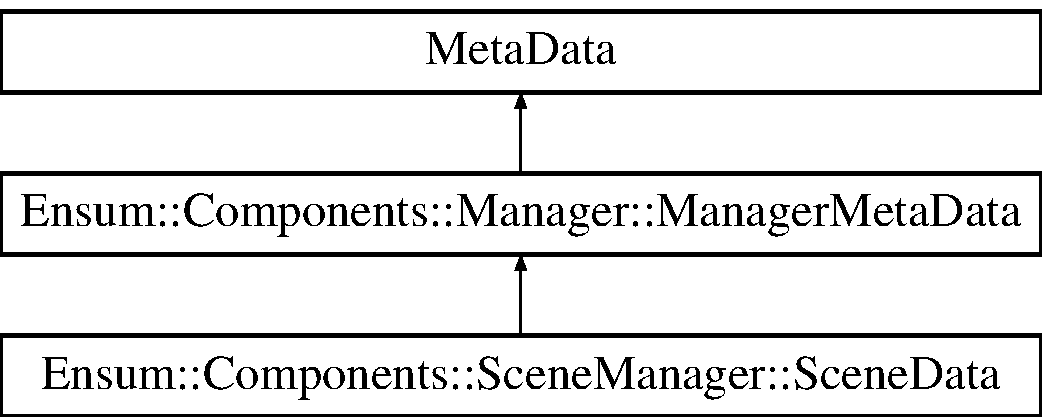
\includegraphics[height=3.000000cm]{struct_ensum_1_1_components_1_1_manager_1_1_manager_meta_data}
\end{center}
\end{figure}
\subsection*{Public Attributes}
\begin{DoxyCompactItemize}
\item 
\hyperlink{struct_ensum_1_1_components_1_1_entity}{Entity} $\ast$ {\bfseries entity}\hypertarget{struct_ensum_1_1_components_1_1_manager_1_1_manager_meta_data_ac7f0ba43f4aa9d1586e2ebc0f6b52276}{}\label{struct_ensum_1_1_components_1_1_manager_1_1_manager_meta_data_ac7f0ba43f4aa9d1586e2ebc0f6b52276}

\end{DoxyCompactItemize}


\subsection{Detailed Description}
The minimum data that all managers has to keep. 

When creating a manager inherit from this struct. 

The documentation for this struct was generated from the following file\+:\begin{DoxyCompactItemize}
\item 
Includes/\+Ensum\+\_\+components/Manager.\+h\end{DoxyCompactItemize}

\hypertarget{class_ensum_1_1_file_handler_1_1_mesh}{}\section{Ensum\+:\+:File\+Handler\+:\+:Mesh Class Reference}
\label{class_ensum_1_1_file_handler_1_1_mesh}\index{Ensum\+::\+File\+Handler\+::\+Mesh@{Ensum\+::\+File\+Handler\+::\+Mesh}}
\subsection*{Public Member Functions}
\begin{DoxyCompactItemize}
\item 
{\bfseries Mesh} (const char $\ast$path)\hypertarget{class_ensum_1_1_file_handler_1_1_mesh_a40a76db2b735e5939023f3fd9154cc07}{}\label{class_ensum_1_1_file_handler_1_1_mesh_a40a76db2b735e5939023f3fd9154cc07}

\item 
{\bfseries Mesh} (const \hyperlink{class_ensum_1_1_file_handler_1_1_mesh}{Mesh} \&other)\hypertarget{class_ensum_1_1_file_handler_1_1_mesh_ac3d565bc063a5c6881c3ae0d13aa3808}{}\label{class_ensum_1_1_file_handler_1_1_mesh_ac3d565bc063a5c6881c3ae0d13aa3808}

\end{DoxyCompactItemize}
\subsection*{Protected Attributes}
\begin{DoxyCompactItemize}
\item 
\hyperlink{struct_ensum_1_1_file_handler_1_1_data}{Data} {\bfseries \+\_\+data}\hypertarget{class_ensum_1_1_file_handler_1_1_mesh_ae2c87be19b8db4b742f5aee9e356d02b}{}\label{class_ensum_1_1_file_handler_1_1_mesh_ae2c87be19b8db4b742f5aee9e356d02b}

\end{DoxyCompactItemize}


The documentation for this class was generated from the following file\+:\begin{DoxyCompactItemize}
\item 
C\+:/\+Users/peter/\+Source/\+Repos/\+E\+N\+S\+U\+M/\+Ensum/\+Includes/\+Ensum\+\_\+filehandler/Mesh.\+h\end{DoxyCompactItemize}

\hypertarget{struct_ensum_1_1_components_1_1_static_mesh_manager_1_1_mesh_component}{}\section{Ensum\+:\+:Components\+:\+:Static\+Mesh\+Manager\+:\+:Mesh\+Component Struct Reference}
\label{struct_ensum_1_1_components_1_1_static_mesh_manager_1_1_mesh_component}\index{Ensum\+::\+Components\+::\+Static\+Mesh\+Manager\+::\+Mesh\+Component@{Ensum\+::\+Components\+::\+Static\+Mesh\+Manager\+::\+Mesh\+Component}}


The managers data struct.  


Inheritance diagram for Ensum\+:\+:Components\+:\+:Static\+Mesh\+Manager\+:\+:Mesh\+Component\+:\begin{figure}[H]
\begin{center}
\leavevmode
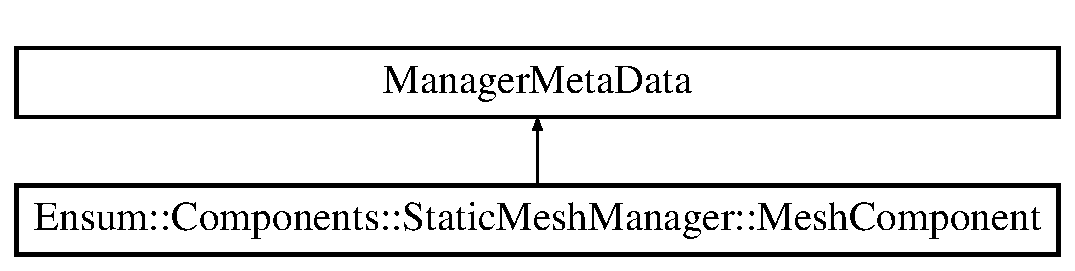
\includegraphics[height=2.000000cm]{struct_ensum_1_1_components_1_1_static_mesh_manager_1_1_mesh_component}
\end{center}
\end{figure}
\subsection*{Public Attributes}
\begin{DoxyCompactItemize}
\item 
uint32\+\_\+t $\ast$ {\bfseries buffer\+ID}\hypertarget{struct_ensum_1_1_components_1_1_static_mesh_manager_1_1_mesh_component_a3797586ec1e14a2108e36fe238638b44}{}\label{struct_ensum_1_1_components_1_1_static_mesh_manager_1_1_mesh_component_a3797586ec1e14a2108e36fe238638b44}

\item 
uint32\+\_\+t $\ast$ {\bfseries num\+Sub\+Meshes}\hypertarget{struct_ensum_1_1_components_1_1_static_mesh_manager_1_1_mesh_component_a44f17e361b43b8ececaf97f320cc8ed9}{}\label{struct_ensum_1_1_components_1_1_static_mesh_manager_1_1_mesh_component_a44f17e361b43b8ececaf97f320cc8ed9}

\item 
uint64\+\_\+t $\ast$$\ast$ {\bfseries index\+Start}\hypertarget{struct_ensum_1_1_components_1_1_static_mesh_manager_1_1_mesh_component_ab03342643178c69d0c04b88b0af738cb}{}\label{struct_ensum_1_1_components_1_1_static_mesh_manager_1_1_mesh_component_ab03342643178c69d0c04b88b0af738cb}

\item 
uint64\+\_\+t $\ast$$\ast$ {\bfseries index\+Count}\hypertarget{struct_ensum_1_1_components_1_1_static_mesh_manager_1_1_mesh_component_a8a4a39ae87a62004985ca73238e9896a}{}\label{struct_ensum_1_1_components_1_1_static_mesh_manager_1_1_mesh_component_a8a4a39ae87a62004985ca73238e9896a}

\item 
bool $\ast$$\ast$ {\bfseries visible}\hypertarget{struct_ensum_1_1_components_1_1_static_mesh_manager_1_1_mesh_component_a83491ddc3b2880efcdcdb22b761606ec}{}\label{struct_ensum_1_1_components_1_1_static_mesh_manager_1_1_mesh_component_a83491ddc3b2880efcdcdb22b761606ec}

\end{DoxyCompactItemize}


\subsection{Detailed Description}
The managers data struct. 

The documentation for this struct was generated from the following file\+:\begin{DoxyCompactItemize}
\item 
C\+:/\+Users/peter/\+Source/\+Repos/\+E\+N\+S\+U\+M/\+Ensum/\+Includes/\+Ensum\+\_\+components/Static\+Mesh\+Manager.\+h\end{DoxyCompactItemize}

\hypertarget{struct_ensum_1_1_file_handler_1_1_mesh_data}{}\section{Ensum\+:\+:File\+Handler\+:\+:Mesh\+Data Struct Reference}
\label{struct_ensum_1_1_file_handler_1_1_mesh_data}\index{Ensum\+::\+File\+Handler\+::\+Mesh\+Data@{Ensum\+::\+File\+Handler\+::\+Mesh\+Data}}
\subsection*{Public Member Functions}
\begin{DoxyCompactItemize}
\item 
{\bfseries Mesh\+Data} (const \hyperlink{struct_ensum_1_1_file_handler_1_1_mesh_data}{Mesh\+Data} \&other)\hypertarget{struct_ensum_1_1_file_handler_1_1_mesh_data_a2860e91af617fb3be7145acd3ab3ac90}{}\label{struct_ensum_1_1_file_handler_1_1_mesh_data_a2860e91af617fb3be7145acd3ab3ac90}

\item 
\hyperlink{struct_ensum_1_1_file_handler_1_1_mesh_data}{Mesh\+Data} \& {\bfseries operator=} (const \hyperlink{struct_ensum_1_1_file_handler_1_1_mesh_data}{Mesh\+Data} \&other)\hypertarget{struct_ensum_1_1_file_handler_1_1_mesh_data_a82b70f364ae3e8e2abeab1f7372069f9}{}\label{struct_ensum_1_1_file_handler_1_1_mesh_data_a82b70f364ae3e8e2abeab1f7372069f9}

\end{DoxyCompactItemize}
\subsection*{Public Attributes}
\begin{DoxyCompactItemize}
\item 
uint32\+\_\+t {\bfseries buffer\+ID}\hypertarget{struct_ensum_1_1_file_handler_1_1_mesh_data_a9363dc6018bd3866bef535efba7de0e2}{}\label{struct_ensum_1_1_file_handler_1_1_mesh_data_a9363dc6018bd3866bef535efba7de0e2}

\item 
uint32\+\_\+t {\bfseries num\+Sub\+Meshes}\hypertarget{struct_ensum_1_1_file_handler_1_1_mesh_data_aebcda9f23d590970590dfe144131dc0f}{}\label{struct_ensum_1_1_file_handler_1_1_mesh_data_aebcda9f23d590970590dfe144131dc0f}

\item 
uint64\+\_\+t $\ast$ {\bfseries index\+Start}\hypertarget{struct_ensum_1_1_file_handler_1_1_mesh_data_a62448a9ab27473cfc6649c515fb4248d}{}\label{struct_ensum_1_1_file_handler_1_1_mesh_data_a62448a9ab27473cfc6649c515fb4248d}

\item 
uint64\+\_\+t $\ast$ {\bfseries index\+Count}\hypertarget{struct_ensum_1_1_file_handler_1_1_mesh_data_a406c6cfb40639a760121d6ccb0c5cab9}{}\label{struct_ensum_1_1_file_handler_1_1_mesh_data_a406c6cfb40639a760121d6ccb0c5cab9}

\end{DoxyCompactItemize}


The documentation for this struct was generated from the following file\+:\begin{DoxyCompactItemize}
\item 
C\+:/\+Users/peter/\+Source/\+Repos/\+E\+N\+S\+U\+M/\+Ensum/\+Includes/\+Ensum\+\_\+filehandler/Mesh.\+h\end{DoxyCompactItemize}

\hypertarget{struct_meta_data}{}\section{Meta\+Data Struct Reference}
\label{struct_meta_data}\index{Meta\+Data@{Meta\+Data}}
Inheritance diagram for Meta\+Data\+:\begin{figure}[H]
\begin{center}
\leavevmode
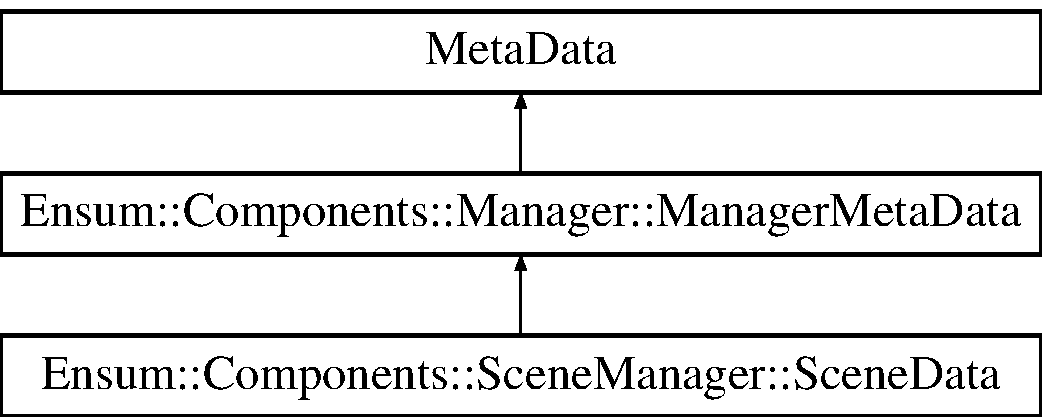
\includegraphics[height=3.000000cm]{struct_meta_data}
\end{center}
\end{figure}
\subsection*{Public Attributes}
\begin{DoxyCompactItemize}
\item 
uint32\+\_\+t {\bfseries used} = 0\hypertarget{struct_meta_data_abdcac78a4eaf9c6e69d4fdc0c0f1a1cf}{}\label{struct_meta_data_abdcac78a4eaf9c6e69d4fdc0c0f1a1cf}

\item 
uint32\+\_\+t {\bfseries allocated} = 0\hypertarget{struct_meta_data_ad7f915f404b7b1b3d46a19b0fa6f9a0c}{}\label{struct_meta_data_ad7f915f404b7b1b3d46a19b0fa6f9a0c}

\item 
void $\ast$ {\bfseries buffer} = nullptr\hypertarget{struct_meta_data_a3d09d759d39ddf22e23b3783d82b1c68}{}\label{struct_meta_data_a3d09d759d39ddf22e23b3783d82b1c68}

\end{DoxyCompactItemize}


The documentation for this struct was generated from the following file\+:\begin{DoxyCompactItemize}
\item 
C\+:/\+Users/peter/\+Source/\+Repos/\+E\+N\+S\+U\+M/\+Ensum/\+Includes/Data\+\_\+\+Meta.\+h\end{DoxyCompactItemize}

\hypertarget{struct_ensum_1_1_file_handler_1_1_normal}{}\section{Ensum\+:\+:File\+Handler\+:\+:Normal Struct Reference}
\label{struct_ensum_1_1_file_handler_1_1_normal}\index{Ensum\+::\+File\+Handler\+::\+Normal@{Ensum\+::\+File\+Handler\+::\+Normal}}
\subsection*{Public Member Functions}
\begin{DoxyCompactItemize}
\item 
{\bfseries Normal} (float x, float y, float z)\hypertarget{struct_ensum_1_1_file_handler_1_1_normal_adca8172078729f3e4803e0815804f44a}{}\label{struct_ensum_1_1_file_handler_1_1_normal_adca8172078729f3e4803e0815804f44a}

\end{DoxyCompactItemize}
\subsection*{Public Attributes}
\begin{DoxyCompactItemize}
\item 
float {\bfseries x}\hypertarget{struct_ensum_1_1_file_handler_1_1_normal_a4688ba702c53c978c6f3a581d80c24e2}{}\label{struct_ensum_1_1_file_handler_1_1_normal_a4688ba702c53c978c6f3a581d80c24e2}

\item 
float {\bfseries y}\hypertarget{struct_ensum_1_1_file_handler_1_1_normal_aa392a1dd171ff86ef4c537c9ea4c8fda}{}\label{struct_ensum_1_1_file_handler_1_1_normal_aa392a1dd171ff86ef4c537c9ea4c8fda}

\item 
float {\bfseries z}\hypertarget{struct_ensum_1_1_file_handler_1_1_normal_a1df535481db8e52b93f0b365313c2ca2}{}\label{struct_ensum_1_1_file_handler_1_1_normal_a1df535481db8e52b93f0b365313c2ca2}

\end{DoxyCompactItemize}


The documentation for this struct was generated from the following file\+:\begin{DoxyCompactItemize}
\item 
C\+:/\+Users/peter/\+Source/\+Repos/\+E\+N\+S\+U\+M/\+Ensum/\+Includes/\+Ensum\+\_\+filehandler/Mesh.\+h\end{DoxyCompactItemize}

\hypertarget{class_ensum_1_1_components_1_1_null_scene}{}\section{Ensum\+:\+:Components\+:\+:Null\+Scene Class Reference}
\label{class_ensum_1_1_components_1_1_null_scene}\index{Ensum\+::\+Components\+::\+Null\+Scene@{Ensum\+::\+Components\+::\+Null\+Scene}}


A scene that does nothing.  




{\ttfamily \#include $<$Null\+Scene.\+h$>$}

Inheritance diagram for Ensum\+:\+:Components\+:\+:Null\+Scene\+:\begin{figure}[H]
\begin{center}
\leavevmode
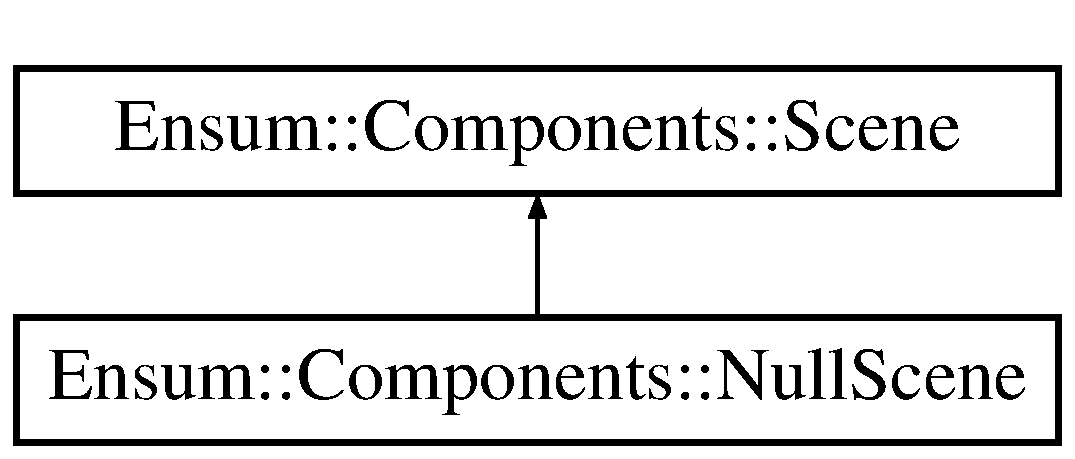
\includegraphics[height=2.000000cm]{class_ensum_1_1_components_1_1_null_scene}
\end{center}
\end{figure}
\subsection*{Public Member Functions}
\begin{DoxyCompactItemize}
\item 
{\bfseries Null\+Scene} (\hyperlink{class_ensum_1_1_components_1_1_entity_manager}{Entity\+Manager} \&entity\+Manger, \hyperlink{class_ensum_1_1_input_1_1_input}{Input\+::\+Input} $\ast$input)\hypertarget{class_ensum_1_1_components_1_1_null_scene_a140c16207aa1450a50a78bd4030cffb4}{}\label{class_ensum_1_1_components_1_1_null_scene_a140c16207aa1450a50a78bd4030cffb4}

\end{DoxyCompactItemize}
\subsection*{Additional Inherited Members}


\subsection{Detailed Description}
A scene that does nothing. 

The documentation for this class was generated from the following file\+:\begin{DoxyCompactItemize}
\item 
C\+:/\+Users/peter/\+Source/\+Repos/\+E\+N\+S\+U\+M/\+Ensum/\+Includes/\+Ensum\+\_\+components/Null\+Scene.\+h\end{DoxyCompactItemize}

\hypertarget{class_ensum_1_1_utils_1_1_options}{}\section{Ensum\+:\+:Utils\+:\+:Options Class Reference}
\label{class_ensum_1_1_utils_1_1_options}\index{Ensum\+::\+Utils\+::\+Options@{Ensum\+::\+Utils\+::\+Options}}


A singleton class for reading and writing to config file.  




{\ttfamily \#include $<$Options.\+h$>$}

\subsection*{Static Public Member Functions}
\begin{DoxyCompactItemize}
\item 
static E\+N\+S\+U\+M\+\_\+\+U\+T\+I\+L\+S\+\_\+\+E\+X\+P\+O\+RT void \hyperlink{class_ensum_1_1_utils_1_1_options_a42cd72b90a957177404071c01bca1ea0}{Create\+Instance} ()
\begin{DoxyCompactList}\small\item\em Create the options instance. \end{DoxyCompactList}\item 
static E\+N\+S\+U\+M\+\_\+\+U\+T\+I\+L\+S\+\_\+\+E\+X\+P\+O\+RT void \hyperlink{class_ensum_1_1_utils_1_1_options_ace3ea5450fca95ba36201463cb47c3da}{Delete\+Instance} ()\hypertarget{class_ensum_1_1_utils_1_1_options_ace3ea5450fca95ba36201463cb47c3da}{}\label{class_ensum_1_1_utils_1_1_options_ace3ea5450fca95ba36201463cb47c3da}

\begin{DoxyCompactList}\small\item\em Deletes the instance. \end{DoxyCompactList}\item 
static E\+N\+S\+U\+M\+\_\+\+U\+T\+I\+L\+S\+\_\+\+E\+X\+P\+O\+RT long \hyperlink{class_ensum_1_1_utils_1_1_options_a784e8e989bea701170af8b689f040e90}{Get\+Integer\+Option} (const \hyperlink{class_ensum_1_1string}{string} \&section, const \hyperlink{class_ensum_1_1string}{string} \&option, long default\+\_\+value)\hypertarget{class_ensum_1_1_utils_1_1_options_a784e8e989bea701170af8b689f040e90}{}\label{class_ensum_1_1_utils_1_1_options_a784e8e989bea701170af8b689f040e90}

\begin{DoxyCompactList}\small\item\em Public read function. \end{DoxyCompactList}\item 
static E\+N\+S\+U\+M\+\_\+\+U\+T\+I\+L\+S\+\_\+\+E\+X\+P\+O\+RT double \hyperlink{class_ensum_1_1_utils_1_1_options_ac57c333c1f9bd66472fecaa8b7f55f30}{Get\+Real\+Option} (const \hyperlink{class_ensum_1_1string}{string} \&section, const \hyperlink{class_ensum_1_1string}{string} \&option, double default\+\_\+value)\hypertarget{class_ensum_1_1_utils_1_1_options_ac57c333c1f9bd66472fecaa8b7f55f30}{}\label{class_ensum_1_1_utils_1_1_options_ac57c333c1f9bd66472fecaa8b7f55f30}

\begin{DoxyCompactList}\small\item\em Public read function. \end{DoxyCompactList}\item 
static E\+N\+S\+U\+M\+\_\+\+U\+T\+I\+L\+S\+\_\+\+E\+X\+P\+O\+RT bool \hyperlink{class_ensum_1_1_utils_1_1_options_ad0925b8894344c6d4425fbf0acde3852}{Get\+Boolean\+Option} (const \hyperlink{class_ensum_1_1string}{string} \&section, const \hyperlink{class_ensum_1_1string}{string} \&option, bool default\+\_\+value)\hypertarget{class_ensum_1_1_utils_1_1_options_ad0925b8894344c6d4425fbf0acde3852}{}\label{class_ensum_1_1_utils_1_1_options_ad0925b8894344c6d4425fbf0acde3852}

\begin{DoxyCompactList}\small\item\em Public read function. \end{DoxyCompactList}\item 
static E\+N\+S\+U\+M\+\_\+\+U\+T\+I\+L\+S\+\_\+\+E\+X\+P\+O\+RT \hyperlink{class_ensum_1_1string}{string} \hyperlink{class_ensum_1_1_utils_1_1_options_ac89c9d4c8e4dde0a1b07745c97d082a9}{Get\+String\+Option} (const \hyperlink{class_ensum_1_1string}{string} \&section, const \hyperlink{class_ensum_1_1string}{string} \&option, const \hyperlink{class_ensum_1_1string}{string} \&default\+\_\+value)\hypertarget{class_ensum_1_1_utils_1_1_options_ac89c9d4c8e4dde0a1b07745c97d082a9}{}\label{class_ensum_1_1_utils_1_1_options_ac89c9d4c8e4dde0a1b07745c97d082a9}

\begin{DoxyCompactList}\small\item\em Public read function. \end{DoxyCompactList}\item 
static E\+N\+S\+U\+M\+\_\+\+U\+T\+I\+L\+S\+\_\+\+E\+X\+P\+O\+RT void \hyperlink{class_ensum_1_1_utils_1_1_options_a1d69b78fe5f4072908f5b615cd1ee9b4}{Set\+Integer\+Option} (const \hyperlink{class_ensum_1_1string}{string} \&section, const \hyperlink{class_ensum_1_1string}{string} \&option, long value)\hypertarget{class_ensum_1_1_utils_1_1_options_a1d69b78fe5f4072908f5b615cd1ee9b4}{}\label{class_ensum_1_1_utils_1_1_options_a1d69b78fe5f4072908f5b615cd1ee9b4}

\begin{DoxyCompactList}\small\item\em Public write function. \end{DoxyCompactList}\item 
static E\+N\+S\+U\+M\+\_\+\+U\+T\+I\+L\+S\+\_\+\+E\+X\+P\+O\+RT void \hyperlink{class_ensum_1_1_utils_1_1_options_ad8ebf2ce046cc95530f787bf372e7fd2}{Set\+Real\+Option} (const \hyperlink{class_ensum_1_1string}{string} \&section, const \hyperlink{class_ensum_1_1string}{string} \&option, double value)\hypertarget{class_ensum_1_1_utils_1_1_options_ad8ebf2ce046cc95530f787bf372e7fd2}{}\label{class_ensum_1_1_utils_1_1_options_ad8ebf2ce046cc95530f787bf372e7fd2}

\begin{DoxyCompactList}\small\item\em Public write function. \end{DoxyCompactList}\item 
static E\+N\+S\+U\+M\+\_\+\+U\+T\+I\+L\+S\+\_\+\+E\+X\+P\+O\+RT void \hyperlink{class_ensum_1_1_utils_1_1_options_a68837babb89a589bc49180fd849b2c28}{Set\+Boolean\+Option} (const \hyperlink{class_ensum_1_1string}{string} \&section, const \hyperlink{class_ensum_1_1string}{string} \&option, bool value)\hypertarget{class_ensum_1_1_utils_1_1_options_a68837babb89a589bc49180fd849b2c28}{}\label{class_ensum_1_1_utils_1_1_options_a68837babb89a589bc49180fd849b2c28}

\begin{DoxyCompactList}\small\item\em Public write function. \end{DoxyCompactList}\item 
static E\+N\+S\+U\+M\+\_\+\+U\+T\+I\+L\+S\+\_\+\+E\+X\+P\+O\+RT void \hyperlink{class_ensum_1_1_utils_1_1_options_a67df741524fdcd73f377d3b65f9699c9}{Set\+String\+Option} (const \hyperlink{class_ensum_1_1string}{string} \&section, const \hyperlink{class_ensum_1_1string}{string} \&option, const \hyperlink{class_ensum_1_1string}{string} \&value)\hypertarget{class_ensum_1_1_utils_1_1_options_a67df741524fdcd73f377d3b65f9699c9}{}\label{class_ensum_1_1_utils_1_1_options_a67df741524fdcd73f377d3b65f9699c9}

\begin{DoxyCompactList}\small\item\em Public write function. \end{DoxyCompactList}\item 
static E\+N\+S\+U\+M\+\_\+\+U\+T\+I\+L\+S\+\_\+\+E\+X\+P\+O\+RT void \hyperlink{class_ensum_1_1_utils_1_1_options_ab567217a53d2ef200574271fa3c957b1}{Subscribe} (\hyperlink{class_ensum_1_1_delegate}{Delegate}$<$ void()$>$ \&dele)
\begin{DoxyCompactList}\small\item\em Subscribe to the Options\+Change event. \end{DoxyCompactList}\item 
static E\+N\+S\+U\+M\+\_\+\+U\+T\+I\+L\+S\+\_\+\+E\+X\+P\+O\+RT void \hyperlink{class_ensum_1_1_utils_1_1_options_ac8945e45a27cd51401779bd92ae44fb2}{Un\+Subscribe} (\hyperlink{class_ensum_1_1_delegate}{Delegate}$<$ void()$>$ \&dele)\hypertarget{class_ensum_1_1_utils_1_1_options_ac8945e45a27cd51401779bd92ae44fb2}{}\label{class_ensum_1_1_utils_1_1_options_ac8945e45a27cd51401779bd92ae44fb2}

\begin{DoxyCompactList}\small\item\em Un\+Subscribe to the Options\+Change event. \end{DoxyCompactList}\end{DoxyCompactItemize}
\subsection*{Private Member Functions}
\begin{DoxyCompactItemize}
\item 
long \hyperlink{class_ensum_1_1_utils_1_1_options_a69b79cff0d5ad861b9f2be3bb296648f}{\+\_\+\+Get\+Integer\+Option} (const \hyperlink{class_ensum_1_1string}{string} \&section, const \hyperlink{class_ensum_1_1string}{string} \&option, long default\+\_\+value)\hypertarget{class_ensum_1_1_utils_1_1_options_a69b79cff0d5ad861b9f2be3bb296648f}{}\label{class_ensum_1_1_utils_1_1_options_a69b79cff0d5ad861b9f2be3bb296648f}

\begin{DoxyCompactList}\small\item\em Private Read function. \end{DoxyCompactList}\item 
double \hyperlink{class_ensum_1_1_utils_1_1_options_a3d79094def64e9e7bdbbe1c4532458e1}{\+\_\+\+Get\+Real\+Option} (const \hyperlink{class_ensum_1_1string}{string} \&section, const \hyperlink{class_ensum_1_1string}{string} \&option, double default\+\_\+value)\hypertarget{class_ensum_1_1_utils_1_1_options_a3d79094def64e9e7bdbbe1c4532458e1}{}\label{class_ensum_1_1_utils_1_1_options_a3d79094def64e9e7bdbbe1c4532458e1}

\begin{DoxyCompactList}\small\item\em Private Read function. \end{DoxyCompactList}\item 
bool \hyperlink{class_ensum_1_1_utils_1_1_options_a8c9a977bf971aa38af289af707a46490}{\+\_\+\+Get\+Boolean\+Option} (const \hyperlink{class_ensum_1_1string}{string} \&section, const \hyperlink{class_ensum_1_1string}{string} \&option, bool default\+\_\+value)\hypertarget{class_ensum_1_1_utils_1_1_options_a8c9a977bf971aa38af289af707a46490}{}\label{class_ensum_1_1_utils_1_1_options_a8c9a977bf971aa38af289af707a46490}

\begin{DoxyCompactList}\small\item\em Private Read function. \end{DoxyCompactList}\item 
\hyperlink{class_ensum_1_1string}{string} \hyperlink{class_ensum_1_1_utils_1_1_options_a741ecb0fda0375aa961d57108435c239}{\+\_\+\+Get\+String\+Option} (const \hyperlink{class_ensum_1_1string}{string} \&section, const \hyperlink{class_ensum_1_1string}{string} \&option, const \hyperlink{class_ensum_1_1string}{string} \&default\+\_\+value)\hypertarget{class_ensum_1_1_utils_1_1_options_a741ecb0fda0375aa961d57108435c239}{}\label{class_ensum_1_1_utils_1_1_options_a741ecb0fda0375aa961d57108435c239}

\begin{DoxyCompactList}\small\item\em Private Read function. \end{DoxyCompactList}\item 
void \hyperlink{class_ensum_1_1_utils_1_1_options_a8ed2a91a05fbabe8e83916adea5b2b96}{\+\_\+\+Set\+Integer\+Option} (const \hyperlink{class_ensum_1_1string}{string} \&section, const \hyperlink{class_ensum_1_1string}{string} \&option, long value)\hypertarget{class_ensum_1_1_utils_1_1_options_a8ed2a91a05fbabe8e83916adea5b2b96}{}\label{class_ensum_1_1_utils_1_1_options_a8ed2a91a05fbabe8e83916adea5b2b96}

\begin{DoxyCompactList}\small\item\em Private write function. \end{DoxyCompactList}\item 
void \hyperlink{class_ensum_1_1_utils_1_1_options_a1e6721c6556806ea91df7739c63e9ba2}{\+\_\+\+Set\+Real\+Option} (const \hyperlink{class_ensum_1_1string}{string} \&section, const \hyperlink{class_ensum_1_1string}{string} \&option, double value)\hypertarget{class_ensum_1_1_utils_1_1_options_a1e6721c6556806ea91df7739c63e9ba2}{}\label{class_ensum_1_1_utils_1_1_options_a1e6721c6556806ea91df7739c63e9ba2}

\begin{DoxyCompactList}\small\item\em Private write function. \end{DoxyCompactList}\item 
void \hyperlink{class_ensum_1_1_utils_1_1_options_ae7f2dc1a114d67fbe049454f6bb1aa1e}{\+\_\+\+Set\+Boolean\+Option} (const \hyperlink{class_ensum_1_1string}{string} \&section, const \hyperlink{class_ensum_1_1string}{string} \&option, bool value)\hypertarget{class_ensum_1_1_utils_1_1_options_ae7f2dc1a114d67fbe049454f6bb1aa1e}{}\label{class_ensum_1_1_utils_1_1_options_ae7f2dc1a114d67fbe049454f6bb1aa1e}

\begin{DoxyCompactList}\small\item\em Private write function. \end{DoxyCompactList}\item 
void \hyperlink{class_ensum_1_1_utils_1_1_options_a7ba0b31a187c20ffec4725b5f1fd9003}{\+\_\+\+Set\+String\+Option} (const \hyperlink{class_ensum_1_1string}{string} \&section, const \hyperlink{class_ensum_1_1string}{string} \&option, const \hyperlink{class_ensum_1_1string}{string} \&value)\hypertarget{class_ensum_1_1_utils_1_1_options_a7ba0b31a187c20ffec4725b5f1fd9003}{}\label{class_ensum_1_1_utils_1_1_options_a7ba0b31a187c20ffec4725b5f1fd9003}

\begin{DoxyCompactList}\small\item\em Private write function. \end{DoxyCompactList}\end{DoxyCompactItemize}
\subsection*{Private Attributes}
\begin{DoxyCompactItemize}
\item 
\hyperlink{class_ensum_1_1_file_handler_1_1ini}{File\+Handler\+::ini} $\ast$ {\bfseries \+\_\+file}\hypertarget{class_ensum_1_1_utils_1_1_options_ae10dba8ac3cb72c83e206ba2b74fa9c3}{}\label{class_ensum_1_1_utils_1_1_options_ae10dba8ac3cb72c83e206ba2b74fa9c3}

\item 
\hyperlink{class_ensum_1_1_event}{Event}$<$ void()$>$ {\bfseries \+\_\+\+Option\+Change}\hypertarget{class_ensum_1_1_utils_1_1_options_a8387d551a3972a8c09097fdc7b35c057}{}\label{class_ensum_1_1_utils_1_1_options_a8387d551a3972a8c09097fdc7b35c057}

\end{DoxyCompactItemize}
\subsection*{Static Private Attributes}
\begin{DoxyCompactItemize}
\item 
static \hyperlink{class_ensum_1_1_utils_1_1_options}{Options} $\ast$ {\bfseries \+\_\+instance}\hypertarget{class_ensum_1_1_utils_1_1_options_ade4681c12beae9f1acd240c4bdc2fb21}{}\label{class_ensum_1_1_utils_1_1_options_ade4681c12beae9f1acd240c4bdc2fb21}

\end{DoxyCompactItemize}


\subsection{Detailed Description}
A singleton class for reading and writing to config file. 

\subsection{Member Function Documentation}
\index{Ensum\+::\+Utils\+::\+Options@{Ensum\+::\+Utils\+::\+Options}!Create\+Instance@{Create\+Instance}}
\index{Create\+Instance@{Create\+Instance}!Ensum\+::\+Utils\+::\+Options@{Ensum\+::\+Utils\+::\+Options}}
\subsubsection[{\texorpdfstring{Create\+Instance()}{CreateInstance()}}]{\setlength{\rightskip}{0pt plus 5cm}static E\+N\+S\+U\+M\+\_\+\+U\+T\+I\+L\+S\+\_\+\+E\+X\+P\+O\+RT void Ensum\+::\+Utils\+::\+Options\+::\+Create\+Instance (
\begin{DoxyParamCaption}
{}
\end{DoxyParamCaption}
)\hspace{0.3cm}{\ttfamily [static]}}\hypertarget{class_ensum_1_1_utils_1_1_options_a42cd72b90a957177404071c01bca1ea0}{}\label{class_ensum_1_1_utils_1_1_options_a42cd72b90a957177404071c01bca1ea0}


Create the options instance. 

If options are not used all clients will simply use default values. \index{Ensum\+::\+Utils\+::\+Options@{Ensum\+::\+Utils\+::\+Options}!Subscribe@{Subscribe}}
\index{Subscribe@{Subscribe}!Ensum\+::\+Utils\+::\+Options@{Ensum\+::\+Utils\+::\+Options}}
\subsubsection[{\texorpdfstring{Subscribe(\+Delegate$<$ void()$>$ \&dele)}{Subscribe(Delegate< void()> &dele)}}]{\setlength{\rightskip}{0pt plus 5cm}static E\+N\+S\+U\+M\+\_\+\+U\+T\+I\+L\+S\+\_\+\+E\+X\+P\+O\+RT void Ensum\+::\+Utils\+::\+Options\+::\+Subscribe (
\begin{DoxyParamCaption}
\item[{{\bf Delegate}$<$ void()$>$ \&}]{dele}
\end{DoxyParamCaption}
)\hspace{0.3cm}{\ttfamily [static]}}\hypertarget{class_ensum_1_1_utils_1_1_options_ab567217a53d2ef200574271fa3c957b1}{}\label{class_ensum_1_1_utils_1_1_options_ab567217a53d2ef200574271fa3c957b1}


Subscribe to the Options\+Change event. 

When a change occurs in options this event is called. 

The documentation for this class was generated from the following file\+:\begin{DoxyCompactItemize}
\item 
Includes/\+Ensum\+\_\+utils/Options.\+h\end{DoxyCompactItemize}

\hypertarget{struct_ensum_1_1_file_handler_1_1_position}{}\section{Ensum\+:\+:File\+Handler\+:\+:Position Struct Reference}
\label{struct_ensum_1_1_file_handler_1_1_position}\index{Ensum\+::\+File\+Handler\+::\+Position@{Ensum\+::\+File\+Handler\+::\+Position}}
\subsection*{Public Member Functions}
\begin{DoxyCompactItemize}
\item 
{\bfseries Position} (float x, float y, float z, float w)\hypertarget{struct_ensum_1_1_file_handler_1_1_position_ae889f82eaa5ea4acb521c77c544067e4}{}\label{struct_ensum_1_1_file_handler_1_1_position_ae889f82eaa5ea4acb521c77c544067e4}

\end{DoxyCompactItemize}
\subsection*{Public Attributes}
\begin{DoxyCompactItemize}
\item 
float {\bfseries x}\hypertarget{struct_ensum_1_1_file_handler_1_1_position_a48dfb28fbf0223b9f7349921a2309f7f}{}\label{struct_ensum_1_1_file_handler_1_1_position_a48dfb28fbf0223b9f7349921a2309f7f}

\item 
float {\bfseries y}\hypertarget{struct_ensum_1_1_file_handler_1_1_position_ae0917114a009fb8c388f9a827a0f11c0}{}\label{struct_ensum_1_1_file_handler_1_1_position_ae0917114a009fb8c388f9a827a0f11c0}

\item 
float {\bfseries z}\hypertarget{struct_ensum_1_1_file_handler_1_1_position_a717ec95f14dca91bd146fca3e8bc9c56}{}\label{struct_ensum_1_1_file_handler_1_1_position_a717ec95f14dca91bd146fca3e8bc9c56}

\item 
float {\bfseries w}\hypertarget{struct_ensum_1_1_file_handler_1_1_position_adcd7ee30a2921e60cec18e41a5efdbd4}{}\label{struct_ensum_1_1_file_handler_1_1_position_adcd7ee30a2921e60cec18e41a5efdbd4}

\end{DoxyCompactItemize}


The documentation for this struct was generated from the following file\+:\begin{DoxyCompactItemize}
\item 
C\+:/\+Users/peter/\+Source/\+Repos/\+E\+N\+S\+U\+M/\+Ensum/\+Includes/\+Ensum\+\_\+filehandler/Mesh.\+h\end{DoxyCompactItemize}

\hypertarget{struct_ensum_1_1_graphics_1_1_rasterizer_state}{}\section{Ensum\+:\+:Graphics\+:\+:Rasterizer\+State Struct Reference}
\label{struct_ensum_1_1_graphics_1_1_rasterizer_state}\index{Ensum\+::\+Graphics\+::\+Rasterizer\+State@{Ensum\+::\+Graphics\+::\+Rasterizer\+State}}
\subsection*{Public Attributes}
\begin{DoxyCompactItemize}
\item 
I\+D3\+D11\+Rasterizer\+State $\ast$ {\bfseries RS} = nullptr\hypertarget{struct_ensum_1_1_graphics_1_1_rasterizer_state_ae3ef20a74ab9418142c0e4002c1b5c90}{}\label{struct_ensum_1_1_graphics_1_1_rasterizer_state_ae3ef20a74ab9418142c0e4002c1b5c90}

\item 
D3\+D11\+\_\+\+F\+I\+L\+L\+\_\+\+M\+O\+DE {\bfseries fill\+Mode} = D3\+D11\+\_\+\+F\+I\+L\+L\+\_\+\+S\+O\+L\+ID\hypertarget{struct_ensum_1_1_graphics_1_1_rasterizer_state_a265bb98074a662ab864eb5b2ff44e96b}{}\label{struct_ensum_1_1_graphics_1_1_rasterizer_state_a265bb98074a662ab864eb5b2ff44e96b}

\item 
D3\+D11\+\_\+\+C\+U\+L\+L\+\_\+\+M\+O\+DE {\bfseries cull\+Mode} = D3\+D11\+\_\+\+C\+U\+L\+L\+\_\+\+B\+A\+CK\hypertarget{struct_ensum_1_1_graphics_1_1_rasterizer_state_aca0a2f0d9dfad54792f66b3718a4d77d}{}\label{struct_ensum_1_1_graphics_1_1_rasterizer_state_aca0a2f0d9dfad54792f66b3718a4d77d}

\item 
bool {\bfseries front\+Counter\+Clockwise} = true\hypertarget{struct_ensum_1_1_graphics_1_1_rasterizer_state_a0ff4a89ecdf6bbfd726a8b35688f84b0}{}\label{struct_ensum_1_1_graphics_1_1_rasterizer_state_a0ff4a89ecdf6bbfd726a8b35688f84b0}

\item 
bool {\bfseries depth\+Bias} = false\hypertarget{struct_ensum_1_1_graphics_1_1_rasterizer_state_aba59a9d776f4dbe6bb121bc41e49392b}{}\label{struct_ensum_1_1_graphics_1_1_rasterizer_state_aba59a9d776f4dbe6bb121bc41e49392b}

\item 
float {\bfseries depth\+Bias\+Clamp} = 0.\+0f\hypertarget{struct_ensum_1_1_graphics_1_1_rasterizer_state_a10d339c084553ca221a82e7bbff677ad}{}\label{struct_ensum_1_1_graphics_1_1_rasterizer_state_a10d339c084553ca221a82e7bbff677ad}

\item 
float {\bfseries slope\+Scaled\+Depth\+Bias} = 0.\+0f\hypertarget{struct_ensum_1_1_graphics_1_1_rasterizer_state_ac4d7231b258bd51fc0fcdd5630cf4f18}{}\label{struct_ensum_1_1_graphics_1_1_rasterizer_state_ac4d7231b258bd51fc0fcdd5630cf4f18}

\item 
bool {\bfseries depth\+Clip\+Enable} = true\hypertarget{struct_ensum_1_1_graphics_1_1_rasterizer_state_a15a556ba8cfeff48b1d3aca4b956348a}{}\label{struct_ensum_1_1_graphics_1_1_rasterizer_state_a15a556ba8cfeff48b1d3aca4b956348a}

\item 
bool {\bfseries scissor\+Enable} = false\hypertarget{struct_ensum_1_1_graphics_1_1_rasterizer_state_a082afb9e60ba598f4416cdff9ab9475b}{}\label{struct_ensum_1_1_graphics_1_1_rasterizer_state_a082afb9e60ba598f4416cdff9ab9475b}

\item 
bool {\bfseries multi\+Sample\+Enable} = false\hypertarget{struct_ensum_1_1_graphics_1_1_rasterizer_state_ae538f865953bea7ef9fbde74dd686807}{}\label{struct_ensum_1_1_graphics_1_1_rasterizer_state_ae538f865953bea7ef9fbde74dd686807}

\item 
bool {\bfseries antialiased\+Line\+Enable} = false\hypertarget{struct_ensum_1_1_graphics_1_1_rasterizer_state_a22219a6c61777df7983ad4a4eb4b7381}{}\label{struct_ensum_1_1_graphics_1_1_rasterizer_state_a22219a6c61777df7983ad4a4eb4b7381}

\end{DoxyCompactItemize}


The documentation for this struct was generated from the following file\+:\begin{DoxyCompactItemize}
\item 
C\+:/\+Users/peter/\+Source/\+Repos/\+E\+N\+S\+U\+M/\+Ensum/\+Includes/\+Ensum\+\_\+graphics/Direct3\+D11.\+h\end{DoxyCompactItemize}

\hypertarget{struct_ensum_1_1_graphics_1_1_render_target}{}\section{Ensum\+:\+:Graphics\+:\+:Render\+Target Struct Reference}
\label{struct_ensum_1_1_graphics_1_1_render_target}\index{Ensum\+::\+Graphics\+::\+Render\+Target@{Ensum\+::\+Graphics\+::\+Render\+Target}}
\subsection*{Public Attributes}
\begin{DoxyCompactItemize}
\item 
I\+D3\+D11\+Resource $\ast$ {\bfseries Texture} = nullptr\hypertarget{struct_ensum_1_1_graphics_1_1_render_target_ad4052d607c6775f4b4a9610880240e95}{}\label{struct_ensum_1_1_graphics_1_1_render_target_ad4052d607c6775f4b4a9610880240e95}

\item 
I\+D3\+D11\+Render\+Target\+View $\ast$ {\bfseries R\+TV} = nullptr\hypertarget{struct_ensum_1_1_graphics_1_1_render_target_a150d9f216a511dcd7b618e844ffea07f}{}\label{struct_ensum_1_1_graphics_1_1_render_target_a150d9f216a511dcd7b618e844ffea07f}

\item 
I\+D3\+D11\+Shader\+Resource\+View $\ast$ {\bfseries S\+RV} = nullptr\hypertarget{struct_ensum_1_1_graphics_1_1_render_target_aab964884c66eb48bd47b6a5002b7be75}{}\label{struct_ensum_1_1_graphics_1_1_render_target_aab964884c66eb48bd47b6a5002b7be75}

\item 
I\+D3\+D11\+Unordered\+Access\+View $\ast$ {\bfseries U\+AV} = nullptr\hypertarget{struct_ensum_1_1_graphics_1_1_render_target_a39d871cac6b55eadaed7ca40216f98e3}{}\label{struct_ensum_1_1_graphics_1_1_render_target_a39d871cac6b55eadaed7ca40216f98e3}

\item 
I\+D3\+D11\+Render\+Target\+View $\ast$$\ast$ {\bfseries R\+T\+V\+Slices} = nullptr\hypertarget{struct_ensum_1_1_graphics_1_1_render_target_afcb061b38ef95e6466f8a5552ee5cb86}{}\label{struct_ensum_1_1_graphics_1_1_render_target_afcb061b38ef95e6466f8a5552ee5cb86}

\item 
I\+D3\+D11\+Shader\+Resource\+View $\ast$$\ast$ {\bfseries S\+R\+V\+Slices} = nullptr\hypertarget{struct_ensum_1_1_graphics_1_1_render_target_afd021f57acf98cdc1ca44ae41718de09}{}\label{struct_ensum_1_1_graphics_1_1_render_target_afd021f57acf98cdc1ca44ae41718de09}

\item 
I\+D3\+D11\+Unordered\+Access\+View $\ast$$\ast$ {\bfseries U\+A\+V\+Slices} = nullptr\hypertarget{struct_ensum_1_1_graphics_1_1_render_target_a09270a16a75d83656f7d93471b4ba955}{}\label{struct_ensum_1_1_graphics_1_1_render_target_a09270a16a75d83656f7d93471b4ba955}

\item 
unsigned {\bfseries Slice\+Count} = 1\hypertarget{struct_ensum_1_1_graphics_1_1_render_target_a1d4948952eb3ce8fd016974601f56699}{}\label{struct_ensum_1_1_graphics_1_1_render_target_a1d4948952eb3ce8fd016974601f56699}

\item 
D\+X\+G\+I\+\_\+\+F\+O\+R\+M\+AT {\bfseries Format} = D\+X\+G\+I\+\_\+\+F\+O\+R\+M\+A\+T\+\_\+\+U\+N\+K\+N\+O\+WN\hypertarget{struct_ensum_1_1_graphics_1_1_render_target_a1c5a451b1de1dee8d32fd8cbfa6eb143}{}\label{struct_ensum_1_1_graphics_1_1_render_target_a1c5a451b1de1dee8d32fd8cbfa6eb143}

\item 
unsigned {\bfseries Width} = 0\hypertarget{struct_ensum_1_1_graphics_1_1_render_target_ae12ebc14fb72f280410150d3d0ce63b1}{}\label{struct_ensum_1_1_graphics_1_1_render_target_ae12ebc14fb72f280410150d3d0ce63b1}

\item 
unsigned {\bfseries Height} = 0\hypertarget{struct_ensum_1_1_graphics_1_1_render_target_a5c4a5e9e8706576a7f16a338f1e55de2}{}\label{struct_ensum_1_1_graphics_1_1_render_target_a5c4a5e9e8706576a7f16a338f1e55de2}

\item 
unsigned {\bfseries Depth} = 0\hypertarget{struct_ensum_1_1_graphics_1_1_render_target_a6a4e846256b48d790217684150e2d295}{}\label{struct_ensum_1_1_graphics_1_1_render_target_a6a4e846256b48d790217684150e2d295}

\item 
unsigned {\bfseries Array\+Size} = 1\hypertarget{struct_ensum_1_1_graphics_1_1_render_target_ae6a4cdc4f51358aeeccaa334d57e845e}{}\label{struct_ensum_1_1_graphics_1_1_render_target_ae6a4cdc4f51358aeeccaa334d57e845e}

\item 
unsigned {\bfseries Mip\+Levels} = 1\hypertarget{struct_ensum_1_1_graphics_1_1_render_target_a7534c928a5020607d2d507817ec238af}{}\label{struct_ensum_1_1_graphics_1_1_render_target_a7534c928a5020607d2d507817ec238af}

\item 
unsigned {\bfseries Sample\+Count} = 1\hypertarget{struct_ensum_1_1_graphics_1_1_render_target_adb2e690013dda2dcff182e9dcbcb286d}{}\label{struct_ensum_1_1_graphics_1_1_render_target_adb2e690013dda2dcff182e9dcbcb286d}

\end{DoxyCompactItemize}


The documentation for this struct was generated from the following file\+:\begin{DoxyCompactItemize}
\item 
C\+:/\+Users/peter/\+Source/\+Repos/\+E\+N\+S\+U\+M/\+Ensum/\+Includes/\+Ensum\+\_\+graphics/Direct3\+D11.\+h\end{DoxyCompactItemize}

\hypertarget{class_ensum_1_1_components_1_1_scene}{}\section{Ensum\+:\+:Components\+:\+:Scene Class Reference}
\label{class_ensum_1_1_components_1_1_scene}\index{Ensum\+::\+Components\+::\+Scene@{Ensum\+::\+Components\+::\+Scene}}


The abstract scene class.  




{\ttfamily \#include $<$Scene.\+h$>$}

Inheritance diagram for Ensum\+:\+:Components\+:\+:Scene\+:\begin{figure}[H]
\begin{center}
\leavevmode
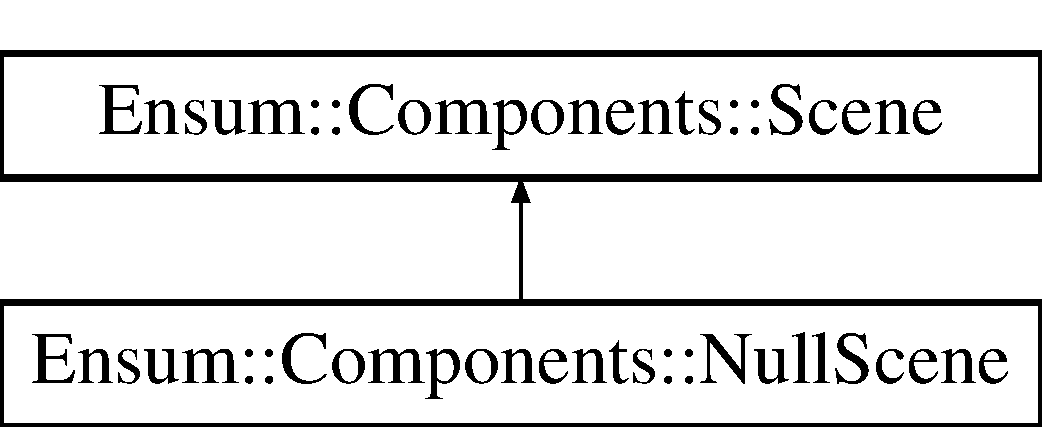
\includegraphics[height=2.000000cm]{class_ensum_1_1_components_1_1_scene}
\end{center}
\end{figure}
\subsection*{Public Member Functions}
\begin{DoxyCompactItemize}
\item 
virtual const \hyperlink{struct_ensum_1_1_components_1_1_entity}{Entity} \& \hyperlink{class_ensum_1_1_components_1_1_scene_ab614d491401edd9db3584d4e61ef6416}{Get\+Entity} () const \hypertarget{class_ensum_1_1_components_1_1_scene_ab614d491401edd9db3584d4e61ef6416}{}\label{class_ensum_1_1_components_1_1_scene_ab614d491401edd9db3584d4e61ef6416}

\begin{DoxyCompactList}\small\item\em Returns the scenes entity. \end{DoxyCompactList}\item 
virtual const void \hyperlink{class_ensum_1_1_components_1_1_scene_a4f12d73cbbd3e203bfc60eac07318985}{Frame} ()\hypertarget{class_ensum_1_1_components_1_1_scene_a4f12d73cbbd3e203bfc60eac07318985}{}\label{class_ensum_1_1_components_1_1_scene_a4f12d73cbbd3e203bfc60eac07318985}

\begin{DoxyCompactList}\small\item\em The frame function for the scene. \end{DoxyCompactList}\end{DoxyCompactItemize}
\subsection*{Protected Member Functions}
\begin{DoxyCompactItemize}
\item 
{\bfseries Scene} (\hyperlink{class_ensum_1_1_components_1_1_entity_manager}{Entity\+Manager} \&entity\+Manger, \hyperlink{class_ensum_1_1_input_1_1_input}{Input\+::\+Input} $\ast$input)\hypertarget{class_ensum_1_1_components_1_1_scene_aee190492d4435b67533941958ff81a8e}{}\label{class_ensum_1_1_components_1_1_scene_aee190492d4435b67533941958ff81a8e}

\end{DoxyCompactItemize}
\subsection*{Protected Attributes}
\begin{DoxyCompactItemize}
\item 
\hyperlink{struct_ensum_1_1_components_1_1_entity}{Entity} \hyperlink{class_ensum_1_1_components_1_1_scene_a8d36e81874a5b07e3edbd8720b8b289e}{\+\_\+entity}
\item 
\hyperlink{class_ensum_1_1_components_1_1_entity_manager}{Entity\+Manager} \& \hyperlink{class_ensum_1_1_components_1_1_scene_af7eb8e3279c5b6768f442ae05b44e75f}{\+\_\+entity\+Manager}
\item 
\hyperlink{class_ensum_1_1_input_1_1_input}{Input\+::\+Input} $\ast$ {\bfseries \+\_\+input}\hypertarget{class_ensum_1_1_components_1_1_scene_ab7ee39773379321c85d73984b03c5568}{}\label{class_ensum_1_1_components_1_1_scene_ab7ee39773379321c85d73984b03c5568}

\item 
std\+::vector$<$ \hyperlink{class_ensum_1_1_components_1_1_manager}{Manager} $\ast$ $>$ $\ast$ \hyperlink{class_ensum_1_1_components_1_1_scene_a9f7c53f74805c8bf7461f9ff2c818be7}{\+\_\+managers}
\begin{DoxyCompactList}\small\item\em Create new instance of all other managers here. \end{DoxyCompactList}\item 
\hyperlink{class_ensum_1_1_components_1_1_data_manager}{Data\+Manager} {\bfseries \+\_\+data}\hypertarget{class_ensum_1_1_components_1_1_scene_ae6357dc18aece3e778ce642f59f8195b}{}\label{class_ensum_1_1_components_1_1_scene_ae6357dc18aece3e778ce642f59f8195b}

\item 
\hyperlink{class_ensum_1_1_components_1_1_transform_manager}{Transform\+Manager} {\bfseries \+\_\+transform}\hypertarget{class_ensum_1_1_components_1_1_scene_a9f8a3149409a891d77b5554c154deb65}{}\label{class_ensum_1_1_components_1_1_scene_a9f8a3149409a891d77b5554c154deb65}

\item 
\hyperlink{class_ensum_1_1_components_1_1_camera_manager}{Camera\+Manager} {\bfseries \+\_\+camera}\hypertarget{class_ensum_1_1_components_1_1_scene_a9d4a91f7879f6392a6d95dfeea6608a2}{}\label{class_ensum_1_1_components_1_1_scene_a9d4a91f7879f6392a6d95dfeea6608a2}

\item 
\hyperlink{class_ensum_1_1_components_1_1_static_mesh_manager}{Static\+Mesh\+Manager} {\bfseries \+\_\+static\+Meshes}\hypertarget{class_ensum_1_1_components_1_1_scene_a790b65abe3f86eae4e082a4557fc07d8}{}\label{class_ensum_1_1_components_1_1_scene_a790b65abe3f86eae4e082a4557fc07d8}

\end{DoxyCompactItemize}


\subsection{Detailed Description}
The abstract scene class. 

A scene could be considered it\textquotesingle{}s own world or a state in a statemachine. 

\subsection{Member Data Documentation}
\index{Ensum\+::\+Components\+::\+Scene@{Ensum\+::\+Components\+::\+Scene}!\+\_\+entity@{\+\_\+entity}}
\index{\+\_\+entity@{\+\_\+entity}!Ensum\+::\+Components\+::\+Scene@{Ensum\+::\+Components\+::\+Scene}}
\subsubsection[{\texorpdfstring{\+\_\+entity}{_entity}}]{\setlength{\rightskip}{0pt plus 5cm}{\bf Entity} Ensum\+::\+Components\+::\+Scene\+::\+\_\+entity\hspace{0.3cm}{\ttfamily [protected]}}\hypertarget{class_ensum_1_1_components_1_1_scene_a8d36e81874a5b07e3edbd8720b8b289e}{}\label{class_ensum_1_1_components_1_1_scene_a8d36e81874a5b07e3edbd8720b8b289e}
The scenes own entity \index{Ensum\+::\+Components\+::\+Scene@{Ensum\+::\+Components\+::\+Scene}!\+\_\+entity\+Manager@{\+\_\+entity\+Manager}}
\index{\+\_\+entity\+Manager@{\+\_\+entity\+Manager}!Ensum\+::\+Components\+::\+Scene@{Ensum\+::\+Components\+::\+Scene}}
\subsubsection[{\texorpdfstring{\+\_\+entity\+Manager}{_entityManager}}]{\setlength{\rightskip}{0pt plus 5cm}{\bf Entity\+Manager}\& Ensum\+::\+Components\+::\+Scene\+::\+\_\+entity\+Manager\hspace{0.3cm}{\ttfamily [protected]}}\hypertarget{class_ensum_1_1_components_1_1_scene_af7eb8e3279c5b6768f442ae05b44e75f}{}\label{class_ensum_1_1_components_1_1_scene_af7eb8e3279c5b6768f442ae05b44e75f}
A reference to the entitymanager created in scenemanager \index{Ensum\+::\+Components\+::\+Scene@{Ensum\+::\+Components\+::\+Scene}!\+\_\+managers@{\+\_\+managers}}
\index{\+\_\+managers@{\+\_\+managers}!Ensum\+::\+Components\+::\+Scene@{Ensum\+::\+Components\+::\+Scene}}
\subsubsection[{\texorpdfstring{\+\_\+managers}{_managers}}]{\setlength{\rightskip}{0pt plus 5cm}std\+::vector$<${\bf Manager}$\ast$$>$$\ast$ Ensum\+::\+Components\+::\+Scene\+::\+\_\+managers\hspace{0.3cm}{\ttfamily [protected]}}\hypertarget{class_ensum_1_1_components_1_1_scene_a9f7c53f74805c8bf7461f9ff2c818be7}{}\label{class_ensum_1_1_components_1_1_scene_a9f7c53f74805c8bf7461f9ff2c818be7}


Create new instance of all other managers here. 

Every new manager needs to be initiated in the constructor and added to the managers vector. 

The documentation for this class was generated from the following file\+:\begin{DoxyCompactItemize}
\item 
C\+:/\+Users/peter/\+Source/\+Repos/\+E\+N\+S\+U\+M/\+Ensum/\+Includes/\+Ensum\+\_\+components/Scene.\+h\end{DoxyCompactItemize}

\hypertarget{struct_ensum_1_1_components_1_1_scene_manager_1_1_scene_data}{}\section{Ensum\+:\+:Components\+:\+:Scene\+Manager\+:\+:Scene\+Data Struct Reference}
\label{struct_ensum_1_1_components_1_1_scene_manager_1_1_scene_data}\index{Ensum\+::\+Components\+::\+Scene\+Manager\+::\+Scene\+Data@{Ensum\+::\+Components\+::\+Scene\+Manager\+::\+Scene\+Data}}
\subsection*{Public Attributes}
\begin{DoxyCompactItemize}
\item 
\hyperlink{struct_meta_data}{Meta\+Data} {\bfseries meta}\hypertarget{struct_ensum_1_1_components_1_1_scene_manager_1_1_scene_data_a86f40c9cb2aa13ae41ee7521dcf416cc}{}\label{struct_ensum_1_1_components_1_1_scene_manager_1_1_scene_data_a86f40c9cb2aa13ae41ee7521dcf416cc}

\item 
\hyperlink{struct_ensum_1_1_components_1_1_entity}{Entity} $\ast$ {\bfseries entity}\hypertarget{struct_ensum_1_1_components_1_1_scene_manager_1_1_scene_data_aff477aef5752b1b0f438ef0e986a9229}{}\label{struct_ensum_1_1_components_1_1_scene_manager_1_1_scene_data_aff477aef5752b1b0f438ef0e986a9229}

\item 
\hyperlink{class_ensum_1_1_components_1_1_scene}{Scene} $\ast$$\ast$ {\bfseries scene\+Ptr}\hypertarget{struct_ensum_1_1_components_1_1_scene_manager_1_1_scene_data_ac37964615c53887051adcc587fa9dab0}{}\label{struct_ensum_1_1_components_1_1_scene_manager_1_1_scene_data_ac37964615c53887051adcc587fa9dab0}

\item 
bool $\ast$ {\bfseries scene\+Update}\hypertarget{struct_ensum_1_1_components_1_1_scene_manager_1_1_scene_data_a7d4a9e3d7aed5dc8f338b4d4a312f875}{}\label{struct_ensum_1_1_components_1_1_scene_manager_1_1_scene_data_a7d4a9e3d7aed5dc8f338b4d4a312f875}

\end{DoxyCompactItemize}


The documentation for this struct was generated from the following file\+:\begin{DoxyCompactItemize}
\item 
Includes/\+Ensum\+\_\+components/Scene\+Manager.\+h\end{DoxyCompactItemize}

\hypertarget{class_ensum_1_1_components_1_1_scene_manager}{}\section{Ensum\+:\+:Components\+:\+:Scene\+Manager Class Reference}
\label{class_ensum_1_1_components_1_1_scene_manager}\index{Ensum\+::\+Components\+::\+Scene\+Manager@{Ensum\+::\+Components\+::\+Scene\+Manager}}


Manages all the scenes.  




{\ttfamily \#include $<$Scene\+Manager.\+h$>$}

Inheritance diagram for Ensum\+:\+:Components\+:\+:Scene\+Manager\+:\begin{figure}[H]
\begin{center}
\leavevmode
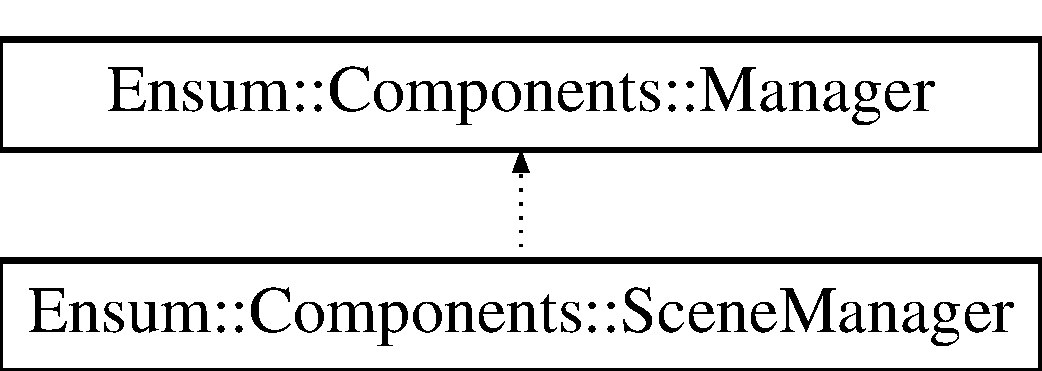
\includegraphics[height=2.000000cm]{class_ensum_1_1_components_1_1_scene_manager}
\end{center}
\end{figure}
\subsection*{Classes}
\begin{DoxyCompactItemize}
\item 
struct \hyperlink{struct_ensum_1_1_components_1_1_scene_manager_1_1_scene_data}{Scene\+Data}
\end{DoxyCompactItemize}
\subsection*{Public Member Functions}
\begin{DoxyCompactItemize}
\item 
const \hyperlink{struct_ensum_1_1_components_1_1_entity}{Entity} \& \hyperlink{class_ensum_1_1_components_1_1_scene_manager_a4a71bb9192da118a71f1b81ca49742cb}{Create\+Scene} (\hyperlink{class_ensum_1_1_components_1_1_scene}{Scene} $\ast$scene)\hypertarget{class_ensum_1_1_components_1_1_scene_manager_a4a71bb9192da118a71f1b81ca49742cb}{}\label{class_ensum_1_1_components_1_1_scene_manager_a4a71bb9192da118a71f1b81ca49742cb}

\begin{DoxyCompactList}\small\item\em Create the scene and return it\textquotesingle{}s entity. \end{DoxyCompactList}\item 
const void \hyperlink{class_ensum_1_1_components_1_1_scene_manager_ab970d3716b08c39b9b8c5484dea11595}{Remove\+Scene} (const \hyperlink{struct_ensum_1_1_components_1_1_entity}{Entity} \&scene\+Entity)\hypertarget{class_ensum_1_1_components_1_1_scene_manager_ab970d3716b08c39b9b8c5484dea11595}{}\label{class_ensum_1_1_components_1_1_scene_manager_ab970d3716b08c39b9b8c5484dea11595}

\begin{DoxyCompactList}\small\item\em Remove the scene component from the entity. \end{DoxyCompactList}\item 
const void \hyperlink{class_ensum_1_1_components_1_1_scene_manager_aea9f13488931b4448778e5563685428e}{Set\+Update} (const \hyperlink{struct_ensum_1_1_components_1_1_entity}{Entity} \&scene\+Entity, bool update)\hypertarget{class_ensum_1_1_components_1_1_scene_manager_aea9f13488931b4448778e5563685428e}{}\label{class_ensum_1_1_components_1_1_scene_manager_aea9f13488931b4448778e5563685428e}

\begin{DoxyCompactList}\small\item\em Specifies whether the scene should be updated each frame. \end{DoxyCompactList}\item 
const void \hyperlink{class_ensum_1_1_components_1_1_scene_manager_ad33a35aa27eeae297a4f16c610205d8a}{Frame} ()\hypertarget{class_ensum_1_1_components_1_1_scene_manager_ad33a35aa27eeae297a4f16c610205d8a}{}\label{class_ensum_1_1_components_1_1_scene_manager_ad33a35aa27eeae297a4f16c610205d8a}

\begin{DoxyCompactList}\small\item\em Do the framework for all active scenes. \end{DoxyCompactList}\item 
\hyperlink{class_ensum_1_1_components_1_1_entity_manager}{Entity\+Manager} \& \hyperlink{class_ensum_1_1_components_1_1_scene_manager_a7fdc5d47c5b8fe03807fe472b038a56f}{Get\+Entity\+Manager} ()\hypertarget{class_ensum_1_1_components_1_1_scene_manager_a7fdc5d47c5b8fe03807fe472b038a56f}{}\label{class_ensum_1_1_components_1_1_scene_manager_a7fdc5d47c5b8fe03807fe472b038a56f}

\begin{DoxyCompactList}\small\item\em Return a reference to the entity manager. \end{DoxyCompactList}\end{DoxyCompactItemize}
\subsection*{Private Member Functions}
\begin{DoxyCompactItemize}
\item 
const void \hyperlink{class_ensum_1_1_components_1_1_scene_manager_a383a468319c93280ce8ac0bbb920ab87}{\+\_\+\+Allocate} (uint32\+\_\+t size)
\begin{DoxyCompactList}\small\item\em Allocate more memory for scenedata. \end{DoxyCompactList}\item 
const void \hyperlink{class_ensum_1_1_components_1_1_scene_manager_a8102cfd9f4fed62a06e564dc016b6c46}{\+\_\+\+Destroy} (uint32\+\_\+t index)
\begin{DoxyCompactList}\small\item\em Delete an entry in the memory block. \end{DoxyCompactList}\end{DoxyCompactItemize}
\subsection*{Private Attributes}
\begin{DoxyCompactItemize}
\item 
\hyperlink{class_ensum_1_1_components_1_1_entity_manager}{Entity\+Manager} \hyperlink{class_ensum_1_1_components_1_1_scene_manager_a1be3bed380d7f6712e9c6c3bb71c048a}{\+\_\+ent\+Manager}\hypertarget{class_ensum_1_1_components_1_1_scene_manager_a1be3bed380d7f6712e9c6c3bb71c048a}{}\label{class_ensum_1_1_components_1_1_scene_manager_a1be3bed380d7f6712e9c6c3bb71c048a}

\begin{DoxyCompactList}\small\item\em Looks for destroyed entities and deletes them from the data block. \end{DoxyCompactList}\item 
\hyperlink{class_ensum_1_1_input_1_1_input}{Input\+::\+Input} $\ast$ {\bfseries \+\_\+input}\hypertarget{class_ensum_1_1_components_1_1_scene_manager_a997e4d367f66c9f80d27e027999f6802}{}\label{class_ensum_1_1_components_1_1_scene_manager_a997e4d367f66c9f80d27e027999f6802}

\item 
\hyperlink{struct_ensum_1_1_components_1_1_scene_manager_1_1_scene_data}{Scene\+Data} $\ast$ {\bfseries \+\_\+datap}\hypertarget{class_ensum_1_1_components_1_1_scene_manager_a249b282fedd2971d521e5a4a8922ceeb}{}\label{class_ensum_1_1_components_1_1_scene_manager_a249b282fedd2971d521e5a4a8922ceeb}

\end{DoxyCompactItemize}


\subsection{Detailed Description}
Manages all the scenes. 

\subsection{Member Function Documentation}
\index{Ensum\+::\+Components\+::\+Scene\+Manager@{Ensum\+::\+Components\+::\+Scene\+Manager}!\+\_\+\+Allocate@{\+\_\+\+Allocate}}
\index{\+\_\+\+Allocate@{\+\_\+\+Allocate}!Ensum\+::\+Components\+::\+Scene\+Manager@{Ensum\+::\+Components\+::\+Scene\+Manager}}
\subsubsection[{\texorpdfstring{\+\_\+\+Allocate(uint32\+\_\+t size)}{_Allocate(uint32_t size)}}]{\setlength{\rightskip}{0pt plus 5cm}const void Ensum\+::\+Components\+::\+Scene\+Manager\+::\+\_\+\+Allocate (
\begin{DoxyParamCaption}
\item[{uint32\+\_\+t}]{size}
\end{DoxyParamCaption}
)\hspace{0.3cm}{\ttfamily [private]}, {\ttfamily [virtual]}}\hypertarget{class_ensum_1_1_components_1_1_scene_manager_a383a468319c93280ce8ac0bbb920ab87}{}\label{class_ensum_1_1_components_1_1_scene_manager_a383a468319c93280ce8ac0bbb920ab87}


Allocate more memory for scenedata. 



Implements \hyperlink{class_ensum_1_1_components_1_1_manager_a1b593059210d09632c910a6abaae49c0}{Ensum\+::\+Components\+::\+Manager}.

\index{Ensum\+::\+Components\+::\+Scene\+Manager@{Ensum\+::\+Components\+::\+Scene\+Manager}!\+\_\+\+Destroy@{\+\_\+\+Destroy}}
\index{\+\_\+\+Destroy@{\+\_\+\+Destroy}!Ensum\+::\+Components\+::\+Scene\+Manager@{Ensum\+::\+Components\+::\+Scene\+Manager}}
\subsubsection[{\texorpdfstring{\+\_\+\+Destroy(uint32\+\_\+t index)}{_Destroy(uint32_t index)}}]{\setlength{\rightskip}{0pt plus 5cm}const void Ensum\+::\+Components\+::\+Scene\+Manager\+::\+\_\+\+Destroy (
\begin{DoxyParamCaption}
\item[{uint32\+\_\+t}]{index}
\end{DoxyParamCaption}
)\hspace{0.3cm}{\ttfamily [private]}, {\ttfamily [virtual]}}\hypertarget{class_ensum_1_1_components_1_1_scene_manager_a8102cfd9f4fed62a06e564dc016b6c46}{}\label{class_ensum_1_1_components_1_1_scene_manager_a8102cfd9f4fed62a06e564dc016b6c46}


Delete an entry in the memory block. 

The deleted entry is replaced by the last in the block. 

Implements \hyperlink{class_ensum_1_1_components_1_1_manager_a5ba85395802e942ed8904ca18951e6b0}{Ensum\+::\+Components\+::\+Manager}.



The documentation for this class was generated from the following file\+:\begin{DoxyCompactItemize}
\item 
C\+:/\+Users/peter/\+Source/\+Repos/\+E\+N\+S\+U\+M/\+Ensum/\+Includes/\+Ensum\+\_\+components/Scene\+Manager.\+h\end{DoxyCompactItemize}

\hypertarget{struct_ensum_1_1_file_handler_1_1ini_1_1_section}{}\section{Ensum\+:\+:File\+Handler\+:\+:ini\+:\+:Section Struct Reference}
\label{struct_ensum_1_1_file_handler_1_1ini_1_1_section}\index{Ensum\+::\+File\+Handler\+::ini\+::\+Section@{Ensum\+::\+File\+Handler\+::ini\+::\+Section}}
\subsection*{Public Member Functions}
\begin{DoxyCompactItemize}
\item 
{\bfseries Section} (const \hyperlink{class_ensum_1_1string}{string} \&sname)\hypertarget{struct_ensum_1_1_file_handler_1_1ini_1_1_section_aece352bd19575c13a3359ee2a16f375d}{}\label{struct_ensum_1_1_file_handler_1_1ini_1_1_section_aece352bd19575c13a3359ee2a16f375d}

\end{DoxyCompactItemize}
\subsection*{Public Attributes}
\begin{DoxyCompactItemize}
\item 
\hyperlink{class_ensum_1_1string}{string} {\bfseries name}\hypertarget{struct_ensum_1_1_file_handler_1_1ini_1_1_section_aaef5921ebec35dfe6b7ac00cde2e71a6}{}\label{struct_ensum_1_1_file_handler_1_1ini_1_1_section_aaef5921ebec35dfe6b7ac00cde2e71a6}

\item 
std\+::vector$<$ \hyperlink{struct_ensum_1_1_file_handler_1_1ini_1_1_key}{Key} $>$ {\bfseries keys}\hypertarget{struct_ensum_1_1_file_handler_1_1ini_1_1_section_a4ef77125d407902a380c30d3f0f120da}{}\label{struct_ensum_1_1_file_handler_1_1ini_1_1_section_a4ef77125d407902a380c30d3f0f120da}

\end{DoxyCompactItemize}


The documentation for this struct was generated from the following file\+:\begin{DoxyCompactItemize}
\item 
Includes/\+Ensum\+\_\+filehandler/Ini.\+h\end{DoxyCompactItemize}

\hypertarget{class_ensum_1_1_components_1_1_static_mesh_manager}{}\section{Ensum\+:\+:Components\+:\+:Static\+Mesh\+Manager Class Reference}
\label{class_ensum_1_1_components_1_1_static_mesh_manager}\index{Ensum\+::\+Components\+::\+Static\+Mesh\+Manager@{Ensum\+::\+Components\+::\+Static\+Mesh\+Manager}}


Handles meshes for entities.  




{\ttfamily \#include $<$Static\+Mesh\+Manager.\+h$>$}

Inheritance diagram for Ensum\+:\+:Components\+:\+:Static\+Mesh\+Manager\+:\begin{figure}[H]
\begin{center}
\leavevmode
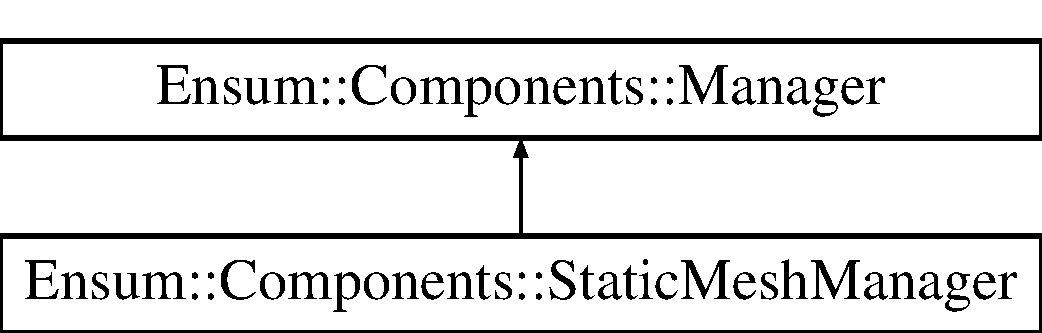
\includegraphics[height=2.000000cm]{class_ensum_1_1_components_1_1_static_mesh_manager}
\end{center}
\end{figure}
\subsection*{Classes}
\begin{DoxyCompactItemize}
\item 
struct \hyperlink{struct_ensum_1_1_components_1_1_static_mesh_manager_1_1_mesh_component}{Mesh\+Component}
\begin{DoxyCompactList}\small\item\em The managers data struct. \end{DoxyCompactList}\end{DoxyCompactItemize}
\subsection*{Public Member Functions}
\begin{DoxyCompactItemize}
\item 
{\bfseries Static\+Mesh\+Manager} (\hyperlink{class_ensum_1_1_components_1_1_entity_manager}{Entity\+Manager} \&ent\+Manager)\hypertarget{class_ensum_1_1_components_1_1_static_mesh_manager_a36c1b89e93c9ca37855b709b9e5c8268}{}\label{class_ensum_1_1_components_1_1_static_mesh_manager_a36c1b89e93c9ca37855b709b9e5c8268}

\item 
const void \hyperlink{class_ensum_1_1_components_1_1_static_mesh_manager_a693d1787a0e9e52118e26b66d6d4d01e}{Create\+Static\+Mesh} (const \hyperlink{struct_ensum_1_1_components_1_1_entity}{Entity} \&entity, const char $\ast$path)\hypertarget{class_ensum_1_1_components_1_1_static_mesh_manager_a693d1787a0e9e52118e26b66d6d4d01e}{}\label{class_ensum_1_1_components_1_1_static_mesh_manager_a693d1787a0e9e52118e26b66d6d4d01e}

\begin{DoxyCompactList}\small\item\em Create a static mesh for the entity. \end{DoxyCompactList}\end{DoxyCompactItemize}
\subsection*{Private Member Functions}
\begin{DoxyCompactItemize}
\item 
const void \hyperlink{class_ensum_1_1_components_1_1_static_mesh_manager_a470c7fb98f91c55b803ef8d2dd7a4803}{\+\_\+\+Allocate} (uint32\+\_\+t size)
\begin{DoxyCompactList}\small\item\em Allocate more memory. \end{DoxyCompactList}\item 
const void \hyperlink{class_ensum_1_1_components_1_1_static_mesh_manager_a3d7684a00092ff8d467425a9f1ba7e5c}{\+\_\+\+Destroy} (uint32\+\_\+t index)
\begin{DoxyCompactList}\small\item\em Delete an entry in the memory block. \end{DoxyCompactList}\end{DoxyCompactItemize}
\subsection*{Private Attributes}
\begin{DoxyCompactItemize}
\item 
std\+::unordered\+\_\+map$<$ uint32\+\_\+t, \hyperlink{struct_ensum_1_1_file_handler_1_1_mesh_data}{File\+Handler\+::\+Mesh\+Data} $>$ $\ast$ {\bfseries \+\_\+loaded\+Meshes}\hypertarget{class_ensum_1_1_components_1_1_static_mesh_manager_a79e92dda1ad0d4aa9fd87ea808258add}{}\label{class_ensum_1_1_components_1_1_static_mesh_manager_a79e92dda1ad0d4aa9fd87ea808258add}

\item 
\hyperlink{struct_ensum_1_1_components_1_1_static_mesh_manager_1_1_mesh_component}{Mesh\+Component} $\ast$ \hyperlink{class_ensum_1_1_components_1_1_static_mesh_manager_af47fea699c4d1241d82ca9374a7a48ad}{\+\_\+datap}
\end{DoxyCompactItemize}
\subsection*{Additional Inherited Members}


\subsection{Detailed Description}
Handles meshes for entities. 

Static/\+Non-\/\+Animated 

\subsection{Member Function Documentation}
\index{Ensum\+::\+Components\+::\+Static\+Mesh\+Manager@{Ensum\+::\+Components\+::\+Static\+Mesh\+Manager}!\+\_\+\+Allocate@{\+\_\+\+Allocate}}
\index{\+\_\+\+Allocate@{\+\_\+\+Allocate}!Ensum\+::\+Components\+::\+Static\+Mesh\+Manager@{Ensum\+::\+Components\+::\+Static\+Mesh\+Manager}}
\subsubsection[{\texorpdfstring{\+\_\+\+Allocate(uint32\+\_\+t size)}{_Allocate(uint32_t size)}}]{\setlength{\rightskip}{0pt plus 5cm}const void Ensum\+::\+Components\+::\+Static\+Mesh\+Manager\+::\+\_\+\+Allocate (
\begin{DoxyParamCaption}
\item[{uint32\+\_\+t}]{size}
\end{DoxyParamCaption}
)\hspace{0.3cm}{\ttfamily [private]}, {\ttfamily [virtual]}}\hypertarget{class_ensum_1_1_components_1_1_static_mesh_manager_a470c7fb98f91c55b803ef8d2dd7a4803}{}\label{class_ensum_1_1_components_1_1_static_mesh_manager_a470c7fb98f91c55b803ef8d2dd7a4803}


Allocate more memory. 



Implements \hyperlink{class_ensum_1_1_components_1_1_manager_a1b593059210d09632c910a6abaae49c0}{Ensum\+::\+Components\+::\+Manager}.

\index{Ensum\+::\+Components\+::\+Static\+Mesh\+Manager@{Ensum\+::\+Components\+::\+Static\+Mesh\+Manager}!\+\_\+\+Destroy@{\+\_\+\+Destroy}}
\index{\+\_\+\+Destroy@{\+\_\+\+Destroy}!Ensum\+::\+Components\+::\+Static\+Mesh\+Manager@{Ensum\+::\+Components\+::\+Static\+Mesh\+Manager}}
\subsubsection[{\texorpdfstring{\+\_\+\+Destroy(uint32\+\_\+t index)}{_Destroy(uint32_t index)}}]{\setlength{\rightskip}{0pt plus 5cm}const void Ensum\+::\+Components\+::\+Static\+Mesh\+Manager\+::\+\_\+\+Destroy (
\begin{DoxyParamCaption}
\item[{uint32\+\_\+t}]{index}
\end{DoxyParamCaption}
)\hspace{0.3cm}{\ttfamily [private]}, {\ttfamily [virtual]}}\hypertarget{class_ensum_1_1_components_1_1_static_mesh_manager_a3d7684a00092ff8d467425a9f1ba7e5c}{}\label{class_ensum_1_1_components_1_1_static_mesh_manager_a3d7684a00092ff8d467425a9f1ba7e5c}


Delete an entry in the memory block. 

The deleted entry is replaced by the last in the block. 

Implements \hyperlink{class_ensum_1_1_components_1_1_manager_a5ba85395802e942ed8904ca18951e6b0}{Ensum\+::\+Components\+::\+Manager}.



\subsection{Member Data Documentation}
\index{Ensum\+::\+Components\+::\+Static\+Mesh\+Manager@{Ensum\+::\+Components\+::\+Static\+Mesh\+Manager}!\+\_\+datap@{\+\_\+datap}}
\index{\+\_\+datap@{\+\_\+datap}!Ensum\+::\+Components\+::\+Static\+Mesh\+Manager@{Ensum\+::\+Components\+::\+Static\+Mesh\+Manager}}
\subsubsection[{\texorpdfstring{\+\_\+datap}{_datap}}]{\setlength{\rightskip}{0pt plus 5cm}{\bf Mesh\+Component}$\ast$ Ensum\+::\+Components\+::\+Static\+Mesh\+Manager\+::\+\_\+datap\hspace{0.3cm}{\ttfamily [private]}}\hypertarget{class_ensum_1_1_components_1_1_static_mesh_manager_af47fea699c4d1241d82ca9374a7a48ad}{}\label{class_ensum_1_1_components_1_1_static_mesh_manager_af47fea699c4d1241d82ca9374a7a48ad}
A reference pointer to avoid having to cast the basic datapointer all the time. 

The documentation for this class was generated from the following file\+:\begin{DoxyCompactItemize}
\item 
C\+:/\+Users/peter/\+Source/\+Repos/\+E\+N\+S\+U\+M/\+Ensum/\+Includes/\+Ensum\+\_\+components/Static\+Mesh\+Manager.\+h\end{DoxyCompactItemize}

\hypertarget{class_ensum_1_1string}{}\section{Ensum\+:\+:string Class Reference}
\label{class_ensum_1_1string}\index{Ensum\+::string@{Ensum\+::string}}


A wrapper class for std\+::string.  




{\ttfamily \#include $<$ensumstring.\+h$>$}

\subsection*{Public Member Functions}
\begin{DoxyCompactItemize}
\item 
{\bfseries string} (const char $\ast$str)\hypertarget{class_ensum_1_1string_a1efde732b942cf5b4a9aeff02836c7f4}{}\label{class_ensum_1_1string_a1efde732b942cf5b4a9aeff02836c7f4}

\item 
{\bfseries string} (const \hyperlink{class_ensum_1_1string}{string} \&other)\hypertarget{class_ensum_1_1string_a941a6aeb4f7e6f8a61a375a19ada9e36}{}\label{class_ensum_1_1string_a941a6aeb4f7e6f8a61a375a19ada9e36}

\item 
{\bfseries string} (const long \&other)\hypertarget{class_ensum_1_1string_ab94e9717ef713acd5981ad9d2c9d0a5e}{}\label{class_ensum_1_1string_ab94e9717ef713acd5981ad9d2c9d0a5e}

\item 
{\bfseries string} (const double \&other)\hypertarget{class_ensum_1_1string_ad2d7d12b303783eb4ecc32a389e1c42b}{}\label{class_ensum_1_1string_ad2d7d12b303783eb4ecc32a389e1c42b}

\item 
{\bfseries string} (const bool \&other)\hypertarget{class_ensum_1_1string_a82ccf9bec24664a575b8e9c70cbd7d99}{}\label{class_ensum_1_1string_a82ccf9bec24664a575b8e9c70cbd7d99}

\item 
\hyperlink{class_ensum_1_1string}{string} \hyperlink{class_ensum_1_1string_a13098a5e0f0fd18baeffa5bc8b35494d}{operator+} (const \hyperlink{class_ensum_1_1string}{string} \&str) const 
\item 
\hyperlink{class_ensum_1_1string}{string} \hyperlink{class_ensum_1_1string_aa9f884ae697a27d375d6dc71fd5a1602}{operator+} (const char $\ast$str) const 
\item 
\hyperlink{class_ensum_1_1string_ae1473c4afee1fb83de48490a72f8266b}{operator const char $\ast$} () const \hypertarget{class_ensum_1_1string_ae1473c4afee1fb83de48490a72f8266b}{}\label{class_ensum_1_1string_ae1473c4afee1fb83de48490a72f8266b}

\begin{DoxyCompactList}\small\item\em convertion operator to char$\ast$. \end{DoxyCompactList}\item 
\hyperlink{class_ensum_1_1string_a6fa9ce4490f285575c2d06a1e64a93a7}{operator const void $\ast$} () const \hypertarget{class_ensum_1_1string_a6fa9ce4490f285575c2d06a1e64a93a7}{}\label{class_ensum_1_1string_a6fa9ce4490f285575c2d06a1e64a93a7}

\begin{DoxyCompactList}\small\item\em convertion operator to void$\ast$. \end{DoxyCompactList}\item 
\hyperlink{class_ensum_1_1string}{string} \& \hyperlink{class_ensum_1_1string_ae48b8f643d8cd3ff379a51484ea738d1}{operator=} (const char $\ast$str)\hypertarget{class_ensum_1_1string_ae48b8f643d8cd3ff379a51484ea738d1}{}\label{class_ensum_1_1string_ae48b8f643d8cd3ff379a51484ea738d1}

\begin{DoxyCompactList}\small\item\em = operator char. \end{DoxyCompactList}\item 
\hyperlink{class_ensum_1_1string}{string} \& \hyperlink{class_ensum_1_1string_a7903e871b1cf12584d746536241fa7ea}{operator=} (const \hyperlink{class_ensum_1_1string}{string} \&other)\hypertarget{class_ensum_1_1string_a7903e871b1cf12584d746536241fa7ea}{}\label{class_ensum_1_1string_a7903e871b1cf12584d746536241fa7ea}

\begin{DoxyCompactList}\small\item\em = operator string. \end{DoxyCompactList}\item 
const bool \hyperlink{class_ensum_1_1string_a6b5ab08eb5ef197bedb9e55e2eca0754}{operator==} (const char $\ast$str)\hypertarget{class_ensum_1_1string_a6b5ab08eb5ef197bedb9e55e2eca0754}{}\label{class_ensum_1_1string_a6b5ab08eb5ef197bedb9e55e2eca0754}

\begin{DoxyCompactList}\small\item\em == operator char. \end{DoxyCompactList}\item 
const bool \hyperlink{class_ensum_1_1string_a6429683caad1908c30cb77b4aa00ff4f}{operator==} (const \hyperlink{class_ensum_1_1string}{string} \&other)\hypertarget{class_ensum_1_1string_a6429683caad1908c30cb77b4aa00ff4f}{}\label{class_ensum_1_1string_a6429683caad1908c30cb77b4aa00ff4f}

\begin{DoxyCompactList}\small\item\em == operator string. \end{DoxyCompactList}\item 
const char $\ast$ \hyperlink{class_ensum_1_1string_a2d667ea4adbf4f9cd08011972176aacb}{c\+\_\+str} () const \hypertarget{class_ensum_1_1string_a2d667ea4adbf4f9cd08011972176aacb}{}\label{class_ensum_1_1string_a2d667ea4adbf4f9cd08011972176aacb}

\begin{DoxyCompactList}\small\item\em returns const char$\ast$. \end{DoxyCompactList}\item 
const void \hyperlink{class_ensum_1_1string_ad183e0697bed62d8e5639d17a5288a15}{transform} ()\hypertarget{class_ensum_1_1string_ad183e0697bed62d8e5639d17a5288a15}{}\label{class_ensum_1_1string_ad183e0697bed62d8e5639d17a5288a15}

\begin{DoxyCompactList}\small\item\em transforms all letters in string to lowercase. \end{DoxyCompactList}\item 
const void \hyperlink{class_ensum_1_1string_a27c098c250b2df7ed3fa935e0d318fe2}{clear} ()\hypertarget{class_ensum_1_1string_a27c098c250b2df7ed3fa935e0d318fe2}{}\label{class_ensum_1_1string_a27c098c250b2df7ed3fa935e0d318fe2}

\begin{DoxyCompactList}\small\item\em clears the string. \end{DoxyCompactList}\item 
const void \hyperlink{class_ensum_1_1string_af373cc0f29c09f8df78e3b96d279b609}{push\+\_\+back} (const char str)\hypertarget{class_ensum_1_1string_af373cc0f29c09f8df78e3b96d279b609}{}\label{class_ensum_1_1string_af373cc0f29c09f8df78e3b96d279b609}

\begin{DoxyCompactList}\small\item\em Adds char to end of string. \end{DoxyCompactList}\item 
const uint32\+\_\+t \hyperlink{class_ensum_1_1string_ac3c5ca17258824b74dc8da3d5b7602cd}{size} () const \hypertarget{class_ensum_1_1string_ac3c5ca17258824b74dc8da3d5b7602cd}{}\label{class_ensum_1_1string_ac3c5ca17258824b74dc8da3d5b7602cd}

\begin{DoxyCompactList}\small\item\em Returns the size of the string. \end{DoxyCompactList}\item 
const void \hyperlink{class_ensum_1_1string_a2cb9f50ce1653a174433276cb1373fd6}{Resize} (uint32\+\_\+t \hyperlink{class_ensum_1_1string_ac3c5ca17258824b74dc8da3d5b7602cd}{size})\hypertarget{class_ensum_1_1string_a2cb9f50ce1653a174433276cb1373fd6}{}\label{class_ensum_1_1string_a2cb9f50ce1653a174433276cb1373fd6}

\begin{DoxyCompactList}\small\item\em Resize the string. \end{DoxyCompactList}\item 
const uint32\+\_\+t \hyperlink{class_ensum_1_1string_ac7c2bfe9a65ef8c2c850cdc80501ee34}{Get\+Hash} () const \hypertarget{class_ensum_1_1string_ac7c2bfe9a65ef8c2c850cdc80501ee34}{}\label{class_ensum_1_1string_ac7c2bfe9a65ef8c2c850cdc80501ee34}

\begin{DoxyCompactList}\small\item\em Returns a hash of the string. \end{DoxyCompactList}\end{DoxyCompactItemize}
\subsection*{Private Attributes}
\begin{DoxyCompactItemize}
\item 
std\+::string $\ast$ {\bfseries \+\_\+string}\hypertarget{class_ensum_1_1string_aab7e7b28d0303d683f579b84754e761f}{}\label{class_ensum_1_1string_aab7e7b28d0303d683f579b84754e761f}

\item 
std\+::hash$<$ std\+::string $>$ {\bfseries hash}\hypertarget{class_ensum_1_1string_ac09465ae80a330532deb00843bf74f37}{}\label{class_ensum_1_1string_ac09465ae80a330532deb00843bf74f37}

\end{DoxyCompactItemize}


\subsection{Detailed Description}
A wrapper class for std\+::string. 

\subsection{Member Function Documentation}
\index{Ensum\+::string@{Ensum\+::string}!operator+@{operator+}}
\index{operator+@{operator+}!Ensum\+::string@{Ensum\+::string}}
\subsubsection[{\texorpdfstring{operator+(const string \&str) const }{operator+(const string &str) const }}]{\setlength{\rightskip}{0pt plus 5cm}{\bf string} Ensum\+::string\+::operator+ (
\begin{DoxyParamCaption}
\item[{const {\bf string} \&}]{str}
\end{DoxyParamCaption}
) const\hspace{0.3cm}{\ttfamily [inline]}}\hypertarget{class_ensum_1_1string_a13098a5e0f0fd18baeffa5bc8b35494d}{}\label{class_ensum_1_1string_a13098a5e0f0fd18baeffa5bc8b35494d}

\begin{DoxyItemize}
\item operator between strings. 
\end{DoxyItemize}\index{Ensum\+::string@{Ensum\+::string}!operator+@{operator+}}
\index{operator+@{operator+}!Ensum\+::string@{Ensum\+::string}}
\subsubsection[{\texorpdfstring{operator+(const char $\ast$str) const }{operator+(const char *str) const }}]{\setlength{\rightskip}{0pt plus 5cm}{\bf string} Ensum\+::string\+::operator+ (
\begin{DoxyParamCaption}
\item[{const char $\ast$}]{str}
\end{DoxyParamCaption}
) const\hspace{0.3cm}{\ttfamily [inline]}}\hypertarget{class_ensum_1_1string_aa9f884ae697a27d375d6dc71fd5a1602}{}\label{class_ensum_1_1string_aa9f884ae697a27d375d6dc71fd5a1602}

\begin{DoxyItemize}
\item operator string and char. 
\end{DoxyItemize}

The documentation for this class was generated from the following file\+:\begin{DoxyCompactItemize}
\item 
C\+:/\+Users/peter/\+Source/\+Repos/\+E\+N\+S\+U\+M/\+Ensum/\+Includes/ensumstring.\+h\end{DoxyCompactItemize}

\hypertarget{struct_ensum_1_1_graphics_1_1_structured_buffer}{}\section{Ensum\+:\+:Graphics\+:\+:Structured\+Buffer Struct Reference}
\label{struct_ensum_1_1_graphics_1_1_structured_buffer}\index{Ensum\+::\+Graphics\+::\+Structured\+Buffer@{Ensum\+::\+Graphics\+::\+Structured\+Buffer}}
\subsection*{Public Attributes}
\begin{DoxyCompactItemize}
\item 
I\+D3\+D11\+Buffer $\ast$ {\bfseries Buffer} = nullptr\hypertarget{struct_ensum_1_1_graphics_1_1_structured_buffer_a71cd7a627a1d3c6dd9406d6902c6bcc1}{}\label{struct_ensum_1_1_graphics_1_1_structured_buffer_a71cd7a627a1d3c6dd9406d6902c6bcc1}

\item 
I\+D3\+D11\+Shader\+Resource\+View $\ast$ {\bfseries S\+RV} = nullptr\hypertarget{struct_ensum_1_1_graphics_1_1_structured_buffer_a7f169a11451ed8783f93e08921cdf141}{}\label{struct_ensum_1_1_graphics_1_1_structured_buffer_a7f169a11451ed8783f93e08921cdf141}

\item 
I\+D3\+D11\+Unordered\+Access\+View $\ast$ {\bfseries U\+AV} = nullptr\hypertarget{struct_ensum_1_1_graphics_1_1_structured_buffer_accc2db7ce60d7d51832c3da3225bce52}{}\label{struct_ensum_1_1_graphics_1_1_structured_buffer_accc2db7ce60d7d51832c3da3225bce52}

\item 
unsigned {\bfseries Stride} = 0\hypertarget{struct_ensum_1_1_graphics_1_1_structured_buffer_a006c6f374dd1e046a97c444cf182ff4d}{}\label{struct_ensum_1_1_graphics_1_1_structured_buffer_a006c6f374dd1e046a97c444cf182ff4d}

\item 
unsigned {\bfseries Element\+Count} = 0\hypertarget{struct_ensum_1_1_graphics_1_1_structured_buffer_a3a508d28e2eeb7ef69cc467080b22807}{}\label{struct_ensum_1_1_graphics_1_1_structured_buffer_a3a508d28e2eeb7ef69cc467080b22807}

\end{DoxyCompactItemize}


The documentation for this struct was generated from the following file\+:\begin{DoxyCompactItemize}
\item 
C\+:/\+Users/peter/\+Source/\+Repos/\+E\+N\+S\+U\+M/\+Ensum/\+Includes/\+Ensum\+\_\+graphics/Direct3\+D11.\+h\end{DoxyCompactItemize}

\hypertarget{struct_ensum_1_1_file_handler_1_1_sub_mesh}{}\section{Ensum\+:\+:File\+Handler\+:\+:Sub\+Mesh Struct Reference}
\label{struct_ensum_1_1_file_handler_1_1_sub_mesh}\index{Ensum\+::\+File\+Handler\+::\+Sub\+Mesh@{Ensum\+::\+File\+Handler\+::\+Sub\+Mesh}}
\subsection*{Public Attributes}
\begin{DoxyCompactItemize}
\item 
char {\bfseries name} \mbox{[}100\mbox{]}\hypertarget{struct_ensum_1_1_file_handler_1_1_sub_mesh_abc000d2bb4ab4e284a3f3e3622e10293}{}\label{struct_ensum_1_1_file_handler_1_1_sub_mesh_abc000d2bb4ab4e284a3f3e3622e10293}

\item 
uint64\+\_\+t {\bfseries face\+Start}\hypertarget{struct_ensum_1_1_file_handler_1_1_sub_mesh_a43071b4ae61d7dbae72387a4c310e35d}{}\label{struct_ensum_1_1_file_handler_1_1_sub_mesh_a43071b4ae61d7dbae72387a4c310e35d}

\item 
uint64\+\_\+t {\bfseries face\+Count}\hypertarget{struct_ensum_1_1_file_handler_1_1_sub_mesh_a5e291ad042dfd49d3c4d7ea478b5065c}{}\label{struct_ensum_1_1_file_handler_1_1_sub_mesh_a5e291ad042dfd49d3c4d7ea478b5065c}

\end{DoxyCompactItemize}


The documentation for this struct was generated from the following file\+:\begin{DoxyCompactItemize}
\item 
C\+:/\+Users/peter/\+Source/\+Repos/\+E\+N\+S\+U\+M/\+Ensum/\+Includes/\+Ensum\+\_\+filehandler/Mesh.\+h\end{DoxyCompactItemize}

\hypertarget{struct_ensum_1_1_file_handler_1_1_tex_coord}{}\section{Ensum\+:\+:File\+Handler\+:\+:Tex\+Coord Struct Reference}
\label{struct_ensum_1_1_file_handler_1_1_tex_coord}\index{Ensum\+::\+File\+Handler\+::\+Tex\+Coord@{Ensum\+::\+File\+Handler\+::\+Tex\+Coord}}
\subsection*{Public Member Functions}
\begin{DoxyCompactItemize}
\item 
{\bfseries Tex\+Coord} (float u, float v, float w)\hypertarget{struct_ensum_1_1_file_handler_1_1_tex_coord_ade68c6d8e086d712bc8ec69d243bb3af}{}\label{struct_ensum_1_1_file_handler_1_1_tex_coord_ade68c6d8e086d712bc8ec69d243bb3af}

\end{DoxyCompactItemize}
\subsection*{Public Attributes}
\begin{DoxyCompactItemize}
\item 
float {\bfseries u}\hypertarget{struct_ensum_1_1_file_handler_1_1_tex_coord_a91c1c65798ca8268251f86a419434a37}{}\label{struct_ensum_1_1_file_handler_1_1_tex_coord_a91c1c65798ca8268251f86a419434a37}

\item 
float {\bfseries v}\hypertarget{struct_ensum_1_1_file_handler_1_1_tex_coord_a2a2884161c9b630989c48bfae943dd1e}{}\label{struct_ensum_1_1_file_handler_1_1_tex_coord_a2a2884161c9b630989c48bfae943dd1e}

\item 
float {\bfseries w}\hypertarget{struct_ensum_1_1_file_handler_1_1_tex_coord_aef4ff1dfc5871d77aeb58cb62bbc503b}{}\label{struct_ensum_1_1_file_handler_1_1_tex_coord_aef4ff1dfc5871d77aeb58cb62bbc503b}

\end{DoxyCompactItemize}


The documentation for this struct was generated from the following file\+:\begin{DoxyCompactItemize}
\item 
C\+:/\+Users/peter/\+Source/\+Repos/\+E\+N\+S\+U\+M/\+Ensum/\+Includes/\+Ensum\+\_\+filehandler/Mesh.\+h\end{DoxyCompactItemize}

\hypertarget{class_ensum_1_1_core_1_1_timer}{}\section{Ensum\+:\+:Core\+:\+:Timer Class Reference}
\label{class_ensum_1_1_core_1_1_timer}\index{Ensum\+::\+Core\+::\+Timer@{Ensum\+::\+Core\+::\+Timer}}


Keeps track of time.  




{\ttfamily \#include $<$Timer.\+h$>$}

\subsection*{Public Member Functions}
\begin{DoxyCompactItemize}
\item 
{\bfseries Timer} (bool start\+Immediately=false)\hypertarget{class_ensum_1_1_core_1_1_timer_a00fb09cc574dbebe502b40d1d627c85b}{}\label{class_ensum_1_1_core_1_1_timer_a00fb09cc574dbebe502b40d1d627c85b}

\item 
const void \hyperlink{class_ensum_1_1_core_1_1_timer_ae34e21c17fe8325daf806f2f30980fab}{Reset} (bool start\+Immediately=false)
\begin{DoxyCompactList}\small\item\em Reset all the timer values. \end{DoxyCompactList}\item 
const void \hyperlink{class_ensum_1_1_core_1_1_timer_a3f8cd57aade8eb858d68ba376053df25}{Start} ()\hypertarget{class_ensum_1_1_core_1_1_timer_a3f8cd57aade8eb858d68ba376053df25}{}\label{class_ensum_1_1_core_1_1_timer_a3f8cd57aade8eb858d68ba376053df25}

\begin{DoxyCompactList}\small\item\em Start the timer. \end{DoxyCompactList}\item 
const float \hyperlink{class_ensum_1_1_core_1_1_timer_ae6a7f78e18573adc4378485519bc2daf}{Get\+Total\+Time\+And\+Stop} ()\hypertarget{class_ensum_1_1_core_1_1_timer_ae6a7f78e18573adc4378485519bc2daf}{}\label{class_ensum_1_1_core_1_1_timer_ae6a7f78e18573adc4378485519bc2daf}

\begin{DoxyCompactList}\small\item\em Returns the timers total runtime, then stops the timer. \end{DoxyCompactList}\item 
const void \hyperlink{class_ensum_1_1_core_1_1_timer_a0b65dc7246e0ac5498ac3f2ede1f2c29}{Stop} ()\hypertarget{class_ensum_1_1_core_1_1_timer_a0b65dc7246e0ac5498ac3f2ede1f2c29}{}\label{class_ensum_1_1_core_1_1_timer_a0b65dc7246e0ac5498ac3f2ede1f2c29}

\begin{DoxyCompactList}\small\item\em Stops the timer. \end{DoxyCompactList}\item 
const float \hyperlink{class_ensum_1_1_core_1_1_timer_a41ef243e3c8538b48e50096f1bfe8ad3}{Total\+Time} ()\hypertarget{class_ensum_1_1_core_1_1_timer_a41ef243e3c8538b48e50096f1bfe8ad3}{}\label{class_ensum_1_1_core_1_1_timer_a41ef243e3c8538b48e50096f1bfe8ad3}

\begin{DoxyCompactList}\small\item\em Returns the timers total runtime. \end{DoxyCompactList}\item 
const float \hyperlink{class_ensum_1_1_core_1_1_timer_ad51253e9d84426e84728ec47c9532654}{Delta} ()\hypertarget{class_ensum_1_1_core_1_1_timer_ad51253e9d84426e84728ec47c9532654}{}\label{class_ensum_1_1_core_1_1_timer_ad51253e9d84426e84728ec47c9532654}

\begin{DoxyCompactList}\small\item\em Returns the time between last frame and this frame (delta time). \end{DoxyCompactList}\item 
const void \hyperlink{class_ensum_1_1_core_1_1_timer_a72e9509a79aad7d8ea103492c9c8124d}{Tick} ()
\begin{DoxyCompactList}\small\item\em The tick of the timer. \end{DoxyCompactList}\end{DoxyCompactItemize}
\subsection*{Private Attributes}
\begin{DoxyCompactItemize}
\item 
clock\+\_\+t {\bfseries \+\_\+start\+Time}\hypertarget{class_ensum_1_1_core_1_1_timer_aab6887cc2a2f30ce555deff5bc17696e}{}\label{class_ensum_1_1_core_1_1_timer_aab6887cc2a2f30ce555deff5bc17696e}

\item 
clock\+\_\+t {\bfseries \+\_\+prev\+Time}\hypertarget{class_ensum_1_1_core_1_1_timer_a2ba284502edc94522fe618279bb16529}{}\label{class_ensum_1_1_core_1_1_timer_a2ba284502edc94522fe618279bb16529}

\item 
clock\+\_\+t {\bfseries \+\_\+curr\+Time}\hypertarget{class_ensum_1_1_core_1_1_timer_a01b3f6f1e184d583bee33650536c9b3c}{}\label{class_ensum_1_1_core_1_1_timer_a01b3f6f1e184d583bee33650536c9b3c}

\item 
clock\+\_\+t {\bfseries \+\_\+stop\+Time}\hypertarget{class_ensum_1_1_core_1_1_timer_afc5eeed57d719727b0101552e1f57222}{}\label{class_ensum_1_1_core_1_1_timer_afc5eeed57d719727b0101552e1f57222}

\item 
clock\+\_\+t {\bfseries \+\_\+paused\+Time}\hypertarget{class_ensum_1_1_core_1_1_timer_a5b9fea13ed86b5847a04ee441c3b0714}{}\label{class_ensum_1_1_core_1_1_timer_a5b9fea13ed86b5847a04ee441c3b0714}

\item 
double {\bfseries \+\_\+delta\+Time}\hypertarget{class_ensum_1_1_core_1_1_timer_ad3ab4e39cd7966ae016488c24dd93d5f}{}\label{class_ensum_1_1_core_1_1_timer_ad3ab4e39cd7966ae016488c24dd93d5f}

\item 
double {\bfseries \+\_\+seconds\+Per\+Count}\hypertarget{class_ensum_1_1_core_1_1_timer_ad2709d86bc31c7b29dd8d4c80b83949b}{}\label{class_ensum_1_1_core_1_1_timer_ad2709d86bc31c7b29dd8d4c80b83949b}

\item 
bool {\bfseries \+\_\+stopped}\hypertarget{class_ensum_1_1_core_1_1_timer_a7291b9a7d45d5a3db820d34016097177}{}\label{class_ensum_1_1_core_1_1_timer_a7291b9a7d45d5a3db820d34016097177}

\end{DoxyCompactItemize}


\subsection{Detailed Description}
Keeps track of time. 

\subsection{Member Function Documentation}
\index{Ensum\+::\+Core\+::\+Timer@{Ensum\+::\+Core\+::\+Timer}!Reset@{Reset}}
\index{Reset@{Reset}!Ensum\+::\+Core\+::\+Timer@{Ensum\+::\+Core\+::\+Timer}}
\subsubsection[{\texorpdfstring{Reset(bool start\+Immediately=false)}{Reset(bool startImmediately=false)}}]{\setlength{\rightskip}{0pt plus 5cm}const void Ensum\+::\+Core\+::\+Timer\+::\+Reset (
\begin{DoxyParamCaption}
\item[{bool}]{start\+Immediately = {\ttfamily false}}
\end{DoxyParamCaption}
)}\hypertarget{class_ensum_1_1_core_1_1_timer_ae34e21c17fe8325daf806f2f30980fab}{}\label{class_ensum_1_1_core_1_1_timer_ae34e21c17fe8325daf806f2f30980fab}


Reset all the timer values. 

Specify start\+Immediately if the timer should start immediately after being reset. \index{Ensum\+::\+Core\+::\+Timer@{Ensum\+::\+Core\+::\+Timer}!Tick@{Tick}}
\index{Tick@{Tick}!Ensum\+::\+Core\+::\+Timer@{Ensum\+::\+Core\+::\+Timer}}
\subsubsection[{\texorpdfstring{Tick()}{Tick()}}]{\setlength{\rightskip}{0pt plus 5cm}const void Ensum\+::\+Core\+::\+Timer\+::\+Tick (
\begin{DoxyParamCaption}
{}
\end{DoxyParamCaption}
)}\hypertarget{class_ensum_1_1_core_1_1_timer_a72e9509a79aad7d8ea103492c9c8124d}{}\label{class_ensum_1_1_core_1_1_timer_a72e9509a79aad7d8ea103492c9c8124d}


The tick of the timer. 

If a window is created when the timer is created the timer will automaticly subscribe to the Framestart event of the window. 

The documentation for this class was generated from the following file\+:\begin{DoxyCompactItemize}
\item 
C\+:/\+Users/peter/\+Source/\+Repos/\+E\+N\+S\+U\+M/\+Ensum/\+Includes/\+Ensum\+\_\+core/Timer.\+h\end{DoxyCompactItemize}

\hypertarget{struct_ensum_1_1_components_1_1_transform_manager_1_1_transform_components}{}\section{Ensum\+:\+:Components\+:\+:Transform\+Manager\+:\+:Transform\+Components Struct Reference}
\label{struct_ensum_1_1_components_1_1_transform_manager_1_1_transform_components}\index{Ensum\+::\+Components\+::\+Transform\+Manager\+::\+Transform\+Components@{Ensum\+::\+Components\+::\+Transform\+Manager\+::\+Transform\+Components}}


The managers data struct.  


Inheritance diagram for Ensum\+:\+:Components\+:\+:Transform\+Manager\+:\+:Transform\+Components\+:\begin{figure}[H]
\begin{center}
\leavevmode
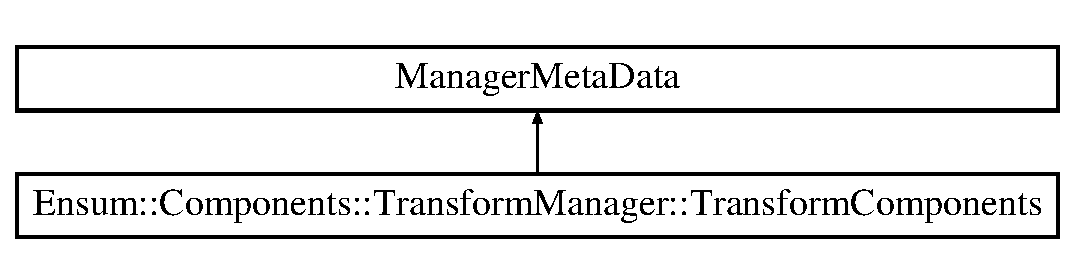
\includegraphics[height=2.000000cm]{struct_ensum_1_1_components_1_1_transform_manager_1_1_transform_components}
\end{center}
\end{figure}
\subsection*{Public Attributes}
\begin{DoxyCompactItemize}
\item 
uint32\+\_\+t $\ast$ {\bfseries Parent}\hypertarget{struct_ensum_1_1_components_1_1_transform_manager_1_1_transform_components_a5521d2c518d7041535f226b28874cdcb}{}\label{struct_ensum_1_1_components_1_1_transform_manager_1_1_transform_components_a5521d2c518d7041535f226b28874cdcb}

\item 
uint32\+\_\+t $\ast$ {\bfseries First\+Child}\hypertarget{struct_ensum_1_1_components_1_1_transform_manager_1_1_transform_components_aa9c06c787f56ea072473592ed7b6fd9f}{}\label{struct_ensum_1_1_components_1_1_transform_manager_1_1_transform_components_aa9c06c787f56ea072473592ed7b6fd9f}

\item 
uint32\+\_\+t $\ast$ {\bfseries Prev\+Sibling}\hypertarget{struct_ensum_1_1_components_1_1_transform_manager_1_1_transform_components_ae9de87772879d303fb2cf42113a0a558}{}\label{struct_ensum_1_1_components_1_1_transform_manager_1_1_transform_components_ae9de87772879d303fb2cf42113a0a558}

\item 
uint32\+\_\+t $\ast$ {\bfseries Next\+Sibling}\hypertarget{struct_ensum_1_1_components_1_1_transform_manager_1_1_transform_components_a42c6bd9613049f21132505a3f694f242}{}\label{struct_ensum_1_1_components_1_1_transform_manager_1_1_transform_components_a42c6bd9613049f21132505a3f694f242}

\item 
Direct\+X\+::\+X\+M\+F\+L\+O\+A\+T4\+X4 $\ast$ {\bfseries Local}\hypertarget{struct_ensum_1_1_components_1_1_transform_manager_1_1_transform_components_a848defbc0540144a0177485d1387e1a9}{}\label{struct_ensum_1_1_components_1_1_transform_manager_1_1_transform_components_a848defbc0540144a0177485d1387e1a9}

\item 
Direct\+X\+::\+X\+M\+F\+L\+O\+A\+T4\+X4 $\ast$ {\bfseries World}\hypertarget{struct_ensum_1_1_components_1_1_transform_manager_1_1_transform_components_a29b6e674a5ac14c8da5646852e5f56a1}{}\label{struct_ensum_1_1_components_1_1_transform_manager_1_1_transform_components_a29b6e674a5ac14c8da5646852e5f56a1}

\item 
Direct\+X\+::\+X\+M\+F\+L\+O\+A\+T3 $\ast$ {\bfseries PositionL}\hypertarget{struct_ensum_1_1_components_1_1_transform_manager_1_1_transform_components_a56500c57a61de78e350b092e9cc9419f}{}\label{struct_ensum_1_1_components_1_1_transform_manager_1_1_transform_components_a56500c57a61de78e350b092e9cc9419f}

\item 
Direct\+X\+::\+X\+M\+F\+L\+O\+A\+T3 $\ast$ {\bfseries Rotation}\hypertarget{struct_ensum_1_1_components_1_1_transform_manager_1_1_transform_components_ab977b81bd5c4233f30e883c1ee339a03}{}\label{struct_ensum_1_1_components_1_1_transform_manager_1_1_transform_components_ab977b81bd5c4233f30e883c1ee339a03}

\item 
Direct\+X\+::\+X\+M\+F\+L\+O\+A\+T3 $\ast$ {\bfseries Scale}\hypertarget{struct_ensum_1_1_components_1_1_transform_manager_1_1_transform_components_a733a0915ffb74c4bf78e68815c297143}{}\label{struct_ensum_1_1_components_1_1_transform_manager_1_1_transform_components_a733a0915ffb74c4bf78e68815c297143}

\item 
Direct\+X\+::\+X\+M\+F\+L\+O\+A\+T3 $\ast$ {\bfseries Forward}\hypertarget{struct_ensum_1_1_components_1_1_transform_manager_1_1_transform_components_a579f47d23db64d88b47e9faf6735c92b}{}\label{struct_ensum_1_1_components_1_1_transform_manager_1_1_transform_components_a579f47d23db64d88b47e9faf6735c92b}

\item 
Direct\+X\+::\+X\+M\+F\+L\+O\+A\+T3 $\ast$ {\bfseries Up}\hypertarget{struct_ensum_1_1_components_1_1_transform_manager_1_1_transform_components_a622847ecf1ee6bacf788f24d041d0b57}{}\label{struct_ensum_1_1_components_1_1_transform_manager_1_1_transform_components_a622847ecf1ee6bacf788f24d041d0b57}

\item 
Direct\+X\+::\+X\+M\+F\+L\+O\+A\+T3 $\ast$ {\bfseries Right}\hypertarget{struct_ensum_1_1_components_1_1_transform_manager_1_1_transform_components_a221c35ddae06ba1f19c54bea7fe62168}{}\label{struct_ensum_1_1_components_1_1_transform_manager_1_1_transform_components_a221c35ddae06ba1f19c54bea7fe62168}

\end{DoxyCompactItemize}


\subsection{Detailed Description}
The managers data struct. 

The documentation for this struct was generated from the following file\+:\begin{DoxyCompactItemize}
\item 
C\+:/\+Users/peter/\+Source/\+Repos/\+E\+N\+S\+U\+M/\+Ensum/\+Includes/\+Ensum\+\_\+components/Transform\+Manager.\+h\end{DoxyCompactItemize}

\hypertarget{class_ensum_1_1_components_1_1_transform_manager}{}\section{Ensum\+:\+:Components\+:\+:Transform\+Manager Class Reference}
\label{class_ensum_1_1_components_1_1_transform_manager}\index{Ensum\+::\+Components\+::\+Transform\+Manager@{Ensum\+::\+Components\+::\+Transform\+Manager}}


Handles the transform of the entities.  




{\ttfamily \#include $<$Transform\+Manager.\+h$>$}

Inheritance diagram for Ensum\+:\+:Components\+:\+:Transform\+Manager\+:\begin{figure}[H]
\begin{center}
\leavevmode
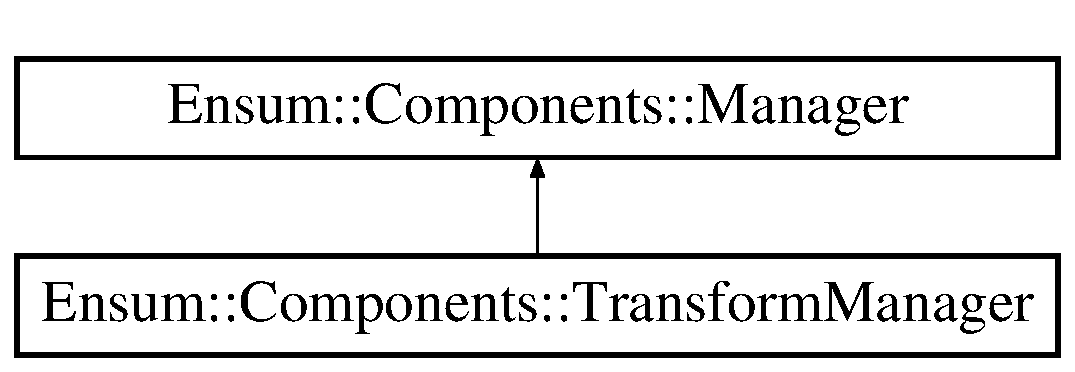
\includegraphics[height=2.000000cm]{class_ensum_1_1_components_1_1_transform_manager}
\end{center}
\end{figure}
\subsection*{Classes}
\begin{DoxyCompactItemize}
\item 
struct \hyperlink{struct_ensum_1_1_components_1_1_transform_manager_1_1_transform_components}{Transform\+Components}
\begin{DoxyCompactList}\small\item\em The managers data struct. \end{DoxyCompactList}\end{DoxyCompactItemize}
\subsection*{Public Member Functions}
\begin{DoxyCompactItemize}
\item 
{\bfseries Transform\+Manager} (\hyperlink{class_ensum_1_1_components_1_1_entity_manager}{Entity\+Manager} \&ent\+Manager)\hypertarget{class_ensum_1_1_components_1_1_transform_manager_a6d9111abc5ab4fba9e31cf7b8096233b}{}\label{class_ensum_1_1_components_1_1_transform_manager_a6d9111abc5ab4fba9e31cf7b8096233b}

\item 
const void \hyperlink{class_ensum_1_1_components_1_1_transform_manager_a484089df7e71d762e6df10d70df01b97}{Create\+Transform} (const \hyperlink{struct_ensum_1_1_components_1_1_entity}{Entity} \&entity)\hypertarget{class_ensum_1_1_components_1_1_transform_manager_a484089df7e71d762e6df10d70df01b97}{}\label{class_ensum_1_1_components_1_1_transform_manager_a484089df7e71d762e6df10d70df01b97}

\begin{DoxyCompactList}\small\item\em Create a transform component for the entity. \end{DoxyCompactList}\item 
const void \hyperlink{class_ensum_1_1_components_1_1_transform_manager_a2d240e72b697be19aecae1527599480e}{Bind\+Child} (const \hyperlink{struct_ensum_1_1_components_1_1_entity}{Entity} \&parent, const \hyperlink{struct_ensum_1_1_components_1_1_entity}{Entity} \&child, bool relative\+To\+Parent=false)
\begin{DoxyCompactList}\small\item\em Bind a entity as child to another. \end{DoxyCompactList}\item 
const void \hyperlink{class_ensum_1_1_components_1_1_transform_manager_ab7dc49fe8a330efbe10c8b55f0bc0398}{Unbind\+Child} (const \hyperlink{struct_ensum_1_1_components_1_1_entity}{Entity} \&child)
\begin{DoxyCompactList}\small\item\em Unbind an entity as child. \end{DoxyCompactList}\item 
const void \hyperlink{class_ensum_1_1_components_1_1_transform_manager_a62314eeafd1d1368b82b1ea3002d3a71}{Move} (const \hyperlink{struct_ensum_1_1_components_1_1_entity}{Entity} \&entity, const Direct\+X\+::\+X\+M\+F\+L\+O\+A\+T3 \&direction)
\begin{DoxyCompactList}\small\item\em Move forward-\/x, right-\/y, up-\/z. \end{DoxyCompactList}\item 
const void {\bfseries Move\+Forward} (const \hyperlink{struct_ensum_1_1_components_1_1_entity}{Entity} \&entity, const float amount)\hypertarget{class_ensum_1_1_components_1_1_transform_manager_ae1748b0c5be7ff6c45ded730504f1b2e}{}\label{class_ensum_1_1_components_1_1_transform_manager_ae1748b0c5be7ff6c45ded730504f1b2e}

\item 
const void {\bfseries Move\+Backward} (const \hyperlink{struct_ensum_1_1_components_1_1_entity}{Entity} \&entity, const float amount)\hypertarget{class_ensum_1_1_components_1_1_transform_manager_a7a9d054f27c3b05bd8622e88f476142c}{}\label{class_ensum_1_1_components_1_1_transform_manager_a7a9d054f27c3b05bd8622e88f476142c}

\item 
const void {\bfseries Move\+Right} (const \hyperlink{struct_ensum_1_1_components_1_1_entity}{Entity} \&entity, const float amount)\hypertarget{class_ensum_1_1_components_1_1_transform_manager_a9155f3880b1ac2ef76fbf2e77d56537c}{}\label{class_ensum_1_1_components_1_1_transform_manager_a9155f3880b1ac2ef76fbf2e77d56537c}

\item 
const void {\bfseries Move\+Left} (const \hyperlink{struct_ensum_1_1_components_1_1_entity}{Entity} \&entity, const float amount)\hypertarget{class_ensum_1_1_components_1_1_transform_manager_a9e65ded7e7f3eb7415534c8e25f75502}{}\label{class_ensum_1_1_components_1_1_transform_manager_a9e65ded7e7f3eb7415534c8e25f75502}

\item 
const void {\bfseries Move\+Up} (const \hyperlink{struct_ensum_1_1_components_1_1_entity}{Entity} \&entity, const float amount)\hypertarget{class_ensum_1_1_components_1_1_transform_manager_a41e6739af3127f254d0ba4b3d6d5467b}{}\label{class_ensum_1_1_components_1_1_transform_manager_a41e6739af3127f254d0ba4b3d6d5467b}

\item 
const void {\bfseries Move\+Down} (const \hyperlink{struct_ensum_1_1_components_1_1_entity}{Entity} \&entity, const float amount)\hypertarget{class_ensum_1_1_components_1_1_transform_manager_a675ee13a589930176c0b5bf4c3fa0a04}{}\label{class_ensum_1_1_components_1_1_transform_manager_a675ee13a589930176c0b5bf4c3fa0a04}

\item 
const void {\bfseries Move\+Along\+Vector} (const \hyperlink{struct_ensum_1_1_components_1_1_entity}{Entity} \&entity, const Direct\+X\+::\+X\+M\+V\+E\+C\+T\+OR amount)\hypertarget{class_ensum_1_1_components_1_1_transform_manager_a243adff170f09f90e170cdce154c1434}{}\label{class_ensum_1_1_components_1_1_transform_manager_a243adff170f09f90e170cdce154c1434}

\item 
const void {\bfseries Move\+Along\+Vector} (const \hyperlink{struct_ensum_1_1_components_1_1_entity}{Entity} \&entity, Direct\+X\+::\+X\+M\+V\+E\+C\+T\+OR dir, float amount)\hypertarget{class_ensum_1_1_components_1_1_transform_manager_a53f28a815293ffa0c2f07d03a594c54e}{}\label{class_ensum_1_1_components_1_1_transform_manager_a53f28a815293ffa0c2f07d03a594c54e}

\item 
const void {\bfseries Rotate} (const \hyperlink{struct_ensum_1_1_components_1_1_entity}{Entity} \&entity, const Direct\+X\+::\+X\+M\+F\+L\+O\+A\+T3 \&radians)\hypertarget{class_ensum_1_1_components_1_1_transform_manager_af12d20ba876189b13c67b8ab056993b5}{}\label{class_ensum_1_1_components_1_1_transform_manager_af12d20ba876189b13c67b8ab056993b5}

\item 
const void {\bfseries Rotate\+Yaw} (const \hyperlink{struct_ensum_1_1_components_1_1_entity}{Entity} \&entity, const float radians)\hypertarget{class_ensum_1_1_components_1_1_transform_manager_a1fca568d1223c92a34e41b0d2b02f46a}{}\label{class_ensum_1_1_components_1_1_transform_manager_a1fca568d1223c92a34e41b0d2b02f46a}

\item 
const void {\bfseries Rotate\+Pitch} (const \hyperlink{struct_ensum_1_1_components_1_1_entity}{Entity} \&entity, const float radians)\hypertarget{class_ensum_1_1_components_1_1_transform_manager_a4fe43a20b760088ab0a8eddf64d70e21}{}\label{class_ensum_1_1_components_1_1_transform_manager_a4fe43a20b760088ab0a8eddf64d70e21}

\item 
const void {\bfseries Rotate\+Roll} (const \hyperlink{struct_ensum_1_1_components_1_1_entity}{Entity} \&entity, const float radians)\hypertarget{class_ensum_1_1_components_1_1_transform_manager_ad7a14a0b253c62017263d6a92e911e10}{}\label{class_ensum_1_1_components_1_1_transform_manager_ad7a14a0b253c62017263d6a92e911e10}

\item 
const void {\bfseries Set\+Position} (const \hyperlink{struct_ensum_1_1_components_1_1_entity}{Entity} \&entity, const Direct\+X\+::\+X\+M\+F\+L\+O\+A\+T3 \&position, bool relative\+To\+Parent=false)\hypertarget{class_ensum_1_1_components_1_1_transform_manager_a401b2f17c82370f173c034d78b7fd700}{}\label{class_ensum_1_1_components_1_1_transform_manager_a401b2f17c82370f173c034d78b7fd700}

\item 
const void {\bfseries Set\+Position} (const \hyperlink{struct_ensum_1_1_components_1_1_entity}{Entity} \&entity, const Direct\+X\+::\+X\+M\+V\+E\+C\+T\+OR \&position, bool relative\+To\+Parent=false)\hypertarget{class_ensum_1_1_components_1_1_transform_manager_a1b930b81981049c5394f188baab3c1bd}{}\label{class_ensum_1_1_components_1_1_transform_manager_a1b930b81981049c5394f188baab3c1bd}

\item 
const void {\bfseries Set\+Rotation} (const \hyperlink{struct_ensum_1_1_components_1_1_entity}{Entity} \&entity, const Direct\+X\+::\+X\+M\+F\+L\+O\+A\+T3 \&rotation)\hypertarget{class_ensum_1_1_components_1_1_transform_manager_ac770f58d61a7369814e607b43072824f}{}\label{class_ensum_1_1_components_1_1_transform_manager_ac770f58d61a7369814e607b43072824f}

\item 
const void {\bfseries Set\+Rotation} (const \hyperlink{struct_ensum_1_1_components_1_1_entity}{Entity} \&entity, const Direct\+X\+::\+X\+M\+V\+E\+C\+T\+OR \&rotation)\hypertarget{class_ensum_1_1_components_1_1_transform_manager_a2a4e2c7374de1f26f6ac7fca0b22c9de}{}\label{class_ensum_1_1_components_1_1_transform_manager_a2a4e2c7374de1f26f6ac7fca0b22c9de}

\item 
const void {\bfseries Set\+Scale} (const \hyperlink{struct_ensum_1_1_components_1_1_entity}{Entity} \&entity, const Direct\+X\+::\+X\+M\+F\+L\+O\+A\+T3 \&scale, bool relative\+To\+Parent=false)\hypertarget{class_ensum_1_1_components_1_1_transform_manager_a0b4cf5a20533bf1efb65fbc0e9c9d3bf}{}\label{class_ensum_1_1_components_1_1_transform_manager_a0b4cf5a20533bf1efb65fbc0e9c9d3bf}

\item 
const void {\bfseries Set\+Scale} (const \hyperlink{struct_ensum_1_1_components_1_1_entity}{Entity} \&entity, const Direct\+X\+::\+X\+M\+V\+E\+C\+T\+OR \&scale, bool relative\+To\+Parent=false)\hypertarget{class_ensum_1_1_components_1_1_transform_manager_afc32dc7d90e2a180f2d8cf0d5838fbc0}{}\label{class_ensum_1_1_components_1_1_transform_manager_afc32dc7d90e2a180f2d8cf0d5838fbc0}

\item 
const void {\bfseries Set\+Forward} (const \hyperlink{struct_ensum_1_1_components_1_1_entity}{Entity} \&entity, const Direct\+X\+::\+X\+M\+F\+L\+O\+A\+T3 \&forward, bool relative\+To\+Parent=false)\hypertarget{class_ensum_1_1_components_1_1_transform_manager_ac6f1ab9da36867b8ceadf235e1029893}{}\label{class_ensum_1_1_components_1_1_transform_manager_ac6f1ab9da36867b8ceadf235e1029893}

\item 
const void {\bfseries Set\+Forward} (const \hyperlink{struct_ensum_1_1_components_1_1_entity}{Entity} \&entity, const Direct\+X\+::\+X\+M\+V\+E\+C\+T\+OR \&forward, bool relative\+To\+Parent=false)\hypertarget{class_ensum_1_1_components_1_1_transform_manager_ab28a6fe03a0e3da6098006e52655a924}{}\label{class_ensum_1_1_components_1_1_transform_manager_ab28a6fe03a0e3da6098006e52655a924}

\item 
const Direct\+X\+::\+X\+M\+V\+E\+C\+T\+OR {\bfseries Get\+Position} (const \hyperlink{struct_ensum_1_1_components_1_1_entity}{Entity} \&entity)\hypertarget{class_ensum_1_1_components_1_1_transform_manager_a1f88872efff1d4f46e96b9eb1f1ad42a}{}\label{class_ensum_1_1_components_1_1_transform_manager_a1f88872efff1d4f46e96b9eb1f1ad42a}

\item 
const Direct\+X\+::\+X\+M\+V\+E\+C\+T\+OR {\bfseries Get\+Rotation} (const \hyperlink{struct_ensum_1_1_components_1_1_entity}{Entity} \&entity)\hypertarget{class_ensum_1_1_components_1_1_transform_manager_a63544a06e7e1092d99c2f41bb19f8016}{}\label{class_ensum_1_1_components_1_1_transform_manager_a63544a06e7e1092d99c2f41bb19f8016}

\item 
const Direct\+X\+::\+X\+M\+V\+E\+C\+T\+OR {\bfseries Get\+Scale} (const \hyperlink{struct_ensum_1_1_components_1_1_entity}{Entity} \&entity)\hypertarget{class_ensum_1_1_components_1_1_transform_manager_a5d84f5fdf153d6097537fc04090d0004}{}\label{class_ensum_1_1_components_1_1_transform_manager_a5d84f5fdf153d6097537fc04090d0004}

\item 
const Direct\+X\+::\+X\+M\+V\+E\+C\+T\+OR {\bfseries Get\+Forward} (const \hyperlink{struct_ensum_1_1_components_1_1_entity}{Entity} \&entity)\hypertarget{class_ensum_1_1_components_1_1_transform_manager_ae952c3520ee76be6f170f7ca087fa14f}{}\label{class_ensum_1_1_components_1_1_transform_manager_ae952c3520ee76be6f170f7ca087fa14f}

\item 
const Direct\+X\+::\+X\+M\+V\+E\+C\+T\+OR {\bfseries Get\+Right} (const \hyperlink{struct_ensum_1_1_components_1_1_entity}{Entity} \&entity)\hypertarget{class_ensum_1_1_components_1_1_transform_manager_a80bc26bf87027ec5c7cb3a9b8f4d2b45}{}\label{class_ensum_1_1_components_1_1_transform_manager_a80bc26bf87027ec5c7cb3a9b8f4d2b45}

\item 
const Direct\+X\+::\+X\+M\+V\+E\+C\+T\+OR {\bfseries Get\+Up} (const \hyperlink{struct_ensum_1_1_components_1_1_entity}{Entity} \&entity)\hypertarget{class_ensum_1_1_components_1_1_transform_manager_a0915707915f8e5443a1e37b2f1121aae}{}\label{class_ensum_1_1_components_1_1_transform_manager_a0915707915f8e5443a1e37b2f1121aae}

\end{DoxyCompactItemize}
\subsection*{Private Member Functions}
\begin{DoxyCompactItemize}
\item 
const void \hyperlink{class_ensum_1_1_components_1_1_transform_manager_a90703a5b97caaafee225459ca872c446}{\+\_\+\+Allocate} (uint32\+\_\+t size)
\begin{DoxyCompactList}\small\item\em Allocate more memory. \end{DoxyCompactList}\item 
const void \hyperlink{class_ensum_1_1_components_1_1_transform_manager_a47f354c8a26b83d12809611516be65c7}{\+\_\+\+Destroy} (uint32\+\_\+t index)
\begin{DoxyCompactList}\small\item\em Delete an entry in the memory block. \end{DoxyCompactList}\item 
const uint32\+\_\+t \hyperlink{class_ensum_1_1_components_1_1_transform_manager_a68fa8f539fb52e6945dd82902b61b3c5}{\+\_\+\+Create\+Transform} (const \hyperlink{struct_ensum_1_1_components_1_1_entity}{Entity} \&entity)
\begin{DoxyCompactList}\small\item\em Create a transform component for the entity. \end{DoxyCompactList}\item 
const void \hyperlink{class_ensum_1_1_components_1_1_transform_manager_a7222458e2c7ec382f73343a67aa0aee6}{\+\_\+\+Bind\+Child} (uint32\+\_\+t parent, uint32\+\_\+t child, bool relative\+To\+Parent)
\begin{DoxyCompactList}\small\item\em Bind a entity as child to another. \end{DoxyCompactList}\item 
const void \hyperlink{class_ensum_1_1_components_1_1_transform_manager_a08e37f57af9622645b28139b4f7e3792}{\+\_\+\+Unbind\+Child} (uint32\+\_\+t child)
\begin{DoxyCompactList}\small\item\em Unbind an entity as child. \end{DoxyCompactList}\item 
const void \hyperlink{class_ensum_1_1_components_1_1_transform_manager_a62fe544a73f4a09469d79872f8611024}{\+\_\+\+Move} (uint32\+\_\+t index, const Direct\+X\+::\+X\+M\+F\+L\+O\+A\+T3 \&direction)
\begin{DoxyCompactList}\small\item\em Move forward-\/x, right-\/y, up-\/z. \end{DoxyCompactList}\item 
const void {\bfseries \+\_\+\+Move\+Forward} (uint32\+\_\+t index, const float amount)\hypertarget{class_ensum_1_1_components_1_1_transform_manager_aa39d072fd2599b7a5ebd62bc272996ba}{}\label{class_ensum_1_1_components_1_1_transform_manager_aa39d072fd2599b7a5ebd62bc272996ba}

\item 
const void {\bfseries \+\_\+\+Move\+Backward} (uint32\+\_\+t index, const float amount)\hypertarget{class_ensum_1_1_components_1_1_transform_manager_a50656a39c711957ab5269e67f3f0c5e9}{}\label{class_ensum_1_1_components_1_1_transform_manager_a50656a39c711957ab5269e67f3f0c5e9}

\item 
const void {\bfseries \+\_\+\+Move\+Right} (uint32\+\_\+t index, const float amount)\hypertarget{class_ensum_1_1_components_1_1_transform_manager_a200e1df71fffc9bf21212a3c92d71cc6}{}\label{class_ensum_1_1_components_1_1_transform_manager_a200e1df71fffc9bf21212a3c92d71cc6}

\item 
const void {\bfseries \+\_\+\+Move\+Left} (uint32\+\_\+t index, const float amount)\hypertarget{class_ensum_1_1_components_1_1_transform_manager_aed03886aff53b5937ff458f4fe8bd135}{}\label{class_ensum_1_1_components_1_1_transform_manager_aed03886aff53b5937ff458f4fe8bd135}

\item 
const void {\bfseries \+\_\+\+Move\+Up} (uint32\+\_\+t index, const float amount)\hypertarget{class_ensum_1_1_components_1_1_transform_manager_aefdabf28a594cfbee912e7c33dc3904f}{}\label{class_ensum_1_1_components_1_1_transform_manager_aefdabf28a594cfbee912e7c33dc3904f}

\item 
const void {\bfseries \+\_\+\+Move\+Down} (uint32\+\_\+t index, const float amount)\hypertarget{class_ensum_1_1_components_1_1_transform_manager_a2eacf57922ea1a0fdba9817e783d11b6}{}\label{class_ensum_1_1_components_1_1_transform_manager_a2eacf57922ea1a0fdba9817e783d11b6}

\item 
const void {\bfseries \+\_\+\+Move\+Along\+Vector} (uint32\+\_\+t index, const Direct\+X\+::\+X\+M\+V\+E\+C\+T\+OR amount)\hypertarget{class_ensum_1_1_components_1_1_transform_manager_ad4ed93621abcdd070336fccffd160333}{}\label{class_ensum_1_1_components_1_1_transform_manager_ad4ed93621abcdd070336fccffd160333}

\item 
const void {\bfseries \+\_\+\+Move\+Along\+Vector} (uint32\+\_\+t index, Direct\+X\+::\+X\+M\+V\+E\+C\+T\+OR dir, float amount)\hypertarget{class_ensum_1_1_components_1_1_transform_manager_aef05093bb6428418b461151150b00c50}{}\label{class_ensum_1_1_components_1_1_transform_manager_aef05093bb6428418b461151150b00c50}

\item 
const void {\bfseries \+\_\+\+Rotate} (uint32\+\_\+t index, const Direct\+X\+::\+X\+M\+F\+L\+O\+A\+T3 \&radians)\hypertarget{class_ensum_1_1_components_1_1_transform_manager_a94e359a45bfaa598f8c08b9e31cc8025}{}\label{class_ensum_1_1_components_1_1_transform_manager_a94e359a45bfaa598f8c08b9e31cc8025}

\item 
const void {\bfseries \+\_\+\+Rotate\+Yaw} (uint32\+\_\+t index, const float radians)\hypertarget{class_ensum_1_1_components_1_1_transform_manager_a54777efdcd5b6d082cc20147c21e5348}{}\label{class_ensum_1_1_components_1_1_transform_manager_a54777efdcd5b6d082cc20147c21e5348}

\item 
const void {\bfseries \+\_\+\+Rotate\+Pitch} (uint32\+\_\+t index, const float radians)\hypertarget{class_ensum_1_1_components_1_1_transform_manager_ae46a70a55aa5f080b15f2290633f243d}{}\label{class_ensum_1_1_components_1_1_transform_manager_ae46a70a55aa5f080b15f2290633f243d}

\item 
const void {\bfseries \+\_\+\+Rotate\+Roll} (uint32\+\_\+t index, const float radians)\hypertarget{class_ensum_1_1_components_1_1_transform_manager_a64bbc7d142674869532b422c57b31a11}{}\label{class_ensum_1_1_components_1_1_transform_manager_a64bbc7d142674869532b422c57b31a11}

\item 
const void {\bfseries \+\_\+\+Set\+Position} (uint32\+\_\+t index, const Direct\+X\+::\+X\+M\+F\+L\+O\+A\+T3 \&position, bool relative\+To\+Parent=false)\hypertarget{class_ensum_1_1_components_1_1_transform_manager_a830889e8aa1ab8dd5c84c1da08a65eca}{}\label{class_ensum_1_1_components_1_1_transform_manager_a830889e8aa1ab8dd5c84c1da08a65eca}

\item 
const void {\bfseries \+\_\+\+Set\+Position} (uint32\+\_\+t index, const Direct\+X\+::\+X\+M\+V\+E\+C\+T\+OR \&position, bool relative\+To\+Parent=false)\hypertarget{class_ensum_1_1_components_1_1_transform_manager_a77609ace7a0622232b84a60d236fb75c}{}\label{class_ensum_1_1_components_1_1_transform_manager_a77609ace7a0622232b84a60d236fb75c}

\item 
const void {\bfseries \+\_\+\+Set\+Rotation} (uint32\+\_\+t index, const Direct\+X\+::\+X\+M\+F\+L\+O\+A\+T3 \&rotation)\hypertarget{class_ensum_1_1_components_1_1_transform_manager_a802d57c893c0c261b3f12702ab52943f}{}\label{class_ensum_1_1_components_1_1_transform_manager_a802d57c893c0c261b3f12702ab52943f}

\item 
const void {\bfseries \+\_\+\+Set\+Rotation} (uint32\+\_\+t index, const Direct\+X\+::\+X\+M\+V\+E\+C\+T\+OR \&rotation)\hypertarget{class_ensum_1_1_components_1_1_transform_manager_a4bc5b1864100fc3cf85fe50d8719f07e}{}\label{class_ensum_1_1_components_1_1_transform_manager_a4bc5b1864100fc3cf85fe50d8719f07e}

\item 
const void {\bfseries \+\_\+\+Set\+Scale} (uint32\+\_\+t index, const Direct\+X\+::\+X\+M\+F\+L\+O\+A\+T3 \&scale, bool relative\+To\+Parent=false)\hypertarget{class_ensum_1_1_components_1_1_transform_manager_a0c99c23b7e4329a4717021394fa9e4b9}{}\label{class_ensum_1_1_components_1_1_transform_manager_a0c99c23b7e4329a4717021394fa9e4b9}

\item 
const void {\bfseries \+\_\+\+Set\+Scale} (uint32\+\_\+t index, const Direct\+X\+::\+X\+M\+V\+E\+C\+T\+OR \&scale, bool relative\+To\+Parent=false)\hypertarget{class_ensum_1_1_components_1_1_transform_manager_a77af7e15d39f11c5a5ea9608d36aab3a}{}\label{class_ensum_1_1_components_1_1_transform_manager_a77af7e15d39f11c5a5ea9608d36aab3a}

\item 
const void {\bfseries \+\_\+\+Set\+Forward} (uint32\+\_\+t index, const Direct\+X\+::\+X\+M\+F\+L\+O\+A\+T3 \&forward, bool relative\+To\+Parent=false)\hypertarget{class_ensum_1_1_components_1_1_transform_manager_a4d23fb876a394beb48d2c11531215897}{}\label{class_ensum_1_1_components_1_1_transform_manager_a4d23fb876a394beb48d2c11531215897}

\item 
const void {\bfseries \+\_\+\+Set\+Forward} (uint32\+\_\+t index, const Direct\+X\+::\+X\+M\+V\+E\+C\+T\+OR \&forward, bool relative\+To\+Parent=false)\hypertarget{class_ensum_1_1_components_1_1_transform_manager_af6e6e9cd9eb807841adb9828c5e0fa8e}{}\label{class_ensum_1_1_components_1_1_transform_manager_af6e6e9cd9eb807841adb9828c5e0fa8e}

\item 
const Direct\+X\+::\+X\+M\+V\+E\+C\+T\+OR {\bfseries \+\_\+\+Get\+Position} (uint32\+\_\+t index)\hypertarget{class_ensum_1_1_components_1_1_transform_manager_a96b1da90d26422c620abaab2f3d496fc}{}\label{class_ensum_1_1_components_1_1_transform_manager_a96b1da90d26422c620abaab2f3d496fc}

\item 
const Direct\+X\+::\+X\+M\+V\+E\+C\+T\+OR {\bfseries \+\_\+\+Get\+Rotation} (uint32\+\_\+t index)\hypertarget{class_ensum_1_1_components_1_1_transform_manager_af09798cd8daa7a687e384004ebf697f5}{}\label{class_ensum_1_1_components_1_1_transform_manager_af09798cd8daa7a687e384004ebf697f5}

\item 
const Direct\+X\+::\+X\+M\+V\+E\+C\+T\+OR {\bfseries \+\_\+\+Get\+Scale} (uint32\+\_\+t index)\hypertarget{class_ensum_1_1_components_1_1_transform_manager_a05cdff28571a120d279fd0428f08b5fd}{}\label{class_ensum_1_1_components_1_1_transform_manager_a05cdff28571a120d279fd0428f08b5fd}

\item 
const Direct\+X\+::\+X\+M\+V\+E\+C\+T\+OR {\bfseries \+\_\+\+Get\+Forward} (uint32\+\_\+t index)\hypertarget{class_ensum_1_1_components_1_1_transform_manager_aa137f5b348c0c8844abce56c47b5f564}{}\label{class_ensum_1_1_components_1_1_transform_manager_aa137f5b348c0c8844abce56c47b5f564}

\item 
const Direct\+X\+::\+X\+M\+V\+E\+C\+T\+OR {\bfseries \+\_\+\+Get\+Right} (uint32\+\_\+t index)\hypertarget{class_ensum_1_1_components_1_1_transform_manager_aba2e3fb3988acbcd49d07d2299e0a93d}{}\label{class_ensum_1_1_components_1_1_transform_manager_aba2e3fb3988acbcd49d07d2299e0a93d}

\item 
const Direct\+X\+::\+X\+M\+V\+E\+C\+T\+OR {\bfseries \+\_\+\+Get\+Up} (uint32\+\_\+t index)\hypertarget{class_ensum_1_1_components_1_1_transform_manager_a52a759a25c0129168670fc572693656f}{}\label{class_ensum_1_1_components_1_1_transform_manager_a52a759a25c0129168670fc572693656f}

\item 
const void \hyperlink{class_ensum_1_1_components_1_1_transform_manager_a50bed80577a1a6b97b9dbbf1fea2bc93}{\+\_\+\+Transform\+To\+Parent\+Local} (uint32\+\_\+t parent, uint32\+\_\+t child)
\begin{DoxyCompactList}\small\item\em Transform to parents local. \end{DoxyCompactList}\item 
const void \hyperlink{class_ensum_1_1_components_1_1_transform_manager_a860ac4eb9d36ae8c4077225f8323102f}{\+\_\+\+Transform\+From\+Parent\+Local} (uint32\+\_\+t parent, uint32\+\_\+t child)
\begin{DoxyCompactList}\small\item\em Transform from parents local. \end{DoxyCompactList}\item 
const void \hyperlink{class_ensum_1_1_components_1_1_transform_manager_abba8eea1db8554cb1aba12bc7eb57d1d}{\+\_\+\+Transform} (uint32\+\_\+t index)
\begin{DoxyCompactList}\small\item\em Transform has changed, so update everything. \end{DoxyCompactList}\end{DoxyCompactItemize}
\subsection*{Private Attributes}
\begin{DoxyCompactItemize}
\item 
\hyperlink{struct_ensum_1_1_components_1_1_transform_manager_1_1_transform_components}{Transform\+Components} $\ast$ \hyperlink{class_ensum_1_1_components_1_1_transform_manager_aacb8cd9eb6f473b5b83f48c69a5e893d}{\+\_\+datap}
\end{DoxyCompactItemize}
\subsection*{Friends}
\begin{DoxyCompactItemize}
\item 
class {\bfseries Camera\+Manager}\hypertarget{class_ensum_1_1_components_1_1_transform_manager_afae5bf9a900e8c5bc70c9332785e8465}{}\label{class_ensum_1_1_components_1_1_transform_manager_afae5bf9a900e8c5bc70c9332785e8465}

\end{DoxyCompactItemize}
\subsection*{Additional Inherited Members}


\subsection{Detailed Description}
Handles the transform of the entities. 

\subsection{Member Function Documentation}
\index{Ensum\+::\+Components\+::\+Transform\+Manager@{Ensum\+::\+Components\+::\+Transform\+Manager}!\+\_\+\+Allocate@{\+\_\+\+Allocate}}
\index{\+\_\+\+Allocate@{\+\_\+\+Allocate}!Ensum\+::\+Components\+::\+Transform\+Manager@{Ensum\+::\+Components\+::\+Transform\+Manager}}
\subsubsection[{\texorpdfstring{\+\_\+\+Allocate(uint32\+\_\+t size)}{_Allocate(uint32_t size)}}]{\setlength{\rightskip}{0pt plus 5cm}const void Ensum\+::\+Components\+::\+Transform\+Manager\+::\+\_\+\+Allocate (
\begin{DoxyParamCaption}
\item[{uint32\+\_\+t}]{size}
\end{DoxyParamCaption}
)\hspace{0.3cm}{\ttfamily [private]}, {\ttfamily [virtual]}}\hypertarget{class_ensum_1_1_components_1_1_transform_manager_a90703a5b97caaafee225459ca872c446}{}\label{class_ensum_1_1_components_1_1_transform_manager_a90703a5b97caaafee225459ca872c446}


Allocate more memory. 



Implements \hyperlink{class_ensum_1_1_components_1_1_manager_a1b593059210d09632c910a6abaae49c0}{Ensum\+::\+Components\+::\+Manager}.

\index{Ensum\+::\+Components\+::\+Transform\+Manager@{Ensum\+::\+Components\+::\+Transform\+Manager}!\+\_\+\+Bind\+Child@{\+\_\+\+Bind\+Child}}
\index{\+\_\+\+Bind\+Child@{\+\_\+\+Bind\+Child}!Ensum\+::\+Components\+::\+Transform\+Manager@{Ensum\+::\+Components\+::\+Transform\+Manager}}
\subsubsection[{\texorpdfstring{\+\_\+\+Bind\+Child(uint32\+\_\+t parent, uint32\+\_\+t child, bool relative\+To\+Parent)}{_BindChild(uint32_t parent, uint32_t child, bool relativeToParent)}}]{\setlength{\rightskip}{0pt plus 5cm}const void Ensum\+::\+Components\+::\+Transform\+Manager\+::\+\_\+\+Bind\+Child (
\begin{DoxyParamCaption}
\item[{uint32\+\_\+t}]{parent, }
\item[{uint32\+\_\+t}]{child, }
\item[{bool}]{relative\+To\+Parent}
\end{DoxyParamCaption}
)\hspace{0.3cm}{\ttfamily [private]}}\hypertarget{class_ensum_1_1_components_1_1_transform_manager_a7222458e2c7ec382f73343a67aa0aee6}{}\label{class_ensum_1_1_components_1_1_transform_manager_a7222458e2c7ec382f73343a67aa0aee6}


Bind a entity as child to another. 

(The private version.) If relative\+To\+Parent is true, the current local pos of the child will be the same. If relative\+To\+Parent is false, the local pos of the child will be translated to the parents space. It is assumed that the indices exist. Think of it as welding the entity to the parent. \index{Ensum\+::\+Components\+::\+Transform\+Manager@{Ensum\+::\+Components\+::\+Transform\+Manager}!\+\_\+\+Create\+Transform@{\+\_\+\+Create\+Transform}}
\index{\+\_\+\+Create\+Transform@{\+\_\+\+Create\+Transform}!Ensum\+::\+Components\+::\+Transform\+Manager@{Ensum\+::\+Components\+::\+Transform\+Manager}}
\subsubsection[{\texorpdfstring{\+\_\+\+Create\+Transform(const Entity \&entity)}{_CreateTransform(const Entity &entity)}}]{\setlength{\rightskip}{0pt plus 5cm}const uint32\+\_\+t Ensum\+::\+Components\+::\+Transform\+Manager\+::\+\_\+\+Create\+Transform (
\begin{DoxyParamCaption}
\item[{const {\bf Entity} \&}]{entity}
\end{DoxyParamCaption}
)\hspace{0.3cm}{\ttfamily [private]}}\hypertarget{class_ensum_1_1_components_1_1_transform_manager_a68fa8f539fb52e6945dd82902b61b3c5}{}\label{class_ensum_1_1_components_1_1_transform_manager_a68fa8f539fb52e6945dd82902b61b3c5}


Create a transform component for the entity. 

(The private version.) \index{Ensum\+::\+Components\+::\+Transform\+Manager@{Ensum\+::\+Components\+::\+Transform\+Manager}!\+\_\+\+Destroy@{\+\_\+\+Destroy}}
\index{\+\_\+\+Destroy@{\+\_\+\+Destroy}!Ensum\+::\+Components\+::\+Transform\+Manager@{Ensum\+::\+Components\+::\+Transform\+Manager}}
\subsubsection[{\texorpdfstring{\+\_\+\+Destroy(uint32\+\_\+t index)}{_Destroy(uint32_t index)}}]{\setlength{\rightskip}{0pt plus 5cm}const void Ensum\+::\+Components\+::\+Transform\+Manager\+::\+\_\+\+Destroy (
\begin{DoxyParamCaption}
\item[{uint32\+\_\+t}]{index}
\end{DoxyParamCaption}
)\hspace{0.3cm}{\ttfamily [private]}, {\ttfamily [virtual]}}\hypertarget{class_ensum_1_1_components_1_1_transform_manager_a47f354c8a26b83d12809611516be65c7}{}\label{class_ensum_1_1_components_1_1_transform_manager_a47f354c8a26b83d12809611516be65c7}


Delete an entry in the memory block. 

The deleted entry is replaced by the last in the block. 

Implements \hyperlink{class_ensum_1_1_components_1_1_manager_a5ba85395802e942ed8904ca18951e6b0}{Ensum\+::\+Components\+::\+Manager}.

\index{Ensum\+::\+Components\+::\+Transform\+Manager@{Ensum\+::\+Components\+::\+Transform\+Manager}!\+\_\+\+Move@{\+\_\+\+Move}}
\index{\+\_\+\+Move@{\+\_\+\+Move}!Ensum\+::\+Components\+::\+Transform\+Manager@{Ensum\+::\+Components\+::\+Transform\+Manager}}
\subsubsection[{\texorpdfstring{\+\_\+\+Move(uint32\+\_\+t index, const Direct\+X\+::\+X\+M\+F\+L\+O\+A\+T3 \&direction)}{_Move(uint32_t index, const DirectX::XMFLOAT3 &direction)}}]{\setlength{\rightskip}{0pt plus 5cm}const void Ensum\+::\+Components\+::\+Transform\+Manager\+::\+\_\+\+Move (
\begin{DoxyParamCaption}
\item[{uint32\+\_\+t}]{index, }
\item[{const Direct\+X\+::\+X\+M\+F\+L\+O\+A\+T3 \&}]{direction}
\end{DoxyParamCaption}
)\hspace{0.3cm}{\ttfamily [private]}}\hypertarget{class_ensum_1_1_components_1_1_transform_manager_a62fe544a73f4a09469d79872f8611024}{}\label{class_ensum_1_1_components_1_1_transform_manager_a62fe544a73f4a09469d79872f8611024}


Move forward-\/x, right-\/y, up-\/z. 

\index{Ensum\+::\+Components\+::\+Transform\+Manager@{Ensum\+::\+Components\+::\+Transform\+Manager}!\+\_\+\+Transform@{\+\_\+\+Transform}}
\index{\+\_\+\+Transform@{\+\_\+\+Transform}!Ensum\+::\+Components\+::\+Transform\+Manager@{Ensum\+::\+Components\+::\+Transform\+Manager}}
\subsubsection[{\texorpdfstring{\+\_\+\+Transform(uint32\+\_\+t index)}{_Transform(uint32_t index)}}]{\setlength{\rightskip}{0pt plus 5cm}const void Ensum\+::\+Components\+::\+Transform\+Manager\+::\+\_\+\+Transform (
\begin{DoxyParamCaption}
\item[{uint32\+\_\+t}]{index}
\end{DoxyParamCaption}
)\hspace{0.3cm}{\ttfamily [private]}}\hypertarget{class_ensum_1_1_components_1_1_transform_manager_abba8eea1db8554cb1aba12bc7eb57d1d}{}\label{class_ensum_1_1_components_1_1_transform_manager_abba8eea1db8554cb1aba12bc7eb57d1d}


Transform has changed, so update everything. 

It is assumed that the indices exist. \index{Ensum\+::\+Components\+::\+Transform\+Manager@{Ensum\+::\+Components\+::\+Transform\+Manager}!\+\_\+\+Transform\+From\+Parent\+Local@{\+\_\+\+Transform\+From\+Parent\+Local}}
\index{\+\_\+\+Transform\+From\+Parent\+Local@{\+\_\+\+Transform\+From\+Parent\+Local}!Ensum\+::\+Components\+::\+Transform\+Manager@{Ensum\+::\+Components\+::\+Transform\+Manager}}
\subsubsection[{\texorpdfstring{\+\_\+\+Transform\+From\+Parent\+Local(uint32\+\_\+t parent, uint32\+\_\+t child)}{_TransformFromParentLocal(uint32_t parent, uint32_t child)}}]{\setlength{\rightskip}{0pt plus 5cm}const void Ensum\+::\+Components\+::\+Transform\+Manager\+::\+\_\+\+Transform\+From\+Parent\+Local (
\begin{DoxyParamCaption}
\item[{uint32\+\_\+t}]{parent, }
\item[{uint32\+\_\+t}]{child}
\end{DoxyParamCaption}
)\hspace{0.3cm}{\ttfamily [private]}}\hypertarget{class_ensum_1_1_components_1_1_transform_manager_a860ac4eb9d36ae8c4077225f8323102f}{}\label{class_ensum_1_1_components_1_1_transform_manager_a860ac4eb9d36ae8c4077225f8323102f}


Transform from parents local. 

(The reverse of the above.) It is assumed that the indices exist. \index{Ensum\+::\+Components\+::\+Transform\+Manager@{Ensum\+::\+Components\+::\+Transform\+Manager}!\+\_\+\+Transform\+To\+Parent\+Local@{\+\_\+\+Transform\+To\+Parent\+Local}}
\index{\+\_\+\+Transform\+To\+Parent\+Local@{\+\_\+\+Transform\+To\+Parent\+Local}!Ensum\+::\+Components\+::\+Transform\+Manager@{Ensum\+::\+Components\+::\+Transform\+Manager}}
\subsubsection[{\texorpdfstring{\+\_\+\+Transform\+To\+Parent\+Local(uint32\+\_\+t parent, uint32\+\_\+t child)}{_TransformToParentLocal(uint32_t parent, uint32_t child)}}]{\setlength{\rightskip}{0pt plus 5cm}const void Ensum\+::\+Components\+::\+Transform\+Manager\+::\+\_\+\+Transform\+To\+Parent\+Local (
\begin{DoxyParamCaption}
\item[{uint32\+\_\+t}]{parent, }
\item[{uint32\+\_\+t}]{child}
\end{DoxyParamCaption}
)\hspace{0.3cm}{\ttfamily [private]}}\hypertarget{class_ensum_1_1_components_1_1_transform_manager_a50bed80577a1a6b97b9dbbf1fea2bc93}{}\label{class_ensum_1_1_components_1_1_transform_manager_a50bed80577a1a6b97b9dbbf1fea2bc93}


Transform to parents local. 

Eg. If child is at pos (1,0) and parent at (2,0), we want the child local to be (-\/1,0) but world to be (1,0) It is assumed that the indices exist. \index{Ensum\+::\+Components\+::\+Transform\+Manager@{Ensum\+::\+Components\+::\+Transform\+Manager}!\+\_\+\+Unbind\+Child@{\+\_\+\+Unbind\+Child}}
\index{\+\_\+\+Unbind\+Child@{\+\_\+\+Unbind\+Child}!Ensum\+::\+Components\+::\+Transform\+Manager@{Ensum\+::\+Components\+::\+Transform\+Manager}}
\subsubsection[{\texorpdfstring{\+\_\+\+Unbind\+Child(uint32\+\_\+t child)}{_UnbindChild(uint32_t child)}}]{\setlength{\rightskip}{0pt plus 5cm}const void Ensum\+::\+Components\+::\+Transform\+Manager\+::\+\_\+\+Unbind\+Child (
\begin{DoxyParamCaption}
\item[{uint32\+\_\+t}]{child}
\end{DoxyParamCaption}
)\hspace{0.3cm}{\ttfamily [private]}}\hypertarget{class_ensum_1_1_components_1_1_transform_manager_a08e37f57af9622645b28139b4f7e3792}{}\label{class_ensum_1_1_components_1_1_transform_manager_a08e37f57af9622645b28139b4f7e3792}


Unbind an entity as child. 

(The private version.) The childs local transform will be translated to world pos. So it does not teleport away. It is assumed that the indices exist. \index{Ensum\+::\+Components\+::\+Transform\+Manager@{Ensum\+::\+Components\+::\+Transform\+Manager}!Bind\+Child@{Bind\+Child}}
\index{Bind\+Child@{Bind\+Child}!Ensum\+::\+Components\+::\+Transform\+Manager@{Ensum\+::\+Components\+::\+Transform\+Manager}}
\subsubsection[{\texorpdfstring{Bind\+Child(const Entity \&parent, const Entity \&child, bool relative\+To\+Parent=false)}{BindChild(const Entity &parent, const Entity &child, bool relativeToParent=false)}}]{\setlength{\rightskip}{0pt plus 5cm}const void Ensum\+::\+Components\+::\+Transform\+Manager\+::\+Bind\+Child (
\begin{DoxyParamCaption}
\item[{const {\bf Entity} \&}]{parent, }
\item[{const {\bf Entity} \&}]{child, }
\item[{bool}]{relative\+To\+Parent = {\ttfamily false}}
\end{DoxyParamCaption}
)}\hypertarget{class_ensum_1_1_components_1_1_transform_manager_a2d240e72b697be19aecae1527599480e}{}\label{class_ensum_1_1_components_1_1_transform_manager_a2d240e72b697be19aecae1527599480e}


Bind a entity as child to another. 

If relative\+To\+Parent is true, the current local pos of the child will be the same. If relative\+To\+Parent is false, the local pos of the child will be translated to the parents space. Think of it as welding the entity to the parent. \index{Ensum\+::\+Components\+::\+Transform\+Manager@{Ensum\+::\+Components\+::\+Transform\+Manager}!Move@{Move}}
\index{Move@{Move}!Ensum\+::\+Components\+::\+Transform\+Manager@{Ensum\+::\+Components\+::\+Transform\+Manager}}
\subsubsection[{\texorpdfstring{Move(const Entity \&entity, const Direct\+X\+::\+X\+M\+F\+L\+O\+A\+T3 \&direction)}{Move(const Entity &entity, const DirectX::XMFLOAT3 &direction)}}]{\setlength{\rightskip}{0pt plus 5cm}const void Ensum\+::\+Components\+::\+Transform\+Manager\+::\+Move (
\begin{DoxyParamCaption}
\item[{const {\bf Entity} \&}]{entity, }
\item[{const Direct\+X\+::\+X\+M\+F\+L\+O\+A\+T3 \&}]{direction}
\end{DoxyParamCaption}
)}\hypertarget{class_ensum_1_1_components_1_1_transform_manager_a62314eeafd1d1368b82b1ea3002d3a71}{}\label{class_ensum_1_1_components_1_1_transform_manager_a62314eeafd1d1368b82b1ea3002d3a71}


Move forward-\/x, right-\/y, up-\/z. 

\index{Ensum\+::\+Components\+::\+Transform\+Manager@{Ensum\+::\+Components\+::\+Transform\+Manager}!Unbind\+Child@{Unbind\+Child}}
\index{Unbind\+Child@{Unbind\+Child}!Ensum\+::\+Components\+::\+Transform\+Manager@{Ensum\+::\+Components\+::\+Transform\+Manager}}
\subsubsection[{\texorpdfstring{Unbind\+Child(const Entity \&child)}{UnbindChild(const Entity &child)}}]{\setlength{\rightskip}{0pt plus 5cm}const void Ensum\+::\+Components\+::\+Transform\+Manager\+::\+Unbind\+Child (
\begin{DoxyParamCaption}
\item[{const {\bf Entity} \&}]{child}
\end{DoxyParamCaption}
)}\hypertarget{class_ensum_1_1_components_1_1_transform_manager_ab7dc49fe8a330efbe10c8b55f0bc0398}{}\label{class_ensum_1_1_components_1_1_transform_manager_ab7dc49fe8a330efbe10c8b55f0bc0398}


Unbind an entity as child. 

The childs local transform will be translated to world pos. So it does not teleport away. 

\subsection{Member Data Documentation}
\index{Ensum\+::\+Components\+::\+Transform\+Manager@{Ensum\+::\+Components\+::\+Transform\+Manager}!\+\_\+datap@{\+\_\+datap}}
\index{\+\_\+datap@{\+\_\+datap}!Ensum\+::\+Components\+::\+Transform\+Manager@{Ensum\+::\+Components\+::\+Transform\+Manager}}
\subsubsection[{\texorpdfstring{\+\_\+datap}{_datap}}]{\setlength{\rightskip}{0pt plus 5cm}{\bf Transform\+Components}$\ast$ Ensum\+::\+Components\+::\+Transform\+Manager\+::\+\_\+datap\hspace{0.3cm}{\ttfamily [private]}}\hypertarget{class_ensum_1_1_components_1_1_transform_manager_aacb8cd9eb6f473b5b83f48c69a5e893d}{}\label{class_ensum_1_1_components_1_1_transform_manager_aacb8cd9eb6f473b5b83f48c69a5e893d}
A reference pointer to avoid having to cast the basic datapointer all the time. 

The documentation for this class was generated from the following file\+:\begin{DoxyCompactItemize}
\item 
C\+:/\+Users/peter/\+Source/\+Repos/\+E\+N\+S\+U\+M/\+Ensum/\+Includes/\+Ensum\+\_\+components/Transform\+Manager.\+h\end{DoxyCompactItemize}

\hypertarget{struct_ensum_1_1_components_1_1_data_manager_1_1_value}{}\section{Ensum\+:\+:Components\+:\+:Data\+Manager\+:\+:Value Struct Reference}
\label{struct_ensum_1_1_components_1_1_data_manager_1_1_value}\index{Ensum\+::\+Components\+::\+Data\+Manager\+::\+Value@{Ensum\+::\+Components\+::\+Data\+Manager\+::\+Value}}


The value struct, this is where the data is stored.  


\subsection*{Public Attributes}
\begin{DoxyCompactItemize}
\item 
\begin{tabbing}
xx\=xx\=xx\=xx\=xx\=xx\=xx\=xx\=xx\=\kill
union \{\\
\>bool {\bfseries b}\\
\>float {\bfseries f}\\
\>\hyperlink{struct_ensum_1_1_components_1_1_data_manager_1_1_data}{Data} {\bfseries data}\\
\}; \hypertarget{struct_ensum_1_1_components_1_1_data_manager_1_1_value_a2574075dccef0806011258ddbe984e36}{}\label{struct_ensum_1_1_components_1_1_data_manager_1_1_value_a2574075dccef0806011258ddbe984e36}
\\

\end{tabbing}\end{DoxyCompactItemize}


\subsection{Detailed Description}
The value struct, this is where the data is stored. 

The union clumps the memorylocation of all the members to the same position. They share the same spot. 

The documentation for this struct was generated from the following file\+:\begin{DoxyCompactItemize}
\item 
C\+:/\+Users/peter/\+Source/\+Repos/\+E\+N\+S\+U\+M/\+Ensum/\+Includes/\+Ensum\+\_\+components/Data\+Manager.\+h\end{DoxyCompactItemize}

\hypertarget{struct_ensum_1_1_components_1_1_data_manager_1_1_value___buffer}{}\section{Ensum\+:\+:Components\+:\+:Data\+Manager\+:\+:Value\+\_\+\+Buffer Struct Reference}
\label{struct_ensum_1_1_components_1_1_data_manager_1_1_value___buffer}\index{Ensum\+::\+Components\+::\+Data\+Manager\+::\+Value\+\_\+\+Buffer@{Ensum\+::\+Components\+::\+Data\+Manager\+::\+Value\+\_\+\+Buffer}}


Points to the next free spot in the value\+\_\+buffer.  


\subsection*{Public Attributes}
\begin{DoxyCompactItemize}
\item 
size\+\_\+t {\bfseries size} = 0\hypertarget{struct_ensum_1_1_components_1_1_data_manager_1_1_value___buffer_a3cb5520247b6cf67551891b3f26202d2}{}\label{struct_ensum_1_1_components_1_1_data_manager_1_1_value___buffer_a3cb5520247b6cf67551891b3f26202d2}

\end{DoxyCompactItemize}


\subsection{Detailed Description}
Points to the next free spot in the value\+\_\+buffer. 

The documentation for this struct was generated from the following file\+:\begin{DoxyCompactItemize}
\item 
C\+:/\+Users/peter/\+Source/\+Repos/\+E\+N\+S\+U\+M/\+Ensum/\+Includes/\+Ensum\+\_\+components/Data\+Manager.\+h\end{DoxyCompactItemize}

\hypertarget{struct_ensum_1_1_graphics_1_1_d3_d12_1_1_vertex}{}\section{Ensum\+:\+:Graphics\+:\+:D3\+D12\+:\+:Vertex Struct Reference}
\label{struct_ensum_1_1_graphics_1_1_d3_d12_1_1_vertex}\index{Ensum\+::\+Graphics\+::\+D3\+D12\+::\+Vertex@{Ensum\+::\+Graphics\+::\+D3\+D12\+::\+Vertex}}
\subsection*{Public Attributes}
\begin{DoxyCompactItemize}
\item 
Direct\+X\+::\+X\+M\+F\+L\+O\+A\+T3 {\bfseries Position}\hypertarget{struct_ensum_1_1_graphics_1_1_d3_d12_1_1_vertex_ad69d2f2d012446f8a31ec4d154b3788f}{}\label{struct_ensum_1_1_graphics_1_1_d3_d12_1_1_vertex_ad69d2f2d012446f8a31ec4d154b3788f}

\item 
Direct\+X\+::\+X\+M\+F\+L\+O\+A\+T2 {\bfseries Tex\+Coord}\hypertarget{struct_ensum_1_1_graphics_1_1_d3_d12_1_1_vertex_a63c5b8d9faf97f9c557b96c661530fa1}{}\label{struct_ensum_1_1_graphics_1_1_d3_d12_1_1_vertex_a63c5b8d9faf97f9c557b96c661530fa1}

\item 
Direct\+X\+::\+X\+M\+F\+L\+O\+A\+T3 {\bfseries Normal}\hypertarget{struct_ensum_1_1_graphics_1_1_d3_d12_1_1_vertex_a2fdd1c508dd691816c551acff525e508}{}\label{struct_ensum_1_1_graphics_1_1_d3_d12_1_1_vertex_a2fdd1c508dd691816c551acff525e508}

\end{DoxyCompactItemize}


The documentation for this struct was generated from the following file\+:\begin{DoxyCompactItemize}
\item 
C\+:/\+Users/peter/\+Source/\+Repos/\+E\+N\+S\+U\+M/\+Ensum/\+Includes/\+Ensum\+\_\+graphics/D3\+D12.\+h\end{DoxyCompactItemize}

\hypertarget{struct_ensum_1_1_graphics_1_1_direct3_d12_1_1_vertex_buffer}{}\section{Ensum\+:\+:Graphics\+:\+:Direct3\+D12\+:\+:Vertex\+Buffer Struct Reference}
\label{struct_ensum_1_1_graphics_1_1_direct3_d12_1_1_vertex_buffer}\index{Ensum\+::\+Graphics\+::\+Direct3\+D12\+::\+Vertex\+Buffer@{Ensum\+::\+Graphics\+::\+Direct3\+D12\+::\+Vertex\+Buffer}}
\subsection*{Public Attributes}
\begin{DoxyCompactItemize}
\item 
Com\+Ptr$<$ I\+D3\+D12\+Resource $>$ {\bfseries buffer}\hypertarget{struct_ensum_1_1_graphics_1_1_direct3_d12_1_1_vertex_buffer_a5f083eda2615c59eb31ede7958a5f073}{}\label{struct_ensum_1_1_graphics_1_1_direct3_d12_1_1_vertex_buffer_a5f083eda2615c59eb31ede7958a5f073}

\item 
D3\+D12\+\_\+\+V\+E\+R\+T\+E\+X\+\_\+\+B\+U\+F\+F\+E\+R\+\_\+\+V\+I\+EW {\bfseries view}\hypertarget{struct_ensum_1_1_graphics_1_1_direct3_d12_1_1_vertex_buffer_aaab1b6da04b4aaf1fc25d378949eb3d1}{}\label{struct_ensum_1_1_graphics_1_1_direct3_d12_1_1_vertex_buffer_aaab1b6da04b4aaf1fc25d378949eb3d1}

\end{DoxyCompactItemize}


The documentation for this struct was generated from the following file\+:\begin{DoxyCompactItemize}
\item 
C\+:/\+Users/peter/\+Source/\+Repos/\+E\+N\+S\+U\+M/\+Ensum/\+Includes/\+Ensum\+\_\+graphics/Direct3\+D12.\+h\end{DoxyCompactItemize}

\hypertarget{class_ensum_1_1_core_1_1_window}{}\section{Ensum\+:\+:Core\+:\+:Window Class Reference}
\label{class_ensum_1_1_core_1_1_window}\index{Ensum\+::\+Core\+::\+Window@{Ensum\+::\+Core\+::\+Window}}


Fully abstract class for interfacting with the actual window.  




{\ttfamily \#include $<$Window.\+h$>$}

Inheritance diagram for Ensum\+:\+:Core\+:\+:Window\+:\begin{figure}[H]
\begin{center}
\leavevmode
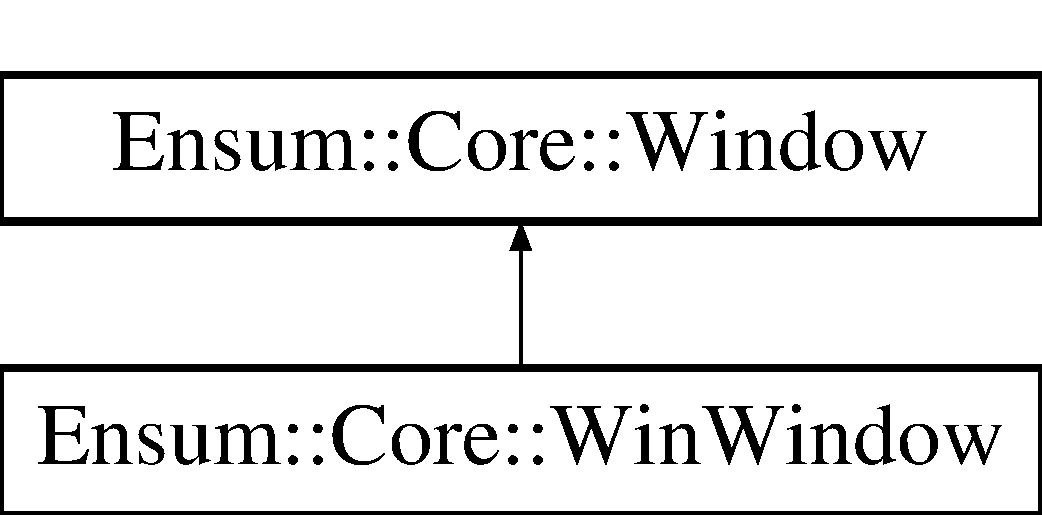
\includegraphics[height=2.000000cm]{class_ensum_1_1_core_1_1_window}
\end{center}
\end{figure}
\subsection*{Public Member Functions}
\begin{DoxyCompactItemize}
\item 
virtual const void \hyperlink{class_ensum_1_1_core_1_1_window_a43f467e7e5ea83f3a9b990b6edc2ec46}{Init} ()=0\hypertarget{class_ensum_1_1_core_1_1_window_a43f467e7e5ea83f3a9b990b6edc2ec46}{}\label{class_ensum_1_1_core_1_1_window_a43f467e7e5ea83f3a9b990b6edc2ec46}

\begin{DoxyCompactList}\small\item\em Initialization for the window. \end{DoxyCompactList}\item 
virtual const void \hyperlink{class_ensum_1_1_core_1_1_window_aeafece8bb46d29de1de3ddf092662195}{Start} ()=0\hypertarget{class_ensum_1_1_core_1_1_window_aeafece8bb46d29de1de3ddf092662195}{}\label{class_ensum_1_1_core_1_1_window_aeafece8bb46d29de1de3ddf092662195}

\begin{DoxyCompactList}\small\item\em Start the message loop. \end{DoxyCompactList}\item 
\hyperlink{class_ensum_1_1_input_1_1_input}{Input\+::\+Input} $\ast$ \hyperlink{class_ensum_1_1_core_1_1_window_af746ffdd0281b2722d162fbf96c3542b}{Get\+Input} ()\hypertarget{class_ensum_1_1_core_1_1_window_af746ffdd0281b2722d162fbf96c3542b}{}\label{class_ensum_1_1_core_1_1_window_af746ffdd0281b2722d162fbf96c3542b}

\begin{DoxyCompactList}\small\item\em Returns a pointer to the input. \end{DoxyCompactList}\end{DoxyCompactItemize}
\subsection*{Static Public Member Functions}
\begin{DoxyCompactItemize}
\item 
static \hyperlink{class_ensum_1_1_core_1_1_window}{Window} $\ast$ \hyperlink{class_ensum_1_1_core_1_1_window_af9478f4a6643763ba3be7a1a9fc98377}{Create\+Win} (\hyperlink{class_ensum_1_1_core_1_1_window}{Window} $\ast$window)\hypertarget{class_ensum_1_1_core_1_1_window_af9478f4a6643763ba3be7a1a9fc98377}{}\label{class_ensum_1_1_core_1_1_window_af9478f4a6643763ba3be7a1a9fc98377}

\begin{DoxyCompactList}\small\item\em Saves the given window and initializes it. \end{DoxyCompactList}\item 
static \hyperlink{class_ensum_1_1_core_1_1_window}{Window} $\ast$ \hyperlink{class_ensum_1_1_core_1_1_window_ada827fab647cc63b1c389f91f670bf18}{Get\+Instance} ()\hypertarget{class_ensum_1_1_core_1_1_window_ada827fab647cc63b1c389f91f670bf18}{}\label{class_ensum_1_1_core_1_1_window_ada827fab647cc63b1c389f91f670bf18}

\begin{DoxyCompactList}\small\item\em Returns a pointer to the window. \end{DoxyCompactList}\item 
static void \hyperlink{class_ensum_1_1_core_1_1_window_ac6e8b05158fca2587cdfe23dabf35baf}{Delete\+Instance} ()
\begin{DoxyCompactList}\small\item\em Deletes the window. \end{DoxyCompactList}\end{DoxyCompactItemize}
\subsection*{Public Attributes}
\begin{DoxyCompactItemize}
\item 
\hyperlink{class_ensum_1_1_utils_1_1_event}{Utils\+::\+Event}$<$ const void()$>$ {\bfseries Frame\+Start}\hypertarget{class_ensum_1_1_core_1_1_window_ad122b1a7fa3fdfcb351abbad2252dfe2}{}\label{class_ensum_1_1_core_1_1_window_ad122b1a7fa3fdfcb351abbad2252dfe2}

\end{DoxyCompactItemize}
\subsection*{Protected Member Functions}
\begin{DoxyCompactItemize}
\item 
virtual const void \hyperlink{class_ensum_1_1_core_1_1_window_a58af9c1b06e0fe12820f584f4638ae15}{Frame} ()=0
\begin{DoxyCompactList}\small\item\em The frame function. \end{DoxyCompactList}\end{DoxyCompactItemize}
\subsection*{Protected Attributes}
\begin{DoxyCompactItemize}
\item 
\hyperlink{class_ensum_1_1_core_1_1_timer}{Timer} $\ast$ {\bfseries \+\_\+timer}\hypertarget{class_ensum_1_1_core_1_1_window_aa27d25534350ec8e46cf2eae67c82ea5}{}\label{class_ensum_1_1_core_1_1_window_aa27d25534350ec8e46cf2eae67c82ea5}

\item 
\hyperlink{class_ensum_1_1_input_1_1_input}{Input\+::\+Input} $\ast$ {\bfseries \+\_\+input}\hypertarget{class_ensum_1_1_core_1_1_window_a6b2925a490f7a5a2417059660713bc19}{}\label{class_ensum_1_1_core_1_1_window_a6b2925a490f7a5a2417059660713bc19}

\end{DoxyCompactItemize}
\subsection*{Static Protected Attributes}
\begin{DoxyCompactItemize}
\item 
static \hyperlink{class_ensum_1_1_core_1_1_window}{Window} $\ast$ {\bfseries \+\_\+instance}\hypertarget{class_ensum_1_1_core_1_1_window_aa4ca94e77186512ab2949dd6c7e850e6}{}\label{class_ensum_1_1_core_1_1_window_aa4ca94e77186512ab2949dd6c7e850e6}

\end{DoxyCompactItemize}


\subsection{Detailed Description}
Fully abstract class for interfacting with the actual window. 

\subsection{Member Function Documentation}
\index{Ensum\+::\+Core\+::\+Window@{Ensum\+::\+Core\+::\+Window}!Delete\+Instance@{Delete\+Instance}}
\index{Delete\+Instance@{Delete\+Instance}!Ensum\+::\+Core\+::\+Window@{Ensum\+::\+Core\+::\+Window}}
\subsubsection[{\texorpdfstring{Delete\+Instance()}{DeleteInstance()}}]{\setlength{\rightskip}{0pt plus 5cm}static void Ensum\+::\+Core\+::\+Window\+::\+Delete\+Instance (
\begin{DoxyParamCaption}
{}
\end{DoxyParamCaption}
)\hspace{0.3cm}{\ttfamily [static]}}\hypertarget{class_ensum_1_1_core_1_1_window_ac6e8b05158fca2587cdfe23dabf35baf}{}\label{class_ensum_1_1_core_1_1_window_ac6e8b05158fca2587cdfe23dabf35baf}


Deletes the window. 

This also deletes all members \index{Ensum\+::\+Core\+::\+Window@{Ensum\+::\+Core\+::\+Window}!Frame@{Frame}}
\index{Frame@{Frame}!Ensum\+::\+Core\+::\+Window@{Ensum\+::\+Core\+::\+Window}}
\subsubsection[{\texorpdfstring{Frame()=0}{Frame()=0}}]{\setlength{\rightskip}{0pt plus 5cm}virtual const void Ensum\+::\+Core\+::\+Window\+::\+Frame (
\begin{DoxyParamCaption}
{}
\end{DoxyParamCaption}
)\hspace{0.3cm}{\ttfamily [protected]}, {\ttfamily [pure virtual]}}\hypertarget{class_ensum_1_1_core_1_1_window_a58af9c1b06e0fe12820f584f4638ae15}{}\label{class_ensum_1_1_core_1_1_window_a58af9c1b06e0fe12820f584f4638ae15}


The frame function. 

Put the gamelogic here. 

Implemented in \hyperlink{class_ensum_1_1_core_1_1_win_window_a3e828ccbc90f0d6ed81c2320277561e6}{Ensum\+::\+Core\+::\+Win\+Window}.



The documentation for this class was generated from the following file\+:\begin{DoxyCompactItemize}
\item 
Includes/\+Ensum\+\_\+core/Window.\+h\end{DoxyCompactItemize}

\hypertarget{class_ensum_1_1_core_1_1_win_window}{}\section{Ensum\+:\+:Core\+:\+:Win\+Window Class Reference}
\label{class_ensum_1_1_core_1_1_win_window}\index{Ensum\+::\+Core\+::\+Win\+Window@{Ensum\+::\+Core\+::\+Win\+Window}}


Windows specific window.  




{\ttfamily \#include $<$Windows\+Window.\+h$>$}

Inheritance diagram for Ensum\+:\+:Core\+:\+:Win\+Window\+:\begin{figure}[H]
\begin{center}
\leavevmode
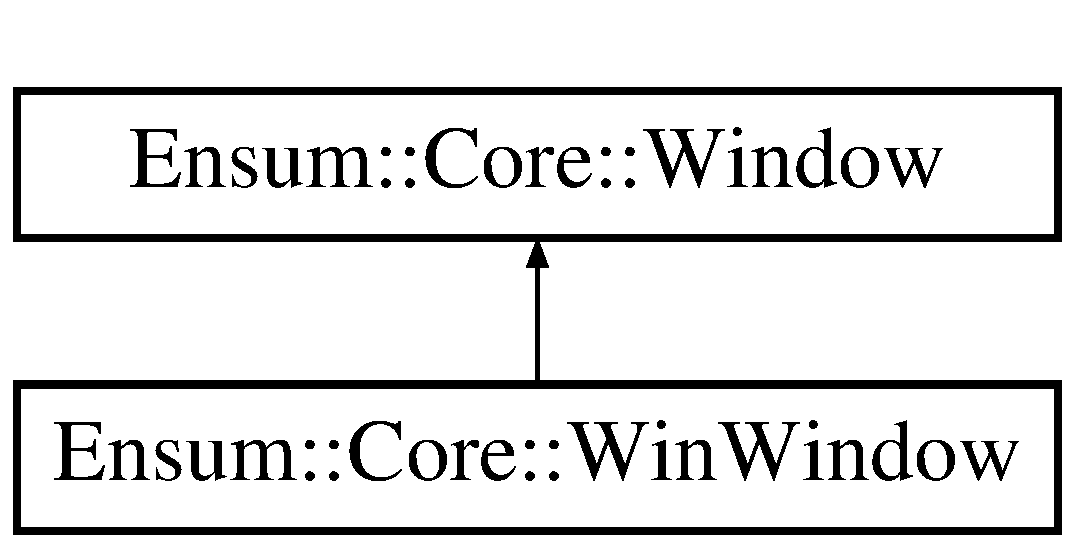
\includegraphics[height=2.000000cm]{class_ensum_1_1_core_1_1_win_window}
\end{center}
\end{figure}
\subsection*{Public Member Functions}
\begin{DoxyCompactItemize}
\item 
virtual const void \hyperlink{class_ensum_1_1_core_1_1_win_window_afb59ce364f98918b2b17653cbfc39ead}{Init} ()\hypertarget{class_ensum_1_1_core_1_1_win_window_afb59ce364f98918b2b17653cbfc39ead}{}\label{class_ensum_1_1_core_1_1_win_window_afb59ce364f98918b2b17653cbfc39ead}

\begin{DoxyCompactList}\small\item\em Initialization for the window. \end{DoxyCompactList}\item 
virtual const void \hyperlink{class_ensum_1_1_core_1_1_win_window_a1c316902d186c3d685210237e3438745}{Start} ()\hypertarget{class_ensum_1_1_core_1_1_win_window_a1c316902d186c3d685210237e3438745}{}\label{class_ensum_1_1_core_1_1_win_window_a1c316902d186c3d685210237e3438745}

\begin{DoxyCompactList}\small\item\em Start the message loop. \end{DoxyCompactList}\end{DoxyCompactItemize}
\subsection*{Protected Member Functions}
\begin{DoxyCompactItemize}
\item 
virtual const void \hyperlink{class_ensum_1_1_core_1_1_win_window_a3e828ccbc90f0d6ed81c2320277561e6}{Frame} ()
\begin{DoxyCompactList}\small\item\em The frame function. \end{DoxyCompactList}\end{DoxyCompactItemize}
\subsection*{Protected Attributes}
\begin{DoxyCompactItemize}
\item 
H\+I\+N\+S\+T\+A\+N\+CE {\bfseries \+\_\+h\+Inst}\hypertarget{class_ensum_1_1_core_1_1_win_window_a19562456a0e7d38dc67b673ad8c0a9ea}{}\label{class_ensum_1_1_core_1_1_win_window_a19562456a0e7d38dc67b673ad8c0a9ea}

\item 
H\+W\+ND {\bfseries \+\_\+h\+Wnd}\hypertarget{class_ensum_1_1_core_1_1_win_window_af0bdb075823585bf3f99895ab4dcfffa}{}\label{class_ensum_1_1_core_1_1_win_window_af0bdb075823585bf3f99895ab4dcfffa}

\item 
D\+W\+O\+RD {\bfseries \+\_\+style}\hypertarget{class_ensum_1_1_core_1_1_win_window_af2bbdea21686b0d5a38bd3c85bc8f7db}{}\label{class_ensum_1_1_core_1_1_win_window_af2bbdea21686b0d5a38bd3c85bc8f7db}

\item 
L\+P\+W\+S\+TR {\bfseries \+\_\+wnd\+Caption}\hypertarget{class_ensum_1_1_core_1_1_win_window_a75879298465e6dab7671f0028489f82a}{}\label{class_ensum_1_1_core_1_1_win_window_a75879298465e6dab7671f0028489f82a}

\item 
bool {\bfseries \+\_\+running}\hypertarget{class_ensum_1_1_core_1_1_win_window_a11e86f63066c9cb730c152b23f2e5378}{}\label{class_ensum_1_1_core_1_1_win_window_a11e86f63066c9cb730c152b23f2e5378}

\end{DoxyCompactItemize}
\subsection*{Additional Inherited Members}


\subsection{Detailed Description}
Windows specific window. 

\subsection{Member Function Documentation}
\index{Ensum\+::\+Core\+::\+Win\+Window@{Ensum\+::\+Core\+::\+Win\+Window}!Frame@{Frame}}
\index{Frame@{Frame}!Ensum\+::\+Core\+::\+Win\+Window@{Ensum\+::\+Core\+::\+Win\+Window}}
\subsubsection[{\texorpdfstring{Frame()}{Frame()}}]{\setlength{\rightskip}{0pt plus 5cm}virtual const void Ensum\+::\+Core\+::\+Win\+Window\+::\+Frame (
\begin{DoxyParamCaption}
{}
\end{DoxyParamCaption}
)\hspace{0.3cm}{\ttfamily [protected]}, {\ttfamily [virtual]}}\hypertarget{class_ensum_1_1_core_1_1_win_window_a3e828ccbc90f0d6ed81c2320277561e6}{}\label{class_ensum_1_1_core_1_1_win_window_a3e828ccbc90f0d6ed81c2320277561e6}


The frame function. 

Put the gamelogic here. 

Implements \hyperlink{class_ensum_1_1_core_1_1_window_a58af9c1b06e0fe12820f584f4638ae15}{Ensum\+::\+Core\+::\+Window}.



The documentation for this class was generated from the following file\+:\begin{DoxyCompactItemize}
\item 
Includes/\+Ensum\+\_\+core/Windows\+Window.\+h\end{DoxyCompactItemize}

%--- End generated contents ---

% Index
\backmatter
\newpage
\phantomsection
\clearemptydoublepage
\addcontentsline{toc}{chapter}{Index}
\printindex

\end{document}
